\chapter{Design}

\section{Architecture}

The architecture of the system is similar to that of the open-source
\emph{Bacula} project, in that it is organised into separate modules. Figure
\ref{fig:architecture} shows the high-level layout of the design, with arrows
to represent the flow of data.

\begin{figure}[h]
    \setlength{\unitlength}{0.14in}
    \centering
    \footnotesize
    \begin{picture}(28,21)
        \put(10,8){\framebox(8,4){backtracserverd}}
        \put(14,8){\vector(0,-1){4}}
        \put(14,4){\vector(0,1){4}}
        \put(10,0){\framebox(8,4){backtracweb}}
        \put(14,16){\vector(0,-1){4}}
        \put(14,12){\vector(0,1){4}}
        \put(10,16){\framebox(8,4){backtracd}}
        \put(18,10){\vector(3,-2){6}}
        \put(24,6){\vector(-3,2){6}}
        \put(24,4){\umlDatabaseLbl{DB}}
        \put(18,2){\vector(3,2){6}}
        \put(24,6){\vector(-3,-2){6}}
        \put(0,4.5){\framebox(6,3){Storage}}
        \put(6,6){\vector(1,1){4}}
        \put(10,10){\vector(-1,-1){4}}
        \put(6,6){\vector(1,-1){4}}
        \put(0,12){\umlRaid}
        \put(3,7.5){\vector(0,1){4.5}}
        \put(3,12){\vector(0,-1){4.5}}
    \end{picture}
    \caption{Diagram showing the implemented system architecture}
    \label{fig:architecture}
\end{figure}

At the centre of the system is the server daemon, \emph{backtracserverd}.  It
is this program that maintains a connection to the client daemon,
\emph{backtracd}, which is installed and running on each protected client.

The server daemon also has access to a database, which is used to store not
only the meta-data relating to files protected by the system, but also to the
hosts that it protects. This database is called the \emph{catalog}.

The \emph{storage} subsystem provides an interface for the server daemon to
read and write files to the physical disk, whilst not explicitly choosing their
location or name. This level of abstraction provides extensibility, should
a future implementation change be desired (for example, cloud storage).

The web interface (denoted as \emph{backtracweb} in Figure
\ref{fig:architecture}) allows the administrator to manage and monitor all
aspects of the backup system. The application has read and write access to the
database so clients can be added or altered, and existing clients can be
inspected. Also, read-only access to the storage subsystem is permitted,
allowing the administrator to download files from the archive through the web
interface.

The server daemon and the web interface, though separate programs in their own
right, are intended to run on the same host---the \emph{backup server}.

The database, provided by an RDBMS such as MySQL or PostgreSQL (or SQLite for
smaller installations), can reside on host that is separate to the backup
server. For example, if an existing database server is already installed and
running at a particular site, that server may be used for storing the catalog.

\section{Catalog}

\begin{figure}
    \begin{center}
        \newlength{\svgwidth}
        \setlength{\svgwidth}{1.1\textwidth}
        \tiny
        %LaTeX with PSTricks extensions
%%Creator: inkscape 0.48.0
%%Please note this file requires PSTricks extensions
\psset{xunit=.5pt,yunit=.5pt,runit=.5pt}
\begin{pspicture}(791.5,460)
{
\newrgbcolor{curcolor}{0 0 0}
\pscustom[linewidth=1,linecolor=curcolor]
{
\newpath
\moveto(245.5,446.5)
\lineto(365.02191162,446.5)
\lineto(365.02191162,427.5)
\lineto(245.5,427.5)
\closepath
}
}
{
\newrgbcolor{curcolor}{0 0 0}
\pscustom[linewidth=1,linecolor=curcolor]
{
\newpath
\moveto(245.5,427.5)
\lineto(365.02191162,427.5)
\lineto(365.02191162,386.5)
\lineto(245.5,386.5)
\closepath
}
}
{
\newrgbcolor{curcolor}{0 0 0}
\pscustom[linestyle=none,fillstyle=solid,fillcolor=curcolor]
{
\newpath
\moveto(287.5703125,436.79492188)
\lineto(289.2578125,436.95898438)
\curveto(289.35937278,436.39257573)(289.5644507,435.97656052)(289.87304688,435.7109375)
\curveto(290.18554383,435.44531105)(290.60546528,435.31249869)(291.1328125,435.3125)
\curveto(291.6914017,435.31249869)(292.11132315,435.42968607)(292.39257812,435.6640625)
\curveto(292.67772883,435.90234185)(292.82030682,436.17968532)(292.8203125,436.49609375)
\curveto(292.82030682,436.69921605)(292.75976,436.87109088)(292.63867188,437.01171875)
\curveto(292.52147899,437.15624684)(292.31444795,437.28124672)(292.01757812,437.38671875)
\curveto(291.81444845,437.45702779)(291.35155829,437.58202767)(290.62890625,437.76171875)
\curveto(289.69921619,437.99218351)(289.04687309,438.27538635)(288.671875,438.61132812)
\curveto(288.14453024,439.08397929)(287.88085863,439.66015059)(287.88085938,440.33984375)
\curveto(287.88085863,440.77733697)(288.00390538,441.18553969)(288.25,441.56445312)
\curveto(288.49999864,441.94725768)(288.85742015,442.23827301)(289.32226562,442.4375)
\curveto(289.79101297,442.63671011)(290.35546553,442.73631939)(291.015625,442.73632812)
\curveto(292.09374504,442.73631939)(292.90429111,442.4999915)(293.44726562,442.02734375)
\curveto(293.99413377,441.55467995)(294.28124286,440.9238212)(294.30859375,440.13476562)
\lineto(292.57421875,440.05859375)
\curveto(292.49999464,440.4999935)(292.33983855,440.81639943)(292.09375,441.0078125)
\curveto(291.85155779,441.2031178)(291.48632378,441.30077395)(290.99804688,441.30078125)
\curveto(290.49413727,441.30077395)(290.09960641,441.19725843)(289.81445312,440.99023438)
\curveto(289.63085688,440.85741502)(289.5390601,440.67968082)(289.5390625,440.45703125)
\curveto(289.5390601,440.2539)(289.62499751,440.08007204)(289.796875,439.93554688)
\curveto(290.01562212,439.75194737)(290.54687159,439.56054131)(291.390625,439.36132812)
\curveto(292.2343699,439.16210421)(292.85741615,438.95507317)(293.25976562,438.74023438)
\curveto(293.6660091,438.52929235)(293.98241503,438.23827701)(294.20898438,437.8671875)
\curveto(294.43944582,437.4999965)(294.55468008,437.04491883)(294.5546875,436.50195312)
\curveto(294.55468008,436.00976362)(294.41796147,435.54882658)(294.14453125,435.11914062)
\curveto(293.87108702,434.68945244)(293.48436865,434.36914026)(292.984375,434.15820312)
\curveto(292.48436965,433.95117192)(291.8613234,433.8476564)(291.11523438,433.84765625)
\curveto(290.02929398,433.8476564)(289.19531044,434.09765615)(288.61328125,434.59765625)
\curveto(288.03124911,435.1015614)(287.6835932,435.83398254)(287.5703125,436.79492188)
}
}
{
\newrgbcolor{curcolor}{0 0 0}
\pscustom[linestyle=none,fillstyle=solid,fillcolor=curcolor]
{
\newpath
\moveto(298.8671875,440.22265625)
\lineto(298.8671875,438.91015625)
\lineto(297.7421875,438.91015625)
\lineto(297.7421875,436.40234375)
\curveto(297.74218491,435.89452936)(297.75195053,435.59765465)(297.77148438,435.51171875)
\curveto(297.79491923,435.42968607)(297.84374731,435.36132676)(297.91796875,435.30664062)
\curveto(297.99609091,435.25195187)(298.08984081,435.22460815)(298.19921875,435.22460938)
\curveto(298.3515593,435.22460815)(298.57226221,435.27734247)(298.86132812,435.3828125)
\lineto(299.00195312,434.10546875)
\curveto(298.61913716,433.94140631)(298.18554384,433.85937514)(297.70117188,433.859375)
\curveto(297.40429462,433.85937514)(297.13671677,433.90820322)(296.8984375,434.00585938)
\curveto(296.66015474,434.10742177)(296.48437367,434.23632789)(296.37109375,434.39257812)
\curveto(296.26171764,434.55273382)(296.18554584,434.76757736)(296.14257812,435.03710938)
\curveto(296.10742092,435.2285144)(296.08984281,435.61523276)(296.08984375,436.19726562)
\lineto(296.08984375,438.91015625)
\lineto(295.33398438,438.91015625)
\lineto(295.33398438,440.22265625)
\lineto(296.08984375,440.22265625)
\lineto(296.08984375,441.45898438)
\lineto(297.7421875,442.41992188)
\lineto(297.7421875,440.22265625)
\lineto(298.8671875,440.22265625)
}
}
{
\newrgbcolor{curcolor}{0 0 0}
\pscustom[linestyle=none,fillstyle=solid,fillcolor=curcolor]
{
\newpath
\moveto(301.25195312,438.32421875)
\lineto(299.7578125,438.59375)
\curveto(299.92578048,439.1953073)(300.2148427,439.64061936)(300.625,439.9296875)
\curveto(301.03515437,440.21874378)(301.64452877,440.36327489)(302.453125,440.36328125)
\curveto(303.18749597,440.36327489)(303.73437043,440.27538435)(304.09375,440.09960938)
\curveto(304.45311971,439.92772845)(304.70507258,439.70702554)(304.84960938,439.4375)
\curveto(304.99804104,439.17186983)(305.07225971,438.68163594)(305.07226562,437.96679688)
\lineto(305.0546875,436.04492188)
\curveto(305.05468161,435.49804538)(305.08007221,435.09374891)(305.13085938,434.83203125)
\curveto(305.18554085,434.57421818)(305.28515012,434.2968747)(305.4296875,434)
\lineto(303.80078125,434)
\curveto(303.7578079,434.10937489)(303.70507358,434.2714841)(303.64257812,434.48632812)
\curveto(303.61522992,434.58398379)(303.59569869,434.64843685)(303.58398438,434.6796875)
\curveto(303.30273023,434.40624959)(303.00194928,434.20117167)(302.68164062,434.06445312)
\curveto(302.36132492,433.92773445)(302.01952839,433.85937514)(301.65625,433.859375)
\curveto(301.01562314,433.85937514)(300.50976428,434.03320309)(300.13867188,434.38085938)
\curveto(299.77148376,434.7285149)(299.5878902,435.16796758)(299.58789062,435.69921875)
\curveto(299.5878902,436.0507792)(299.67187449,436.36327889)(299.83984375,436.63671875)
\curveto(300.00781165,436.91405959)(300.24218642,437.12499688)(300.54296875,437.26953125)
\curveto(300.84765456,437.41796533)(301.28515413,437.54687145)(301.85546875,437.65625)
\curveto(302.62499654,437.80077745)(303.15819913,437.93554294)(303.45507812,438.06054688)
\lineto(303.45507812,438.22460938)
\curveto(303.45507383,438.54101108)(303.37694891,438.76562023)(303.22070312,438.8984375)
\curveto(303.06444922,439.03515121)(302.76952764,439.10351052)(302.3359375,439.10351562)
\curveto(302.04296587,439.10351052)(301.81445047,439.04491683)(301.65039062,438.92773438)
\curveto(301.4863258,438.81444831)(301.35351343,438.61327664)(301.25195312,438.32421875)
\moveto(303.45507812,436.98828125)
\curveto(303.24413654,436.91796583)(302.9101525,436.83398154)(302.453125,436.73632812)
\curveto(301.99609091,436.63866924)(301.69726309,436.54296621)(301.55664062,436.44921875)
\curveto(301.34179469,436.2968727)(301.23437293,436.10351352)(301.234375,435.86914062)
\curveto(301.23437293,435.63867024)(301.32031034,435.43945169)(301.4921875,435.27148438)
\curveto(301.66406,435.10351452)(301.88280978,435.01953023)(302.1484375,435.01953125)
\curveto(302.44530921,435.01953023)(302.72851206,435.11718638)(302.99804688,435.3125)
\curveto(303.19726159,435.46093604)(303.32812083,435.64257648)(303.390625,435.85742188)
\curveto(303.43358948,435.99804488)(303.45507383,436.26562273)(303.45507812,436.66015625)
\lineto(303.45507812,436.98828125)
}
}
{
\newrgbcolor{curcolor}{0 0 0}
\pscustom[linestyle=none,fillstyle=solid,fillcolor=curcolor]
{
\newpath
\moveto(309.5546875,440.22265625)
\lineto(309.5546875,438.91015625)
\lineto(308.4296875,438.91015625)
\lineto(308.4296875,436.40234375)
\curveto(308.42968491,435.89452936)(308.43945053,435.59765465)(308.45898438,435.51171875)
\curveto(308.48241923,435.42968607)(308.53124731,435.36132676)(308.60546875,435.30664062)
\curveto(308.68359091,435.25195187)(308.77734081,435.22460815)(308.88671875,435.22460938)
\curveto(309.0390593,435.22460815)(309.25976221,435.27734247)(309.54882812,435.3828125)
\lineto(309.68945312,434.10546875)
\curveto(309.30663716,433.94140631)(308.87304384,433.85937514)(308.38867188,433.859375)
\curveto(308.09179462,433.85937514)(307.82421677,433.90820322)(307.5859375,434.00585938)
\curveto(307.34765474,434.10742177)(307.17187367,434.23632789)(307.05859375,434.39257812)
\curveto(306.94921764,434.55273382)(306.87304584,434.76757736)(306.83007812,435.03710938)
\curveto(306.79492092,435.2285144)(306.77734281,435.61523276)(306.77734375,436.19726562)
\lineto(306.77734375,438.91015625)
\lineto(306.02148438,438.91015625)
\lineto(306.02148438,440.22265625)
\lineto(306.77734375,440.22265625)
\lineto(306.77734375,441.45898438)
\lineto(308.4296875,442.41992188)
\lineto(308.4296875,440.22265625)
\lineto(309.5546875,440.22265625)
}
}
{
\newrgbcolor{curcolor}{0 0 0}
\pscustom[linestyle=none,fillstyle=solid,fillcolor=curcolor]
{
\newpath
\moveto(314.8046875,434)
\lineto(314.8046875,434.93164062)
\curveto(314.57812027,434.59960878)(314.27929244,434.33789029)(313.90820312,434.14648438)
\curveto(313.54101193,433.95507817)(313.15234045,433.85937514)(312.7421875,433.859375)
\curveto(312.32421627,433.85937514)(311.94921665,433.95117192)(311.6171875,434.13476562)
\curveto(311.28515481,434.31835906)(311.04492068,434.5761713)(310.89648438,434.90820312)
\curveto(310.74804597,435.24023313)(310.6738273,435.69921705)(310.67382812,436.28515625)
\lineto(310.67382812,440.22265625)
\lineto(312.3203125,440.22265625)
\lineto(312.3203125,437.36328125)
\curveto(312.32031003,436.48827876)(312.34960687,435.95116992)(312.40820312,435.75195312)
\curveto(312.4707005,435.55663907)(312.58202852,435.40038922)(312.7421875,435.28320312)
\curveto(312.9023407,435.16992071)(313.10546549,435.11328014)(313.3515625,435.11328125)
\curveto(313.63280871,435.11328014)(313.88476159,435.18945194)(314.10742188,435.34179688)
\curveto(314.33007364,435.49804538)(314.48241724,435.68945144)(314.56445312,435.91601562)
\curveto(314.64647958,436.14648223)(314.68749516,436.70702854)(314.6875,437.59765625)
\lineto(314.6875,440.22265625)
\lineto(316.33398438,440.22265625)
\lineto(316.33398438,434)
\lineto(314.8046875,434)
}
}
{
\newrgbcolor{curcolor}{0 0 0}
\pscustom[linestyle=none,fillstyle=solid,fillcolor=curcolor]
{
\newpath
\moveto(317.46484375,435.77539062)
\lineto(319.1171875,436.02734375)
\curveto(319.187498,435.70702954)(319.33007598,435.46288916)(319.54492188,435.29492188)
\curveto(319.75976305,435.13085824)(320.060544,435.04882708)(320.44726562,435.04882812)
\curveto(320.87304319,435.04882708)(321.19335537,435.126952)(321.40820312,435.28320312)
\curveto(321.55273001,435.39257673)(321.62499556,435.53906096)(321.625,435.72265625)
\curveto(321.62499556,435.8476544)(321.5859331,435.95116992)(321.5078125,436.03320312)
\curveto(321.42577701,436.11132601)(321.24218344,436.18359157)(320.95703125,436.25)
\curveto(319.6289038,436.54296621)(318.78710777,436.81054406)(318.43164062,437.05273438)
\curveto(317.93945237,437.38866849)(317.69335887,437.85546489)(317.69335938,438.453125)
\curveto(317.69335887,438.99218251)(317.90624928,439.44530705)(318.33203125,439.8125)
\curveto(318.75781093,440.17968132)(319.41796652,440.36327489)(320.3125,440.36328125)
\curveto(321.16405852,440.36327489)(321.79687039,440.22460315)(322.2109375,439.94726562)
\curveto(322.62499456,439.66991621)(322.91015052,439.25976037)(323.06640625,438.71679688)
\lineto(321.51367188,438.4296875)
\curveto(321.44726136,438.67187033)(321.32030836,438.85741702)(321.1328125,438.98632812)
\curveto(320.94921498,439.11522926)(320.68554337,439.17968232)(320.34179688,439.1796875)
\curveto(319.9082004,439.17968232)(319.59765384,439.11913551)(319.41015625,438.99804688)
\curveto(319.28515415,438.91210446)(319.22265421,438.80077645)(319.22265625,438.6640625)
\curveto(319.22265421,438.54687045)(319.27734166,438.44726118)(319.38671875,438.36523438)
\curveto(319.5351539,438.25585512)(320.04687214,438.1015584)(320.921875,437.90234375)
\curveto(321.80077663,437.7031213)(322.41405727,437.45898092)(322.76171875,437.16992188)
\curveto(323.10546283,436.87695025)(323.27733766,436.46874753)(323.27734375,435.9453125)
\curveto(323.27733766,435.37499862)(323.03905664,434.88476474)(322.5625,434.47460938)
\curveto(322.0859326,434.06445306)(321.38085518,433.85937514)(320.44726562,433.859375)
\curveto(319.59960696,433.85937514)(318.92773263,434.03124997)(318.43164062,434.375)
\curveto(317.93945237,434.71874928)(317.61718707,435.18554569)(317.46484375,435.77539062)
}
}
{
\newrgbcolor{curcolor}{0.40000001 0.40000001 0.40000001}
\pscustom[linestyle=none,fillstyle=solid,fillcolor=curcolor]
{
\newpath
\moveto(269.57617188,412.5)
\lineto(269.57617188,421.08984375)
\lineto(270.71289062,421.08984375)
\lineto(270.71289062,412.5)
\lineto(269.57617188,412.5)
}
}
{
\newrgbcolor{curcolor}{0.40000001 0.40000001 0.40000001}
\pscustom[linestyle=none,fillstyle=solid,fillcolor=curcolor]
{
\newpath
\moveto(272.15429688,414.35742188)
\lineto(273.19726562,414.52148438)
\curveto(273.2558579,414.10351402)(273.41796712,413.78320184)(273.68359375,413.56054688)
\curveto(273.95312283,413.33788979)(274.32812246,413.22656177)(274.80859375,413.2265625)
\curveto(275.29296524,413.22656177)(275.65233988,413.32421793)(275.88671875,413.51953125)
\curveto(276.12108941,413.71874878)(276.2382768,413.95117042)(276.23828125,414.21679688)
\curveto(276.2382768,414.45507617)(276.13476128,414.64257598)(275.92773438,414.77929688)
\curveto(275.78319913,414.8730445)(275.42382449,414.99218501)(274.84960938,415.13671875)
\curveto(274.07616958,415.33202842)(273.53906075,415.499997)(273.23828125,415.640625)
\curveto(272.94140509,415.78515296)(272.71484282,415.98241839)(272.55859375,416.23242188)
\curveto(272.40624938,416.48632414)(272.33007758,416.76562073)(272.33007812,417.0703125)
\curveto(272.33007758,417.3476514)(272.39257752,417.60351052)(272.51757812,417.83789062)
\curveto(272.64648351,418.0761663)(272.82031146,418.27343173)(273.0390625,418.4296875)
\curveto(273.20312358,418.5507752)(273.42577961,418.6523376)(273.70703125,418.734375)
\curveto(273.99218529,418.82030618)(274.29687249,418.86327489)(274.62109375,418.86328125)
\curveto(275.10937168,418.86327489)(275.53710562,418.79296246)(275.90429688,418.65234375)
\curveto(276.27538613,418.51171274)(276.54882336,418.32030668)(276.72460938,418.078125)
\curveto(276.90038551,417.83983841)(277.02147914,417.51952623)(277.08789062,417.1171875)
\lineto(276.05664062,416.9765625)
\curveto(276.0097614,417.2968702)(275.87304279,417.54686995)(275.64648438,417.7265625)
\curveto(275.42382449,417.90624459)(275.10741855,417.99608825)(274.69726562,417.99609375)
\curveto(274.2128882,417.99608825)(273.86718542,417.91601021)(273.66015625,417.75585938)
\curveto(273.45312333,417.59569803)(273.34960781,417.40819822)(273.34960938,417.19335938)
\curveto(273.34960781,417.05663607)(273.39257652,416.93358932)(273.47851562,416.82421875)
\curveto(273.56445135,416.71093329)(273.69921684,416.61718338)(273.8828125,416.54296875)
\curveto(273.98827905,416.50390225)(274.29882561,416.41405859)(274.81445312,416.2734375)
\curveto(275.5605431,416.07421518)(276.08007383,415.91015284)(276.37304688,415.78125)
\curveto(276.66991699,415.65624684)(276.90233863,415.47265328)(277.0703125,415.23046875)
\curveto(277.2382758,414.98827876)(277.32226009,414.68749781)(277.32226562,414.328125)
\curveto(277.32226009,413.97656102)(277.21874457,413.64453011)(277.01171875,413.33203125)
\curveto(276.80858873,413.02343698)(276.51366715,412.78320284)(276.12695312,412.61132812)
\curveto(275.74023042,412.44335943)(275.30273086,412.35937514)(274.81445312,412.359375)
\curveto(274.00585715,412.35937514)(273.38867027,412.52734372)(272.96289062,412.86328125)
\curveto(272.54101487,413.19921805)(272.27148389,413.69726443)(272.15429688,414.35742188)
}
}
{
\newrgbcolor{curcolor}{0.40000001 0.40000001 0.40000001}
\pscustom[linestyle=none,fillstyle=solid,fillcolor=curcolor]
{
\newpath
\moveto(277.60351562,410.11523438)
\lineto(277.60351562,410.87695312)
\lineto(284.59375,410.87695312)
\lineto(284.59375,410.11523438)
\lineto(277.60351562,410.11523438)
}
}
{
\newrgbcolor{curcolor}{0.40000001 0.40000001 0.40000001}
\pscustom[linestyle=none,fillstyle=solid,fillcolor=curcolor]
{
\newpath
\moveto(291.51953125,415.51171875)
\lineto(292.65625,415.22460938)
\curveto(292.4179608,414.29101383)(291.98827373,413.57812392)(291.3671875,413.0859375)
\curveto(290.74999371,412.59765615)(289.9941351,412.35351577)(289.09960938,412.35351562)
\curveto(288.17382442,412.35351577)(287.41991892,412.54101558)(286.83789062,412.91601562)
\curveto(286.25976383,413.29492108)(285.81835802,413.84179553)(285.51367188,414.55664062)
\curveto(285.21288988,415.2714816)(285.0624994,416.03905896)(285.0625,416.859375)
\curveto(285.0624994,417.753901)(285.23242111,418.53319709)(285.57226562,419.19726562)
\curveto(285.91601417,419.86522701)(286.40234181,420.37108588)(287.03125,420.71484375)
\curveto(287.6640593,421.06249144)(288.35937111,421.23631939)(289.1171875,421.23632812)
\curveto(289.97655699,421.23631939)(290.69921252,421.01756961)(291.28515625,420.58007812)
\curveto(291.87108634,420.14257048)(292.27928906,419.52733672)(292.50976562,418.734375)
\lineto(291.390625,418.47070312)
\curveto(291.19139952,419.09569653)(290.90233731,419.5507742)(290.5234375,419.8359375)
\curveto(290.14452557,420.12108613)(289.66796355,420.26366411)(289.09375,420.26367188)
\curveto(288.43358978,420.26366411)(287.88085596,420.10546114)(287.43554688,419.7890625)
\curveto(286.9941381,419.47264928)(286.68359153,419.04686845)(286.50390625,418.51171875)
\curveto(286.32421689,417.98046327)(286.23437323,417.43163569)(286.234375,416.86523438)
\curveto(286.23437323,416.13476199)(286.33984187,415.49609075)(286.55078125,414.94921875)
\curveto(286.7656227,414.40624809)(287.09765362,413.9999985)(287.546875,413.73046875)
\curveto(287.99609022,413.46093654)(288.48241786,413.32617105)(289.00585938,413.32617188)
\curveto(289.64257295,413.32617105)(290.18163491,413.50976462)(290.62304688,413.87695312)
\curveto(291.06444653,414.24413888)(291.36327435,414.78906021)(291.51953125,415.51171875)
}
}
{
\newrgbcolor{curcolor}{0.40000001 0.40000001 0.40000001}
\pscustom[linestyle=none,fillstyle=solid,fillcolor=curcolor]
{
\newpath
\moveto(293.53515625,415.61132812)
\curveto(293.53515585,416.76366761)(293.85546803,417.61718238)(294.49609375,418.171875)
\curveto(295.03124811,418.63280637)(295.6835912,418.86327489)(296.453125,418.86328125)
\curveto(297.30858958,418.86327489)(298.00780763,418.58202517)(298.55078125,418.01953125)
\curveto(299.09374404,417.46093254)(299.36522815,416.68749581)(299.36523438,415.69921875)
\curveto(299.36522815,414.8984351)(299.24413452,414.26757636)(299.00195312,413.80664062)
\curveto(298.76366625,413.34960853)(298.41405722,412.99414013)(297.953125,412.74023438)
\curveto(297.49608939,412.48632814)(296.99608989,412.35937514)(296.453125,412.359375)
\curveto(295.5820288,412.35937514)(294.87695138,412.63867174)(294.33789062,413.19726562)
\curveto(293.80273371,413.75585812)(293.53515585,414.56054481)(293.53515625,415.61132812)
\moveto(294.61914062,415.61132812)
\curveto(294.61913914,414.81445081)(294.79296709,414.21679516)(295.140625,413.81835938)
\curveto(295.4882789,413.4238272)(295.92577846,413.22656177)(296.453125,413.2265625)
\curveto(296.97655866,413.22656177)(297.4121051,413.42578032)(297.75976562,413.82421875)
\curveto(298.1074169,414.22265453)(298.28124486,414.83007579)(298.28125,415.64648438)
\curveto(298.28124486,416.41601171)(298.10546378,416.99804238)(297.75390625,417.39257812)
\curveto(297.40624573,417.79101033)(296.97265241,417.99022888)(296.453125,417.99023438)
\curveto(295.92577846,417.99022888)(295.4882789,417.79296346)(295.140625,417.3984375)
\curveto(294.79296709,417.00390175)(294.61913914,416.40819922)(294.61914062,415.61132812)
}
}
{
\newrgbcolor{curcolor}{0.40000001 0.40000001 0.40000001}
\pscustom[linestyle=none,fillstyle=solid,fillcolor=curcolor]
{
\newpath
\moveto(300.60742188,412.5)
\lineto(300.60742188,418.72265625)
\lineto(301.55664062,418.72265625)
\lineto(301.55664062,417.83789062)
\curveto(302.01366968,418.52147835)(302.67382527,418.86327489)(303.53710938,418.86328125)
\curveto(303.91210528,418.86327489)(304.25585494,418.79491558)(304.56835938,418.65820312)
\curveto(304.88476056,418.5253846)(305.12108845,418.34960353)(305.27734375,418.13085938)
\curveto(305.43358813,417.91210396)(305.54296302,417.6523386)(305.60546875,417.3515625)
\curveto(305.64452542,417.15624534)(305.66405665,416.81444881)(305.6640625,416.32617188)
\lineto(305.6640625,412.5)
\lineto(304.609375,412.5)
\lineto(304.609375,416.28515625)
\curveto(304.60937021,416.71483954)(304.56835462,417.03515171)(304.48632812,417.24609375)
\curveto(304.40429229,417.46093254)(304.25780806,417.63085424)(304.046875,417.75585938)
\curveto(303.83983973,417.88476024)(303.59569935,417.9492133)(303.31445312,417.94921875)
\curveto(302.86523133,417.9492133)(302.47655984,417.80663532)(302.1484375,417.52148438)
\curveto(301.82421674,417.23632339)(301.66210753,416.6953083)(301.66210938,415.8984375)
\lineto(301.66210938,412.5)
\lineto(300.60742188,412.5)
}
}
{
\newrgbcolor{curcolor}{0.40000001 0.40000001 0.40000001}
\pscustom[linestyle=none,fillstyle=solid,fillcolor=curcolor]
{
\newpath
\moveto(307.28710938,412.5)
\lineto(307.28710938,418.72265625)
\lineto(308.23632812,418.72265625)
\lineto(308.23632812,417.83789062)
\curveto(308.69335718,418.52147835)(309.35351277,418.86327489)(310.21679688,418.86328125)
\curveto(310.59179278,418.86327489)(310.93554244,418.79491558)(311.24804688,418.65820312)
\curveto(311.56444806,418.5253846)(311.80077595,418.34960353)(311.95703125,418.13085938)
\curveto(312.11327563,417.91210396)(312.22265052,417.6523386)(312.28515625,417.3515625)
\curveto(312.32421292,417.15624534)(312.34374415,416.81444881)(312.34375,416.32617188)
\lineto(312.34375,412.5)
\lineto(311.2890625,412.5)
\lineto(311.2890625,416.28515625)
\curveto(311.28905771,416.71483954)(311.24804212,417.03515171)(311.16601562,417.24609375)
\curveto(311.08397979,417.46093254)(310.93749556,417.63085424)(310.7265625,417.75585938)
\curveto(310.51952723,417.88476024)(310.27538685,417.9492133)(309.99414062,417.94921875)
\curveto(309.54491883,417.9492133)(309.15624734,417.80663532)(308.828125,417.52148438)
\curveto(308.50390424,417.23632339)(308.34179503,416.6953083)(308.34179688,415.8984375)
\lineto(308.34179688,412.5)
\lineto(307.28710938,412.5)
}
}
{
\newrgbcolor{curcolor}{0.40000001 0.40000001 0.40000001}
\pscustom[linestyle=none,fillstyle=solid,fillcolor=curcolor]
{
\newpath
\moveto(318.2265625,414.50390625)
\lineto(319.31640625,414.36914062)
\curveto(319.14452528,413.73242064)(318.82616622,413.23828051)(318.36132812,412.88671875)
\curveto(317.89647965,412.53515621)(317.30273025,412.35937514)(316.58007812,412.359375)
\curveto(315.66991938,412.35937514)(314.94726385,412.63867174)(314.41210938,413.19726562)
\curveto(313.88085867,413.75976437)(313.61523394,414.54687295)(313.61523438,415.55859375)
\curveto(313.61523394,416.60546464)(313.88476492,417.41796383)(314.42382812,417.99609375)
\curveto(314.96288884,418.57421268)(315.66210689,418.86327489)(316.52148438,418.86328125)
\curveto(317.35351145,418.86327489)(318.03319827,418.58007204)(318.56054688,418.01367188)
\curveto(319.08788471,417.44726068)(319.35155632,416.65038647)(319.3515625,415.62304688)
\curveto(319.35155632,415.56054381)(319.3496032,415.46679391)(319.34570312,415.34179688)
\lineto(314.70507812,415.34179688)
\curveto(314.74413906,414.65820097)(314.93749824,414.13476399)(315.28515625,413.77148438)
\curveto(315.63281004,413.40820222)(316.06640336,413.22656177)(316.5859375,413.2265625)
\curveto(316.97265245,413.22656177)(317.30273025,413.32812417)(317.57617188,413.53125)
\curveto(317.8496047,413.73437377)(318.06640136,414.05859219)(318.2265625,414.50390625)
\moveto(314.76367188,416.20898438)
\lineto(318.23828125,416.20898438)
\curveto(318.19140123,416.73241764)(318.05858887,417.12499538)(317.83984375,417.38671875)
\curveto(317.50390192,417.79296346)(317.06835548,417.99608825)(316.53320312,417.99609375)
\curveto(316.04882525,417.99608825)(315.64062254,417.83397904)(315.30859375,417.50976562)
\curveto(314.98046695,417.18554219)(314.7988265,416.75194887)(314.76367188,416.20898438)
}
}
{
\newrgbcolor{curcolor}{0.40000001 0.40000001 0.40000001}
\pscustom[linestyle=none,fillstyle=solid,fillcolor=curcolor]
{
\newpath
\moveto(324.70703125,414.77929688)
\lineto(325.74414062,414.64453125)
\curveto(325.6308536,413.92968607)(325.33983827,413.36913976)(324.87109375,412.96289062)
\curveto(324.40624545,412.56054681)(323.8339804,412.35937514)(323.15429688,412.359375)
\curveto(322.30273193,412.35937514)(321.61718574,412.63671861)(321.09765625,413.19140625)
\curveto(320.58203052,413.74999875)(320.32421828,414.54882608)(320.32421875,415.58789062)
\curveto(320.32421828,416.25976187)(320.43554629,416.8476519)(320.65820312,417.3515625)
\curveto(320.88085835,417.85546339)(321.21874864,418.23241614)(321.671875,418.48242188)
\curveto(322.12890398,418.73632189)(322.62499723,418.86327489)(323.16015625,418.86328125)
\curveto(323.83593352,418.86327489)(324.38866734,418.69140006)(324.81835938,418.34765625)
\curveto(325.24804148,418.00780699)(325.52343183,417.52343248)(325.64453125,416.89453125)
\lineto(324.61914062,416.73632812)
\curveto(324.52147971,417.15429222)(324.34765176,417.46874503)(324.09765625,417.6796875)
\curveto(323.8515585,417.89061961)(323.55273068,417.99608825)(323.20117188,417.99609375)
\curveto(322.66991906,417.99608825)(322.23827887,417.8046822)(321.90625,417.421875)
\curveto(321.57421703,417.04296421)(321.40820157,416.44140231)(321.40820312,415.6171875)
\curveto(321.40820157,414.78124772)(321.56835766,414.17382645)(321.88867188,413.79492188)
\curveto(322.20898202,413.41601471)(322.62695035,413.22656177)(323.14257812,413.2265625)
\curveto(323.55663692,413.22656177)(323.9023397,413.35351477)(324.1796875,413.60742188)
\curveto(324.45702665,413.86132676)(324.63280772,414.25195137)(324.70703125,414.77929688)
}
}
{
\newrgbcolor{curcolor}{0.40000001 0.40000001 0.40000001}
\pscustom[linestyle=none,fillstyle=solid,fillcolor=curcolor]
{
\newpath
\moveto(328.94921875,413.44335938)
\lineto(329.1015625,412.51171875)
\curveto(328.80468455,412.4492188)(328.53905982,412.41796883)(328.3046875,412.41796875)
\curveto(327.92187293,412.41796883)(327.62499823,412.47851565)(327.4140625,412.59960938)
\curveto(327.20312365,412.7207029)(327.0546863,412.87890587)(326.96875,413.07421875)
\curveto(326.88281147,413.27343673)(326.83984277,413.68945194)(326.83984375,414.32226562)
\lineto(326.83984375,417.90234375)
\lineto(326.06640625,417.90234375)
\lineto(326.06640625,418.72265625)
\lineto(326.83984375,418.72265625)
\lineto(326.83984375,420.26367188)
\lineto(327.88867188,420.89648438)
\lineto(327.88867188,418.72265625)
\lineto(328.94921875,418.72265625)
\lineto(328.94921875,417.90234375)
\lineto(327.88867188,417.90234375)
\lineto(327.88867188,414.26367188)
\curveto(327.88866984,413.96288916)(327.90624795,413.76952998)(327.94140625,413.68359375)
\curveto(327.98046663,413.59765515)(328.04101344,413.52929585)(328.12304688,413.47851562)
\curveto(328.20898202,413.42773345)(328.33007565,413.40234285)(328.48632812,413.40234375)
\curveto(328.60351288,413.40234285)(328.7578096,413.41601471)(328.94921875,413.44335938)
}
}
{
\newrgbcolor{curcolor}{0.40000001 0.40000001 0.40000001}
\pscustom[linestyle=none,fillstyle=solid,fillcolor=curcolor]
{
\newpath
\moveto(334.234375,414.50390625)
\lineto(335.32421875,414.36914062)
\curveto(335.15233778,413.73242064)(334.83397872,413.23828051)(334.36914062,412.88671875)
\curveto(333.90429215,412.53515621)(333.31054275,412.35937514)(332.58789062,412.359375)
\curveto(331.67773188,412.35937514)(330.95507635,412.63867174)(330.41992188,413.19726562)
\curveto(329.88867117,413.75976437)(329.62304644,414.54687295)(329.62304688,415.55859375)
\curveto(329.62304644,416.60546464)(329.89257742,417.41796383)(330.43164062,417.99609375)
\curveto(330.97070134,418.57421268)(331.66991939,418.86327489)(332.52929688,418.86328125)
\curveto(333.36132395,418.86327489)(334.04101077,418.58007204)(334.56835938,418.01367188)
\curveto(335.09569721,417.44726068)(335.35936882,416.65038647)(335.359375,415.62304688)
\curveto(335.35936882,415.56054381)(335.3574157,415.46679391)(335.35351562,415.34179688)
\lineto(330.71289062,415.34179688)
\curveto(330.75195156,414.65820097)(330.94531074,414.13476399)(331.29296875,413.77148438)
\curveto(331.64062254,413.40820222)(332.07421586,413.22656177)(332.59375,413.2265625)
\curveto(332.98046495,413.22656177)(333.31054275,413.32812417)(333.58398438,413.53125)
\curveto(333.8574172,413.73437377)(334.07421386,414.05859219)(334.234375,414.50390625)
\moveto(330.77148438,416.20898438)
\lineto(334.24609375,416.20898438)
\curveto(334.19921373,416.73241764)(334.06640137,417.12499538)(333.84765625,417.38671875)
\curveto(333.51171442,417.79296346)(333.07616798,417.99608825)(332.54101562,417.99609375)
\curveto(332.05663775,417.99608825)(331.64843504,417.83397904)(331.31640625,417.50976562)
\curveto(330.98827945,417.18554219)(330.806639,416.75194887)(330.77148438,416.20898438)
}
}
{
\newrgbcolor{curcolor}{0.40000001 0.40000001 0.40000001}
\pscustom[linestyle=none,fillstyle=solid,fillcolor=curcolor]
{
\newpath
\moveto(340.69140625,412.5)
\lineto(340.69140625,413.28515625)
\curveto(340.29687057,412.66796858)(339.71679302,412.35937514)(338.95117188,412.359375)
\curveto(338.45507553,412.35937514)(337.99804474,412.49609375)(337.58007812,412.76953125)
\curveto(337.16601432,413.04296821)(336.84374902,413.4238272)(336.61328125,413.91210938)
\curveto(336.38671823,414.40429497)(336.27343709,414.96874753)(336.2734375,415.60546875)
\curveto(336.27343709,416.22655877)(336.37695261,416.78905821)(336.58398438,417.29296875)
\curveto(336.7910147,417.80077595)(337.10156126,418.18944744)(337.515625,418.45898438)
\curveto(337.92968543,418.7285094)(338.3925756,418.86327489)(338.90429688,418.86328125)
\curveto(339.27929346,418.86327489)(339.6132775,418.78319684)(339.90625,418.62304688)
\curveto(340.19921441,418.46679091)(340.43749543,418.26171299)(340.62109375,418.0078125)
\lineto(340.62109375,421.08984375)
\lineto(341.66992188,421.08984375)
\lineto(341.66992188,412.5)
\lineto(340.69140625,412.5)
\moveto(337.35742188,415.60546875)
\curveto(337.35742038,414.80859144)(337.52538896,414.21288891)(337.86132812,413.81835938)
\curveto(338.19726329,413.4238272)(338.59374727,413.22656177)(339.05078125,413.2265625)
\curveto(339.5117151,413.22656177)(339.90233971,413.41406159)(340.22265625,413.7890625)
\curveto(340.54687032,414.16796708)(340.70897953,414.74413838)(340.70898438,415.51757812)
\curveto(340.70897953,416.36913676)(340.54491719,416.99413613)(340.21679688,417.39257812)
\curveto(339.88866785,417.79101033)(339.48437138,417.99022888)(339.00390625,417.99023438)
\curveto(338.53515358,417.99022888)(338.14257585,417.79882283)(337.82617188,417.41601562)
\curveto(337.51367022,417.03319859)(337.35742038,416.42968357)(337.35742188,415.60546875)
}
}
{
\newrgbcolor{curcolor}{0 0 0}
\pscustom[linewidth=1,linecolor=curcolor]
{
\newpath
\moveto(245.5,232.3125)
\lineto(365.02191162,232.3125)
\lineto(365.02191162,213.3125)
\lineto(245.5,213.3125)
\closepath
}
}
{
\newrgbcolor{curcolor}{0 0 0}
\pscustom[linewidth=1,linecolor=curcolor]
{
\newpath
\moveto(245.5,213.3125)
\lineto(365.02191162,213.3125)
\lineto(365.02191162,134.6875)
\lineto(245.5,134.6875)
\closepath
}
}
{
\newrgbcolor{curcolor}{0 0 0}
\pscustom[linestyle=none,fillstyle=solid,fillcolor=curcolor]
{
\newpath
\moveto(295.19335938,222.97070312)
\lineto(296.875,222.4375)
\curveto(296.61717971,221.49999831)(296.18749264,220.80273338)(295.5859375,220.34570312)
\curveto(294.98827509,219.89257804)(294.22851022,219.66601577)(293.30664062,219.66601562)
\curveto(292.16601228,219.66601577)(291.22851322,220.05468726)(290.49414062,220.83203125)
\curveto(289.75976469,221.61327945)(289.39257756,222.67968463)(289.39257812,224.03125)
\curveto(289.39257756,225.46093185)(289.76171781,226.57030574)(290.5,227.359375)
\curveto(291.23827884,228.15233541)(292.20898099,228.54881939)(293.41210938,228.54882812)
\curveto(294.46288499,228.54881939)(295.31639976,228.23827282)(295.97265625,227.6171875)
\curveto(296.36327371,227.24999256)(296.65624217,226.72264934)(296.8515625,226.03515625)
\lineto(295.13476562,225.625)
\curveto(295.03319692,226.07030624)(294.8203065,226.42186839)(294.49609375,226.6796875)
\curveto(294.1757759,226.93749288)(293.78515129,227.066399)(293.32421875,227.06640625)
\curveto(292.68749614,227.066399)(292.16991853,226.8378836)(291.77148438,226.38085938)
\curveto(291.37695057,225.92382201)(291.17968514,225.18358838)(291.1796875,224.16015625)
\curveto(291.17968514,223.07421549)(291.37499745,222.30077876)(291.765625,221.83984375)
\curveto(292.15624667,221.37890468)(292.66405866,221.14843616)(293.2890625,221.1484375)
\curveto(293.74999507,221.14843616)(294.14647905,221.29492039)(294.47851562,221.58789062)
\curveto(294.81054089,221.88085731)(295.0488219,222.34179435)(295.19335938,222.97070312)
}
}
{
\newrgbcolor{curcolor}{0 0 0}
\pscustom[linestyle=none,fillstyle=solid,fillcolor=curcolor]
{
\newpath
\moveto(298.35742188,219.8125)
\lineto(298.35742188,228.40234375)
\lineto(300.00390625,228.40234375)
\lineto(300.00390625,219.8125)
\lineto(298.35742188,219.8125)
}
}
{
\newrgbcolor{curcolor}{0 0 0}
\pscustom[linestyle=none,fillstyle=solid,fillcolor=curcolor]
{
\newpath
\moveto(301.68554688,226.87890625)
\lineto(301.68554688,228.40234375)
\lineto(303.33203125,228.40234375)
\lineto(303.33203125,226.87890625)
\lineto(301.68554688,226.87890625)
\moveto(301.68554688,219.8125)
\lineto(301.68554688,226.03515625)
\lineto(303.33203125,226.03515625)
\lineto(303.33203125,219.8125)
\lineto(301.68554688,219.8125)
}
}
{
\newrgbcolor{curcolor}{0 0 0}
\pscustom[linestyle=none,fillstyle=solid,fillcolor=curcolor]
{
\newpath
\moveto(308.6171875,221.79296875)
\lineto(310.2578125,221.51757812)
\curveto(310.04686911,220.91601452)(309.71288506,220.45703061)(309.25585938,220.140625)
\curveto(308.80272972,219.82812498)(308.23437092,219.67187514)(307.55078125,219.671875)
\curveto(306.46874768,219.67187514)(305.66796723,220.02539041)(305.1484375,220.73242188)
\curveto(304.73828066,221.29882664)(304.53320274,222.01366967)(304.53320312,222.87695312)
\curveto(304.53320274,223.90819903)(304.80273372,224.71483885)(305.34179688,225.296875)
\curveto(305.88085765,225.88280643)(306.56249759,226.17577489)(307.38671875,226.17578125)
\curveto(308.31249584,226.17577489)(309.04296386,225.86913457)(309.578125,225.25585938)
\curveto(310.11327529,224.64647954)(310.36913441,223.7109336)(310.34570312,222.44921875)
\lineto(306.22070312,222.44921875)
\curveto(306.23241979,221.96093535)(306.36523216,221.58007636)(306.61914062,221.30664062)
\curveto(306.87304415,221.03710815)(307.18945009,220.90234266)(307.56835938,220.90234375)
\curveto(307.8261682,220.90234266)(308.04296486,220.97265509)(308.21875,221.11328125)
\curveto(308.39452701,221.25390481)(308.52733937,221.48046708)(308.6171875,221.79296875)
\moveto(308.7109375,223.45703125)
\curveto(308.6992142,223.93358963)(308.57616745,224.29491739)(308.34179688,224.54101562)
\curveto(308.10741792,224.79101065)(307.82226196,224.91601052)(307.48632812,224.91601562)
\curveto(307.12695015,224.91601052)(306.83007545,224.78515128)(306.59570312,224.5234375)
\curveto(306.36132592,224.2617143)(306.24609166,223.90624591)(306.25,223.45703125)
\lineto(308.7109375,223.45703125)
}
}
{
\newrgbcolor{curcolor}{0 0 0}
\pscustom[linestyle=none,fillstyle=solid,fillcolor=curcolor]
{
\newpath
\moveto(317.35351562,219.8125)
\lineto(315.70703125,219.8125)
\lineto(315.70703125,222.98828125)
\curveto(315.70702637,223.6601524)(315.67187016,224.09374572)(315.6015625,224.2890625)
\curveto(315.5312453,224.48827657)(315.41601104,224.64257329)(315.25585938,224.75195312)
\curveto(315.09960511,224.86132308)(314.91015217,224.91601052)(314.6875,224.91601562)
\curveto(314.40234018,224.91601052)(314.14648106,224.8378856)(313.91992188,224.68164062)
\curveto(313.69335651,224.52538591)(313.53710667,224.31835487)(313.45117188,224.06054688)
\curveto(313.36913809,223.80273038)(313.3281225,223.32616836)(313.328125,222.63085938)
\lineto(313.328125,219.8125)
\lineto(311.68164062,219.8125)
\lineto(311.68164062,226.03515625)
\lineto(313.2109375,226.03515625)
\lineto(313.2109375,225.12109375)
\curveto(313.75390333,225.82421274)(314.43749639,226.17577489)(315.26171875,226.17578125)
\curveto(315.62499521,226.17577489)(315.95702612,226.1093687)(316.2578125,225.9765625)
\curveto(316.55858802,225.84765021)(316.7851503,225.68163476)(316.9375,225.47851562)
\curveto(317.09374374,225.27538516)(317.20116551,225.04491664)(317.25976562,224.78710938)
\curveto(317.32225913,224.52929216)(317.3535091,224.1601519)(317.35351562,223.6796875)
\lineto(317.35351562,219.8125)
}
}
{
\newrgbcolor{curcolor}{0 0 0}
\pscustom[linestyle=none,fillstyle=solid,fillcolor=curcolor]
{
\newpath
\moveto(321.8828125,226.03515625)
\lineto(321.8828125,224.72265625)
\lineto(320.7578125,224.72265625)
\lineto(320.7578125,222.21484375)
\curveto(320.75780991,221.70702936)(320.76757553,221.41015465)(320.78710938,221.32421875)
\curveto(320.81054423,221.24218607)(320.85937231,221.17382676)(320.93359375,221.11914062)
\curveto(321.01171591,221.06445187)(321.10546581,221.03710815)(321.21484375,221.03710938)
\curveto(321.3671843,221.03710815)(321.58788721,221.08984247)(321.87695312,221.1953125)
\lineto(322.01757812,219.91796875)
\curveto(321.63476216,219.75390631)(321.20116884,219.67187514)(320.71679688,219.671875)
\curveto(320.41991962,219.67187514)(320.15234177,219.72070322)(319.9140625,219.81835938)
\curveto(319.67577974,219.91992177)(319.49999867,220.04882789)(319.38671875,220.20507812)
\curveto(319.27734264,220.36523382)(319.20117084,220.58007736)(319.15820312,220.84960938)
\curveto(319.12304592,221.0410144)(319.10546781,221.42773276)(319.10546875,222.00976562)
\lineto(319.10546875,224.72265625)
\lineto(318.34960938,224.72265625)
\lineto(318.34960938,226.03515625)
\lineto(319.10546875,226.03515625)
\lineto(319.10546875,227.27148438)
\lineto(320.7578125,228.23242188)
\lineto(320.7578125,226.03515625)
\lineto(321.8828125,226.03515625)
}
}
{
\newrgbcolor{curcolor}{0.40000001 0.40000001 0.40000001}
\pscustom[linestyle=none,fillstyle=solid,fillcolor=curcolor]
{
\newpath
\moveto(288.859375,201.32421875)
\lineto(289.99609375,201.03710938)
\curveto(289.75780455,200.10351383)(289.32811748,199.39062392)(288.70703125,198.8984375)
\curveto(288.08983746,198.41015615)(287.33397885,198.16601577)(286.43945312,198.16601562)
\curveto(285.51366817,198.16601577)(284.75976267,198.35351558)(284.17773438,198.72851562)
\curveto(283.59960758,199.10742108)(283.15820177,199.65429553)(282.85351562,200.36914062)
\curveto(282.55273363,201.0839816)(282.40234315,201.85155896)(282.40234375,202.671875)
\curveto(282.40234315,203.566401)(282.57226486,204.34569709)(282.91210938,205.00976562)
\curveto(283.25585792,205.67772701)(283.74218556,206.18358588)(284.37109375,206.52734375)
\curveto(285.00390305,206.87499144)(285.69921486,207.04881939)(286.45703125,207.04882812)
\curveto(287.31640074,207.04881939)(288.03905627,206.83006961)(288.625,206.39257812)
\curveto(289.21093009,205.95507048)(289.61913281,205.33983672)(289.84960938,204.546875)
\lineto(288.73046875,204.28320312)
\curveto(288.53124327,204.90819653)(288.24218106,205.3632742)(287.86328125,205.6484375)
\curveto(287.48436932,205.93358613)(287.0078073,206.07616411)(286.43359375,206.07617188)
\curveto(285.77343353,206.07616411)(285.22069971,205.91796114)(284.77539062,205.6015625)
\curveto(284.33398185,205.28514928)(284.02343528,204.85936845)(283.84375,204.32421875)
\curveto(283.66406064,203.79296327)(283.57421698,203.24413569)(283.57421875,202.67773438)
\curveto(283.57421698,201.94726199)(283.67968562,201.30859075)(283.890625,200.76171875)
\curveto(284.10546645,200.21874809)(284.43749737,199.8124985)(284.88671875,199.54296875)
\curveto(285.33593397,199.27343654)(285.82226161,199.13867105)(286.34570312,199.13867188)
\curveto(286.9824167,199.13867105)(287.52147866,199.32226462)(287.96289062,199.68945312)
\curveto(288.40429028,200.05663888)(288.7031181,200.60156021)(288.859375,201.32421875)
}
}
{
\newrgbcolor{curcolor}{0.40000001 0.40000001 0.40000001}
\pscustom[linestyle=none,fillstyle=solid,fillcolor=curcolor]
{
\newpath
\moveto(291.24414062,198.3125)
\lineto(291.24414062,206.90234375)
\lineto(292.29882812,206.90234375)
\lineto(292.29882812,198.3125)
\lineto(291.24414062,198.3125)
}
}
{
\newrgbcolor{curcolor}{0.40000001 0.40000001 0.40000001}
\pscustom[linestyle=none,fillstyle=solid,fillcolor=curcolor]
{
\newpath
\moveto(293.9453125,205.68945312)
\lineto(293.9453125,206.90234375)
\lineto(295,206.90234375)
\lineto(295,205.68945312)
\lineto(293.9453125,205.68945312)
\moveto(293.9453125,198.3125)
\lineto(293.9453125,204.53515625)
\lineto(295,204.53515625)
\lineto(295,198.3125)
\lineto(293.9453125,198.3125)
}
}
{
\newrgbcolor{curcolor}{0.40000001 0.40000001 0.40000001}
\pscustom[linestyle=none,fillstyle=solid,fillcolor=curcolor]
{
\newpath
\moveto(300.87109375,200.31640625)
\lineto(301.9609375,200.18164062)
\curveto(301.78905653,199.54492064)(301.47069747,199.05078051)(301.00585938,198.69921875)
\curveto(300.5410109,198.34765621)(299.9472615,198.17187514)(299.22460938,198.171875)
\curveto(298.31445063,198.17187514)(297.5917951,198.45117174)(297.05664062,199.00976562)
\curveto(296.52538992,199.57226437)(296.25976519,200.35937295)(296.25976562,201.37109375)
\curveto(296.25976519,202.41796464)(296.52929617,203.23046383)(297.06835938,203.80859375)
\curveto(297.60742009,204.38671268)(298.30663814,204.67577489)(299.16601562,204.67578125)
\curveto(299.9980427,204.67577489)(300.67772952,204.39257204)(301.20507812,203.82617188)
\curveto(301.73241596,203.25976068)(301.99608757,202.46288647)(301.99609375,201.43554688)
\curveto(301.99608757,201.37304381)(301.99413445,201.27929391)(301.99023438,201.15429688)
\lineto(297.34960938,201.15429688)
\curveto(297.38867031,200.47070097)(297.58202949,199.94726399)(297.9296875,199.58398438)
\curveto(298.27734129,199.22070222)(298.71093461,199.03906177)(299.23046875,199.0390625)
\curveto(299.6171837,199.03906177)(299.9472615,199.14062417)(300.22070312,199.34375)
\curveto(300.49413595,199.54687377)(300.71093261,199.87109219)(300.87109375,200.31640625)
\moveto(297.40820312,202.02148438)
\lineto(300.8828125,202.02148438)
\curveto(300.83593248,202.54491764)(300.70312012,202.93749537)(300.484375,203.19921875)
\curveto(300.14843317,203.60546346)(299.71288673,203.80858825)(299.17773438,203.80859375)
\curveto(298.6933565,203.80858825)(298.28515379,203.64647904)(297.953125,203.32226562)
\curveto(297.6249982,202.99804219)(297.44335775,202.56444887)(297.40820312,202.02148438)
}
}
{
\newrgbcolor{curcolor}{0.40000001 0.40000001 0.40000001}
\pscustom[linestyle=none,fillstyle=solid,fillcolor=curcolor]
{
\newpath
\moveto(303.29101562,198.3125)
\lineto(303.29101562,204.53515625)
\lineto(304.24023438,204.53515625)
\lineto(304.24023438,203.65039062)
\curveto(304.69726343,204.33397835)(305.35741902,204.67577489)(306.22070312,204.67578125)
\curveto(306.59569903,204.67577489)(306.93944869,204.60741558)(307.25195312,204.47070312)
\curveto(307.56835431,204.3378846)(307.8046822,204.16210353)(307.9609375,203.94335938)
\curveto(308.11718188,203.72460396)(308.22655677,203.4648386)(308.2890625,203.1640625)
\curveto(308.32811917,202.96874534)(308.3476504,202.62694881)(308.34765625,202.13867188)
\lineto(308.34765625,198.3125)
\lineto(307.29296875,198.3125)
\lineto(307.29296875,202.09765625)
\curveto(307.29296396,202.52733954)(307.25194837,202.84765171)(307.16992188,203.05859375)
\curveto(307.08788604,203.27343254)(306.94140181,203.44335424)(306.73046875,203.56835938)
\curveto(306.52343348,203.69726024)(306.2792931,203.7617133)(305.99804688,203.76171875)
\curveto(305.54882508,203.7617133)(305.16015359,203.61913532)(304.83203125,203.33398438)
\curveto(304.50781049,203.04882339)(304.34570128,202.5078083)(304.34570312,201.7109375)
\lineto(304.34570312,198.3125)
\lineto(303.29101562,198.3125)
}
}
{
\newrgbcolor{curcolor}{0.40000001 0.40000001 0.40000001}
\pscustom[linestyle=none,fillstyle=solid,fillcolor=curcolor]
{
\newpath
\moveto(312.2734375,199.25585938)
\lineto(312.42578125,198.32421875)
\curveto(312.1289033,198.2617188)(311.86327857,198.23046883)(311.62890625,198.23046875)
\curveto(311.24609168,198.23046883)(310.94921698,198.29101565)(310.73828125,198.41210938)
\curveto(310.5273424,198.5332029)(310.37890505,198.69140587)(310.29296875,198.88671875)
\curveto(310.20703022,199.08593673)(310.16406152,199.50195194)(310.1640625,200.13476562)
\lineto(310.1640625,203.71484375)
\lineto(309.390625,203.71484375)
\lineto(309.390625,204.53515625)
\lineto(310.1640625,204.53515625)
\lineto(310.1640625,206.07617188)
\lineto(311.21289062,206.70898438)
\lineto(311.21289062,204.53515625)
\lineto(312.2734375,204.53515625)
\lineto(312.2734375,203.71484375)
\lineto(311.21289062,203.71484375)
\lineto(311.21289062,200.07617188)
\curveto(311.21288859,199.77538916)(311.2304667,199.58202998)(311.265625,199.49609375)
\curveto(311.30468538,199.41015515)(311.36523219,199.34179585)(311.44726562,199.29101562)
\curveto(311.53320077,199.24023345)(311.6542944,199.21484285)(311.81054688,199.21484375)
\curveto(311.92773163,199.21484285)(312.08202835,199.22851471)(312.2734375,199.25585938)
}
}
{
\newrgbcolor{curcolor}{0.40000001 0.40000001 0.40000001}
\pscustom[linestyle=none,fillstyle=solid,fillcolor=curcolor]
{
\newpath
\moveto(312.32617188,195.92773438)
\lineto(312.32617188,196.68945312)
\lineto(319.31640625,196.68945312)
\lineto(319.31640625,195.92773438)
\lineto(312.32617188,195.92773438)
}
}
{
\newrgbcolor{curcolor}{0.40000001 0.40000001 0.40000001}
\pscustom[linestyle=none,fillstyle=solid,fillcolor=curcolor]
{
\newpath
\moveto(320.30664062,198.3125)
\lineto(320.30664062,206.90234375)
\lineto(321.44335938,206.90234375)
\lineto(321.44335938,198.3125)
\lineto(320.30664062,198.3125)
}
}
{
\newrgbcolor{curcolor}{0.40000001 0.40000001 0.40000001}
\pscustom[linestyle=none,fillstyle=solid,fillcolor=curcolor]
{
\newpath
\moveto(327.34375,198.3125)
\lineto(327.34375,199.09765625)
\curveto(326.94921432,198.48046858)(326.36913677,198.17187514)(325.60351562,198.171875)
\curveto(325.10741928,198.17187514)(324.65038849,198.30859375)(324.23242188,198.58203125)
\curveto(323.81835807,198.85546821)(323.49609277,199.2363272)(323.265625,199.72460938)
\curveto(323.03906198,200.21679497)(322.92578084,200.78124753)(322.92578125,201.41796875)
\curveto(322.92578084,202.03905877)(323.02929636,202.60155821)(323.23632812,203.10546875)
\curveto(323.44335845,203.61327595)(323.75390501,204.00194744)(324.16796875,204.27148438)
\curveto(324.58202918,204.5410094)(325.04491935,204.67577489)(325.55664062,204.67578125)
\curveto(325.93163721,204.67577489)(326.26562125,204.59569684)(326.55859375,204.43554688)
\curveto(326.85155816,204.27929091)(327.08983918,204.07421299)(327.2734375,203.8203125)
\lineto(327.2734375,206.90234375)
\lineto(328.32226562,206.90234375)
\lineto(328.32226562,198.3125)
\lineto(327.34375,198.3125)
\moveto(324.00976562,201.41796875)
\curveto(324.00976413,200.62109144)(324.17773271,200.02538891)(324.51367188,199.63085938)
\curveto(324.84960704,199.2363272)(325.24609102,199.03906177)(325.703125,199.0390625)
\curveto(326.16405885,199.03906177)(326.55468346,199.22656159)(326.875,199.6015625)
\curveto(327.19921407,199.98046708)(327.36132328,200.55663838)(327.36132812,201.33007812)
\curveto(327.36132328,202.18163676)(327.19726094,202.80663613)(326.86914062,203.20507812)
\curveto(326.5410116,203.60351033)(326.13671513,203.80272888)(325.65625,203.80273438)
\curveto(325.18749733,203.80272888)(324.7949196,203.61132283)(324.47851562,203.22851562)
\curveto(324.16601397,202.84569859)(324.00976413,202.24218357)(324.00976562,201.41796875)
}
}
{
\newrgbcolor{curcolor}{0.60000002 0.60000002 0.60000002}
\pscustom[linestyle=none,fillstyle=solid,fillcolor=curcolor]
{
\newpath
\moveto(279.09765625,183.51249981)
\lineto(279.09765625,192.10234356)
\lineto(280.234375,192.10234356)
\lineto(280.234375,188.57499981)
\lineto(284.69921875,188.57499981)
\lineto(284.69921875,192.10234356)
\lineto(285.8359375,192.10234356)
\lineto(285.8359375,183.51249981)
\lineto(284.69921875,183.51249981)
\lineto(284.69921875,187.56132793)
\lineto(280.234375,187.56132793)
\lineto(280.234375,183.51249981)
\lineto(279.09765625,183.51249981)
}
}
{
\newrgbcolor{curcolor}{0.60000002 0.60000002 0.60000002}
\pscustom[linestyle=none,fillstyle=solid,fillcolor=curcolor]
{
\newpath
\moveto(287.20703125,186.62382793)
\curveto(287.20703085,187.77616742)(287.52734303,188.62968219)(288.16796875,189.18437481)
\curveto(288.70312311,189.64530618)(289.3554662,189.8757747)(290.125,189.87578106)
\curveto(290.98046458,189.8757747)(291.67968263,189.59452498)(292.22265625,189.03203106)
\curveto(292.76561904,188.47343235)(293.03710315,187.69999562)(293.03710938,186.71171856)
\curveto(293.03710315,185.91093491)(292.91600952,185.28007617)(292.67382812,184.81914043)
\curveto(292.43554125,184.36210833)(292.08593222,184.00663994)(291.625,183.75273418)
\curveto(291.16796439,183.49882795)(290.66796489,183.37187495)(290.125,183.37187481)
\curveto(289.2539038,183.37187495)(288.54882638,183.65117155)(288.00976562,184.20976543)
\curveto(287.47460871,184.76835793)(287.20703085,185.57304462)(287.20703125,186.62382793)
\moveto(288.29101562,186.62382793)
\curveto(288.29101414,185.82695062)(288.46484209,185.22929497)(288.8125,184.83085918)
\curveto(289.1601539,184.43632701)(289.59765346,184.23906158)(290.125,184.23906231)
\curveto(290.64843366,184.23906158)(291.0839801,184.43828013)(291.43164062,184.83671856)
\curveto(291.7792919,185.23515434)(291.95311986,185.8425756)(291.953125,186.65898418)
\curveto(291.95311986,187.42851152)(291.77733878,188.01054219)(291.42578125,188.40507793)
\curveto(291.07812073,188.80351014)(290.64452741,189.00272869)(290.125,189.00273418)
\curveto(289.59765346,189.00272869)(289.1601539,188.80546327)(288.8125,188.41093731)
\curveto(288.46484209,188.01640156)(288.29101414,187.42069903)(288.29101562,186.62382793)
}
}
{
\newrgbcolor{curcolor}{0.60000002 0.60000002 0.60000002}
\pscustom[linestyle=none,fillstyle=solid,fillcolor=curcolor]
{
\newpath
\moveto(293.85742188,185.36992168)
\lineto(294.90039062,185.53398418)
\curveto(294.9589829,185.11601383)(295.12109212,184.79570165)(295.38671875,184.57304668)
\curveto(295.65624783,184.3503896)(296.03124746,184.23906158)(296.51171875,184.23906231)
\curveto(296.99609024,184.23906158)(297.35546488,184.33671774)(297.58984375,184.53203106)
\curveto(297.82421441,184.73124859)(297.9414018,184.96367023)(297.94140625,185.22929668)
\curveto(297.9414018,185.46757598)(297.83788628,185.65507579)(297.63085938,185.79179668)
\curveto(297.48632413,185.88554431)(297.12694949,186.00468482)(296.55273438,186.14921856)
\curveto(295.77929458,186.34452823)(295.24218575,186.51249681)(294.94140625,186.65312481)
\curveto(294.64453009,186.79765277)(294.41796782,186.9949182)(294.26171875,187.24492168)
\curveto(294.10937438,187.49882395)(294.03320258,187.77812054)(294.03320312,188.08281231)
\curveto(294.03320258,188.36015121)(294.09570252,188.61601033)(294.22070312,188.85039043)
\curveto(294.34960851,189.08866611)(294.52343646,189.28593154)(294.7421875,189.44218731)
\curveto(294.90624858,189.56327501)(295.12890461,189.66483741)(295.41015625,189.74687481)
\curveto(295.69531029,189.83280599)(295.99999749,189.8757747)(296.32421875,189.87578106)
\curveto(296.81249668,189.8757747)(297.24023062,189.80546227)(297.60742188,189.66484356)
\curveto(297.97851113,189.52421255)(298.25194836,189.33280649)(298.42773438,189.09062481)
\curveto(298.60351051,188.85233822)(298.72460414,188.53202604)(298.79101562,188.12968731)
\lineto(297.75976562,187.98906231)
\curveto(297.7128864,188.30937001)(297.57616779,188.55936976)(297.34960938,188.73906231)
\curveto(297.12694949,188.9187444)(296.81054355,189.00858806)(296.40039062,189.00859356)
\curveto(295.9160132,189.00858806)(295.57031042,188.92851002)(295.36328125,188.76835918)
\curveto(295.15624833,188.60819784)(295.05273281,188.42069803)(295.05273438,188.20585918)
\curveto(295.05273281,188.06913588)(295.09570152,187.94608913)(295.18164062,187.83671856)
\curveto(295.26757635,187.7234331)(295.40234184,187.62968319)(295.5859375,187.55546856)
\curveto(295.69140405,187.51640206)(296.00195061,187.4265584)(296.51757812,187.28593731)
\curveto(297.2636681,187.08671499)(297.78319883,186.92265265)(298.07617188,186.79374981)
\curveto(298.37304199,186.66874665)(298.60546363,186.48515309)(298.7734375,186.24296856)
\curveto(298.9414008,186.00077857)(299.02538509,185.69999762)(299.02539062,185.34062481)
\curveto(299.02538509,184.98906083)(298.92186957,184.65702991)(298.71484375,184.34453106)
\curveto(298.51171373,184.03593679)(298.21679215,183.79570265)(297.83007812,183.62382793)
\curveto(297.44335542,183.45585924)(297.00585586,183.37187495)(296.51757812,183.37187481)
\curveto(295.70898215,183.37187495)(295.09179527,183.53984353)(294.66601562,183.87578106)
\curveto(294.24413987,184.21171786)(293.97460889,184.70976424)(293.85742188,185.36992168)
}
}
{
\newrgbcolor{curcolor}{0.60000002 0.60000002 0.60000002}
\pscustom[linestyle=none,fillstyle=solid,fillcolor=curcolor]
{
\newpath
\moveto(302.58203125,184.45585918)
\lineto(302.734375,183.52421856)
\curveto(302.43749705,183.46171861)(302.17187232,183.43046864)(301.9375,183.43046856)
\curveto(301.55468543,183.43046864)(301.25781073,183.49101546)(301.046875,183.61210918)
\curveto(300.83593615,183.73320271)(300.6874988,183.89140568)(300.6015625,184.08671856)
\curveto(300.51562397,184.28593654)(300.47265527,184.70195174)(300.47265625,185.33476543)
\lineto(300.47265625,188.91484356)
\lineto(299.69921875,188.91484356)
\lineto(299.69921875,189.73515606)
\lineto(300.47265625,189.73515606)
\lineto(300.47265625,191.27617168)
\lineto(301.52148438,191.90898418)
\lineto(301.52148438,189.73515606)
\lineto(302.58203125,189.73515606)
\lineto(302.58203125,188.91484356)
\lineto(301.52148438,188.91484356)
\lineto(301.52148438,185.27617168)
\curveto(301.52148234,184.97538897)(301.53906045,184.78202979)(301.57421875,184.69609356)
\curveto(301.61327913,184.61015496)(301.67382594,184.54179565)(301.75585938,184.49101543)
\curveto(301.84179452,184.44023326)(301.96288815,184.41484266)(302.11914062,184.41484356)
\curveto(302.23632538,184.41484266)(302.3906221,184.42851452)(302.58203125,184.45585918)
}
}
{
\newrgbcolor{curcolor}{0.60000002 0.60000002 0.60000002}
\pscustom[linestyle=none,fillstyle=solid,fillcolor=curcolor]
{
\newpath
\moveto(303.60742188,183.51249981)
\lineto(303.60742188,189.73515606)
\lineto(304.55664062,189.73515606)
\lineto(304.55664062,188.85039043)
\curveto(305.01366968,189.53397816)(305.67382527,189.8757747)(306.53710938,189.87578106)
\curveto(306.91210528,189.8757747)(307.25585494,189.80741539)(307.56835938,189.67070293)
\curveto(307.88476056,189.53788441)(308.12108845,189.36210333)(308.27734375,189.14335918)
\curveto(308.43358813,188.92460377)(308.54296302,188.66483841)(308.60546875,188.36406231)
\curveto(308.64452542,188.16874515)(308.66405665,187.82694862)(308.6640625,187.33867168)
\lineto(308.6640625,183.51249981)
\lineto(307.609375,183.51249981)
\lineto(307.609375,187.29765606)
\curveto(307.60937021,187.72733934)(307.56835462,188.04765152)(307.48632812,188.25859356)
\curveto(307.40429229,188.47343235)(307.25780806,188.64335405)(307.046875,188.76835918)
\curveto(306.83983973,188.89726005)(306.59569935,188.96171311)(306.31445312,188.96171856)
\curveto(305.86523133,188.96171311)(305.47655984,188.81913513)(305.1484375,188.53398418)
\curveto(304.82421674,188.2488232)(304.66210753,187.70780811)(304.66210938,186.91093731)
\lineto(304.66210938,183.51249981)
\lineto(303.60742188,183.51249981)
}
}
{
\newrgbcolor{curcolor}{0.60000002 0.60000002 0.60000002}
\pscustom[linestyle=none,fillstyle=solid,fillcolor=curcolor]
{
\newpath
\moveto(314.34765625,184.28007793)
\curveto(313.95702679,183.94804625)(313.58007404,183.71367148)(313.21679688,183.57695293)
\curveto(312.85741851,183.44023426)(312.47070015,183.37187495)(312.05664062,183.37187481)
\curveto(311.373045,183.37187495)(310.8476549,183.53789041)(310.48046875,183.86992168)
\curveto(310.11328063,184.20585849)(309.92968707,184.63359244)(309.9296875,185.15312481)
\curveto(309.92968707,185.45781036)(309.99804637,185.73515384)(310.13476562,185.98515606)
\curveto(310.27538985,186.23905958)(310.45703029,186.44218438)(310.6796875,186.59453106)
\curveto(310.90624859,186.74687157)(311.16015459,186.86210583)(311.44140625,186.94023418)
\curveto(311.64843535,186.9949182)(311.96093504,187.04765252)(312.37890625,187.09843731)
\curveto(313.23046502,187.19999612)(313.85741751,187.32108975)(314.25976562,187.46171856)
\curveto(314.26366711,187.60624572)(314.26562023,187.6980425)(314.265625,187.73710918)
\curveto(314.26562023,188.16679203)(314.16601096,188.4695261)(313.96679688,188.64531231)
\curveto(313.69726142,188.88358819)(313.2968712,189.00272869)(312.765625,189.00273418)
\curveto(312.26952848,189.00272869)(311.90234134,188.91483816)(311.6640625,188.73906231)
\curveto(311.42968557,188.56718225)(311.25585762,188.26054194)(311.14257812,187.81914043)
\lineto(310.11132812,187.95976543)
\curveto(310.20507742,188.4011668)(310.35937414,188.75663519)(310.57421875,189.02617168)
\curveto(310.78906121,189.2996034)(311.09960777,189.50858756)(311.50585938,189.65312481)
\curveto(311.91210696,189.80155602)(312.38280961,189.8757747)(312.91796875,189.87578106)
\curveto(313.4492148,189.8757747)(313.88085499,189.81327476)(314.21289062,189.68828106)
\curveto(314.54491683,189.56327501)(314.78905721,189.40507204)(314.9453125,189.21367168)
\curveto(315.10155689,189.02616617)(315.21093179,188.78788516)(315.2734375,188.49882793)
\curveto(315.30858794,188.31913563)(315.32616604,187.9949172)(315.32617188,187.52617168)
\lineto(315.32617188,186.11992168)
\curveto(315.32616604,185.13945131)(315.3476504,184.51835818)(315.390625,184.25664043)
\curveto(315.43749406,183.99882745)(315.52733772,183.75078082)(315.66015625,183.51249981)
\lineto(314.55859375,183.51249981)
\curveto(314.4492138,183.73124959)(314.37890137,183.98710871)(314.34765625,184.28007793)
\moveto(314.25976562,186.63554668)
\curveto(313.87694874,186.47929372)(313.30273057,186.34648135)(312.53710938,186.23710918)
\curveto(312.10351302,186.17460652)(311.7968727,186.10429409)(311.6171875,186.02617168)
\curveto(311.43749806,185.94804425)(311.29882632,185.83280999)(311.20117188,185.68046856)
\curveto(311.10351402,185.53202904)(311.05468594,185.36601358)(311.0546875,185.18242168)
\curveto(311.05468594,184.9011703)(311.16015459,184.66679553)(311.37109375,184.47929668)
\curveto(311.58593541,184.2917959)(311.8984351,184.198046)(312.30859375,184.19804668)
\curveto(312.71484053,184.198046)(313.07616829,184.28593654)(313.39257812,184.46171856)
\curveto(313.70898016,184.64140493)(313.9414018,184.88554531)(314.08984375,185.19414043)
\curveto(314.20312029,185.43241976)(314.25976086,185.78398191)(314.25976562,186.24882793)
\lineto(314.25976562,186.63554668)
}
}
{
\newrgbcolor{curcolor}{0.60000002 0.60000002 0.60000002}
\pscustom[linestyle=none,fillstyle=solid,fillcolor=curcolor]
{
\newpath
\moveto(316.96679688,183.51249981)
\lineto(316.96679688,189.73515606)
\lineto(317.91015625,189.73515606)
\lineto(317.91015625,188.86210918)
\curveto(318.10546682,189.16679103)(318.36523219,189.41093141)(318.68945312,189.59453106)
\curveto(319.01366904,189.78202479)(319.38280929,189.8757747)(319.796875,189.87578106)
\curveto(320.25780842,189.8757747)(320.63476117,189.78007167)(320.92773438,189.58867168)
\curveto(321.22460433,189.39725955)(321.43358849,189.12968169)(321.5546875,188.78593731)
\curveto(322.04686913,189.51249381)(322.68749349,189.8757747)(323.4765625,189.87578106)
\curveto(324.09374208,189.8757747)(324.56835098,189.70389987)(324.90039062,189.36015606)
\curveto(325.23241282,189.0203068)(325.39842828,188.4949167)(325.3984375,187.78398418)
\lineto(325.3984375,183.51249981)
\lineto(324.34960938,183.51249981)
\lineto(324.34960938,187.43242168)
\curveto(324.3496012,187.85429234)(324.31444499,188.15702641)(324.24414062,188.34062481)
\curveto(324.17772637,188.52811979)(324.05467962,188.67851027)(323.875,188.79179668)
\curveto(323.69530498,188.90507254)(323.48436769,188.96171311)(323.2421875,188.96171856)
\curveto(322.80468087,188.96171311)(322.44139998,188.81522888)(322.15234375,188.52226543)
\curveto(321.86327556,188.23319821)(321.71874446,187.76835493)(321.71875,187.12773418)
\lineto(321.71875,183.51249981)
\lineto(320.6640625,183.51249981)
\lineto(320.6640625,187.55546856)
\curveto(320.66405801,188.02421405)(320.5781206,188.3757762)(320.40625,188.61015606)
\curveto(320.23437094,188.84452573)(319.95312122,188.96171311)(319.5625,188.96171856)
\curveto(319.26562191,188.96171311)(318.99023156,188.88358819)(318.73632812,188.72734356)
\curveto(318.48632581,188.5710885)(318.30468537,188.3425731)(318.19140625,188.04179668)
\curveto(318.0781231,187.74101121)(318.02148253,187.30741789)(318.02148438,186.74101543)
\lineto(318.02148438,183.51249981)
\lineto(316.96679688,183.51249981)
}
}
{
\newrgbcolor{curcolor}{0.60000002 0.60000002 0.60000002}
\pscustom[linestyle=none,fillstyle=solid,fillcolor=curcolor]
{
\newpath
\moveto(331.234375,185.51640606)
\lineto(332.32421875,185.38164043)
\curveto(332.15233778,184.74492045)(331.83397872,184.25078032)(331.36914062,183.89921856)
\curveto(330.90429215,183.54765602)(330.31054275,183.37187495)(329.58789062,183.37187481)
\curveto(328.67773188,183.37187495)(327.95507635,183.65117155)(327.41992188,184.20976543)
\curveto(326.88867117,184.77226417)(326.62304644,185.55937276)(326.62304688,186.57109356)
\curveto(326.62304644,187.61796445)(326.89257742,188.43046364)(327.43164062,189.00859356)
\curveto(327.97070134,189.58671249)(328.66991939,189.8757747)(329.52929688,189.87578106)
\curveto(330.36132395,189.8757747)(331.04101077,189.59257185)(331.56835938,189.02617168)
\curveto(332.09569721,188.45976049)(332.35936882,187.66288628)(332.359375,186.63554668)
\curveto(332.35936882,186.57304362)(332.3574157,186.47929372)(332.35351562,186.35429668)
\lineto(327.71289062,186.35429668)
\curveto(327.75195156,185.67070078)(327.94531074,185.1472638)(328.29296875,184.78398418)
\curveto(328.64062254,184.42070203)(329.07421586,184.23906158)(329.59375,184.23906231)
\curveto(329.98046495,184.23906158)(330.31054275,184.34062398)(330.58398438,184.54374981)
\curveto(330.8574172,184.74687357)(331.07421386,185.071092)(331.234375,185.51640606)
\moveto(327.77148438,187.22148418)
\lineto(331.24609375,187.22148418)
\curveto(331.19921373,187.74491745)(331.06640137,188.13749518)(330.84765625,188.39921856)
\curveto(330.51171442,188.80546327)(330.07616798,189.00858806)(329.54101562,189.00859356)
\curveto(329.05663775,189.00858806)(328.64843504,188.84647885)(328.31640625,188.52226543)
\curveto(327.98827945,188.198042)(327.806639,187.76444868)(327.77148438,187.22148418)
}
}
{
\newrgbcolor{curcolor}{0.60000002 0.60000002 0.60000002}
\pscustom[linestyle=none,fillstyle=solid,fillcolor=curcolor]
{
\newpath
\moveto(274.99609375,171.47226524)
\lineto(276.06835938,171.56601524)
\curveto(276.11913896,171.13632532)(276.23632635,170.78281005)(276.41992188,170.50546837)
\curveto(276.60741972,170.23202935)(276.89648194,170.00937332)(277.28710938,169.83749962)
\curveto(277.67773115,169.66952991)(278.11718384,169.58554562)(278.60546875,169.58554649)
\curveto(279.03905792,169.58554562)(279.42187004,169.64999868)(279.75390625,169.77890587)
\curveto(280.08593187,169.90781092)(280.33202538,170.083592)(280.4921875,170.30624962)
\curveto(280.6562438,170.5328103)(280.73827497,170.7789038)(280.73828125,171.04453087)
\curveto(280.73827497,171.31405952)(280.66015005,171.54843428)(280.50390625,171.74765587)
\curveto(280.34765036,171.95077763)(280.08983812,172.12069934)(279.73046875,172.25742149)
\curveto(279.49999496,172.34726161)(278.99022984,172.48593335)(278.20117188,172.67343712)
\curveto(277.41210642,172.86483922)(276.8593726,173.04452654)(276.54296875,173.21249962)
\curveto(276.13281082,173.42733865)(275.82617051,173.69296339)(275.62304688,174.00937462)
\curveto(275.42382716,174.3296815)(275.32421788,174.68710302)(275.32421875,175.08164024)
\curveto(275.32421788,175.51522719)(275.44726463,175.91952366)(275.69335938,176.29453087)
\curveto(275.93945164,176.67342916)(276.29882628,176.96053825)(276.77148438,177.15585899)
\curveto(277.24413784,177.35116285)(277.76952794,177.44881901)(278.34765625,177.44882774)
\curveto(278.98437047,177.44881901)(279.54491679,177.34530349)(280.02929688,177.13828087)
\curveto(280.51757206,176.93514765)(280.89257169,176.6343667)(281.15429688,176.23593712)
\curveto(281.41600867,175.83749249)(281.55663353,175.38632107)(281.57617188,174.88242149)
\lineto(280.48632812,174.80039024)
\curveto(280.4277284,175.34335236)(280.22850985,175.7535082)(279.88867188,176.03085899)
\curveto(279.55272928,176.30819515)(279.0546829,176.44686688)(278.39453125,176.44687462)
\curveto(277.707028,176.44686688)(277.20507538,176.31991389)(276.88867188,176.06601524)
\curveto(276.57616976,175.81600814)(276.41991991,175.51327407)(276.41992188,175.15781212)
\curveto(276.41991991,174.84921223)(276.53124793,174.59530624)(276.75390625,174.39609337)
\curveto(276.97265373,174.19686913)(277.54296566,173.99179121)(278.46484375,173.78085899)
\curveto(279.39062007,173.57382288)(280.02538506,173.39218244)(280.36914062,173.23593712)
\curveto(280.86913421,173.00546408)(281.23827447,172.71249562)(281.4765625,172.35703087)
\curveto(281.71483649,172.00546508)(281.833977,171.59921548)(281.83398438,171.13828087)
\curveto(281.833977,170.68124765)(281.70311775,170.24960746)(281.44140625,169.84335899)
\curveto(281.17968078,169.44101452)(280.80272803,169.1265617)(280.31054688,168.89999962)
\curveto(279.82226026,168.6773434)(279.27147956,168.56601539)(278.65820312,168.56601524)
\curveto(277.88085595,168.56601539)(277.22851285,168.67929653)(276.70117188,168.90585899)
\curveto(276.17773265,169.13242107)(275.76562369,169.47226448)(275.46484375,169.92539024)
\curveto(275.16796804,170.38241982)(275.0117182,170.89804431)(274.99609375,171.47226524)
}
}
{
\newrgbcolor{curcolor}{0.60000002 0.60000002 0.60000002}
\pscustom[linestyle=none,fillstyle=solid,fillcolor=curcolor]
{
\newpath
\moveto(287.5234375,170.71640587)
\lineto(288.61328125,170.58164024)
\curveto(288.44140028,169.94492026)(288.12304122,169.45078013)(287.65820312,169.09921837)
\curveto(287.19335465,168.74765583)(286.59960525,168.57187476)(285.87695312,168.57187462)
\curveto(284.96679438,168.57187476)(284.24413885,168.85117135)(283.70898438,169.40976524)
\curveto(283.17773367,169.97226398)(282.91210894,170.75937257)(282.91210938,171.77109337)
\curveto(282.91210894,172.81796426)(283.18163992,173.63046345)(283.72070312,174.20859337)
\curveto(284.25976384,174.78671229)(284.95898189,175.07577451)(285.81835938,175.07578087)
\curveto(286.65038645,175.07577451)(287.33007327,174.79257166)(287.85742188,174.22617149)
\curveto(288.38475971,173.6597603)(288.64843132,172.86288609)(288.6484375,171.83554649)
\curveto(288.64843132,171.77304343)(288.6464782,171.67929353)(288.64257812,171.55429649)
\lineto(284.00195312,171.55429649)
\curveto(284.04101406,170.87070059)(284.23437324,170.34726361)(284.58203125,169.98398399)
\curveto(284.92968504,169.62070184)(285.36327836,169.43906139)(285.8828125,169.43906212)
\curveto(286.26952745,169.43906139)(286.59960525,169.54062379)(286.87304688,169.74374962)
\curveto(287.1464797,169.94687338)(287.36327636,170.27109181)(287.5234375,170.71640587)
\moveto(284.06054688,172.42148399)
\lineto(287.53515625,172.42148399)
\curveto(287.48827623,172.94491726)(287.35546387,173.33749499)(287.13671875,173.59921837)
\curveto(286.80077692,174.00546308)(286.36523048,174.20858787)(285.83007812,174.20859337)
\curveto(285.34570025,174.20858787)(284.93749754,174.04647866)(284.60546875,173.72226524)
\curveto(284.27734195,173.39804181)(284.0957015,172.96444849)(284.06054688,172.42148399)
}
}
{
\newrgbcolor{curcolor}{0.60000002 0.60000002 0.60000002}
\pscustom[linestyle=none,fillstyle=solid,fillcolor=curcolor]
{
\newpath
\moveto(294.00390625,170.99179649)
\lineto(295.04101562,170.85703087)
\curveto(294.9277286,170.14218569)(294.63671327,169.58163937)(294.16796875,169.17539024)
\curveto(293.70312045,168.77304643)(293.1308554,168.57187476)(292.45117188,168.57187462)
\curveto(291.59960693,168.57187476)(290.91406074,168.84921823)(290.39453125,169.40390587)
\curveto(289.87890552,169.96249837)(289.62109328,170.76132569)(289.62109375,171.80039024)
\curveto(289.62109328,172.47226148)(289.73242129,173.06015152)(289.95507812,173.56406212)
\curveto(290.17773335,174.06796301)(290.51562364,174.44491576)(290.96875,174.69492149)
\curveto(291.42577898,174.94882151)(291.92187223,175.07577451)(292.45703125,175.07578087)
\curveto(293.13280852,175.07577451)(293.68554234,174.90389968)(294.11523438,174.56015587)
\curveto(294.54491648,174.22030661)(294.82030683,173.7359321)(294.94140625,173.10703087)
\lineto(293.91601562,172.94882774)
\curveto(293.81835471,173.36679184)(293.64452676,173.68124465)(293.39453125,173.89218712)
\curveto(293.1484335,174.10311923)(292.84960568,174.20858787)(292.49804688,174.20859337)
\curveto(291.96679406,174.20858787)(291.53515387,174.01718181)(291.203125,173.63437462)
\curveto(290.87109203,173.25546383)(290.70507657,172.65390193)(290.70507812,171.82968712)
\curveto(290.70507657,170.99374734)(290.86523266,170.38632607)(291.18554688,170.00742149)
\curveto(291.50585702,169.62851433)(291.92382535,169.43906139)(292.43945312,169.43906212)
\curveto(292.85351192,169.43906139)(293.1992147,169.56601439)(293.4765625,169.81992149)
\curveto(293.75390165,170.07382638)(293.92968272,170.46445099)(294.00390625,170.99179649)
}
}
{
\newrgbcolor{curcolor}{0.60000002 0.60000002 0.60000002}
\pscustom[linestyle=none,fillstyle=solid,fillcolor=curcolor]
{
\newpath
\moveto(295.93164062,168.71249962)
\lineto(295.93164062,174.93515587)
\lineto(296.88085938,174.93515587)
\lineto(296.88085938,173.99179649)
\curveto(297.1230449,174.43319702)(297.34570093,174.72421236)(297.54882812,174.86484337)
\curveto(297.75585677,175.00546208)(297.98241904,175.07577451)(298.22851562,175.07578087)
\curveto(298.58398094,175.07577451)(298.94530871,174.96249337)(299.3125,174.73593712)
\lineto(298.94921875,173.75742149)
\curveto(298.69140271,173.90976005)(298.43359047,173.98593185)(298.17578125,173.98593712)
\curveto(297.94530971,173.98593185)(297.73827866,173.91561942)(297.5546875,173.77499962)
\curveto(297.37109153,173.63827594)(297.24023229,173.44686988)(297.16210938,173.20078087)
\curveto(297.04491998,172.82577676)(296.98632629,172.41562092)(296.98632812,171.97031212)
\lineto(296.98632812,168.71249962)
\lineto(295.93164062,168.71249962)
}
}
{
\newrgbcolor{curcolor}{0.60000002 0.60000002 0.60000002}
\pscustom[linestyle=none,fillstyle=solid,fillcolor=curcolor]
{
\newpath
\moveto(304.2109375,170.71640587)
\lineto(305.30078125,170.58164024)
\curveto(305.12890028,169.94492026)(304.81054122,169.45078013)(304.34570312,169.09921837)
\curveto(303.88085465,168.74765583)(303.28710525,168.57187476)(302.56445312,168.57187462)
\curveto(301.65429438,168.57187476)(300.93163885,168.85117135)(300.39648438,169.40976524)
\curveto(299.86523367,169.97226398)(299.59960894,170.75937257)(299.59960938,171.77109337)
\curveto(299.59960894,172.81796426)(299.86913992,173.63046345)(300.40820312,174.20859337)
\curveto(300.94726384,174.78671229)(301.64648189,175.07577451)(302.50585938,175.07578087)
\curveto(303.33788645,175.07577451)(304.01757327,174.79257166)(304.54492188,174.22617149)
\curveto(305.07225971,173.6597603)(305.33593132,172.86288609)(305.3359375,171.83554649)
\curveto(305.33593132,171.77304343)(305.3339782,171.67929353)(305.33007812,171.55429649)
\lineto(300.68945312,171.55429649)
\curveto(300.72851406,170.87070059)(300.92187324,170.34726361)(301.26953125,169.98398399)
\curveto(301.61718504,169.62070184)(302.05077836,169.43906139)(302.5703125,169.43906212)
\curveto(302.95702745,169.43906139)(303.28710525,169.54062379)(303.56054688,169.74374962)
\curveto(303.8339797,169.94687338)(304.05077636,170.27109181)(304.2109375,170.71640587)
\moveto(300.74804688,172.42148399)
\lineto(304.22265625,172.42148399)
\curveto(304.17577623,172.94491726)(304.04296387,173.33749499)(303.82421875,173.59921837)
\curveto(303.48827692,174.00546308)(303.05273048,174.20858787)(302.51757812,174.20859337)
\curveto(302.03320025,174.20858787)(301.62499754,174.04647866)(301.29296875,173.72226524)
\curveto(300.96484195,173.39804181)(300.7832015,172.96444849)(300.74804688,172.42148399)
}
}
{
\newrgbcolor{curcolor}{0.60000002 0.60000002 0.60000002}
\pscustom[linestyle=none,fillstyle=solid,fillcolor=curcolor]
{
\newpath
\moveto(308.93359375,169.65585899)
\lineto(309.0859375,168.72421837)
\curveto(308.78905955,168.66171842)(308.52343482,168.63046845)(308.2890625,168.63046837)
\curveto(307.90624793,168.63046845)(307.60937323,168.69101527)(307.3984375,168.81210899)
\curveto(307.18749865,168.93320252)(307.0390613,169.09140549)(306.953125,169.28671837)
\curveto(306.86718647,169.48593635)(306.82421777,169.90195155)(306.82421875,170.53476524)
\lineto(306.82421875,174.11484337)
\lineto(306.05078125,174.11484337)
\lineto(306.05078125,174.93515587)
\lineto(306.82421875,174.93515587)
\lineto(306.82421875,176.47617149)
\lineto(307.87304688,177.10898399)
\lineto(307.87304688,174.93515587)
\lineto(308.93359375,174.93515587)
\lineto(308.93359375,174.11484337)
\lineto(307.87304688,174.11484337)
\lineto(307.87304688,170.47617149)
\curveto(307.87304484,170.17538878)(307.89062295,169.9820296)(307.92578125,169.89609337)
\curveto(307.96484163,169.81015477)(308.02538844,169.74179546)(308.10742188,169.69101524)
\curveto(308.19335702,169.64023307)(308.31445065,169.61484247)(308.47070312,169.61484337)
\curveto(308.58788788,169.61484247)(308.7421846,169.62851433)(308.93359375,169.65585899)
}
}
{
\newrgbcolor{curcolor}{0.60000002 0.60000002 0.60000002}
\pscustom[linestyle=none,fillstyle=solid,fillcolor=curcolor]
{
\newpath
\moveto(308.98632812,166.32773399)
\lineto(308.98632812,167.08945274)
\lineto(315.9765625,167.08945274)
\lineto(315.9765625,166.32773399)
\lineto(308.98632812,166.32773399)
}
}
{
\newrgbcolor{curcolor}{0.60000002 0.60000002 0.60000002}
\pscustom[linestyle=none,fillstyle=solid,fillcolor=curcolor]
{
\newpath
\moveto(316.7265625,168.71249962)
\lineto(316.7265625,177.30234337)
\lineto(317.86328125,177.30234337)
\lineto(317.86328125,173.04257774)
\lineto(322.12890625,177.30234337)
\lineto(323.66992188,177.30234337)
\lineto(320.06640625,173.82187462)
\lineto(323.828125,168.71249962)
\lineto(322.328125,168.71249962)
\lineto(319.26953125,173.06015587)
\lineto(317.86328125,171.68906212)
\lineto(317.86328125,168.71249962)
\lineto(316.7265625,168.71249962)
}
}
{
\newrgbcolor{curcolor}{0.60000002 0.60000002 0.60000002}
\pscustom[linestyle=none,fillstyle=solid,fillcolor=curcolor]
{
\newpath
\moveto(328.9140625,170.71640587)
\lineto(330.00390625,170.58164024)
\curveto(329.83202528,169.94492026)(329.51366622,169.45078013)(329.04882812,169.09921837)
\curveto(328.58397965,168.74765583)(327.99023025,168.57187476)(327.26757812,168.57187462)
\curveto(326.35741938,168.57187476)(325.63476385,168.85117135)(325.09960938,169.40976524)
\curveto(324.56835867,169.97226398)(324.30273394,170.75937257)(324.30273438,171.77109337)
\curveto(324.30273394,172.81796426)(324.57226492,173.63046345)(325.11132812,174.20859337)
\curveto(325.65038884,174.78671229)(326.34960689,175.07577451)(327.20898438,175.07578087)
\curveto(328.04101145,175.07577451)(328.72069827,174.79257166)(329.24804688,174.22617149)
\curveto(329.77538471,173.6597603)(330.03905632,172.86288609)(330.0390625,171.83554649)
\curveto(330.03905632,171.77304343)(330.0371032,171.67929353)(330.03320312,171.55429649)
\lineto(325.39257812,171.55429649)
\curveto(325.43163906,170.87070059)(325.62499824,170.34726361)(325.97265625,169.98398399)
\curveto(326.32031004,169.62070184)(326.75390336,169.43906139)(327.2734375,169.43906212)
\curveto(327.66015245,169.43906139)(327.99023025,169.54062379)(328.26367188,169.74374962)
\curveto(328.5371047,169.94687338)(328.75390136,170.27109181)(328.9140625,170.71640587)
\moveto(325.45117188,172.42148399)
\lineto(328.92578125,172.42148399)
\curveto(328.87890123,172.94491726)(328.74608887,173.33749499)(328.52734375,173.59921837)
\curveto(328.19140192,174.00546308)(327.75585548,174.20858787)(327.22070312,174.20859337)
\curveto(326.73632525,174.20858787)(326.32812254,174.04647866)(325.99609375,173.72226524)
\curveto(325.66796695,173.39804181)(325.4863265,172.96444849)(325.45117188,172.42148399)
}
}
{
\newrgbcolor{curcolor}{0.60000002 0.60000002 0.60000002}
\pscustom[linestyle=none,fillstyle=solid,fillcolor=curcolor]
{
\newpath
\moveto(331.28710938,166.31601524)
\lineto(331.16992188,167.30624962)
\curveto(331.40038977,167.24375109)(331.60156144,167.21250112)(331.7734375,167.21249962)
\curveto(332.00781104,167.21250112)(332.19531085,167.25156358)(332.3359375,167.32968712)
\curveto(332.47656057,167.40781342)(332.59179483,167.51718831)(332.68164062,167.65781212)
\curveto(332.74804467,167.76328182)(332.85546644,168.02500031)(333.00390625,168.44296837)
\curveto(333.02343502,168.50156233)(333.05468499,168.58749974)(333.09765625,168.70078087)
\lineto(330.73632812,174.93515587)
\lineto(331.87304688,174.93515587)
\lineto(333.16796875,171.33164024)
\curveto(333.33593471,170.87460683)(333.48632518,170.39413856)(333.61914062,169.89023399)
\curveto(333.74023118,170.37460733)(333.88476228,170.84726311)(334.05273438,171.30820274)
\lineto(335.3828125,174.93515587)
\lineto(336.4375,174.93515587)
\lineto(334.0703125,168.60703087)
\curveto(333.81640298,167.92343791)(333.61913755,167.45273525)(333.47851562,167.19492149)
\curveto(333.29101288,166.84726711)(333.07616934,166.59336111)(332.83398438,166.43320274)
\curveto(332.59179483,166.26914269)(332.30273262,166.18711152)(331.96679688,166.18710899)
\curveto(331.76367065,166.18711152)(331.53710838,166.23008023)(331.28710938,166.31601524)
}
}
{
\newrgbcolor{curcolor}{0 0 0}
\pscustom[linewidth=1,linecolor=curcolor]
{
\newpath
\moveto(566.5,459.5)
\lineto(686.02191162,459.5)
\lineto(686.02191162,440.5)
\lineto(566.5,440.5)
\closepath
}
}
{
\newrgbcolor{curcolor}{0 0 0}
\pscustom[linewidth=1,linecolor=curcolor]
{
\newpath
\moveto(566.5,440.5)
\lineto(686.02191162,440.5)
\lineto(686.02191162,351.5)
\lineto(566.5,351.5)
\closepath
}
}
{
\newrgbcolor{curcolor}{0 0 0}
\pscustom[linestyle=none,fillstyle=solid,fillcolor=curcolor]
{
\newpath
\moveto(607.87304688,447)
\lineto(604.80273438,455.58984375)
\lineto(606.68359375,455.58984375)
\lineto(608.85742188,449.23242188)
\lineto(610.9609375,455.58984375)
\lineto(612.80078125,455.58984375)
\lineto(609.72460938,447)
\lineto(607.87304688,447)
}
}
{
\newrgbcolor{curcolor}{0 0 0}
\pscustom[linestyle=none,fillstyle=solid,fillcolor=curcolor]
{
\newpath
\moveto(616.6328125,448.98046875)
\lineto(618.2734375,448.70507812)
\curveto(618.06249411,448.10351452)(617.72851006,447.64453061)(617.27148438,447.328125)
\curveto(616.81835472,447.01562498)(616.24999592,446.85937514)(615.56640625,446.859375)
\curveto(614.48437268,446.85937514)(613.68359223,447.21289041)(613.1640625,447.91992188)
\curveto(612.75390566,448.48632664)(612.54882774,449.20116967)(612.54882812,450.06445312)
\curveto(612.54882774,451.09569903)(612.81835872,451.90233885)(613.35742188,452.484375)
\curveto(613.89648265,453.07030643)(614.57812259,453.36327489)(615.40234375,453.36328125)
\curveto(616.32812084,453.36327489)(617.05858886,453.05663457)(617.59375,452.44335938)
\curveto(618.12890029,451.83397954)(618.38475941,450.8984336)(618.36132812,449.63671875)
\lineto(614.23632812,449.63671875)
\curveto(614.24804479,449.14843535)(614.38085716,448.76757636)(614.63476562,448.49414062)
\curveto(614.88866915,448.22460815)(615.20507509,448.08984266)(615.58398438,448.08984375)
\curveto(615.8417932,448.08984266)(616.05858986,448.16015509)(616.234375,448.30078125)
\curveto(616.41015201,448.44140481)(616.54296437,448.66796708)(616.6328125,448.98046875)
\moveto(616.7265625,450.64453125)
\curveto(616.7148392,451.12108963)(616.59179245,451.48241739)(616.35742188,451.72851562)
\curveto(616.12304292,451.97851065)(615.83788696,452.10351052)(615.50195312,452.10351562)
\curveto(615.14257515,452.10351052)(614.84570045,451.97265128)(614.61132812,451.7109375)
\curveto(614.37695092,451.4492143)(614.26171666,451.09374591)(614.265625,450.64453125)
\lineto(616.7265625,450.64453125)
}
}
{
\newrgbcolor{curcolor}{0 0 0}
\pscustom[linestyle=none,fillstyle=solid,fillcolor=curcolor]
{
\newpath
\moveto(621.28515625,447)
\lineto(619.63867188,447)
\lineto(619.63867188,453.22265625)
\lineto(621.16796875,453.22265625)
\lineto(621.16796875,452.33789062)
\curveto(621.42968492,452.75585362)(621.66405968,453.03124397)(621.87109375,453.1640625)
\curveto(622.08202802,453.2968687)(622.32030903,453.36327489)(622.5859375,453.36328125)
\curveto(622.96093339,453.36327489)(623.32226115,453.25975937)(623.66992188,453.05273438)
\lineto(623.16015625,451.6171875)
\curveto(622.88280846,451.7968702)(622.62499622,451.88671386)(622.38671875,451.88671875)
\curveto(622.15624669,451.88671386)(621.96093439,451.8222608)(621.80078125,451.69335938)
\curveto(621.64062221,451.56835481)(621.51366921,451.33983941)(621.41992188,451.0078125)
\curveto(621.33007564,450.67577757)(621.28515381,449.98046577)(621.28515625,448.921875)
\lineto(621.28515625,447)
}
}
{
\newrgbcolor{curcolor}{0 0 0}
\pscustom[linestyle=none,fillstyle=solid,fillcolor=curcolor]
{
\newpath
\moveto(623.79296875,448.77539062)
\lineto(625.4453125,449.02734375)
\curveto(625.515623,448.70702954)(625.65820098,448.46288916)(625.87304688,448.29492188)
\curveto(626.08788805,448.13085824)(626.388669,448.04882708)(626.77539062,448.04882812)
\curveto(627.20116819,448.04882708)(627.52148037,448.126952)(627.73632812,448.28320312)
\curveto(627.88085501,448.39257673)(627.95312056,448.53906096)(627.953125,448.72265625)
\curveto(627.95312056,448.8476544)(627.9140581,448.95116992)(627.8359375,449.03320312)
\curveto(627.75390201,449.11132601)(627.57030844,449.18359157)(627.28515625,449.25)
\curveto(625.9570288,449.54296621)(625.11523277,449.81054406)(624.75976562,450.05273438)
\curveto(624.26757737,450.38866849)(624.02148387,450.85546489)(624.02148438,451.453125)
\curveto(624.02148387,451.99218251)(624.23437428,452.44530705)(624.66015625,452.8125)
\curveto(625.08593593,453.17968132)(625.74609152,453.36327489)(626.640625,453.36328125)
\curveto(627.49218352,453.36327489)(628.12499539,453.22460315)(628.5390625,452.94726562)
\curveto(628.95311956,452.66991621)(629.23827552,452.25976037)(629.39453125,451.71679688)
\lineto(627.84179688,451.4296875)
\curveto(627.77538636,451.67187033)(627.64843336,451.85741702)(627.4609375,451.98632812)
\curveto(627.27733998,452.11522926)(627.01366837,452.17968232)(626.66992188,452.1796875)
\curveto(626.2363254,452.17968232)(625.92577884,452.11913551)(625.73828125,451.99804688)
\curveto(625.61327915,451.91210446)(625.55077921,451.80077645)(625.55078125,451.6640625)
\curveto(625.55077921,451.54687045)(625.60546666,451.44726118)(625.71484375,451.36523438)
\curveto(625.8632789,451.25585512)(626.37499714,451.1015584)(627.25,450.90234375)
\curveto(628.12890163,450.7031213)(628.74218227,450.45898092)(629.08984375,450.16992188)
\curveto(629.43358783,449.87695025)(629.60546266,449.46874753)(629.60546875,448.9453125)
\curveto(629.60546266,448.37499862)(629.36718164,447.88476474)(628.890625,447.47460938)
\curveto(628.4140576,447.06445306)(627.70898018,446.85937514)(626.77539062,446.859375)
\curveto(625.92773196,446.85937514)(625.25585763,447.03124997)(624.75976562,447.375)
\curveto(624.26757737,447.71874928)(623.94531207,448.18554569)(623.79296875,448.77539062)
}
}
{
\newrgbcolor{curcolor}{0 0 0}
\pscustom[linestyle=none,fillstyle=solid,fillcolor=curcolor]
{
\newpath
\moveto(631.05273438,454.06640625)
\lineto(631.05273438,455.58984375)
\lineto(632.69921875,455.58984375)
\lineto(632.69921875,454.06640625)
\lineto(631.05273438,454.06640625)
\moveto(631.05273438,447)
\lineto(631.05273438,453.22265625)
\lineto(632.69921875,453.22265625)
\lineto(632.69921875,447)
\lineto(631.05273438,447)
}
}
{
\newrgbcolor{curcolor}{0 0 0}
\pscustom[linestyle=none,fillstyle=solid,fillcolor=curcolor]
{
\newpath
\moveto(634,450.19921875)
\curveto(633.99999952,450.74609)(634.13476501,451.27538635)(634.40429688,451.78710938)
\curveto(634.67382697,452.29882283)(635.05468596,452.68944744)(635.546875,452.95898438)
\curveto(636.04296623,453.2285094)(636.59570005,453.36327489)(637.20507812,453.36328125)
\curveto(638.14647975,453.36327489)(638.91796335,453.05663457)(639.51953125,452.44335938)
\curveto(640.12108715,451.83397954)(640.4218681,451.06249594)(640.421875,450.12890625)
\curveto(640.4218681,449.18749781)(640.1171809,448.40624859)(639.5078125,447.78515625)
\curveto(638.90233837,447.16796858)(638.13866726,446.85937514)(637.21679688,446.859375)
\curveto(636.64648125,446.85937514)(636.10155992,446.98828126)(635.58203125,447.24609375)
\curveto(635.0664047,447.50390575)(634.67382697,447.88085849)(634.40429688,448.37695312)
\curveto(634.13476501,448.87695125)(633.99999952,449.48437252)(634,450.19921875)
\moveto(635.6875,450.11132812)
\curveto(635.68749783,449.49413813)(635.83398206,449.02148235)(636.12695312,448.69335938)
\curveto(636.41991897,448.36523301)(636.78124674,448.20117067)(637.2109375,448.20117188)
\curveto(637.64062088,448.20117067)(637.99999552,448.36523301)(638.2890625,448.69335938)
\curveto(638.58202619,449.02148235)(638.72851042,449.49804438)(638.72851562,450.12304688)
\curveto(638.72851042,450.73241814)(638.58202619,451.20116767)(638.2890625,451.52929688)
\curveto(637.99999552,451.85741702)(637.64062088,452.02147935)(637.2109375,452.02148438)
\curveto(636.78124674,452.02147935)(636.41991897,451.85741702)(636.12695312,451.52929688)
\curveto(635.83398206,451.20116767)(635.68749783,450.7285119)(635.6875,450.11132812)
}
}
{
\newrgbcolor{curcolor}{0 0 0}
\pscustom[linestyle=none,fillstyle=solid,fillcolor=curcolor]
{
\newpath
\moveto(647.37695312,447)
\lineto(645.73046875,447)
\lineto(645.73046875,450.17578125)
\curveto(645.73046387,450.8476524)(645.69530766,451.28124572)(645.625,451.4765625)
\curveto(645.5546828,451.67577657)(645.43944854,451.83007329)(645.27929688,451.93945312)
\curveto(645.12304261,452.04882308)(644.93358967,452.10351052)(644.7109375,452.10351562)
\curveto(644.42577768,452.10351052)(644.16991856,452.0253856)(643.94335938,451.86914062)
\curveto(643.71679401,451.71288591)(643.56054417,451.50585487)(643.47460938,451.24804688)
\curveto(643.39257559,450.99023038)(643.35156,450.51366836)(643.3515625,449.81835938)
\lineto(643.3515625,447)
\lineto(641.70507812,447)
\lineto(641.70507812,453.22265625)
\lineto(643.234375,453.22265625)
\lineto(643.234375,452.30859375)
\curveto(643.77734083,453.01171274)(644.46093389,453.36327489)(645.28515625,453.36328125)
\curveto(645.64843271,453.36327489)(645.98046362,453.2968687)(646.28125,453.1640625)
\curveto(646.58202552,453.03515021)(646.8085878,452.86913476)(646.9609375,452.66601562)
\curveto(647.11718124,452.46288516)(647.22460301,452.23241664)(647.28320312,451.97460938)
\curveto(647.34569663,451.71679216)(647.3769466,451.3476519)(647.37695312,450.8671875)
\lineto(647.37695312,447)
}
}
{
\newrgbcolor{curcolor}{0.40000001 0.40000001 0.40000001}
\pscustom[linestyle=none,fillstyle=solid,fillcolor=curcolor]
{
\newpath
\moveto(601.49804688,425.5)
\lineto(598.16992188,434.08984375)
\lineto(599.40039062,434.08984375)
\lineto(601.6328125,427.84960938)
\curveto(601.8124963,427.34960753)(601.96288678,426.88085799)(602.08398438,426.44335938)
\curveto(602.21679278,426.91210796)(602.3710895,427.38085749)(602.546875,427.84960938)
\lineto(604.8671875,434.08984375)
\lineto(606.02734375,434.08984375)
\lineto(602.6640625,425.5)
\lineto(601.49804688,425.5)
}
}
{
\newrgbcolor{curcolor}{0.40000001 0.40000001 0.40000001}
\pscustom[linestyle=none,fillstyle=solid,fillcolor=curcolor]
{
\newpath
\moveto(610.52734375,427.50390625)
\lineto(611.6171875,427.36914062)
\curveto(611.44530653,426.73242064)(611.12694747,426.23828051)(610.66210938,425.88671875)
\curveto(610.1972609,425.53515621)(609.6035115,425.35937514)(608.88085938,425.359375)
\curveto(607.97070063,425.35937514)(607.2480451,425.63867174)(606.71289062,426.19726562)
\curveto(606.18163992,426.75976437)(605.91601519,427.54687295)(605.91601562,428.55859375)
\curveto(605.91601519,429.60546464)(606.18554617,430.41796383)(606.72460938,430.99609375)
\curveto(607.26367009,431.57421268)(607.96288814,431.86327489)(608.82226562,431.86328125)
\curveto(609.6542927,431.86327489)(610.33397952,431.58007204)(610.86132812,431.01367188)
\curveto(611.38866596,430.44726068)(611.65233757,429.65038647)(611.65234375,428.62304688)
\curveto(611.65233757,428.56054381)(611.65038445,428.46679391)(611.64648438,428.34179688)
\lineto(607.00585938,428.34179688)
\curveto(607.04492031,427.65820097)(607.23827949,427.13476399)(607.5859375,426.77148438)
\curveto(607.93359129,426.40820222)(608.36718461,426.22656177)(608.88671875,426.2265625)
\curveto(609.2734337,426.22656177)(609.6035115,426.32812417)(609.87695312,426.53125)
\curveto(610.15038595,426.73437377)(610.36718261,427.05859219)(610.52734375,427.50390625)
\moveto(607.06445312,429.20898438)
\lineto(610.5390625,429.20898438)
\curveto(610.49218248,429.73241764)(610.35937012,430.12499538)(610.140625,430.38671875)
\curveto(609.80468317,430.79296346)(609.36913673,430.99608825)(608.83398438,430.99609375)
\curveto(608.3496065,430.99608825)(607.94140379,430.83397904)(607.609375,430.50976562)
\curveto(607.2812482,430.18554219)(607.09960775,429.75194887)(607.06445312,429.20898438)
}
}
{
\newrgbcolor{curcolor}{0.40000001 0.40000001 0.40000001}
\pscustom[linestyle=none,fillstyle=solid,fillcolor=curcolor]
{
\newpath
\moveto(612.93554688,425.5)
\lineto(612.93554688,431.72265625)
\lineto(613.88476562,431.72265625)
\lineto(613.88476562,430.77929688)
\curveto(614.12695115,431.2206974)(614.34960718,431.51171274)(614.55273438,431.65234375)
\curveto(614.75976302,431.79296246)(614.98632529,431.86327489)(615.23242188,431.86328125)
\curveto(615.58788719,431.86327489)(615.94921496,431.74999375)(616.31640625,431.5234375)
\lineto(615.953125,430.54492188)
\curveto(615.69530896,430.69726043)(615.43749672,430.77343223)(615.1796875,430.7734375)
\curveto(614.94921596,430.77343223)(614.74218491,430.7031198)(614.55859375,430.5625)
\curveto(614.37499778,430.42577632)(614.24413854,430.23437027)(614.16601562,429.98828125)
\curveto(614.04882623,429.61327714)(613.99023254,429.2031213)(613.99023438,428.7578125)
\lineto(613.99023438,425.5)
\lineto(612.93554688,425.5)
}
}
{
\newrgbcolor{curcolor}{0.40000001 0.40000001 0.40000001}
\pscustom[linestyle=none,fillstyle=solid,fillcolor=curcolor]
{
\newpath
\moveto(616.53320312,427.35742188)
\lineto(617.57617188,427.52148438)
\curveto(617.63476415,427.10351402)(617.79687337,426.78320184)(618.0625,426.56054688)
\curveto(618.33202908,426.33788979)(618.70702871,426.22656177)(619.1875,426.2265625)
\curveto(619.67187149,426.22656177)(620.03124613,426.32421793)(620.265625,426.51953125)
\curveto(620.49999566,426.71874878)(620.61718305,426.95117042)(620.6171875,427.21679688)
\curveto(620.61718305,427.45507617)(620.51366753,427.64257598)(620.30664062,427.77929688)
\curveto(620.16210538,427.8730445)(619.80273074,427.99218501)(619.22851562,428.13671875)
\curveto(618.45507583,428.33202842)(617.917967,428.499997)(617.6171875,428.640625)
\curveto(617.32031134,428.78515296)(617.09374907,428.98241839)(616.9375,429.23242188)
\curveto(616.78515563,429.48632414)(616.70898383,429.76562073)(616.70898438,430.0703125)
\curveto(616.70898383,430.3476514)(616.77148377,430.60351052)(616.89648438,430.83789062)
\curveto(617.02538976,431.0761663)(617.19921771,431.27343173)(617.41796875,431.4296875)
\curveto(617.58202983,431.5507752)(617.80468586,431.6523376)(618.0859375,431.734375)
\curveto(618.37109154,431.82030618)(618.67577874,431.86327489)(619,431.86328125)
\curveto(619.48827793,431.86327489)(619.91601187,431.79296246)(620.28320312,431.65234375)
\curveto(620.65429238,431.51171274)(620.92772961,431.32030668)(621.10351562,431.078125)
\curveto(621.27929176,430.83983841)(621.40038539,430.51952623)(621.46679688,430.1171875)
\lineto(620.43554688,429.9765625)
\curveto(620.38866765,430.2968702)(620.25194904,430.54686995)(620.02539062,430.7265625)
\curveto(619.80273074,430.90624459)(619.4863248,430.99608825)(619.07617188,430.99609375)
\curveto(618.59179445,430.99608825)(618.24609167,430.91601021)(618.0390625,430.75585938)
\curveto(617.83202958,430.59569803)(617.72851406,430.40819822)(617.72851562,430.19335938)
\curveto(617.72851406,430.05663607)(617.77148277,429.93358932)(617.85742188,429.82421875)
\curveto(617.9433576,429.71093329)(618.07812309,429.61718338)(618.26171875,429.54296875)
\curveto(618.3671853,429.50390225)(618.67773186,429.41405859)(619.19335938,429.2734375)
\curveto(619.93944935,429.07421518)(620.45898008,428.91015284)(620.75195312,428.78125)
\curveto(621.04882324,428.65624684)(621.28124488,428.47265328)(621.44921875,428.23046875)
\curveto(621.61718205,427.98827876)(621.70116634,427.68749781)(621.70117188,427.328125)
\curveto(621.70116634,426.97656102)(621.59765082,426.64453011)(621.390625,426.33203125)
\curveto(621.18749498,426.02343698)(620.8925734,425.78320284)(620.50585938,425.61132812)
\curveto(620.11913667,425.44335943)(619.68163711,425.35937514)(619.19335938,425.359375)
\curveto(618.3847634,425.35937514)(617.76757652,425.52734372)(617.34179688,425.86328125)
\curveto(616.91992112,426.19921805)(616.65039014,426.69726443)(616.53320312,427.35742188)
}
}
{
\newrgbcolor{curcolor}{0.40000001 0.40000001 0.40000001}
\pscustom[linestyle=none,fillstyle=solid,fillcolor=curcolor]
{
\newpath
\moveto(622.9609375,432.87695312)
\lineto(622.9609375,434.08984375)
\lineto(624.015625,434.08984375)
\lineto(624.015625,432.87695312)
\lineto(622.9609375,432.87695312)
\moveto(622.9609375,425.5)
\lineto(622.9609375,431.72265625)
\lineto(624.015625,431.72265625)
\lineto(624.015625,425.5)
\lineto(622.9609375,425.5)
}
}
{
\newrgbcolor{curcolor}{0.40000001 0.40000001 0.40000001}
\pscustom[linestyle=none,fillstyle=solid,fillcolor=curcolor]
{
\newpath
\moveto(625.234375,428.61132812)
\curveto(625.2343746,429.76366761)(625.55468678,430.61718238)(626.1953125,431.171875)
\curveto(626.73046686,431.63280637)(627.38280995,431.86327489)(628.15234375,431.86328125)
\curveto(629.00780833,431.86327489)(629.70702638,431.58202517)(630.25,431.01953125)
\curveto(630.79296279,430.46093254)(631.0644469,429.68749581)(631.06445312,428.69921875)
\curveto(631.0644469,427.8984351)(630.94335327,427.26757636)(630.70117188,426.80664062)
\curveto(630.462885,426.34960853)(630.11327597,425.99414013)(629.65234375,425.74023438)
\curveto(629.19530814,425.48632814)(628.69530864,425.35937514)(628.15234375,425.359375)
\curveto(627.28124755,425.35937514)(626.57617013,425.63867174)(626.03710938,426.19726562)
\curveto(625.50195246,426.75585812)(625.2343746,427.56054481)(625.234375,428.61132812)
\moveto(626.31835938,428.61132812)
\curveto(626.31835789,427.81445081)(626.49218584,427.21679516)(626.83984375,426.81835938)
\curveto(627.18749765,426.4238272)(627.62499721,426.22656177)(628.15234375,426.2265625)
\curveto(628.67577741,426.22656177)(629.11132385,426.42578032)(629.45898438,426.82421875)
\curveto(629.80663565,427.22265453)(629.98046361,427.83007579)(629.98046875,428.64648438)
\curveto(629.98046361,429.41601171)(629.80468253,429.99804238)(629.453125,430.39257812)
\curveto(629.10546448,430.79101033)(628.67187116,430.99022888)(628.15234375,430.99023438)
\curveto(627.62499721,430.99022888)(627.18749765,430.79296346)(626.83984375,430.3984375)
\curveto(626.49218584,430.00390175)(626.31835789,429.40819922)(626.31835938,428.61132812)
}
}
{
\newrgbcolor{curcolor}{0.40000001 0.40000001 0.40000001}
\pscustom[linestyle=none,fillstyle=solid,fillcolor=curcolor]
{
\newpath
\moveto(632.30664062,425.5)
\lineto(632.30664062,431.72265625)
\lineto(633.25585938,431.72265625)
\lineto(633.25585938,430.83789062)
\curveto(633.71288843,431.52147835)(634.37304402,431.86327489)(635.23632812,431.86328125)
\curveto(635.61132403,431.86327489)(635.95507369,431.79491558)(636.26757812,431.65820312)
\curveto(636.58397931,431.5253846)(636.8203072,431.34960353)(636.9765625,431.13085938)
\curveto(637.13280688,430.91210396)(637.24218177,430.6523386)(637.3046875,430.3515625)
\curveto(637.34374417,430.15624534)(637.3632754,429.81444881)(637.36328125,429.32617188)
\lineto(637.36328125,425.5)
\lineto(636.30859375,425.5)
\lineto(636.30859375,429.28515625)
\curveto(636.30858896,429.71483954)(636.26757337,430.03515171)(636.18554688,430.24609375)
\curveto(636.10351104,430.46093254)(635.95702681,430.63085424)(635.74609375,430.75585938)
\curveto(635.53905848,430.88476024)(635.2949181,430.9492133)(635.01367188,430.94921875)
\curveto(634.56445008,430.9492133)(634.17577859,430.80663532)(633.84765625,430.52148438)
\curveto(633.52343549,430.23632339)(633.36132628,429.6953083)(633.36132812,428.8984375)
\lineto(633.36132812,425.5)
\lineto(632.30664062,425.5)
}
}
{
\newrgbcolor{curcolor}{0.40000001 0.40000001 0.40000001}
\pscustom[linestyle=none,fillstyle=solid,fillcolor=curcolor]
{
\newpath
\moveto(638.01367188,423.11523438)
\lineto(638.01367188,423.87695312)
\lineto(645.00390625,423.87695312)
\lineto(645.00390625,423.11523438)
\lineto(638.01367188,423.11523438)
}
}
{
\newrgbcolor{curcolor}{0.40000001 0.40000001 0.40000001}
\pscustom[linestyle=none,fillstyle=solid,fillcolor=curcolor]
{
\newpath
\moveto(645.99414062,425.5)
\lineto(645.99414062,434.08984375)
\lineto(647.13085938,434.08984375)
\lineto(647.13085938,425.5)
\lineto(645.99414062,425.5)
}
}
{
\newrgbcolor{curcolor}{0.40000001 0.40000001 0.40000001}
\pscustom[linestyle=none,fillstyle=solid,fillcolor=curcolor]
{
\newpath
\moveto(653.03125,425.5)
\lineto(653.03125,426.28515625)
\curveto(652.63671432,425.66796858)(652.05663677,425.35937514)(651.29101562,425.359375)
\curveto(650.79491928,425.35937514)(650.33788849,425.49609375)(649.91992188,425.76953125)
\curveto(649.50585807,426.04296821)(649.18359277,426.4238272)(648.953125,426.91210938)
\curveto(648.72656198,427.40429497)(648.61328084,427.96874753)(648.61328125,428.60546875)
\curveto(648.61328084,429.22655877)(648.71679636,429.78905821)(648.92382812,430.29296875)
\curveto(649.13085845,430.80077595)(649.44140501,431.18944744)(649.85546875,431.45898438)
\curveto(650.26952918,431.7285094)(650.73241935,431.86327489)(651.24414062,431.86328125)
\curveto(651.61913721,431.86327489)(651.95312125,431.78319684)(652.24609375,431.62304688)
\curveto(652.53905816,431.46679091)(652.77733918,431.26171299)(652.9609375,431.0078125)
\lineto(652.9609375,434.08984375)
\lineto(654.00976562,434.08984375)
\lineto(654.00976562,425.5)
\lineto(653.03125,425.5)
\moveto(649.69726562,428.60546875)
\curveto(649.69726413,427.80859144)(649.86523271,427.21288891)(650.20117188,426.81835938)
\curveto(650.53710704,426.4238272)(650.93359102,426.22656177)(651.390625,426.2265625)
\curveto(651.85155885,426.22656177)(652.24218346,426.41406159)(652.5625,426.7890625)
\curveto(652.88671407,427.16796708)(653.04882328,427.74413838)(653.04882812,428.51757812)
\curveto(653.04882328,429.36913676)(652.88476094,429.99413613)(652.55664062,430.39257812)
\curveto(652.2285116,430.79101033)(651.82421513,430.99022888)(651.34375,430.99023438)
\curveto(650.87499733,430.99022888)(650.4824196,430.79882283)(650.16601562,430.41601562)
\curveto(649.85351397,430.03319859)(649.69726413,429.42968357)(649.69726562,428.60546875)
}
}
{
\newrgbcolor{curcolor}{0.60000002 0.60000002 0.60000002}
\pscustom[linestyle=none,fillstyle=solid,fillcolor=curcolor]
{
\newpath
\moveto(587.32421875,410.69999981)
\lineto(587.32421875,419.28984356)
\lineto(590.546875,419.28984356)
\curveto(591.20312024,419.28983497)(591.72851034,419.20194443)(592.12304688,419.02617168)
\curveto(592.5214783,418.85428853)(592.83202486,418.58671067)(593.0546875,418.22343731)
\curveto(593.28124316,417.86405515)(593.3945243,417.4871024)(593.39453125,417.09257793)
\curveto(593.3945243,416.72538441)(593.29491503,416.37968163)(593.09570312,416.05546856)
\curveto(592.89647792,415.73124478)(592.59569697,415.46952629)(592.19335938,415.27031231)
\curveto(592.71288436,415.11796414)(593.11132146,414.85819878)(593.38867188,414.49101543)
\curveto(593.66991465,414.12382451)(593.81053951,413.69023119)(593.81054688,413.19023418)
\curveto(593.81053951,412.78788835)(593.7246021,412.41288872)(593.55273438,412.06523418)
\curveto(593.38475869,411.72148316)(593.17577452,411.45585843)(592.92578125,411.26835918)
\curveto(592.67577502,411.0808588)(592.36132221,410.93828082)(591.98242188,410.84062481)
\curveto(591.60741671,410.74687476)(591.14647967,410.69999981)(590.59960938,410.69999981)
\lineto(587.32421875,410.69999981)
\moveto(588.4609375,415.68046856)
\lineto(590.31835938,415.68046856)
\curveto(590.82226125,415.68046358)(591.18358901,415.71366667)(591.40234375,415.78007793)
\curveto(591.691401,415.86601027)(591.90819766,416.00858825)(592.05273438,416.20781231)
\curveto(592.20116612,416.40702535)(592.27538479,416.6570251)(592.27539062,416.95781231)
\curveto(592.27538479,417.24296202)(592.20702549,417.49296177)(592.0703125,417.70781231)
\curveto(591.93358826,417.92655508)(591.73827596,418.07499243)(591.484375,418.15312481)
\curveto(591.23046396,418.23514852)(590.79491753,418.27616411)(590.17773438,418.27617168)
\lineto(588.4609375,418.27617168)
\lineto(588.4609375,415.68046856)
\moveto(588.4609375,411.71367168)
\lineto(590.59960938,411.71367168)
\curveto(590.96679235,411.71367067)(591.2246046,411.72734253)(591.37304688,411.75468731)
\curveto(591.63476044,411.80156121)(591.85351022,411.87968613)(592.02929688,411.98906231)
\curveto(592.20507237,412.09843591)(592.34960347,412.25663888)(592.46289062,412.46367168)
\curveto(592.57616574,412.67460721)(592.63280631,412.91679447)(592.6328125,413.19023418)
\curveto(592.63280631,413.51054387)(592.55077514,413.78788735)(592.38671875,414.02226543)
\curveto(592.22265047,414.26054312)(591.99413508,414.42655858)(591.70117188,414.52031231)
\curveto(591.41210441,414.61796464)(590.99413608,414.66679272)(590.44726562,414.66679668)
\lineto(588.4609375,414.66679668)
\lineto(588.4609375,411.71367168)
}
}
{
\newrgbcolor{curcolor}{0.60000002 0.60000002 0.60000002}
\pscustom[linestyle=none,fillstyle=solid,fillcolor=curcolor]
{
\newpath
\moveto(599.3125,411.46757793)
\curveto(598.92187054,411.13554625)(598.54491779,410.90117148)(598.18164062,410.76445293)
\curveto(597.82226226,410.62773426)(597.4355439,410.55937495)(597.02148438,410.55937481)
\curveto(596.33788875,410.55937495)(595.81249865,410.72539041)(595.4453125,411.05742168)
\curveto(595.07812438,411.39335849)(594.89453082,411.82109244)(594.89453125,412.34062481)
\curveto(594.89453082,412.64531036)(594.96289012,412.92265384)(595.09960938,413.17265606)
\curveto(595.2402336,413.42655958)(595.42187404,413.62968438)(595.64453125,413.78203106)
\curveto(595.87109234,413.93437157)(596.12499834,414.04960583)(596.40625,414.12773418)
\curveto(596.6132791,414.1824182)(596.92577879,414.23515252)(597.34375,414.28593731)
\curveto(598.19530877,414.38749612)(598.82226126,414.50858975)(599.22460938,414.64921856)
\curveto(599.22851086,414.79374572)(599.23046398,414.8855425)(599.23046875,414.92460918)
\curveto(599.23046398,415.35429203)(599.13085471,415.6570261)(598.93164062,415.83281231)
\curveto(598.66210517,416.07108819)(598.26171495,416.19022869)(597.73046875,416.19023418)
\curveto(597.23437223,416.19022869)(596.86718509,416.10233816)(596.62890625,415.92656231)
\curveto(596.39452932,415.75468225)(596.22070137,415.44804194)(596.10742188,415.00664043)
\lineto(595.07617188,415.14726543)
\curveto(595.16992117,415.5886668)(595.32421789,415.94413519)(595.5390625,416.21367168)
\curveto(595.75390496,416.4871034)(596.06445152,416.69608756)(596.47070312,416.84062481)
\curveto(596.87695071,416.98905602)(597.34765336,417.0632747)(597.8828125,417.06328106)
\curveto(598.41405855,417.0632747)(598.84569874,417.00077476)(599.17773438,416.87578106)
\curveto(599.50976058,416.75077501)(599.75390096,416.59257204)(599.91015625,416.40117168)
\curveto(600.06640064,416.21366617)(600.17577554,415.97538516)(600.23828125,415.68632793)
\curveto(600.27343169,415.50663563)(600.29100979,415.1824172)(600.29101562,414.71367168)
\lineto(600.29101562,413.30742168)
\curveto(600.29100979,412.32695131)(600.31249415,411.70585818)(600.35546875,411.44414043)
\curveto(600.40233781,411.18632745)(600.49218147,410.93828082)(600.625,410.69999981)
\lineto(599.5234375,410.69999981)
\curveto(599.41405755,410.91874959)(599.34374512,411.17460871)(599.3125,411.46757793)
\moveto(599.22460938,413.82304668)
\curveto(598.84179249,413.66679372)(598.26757432,413.53398135)(597.50195312,413.42460918)
\curveto(597.06835677,413.36210652)(596.76171645,413.29179409)(596.58203125,413.21367168)
\curveto(596.40234181,413.13554425)(596.26367007,413.02030999)(596.16601562,412.86796856)
\curveto(596.06835777,412.71952904)(596.01952969,412.55351358)(596.01953125,412.36992168)
\curveto(596.01952969,412.0886703)(596.12499834,411.85429553)(596.3359375,411.66679668)
\curveto(596.55077916,411.4792959)(596.86327885,411.385546)(597.2734375,411.38554668)
\curveto(597.67968428,411.385546)(598.04101204,411.47343654)(598.35742188,411.64921856)
\curveto(598.67382391,411.82890493)(598.90624555,412.07304531)(599.0546875,412.38164043)
\curveto(599.16796404,412.61991976)(599.22460461,412.97148191)(599.22460938,413.43632793)
\lineto(599.22460938,413.82304668)
}
}
{
\newrgbcolor{curcolor}{0.60000002 0.60000002 0.60000002}
\pscustom[linestyle=none,fillstyle=solid,fillcolor=curcolor]
{
\newpath
\moveto(605.9921875,412.97929668)
\lineto(607.02929688,412.84453106)
\curveto(606.91600985,412.12968588)(606.62499452,411.56913957)(606.15625,411.16289043)
\curveto(605.6914017,410.76054662)(605.11913665,410.55937495)(604.43945312,410.55937481)
\curveto(603.58788818,410.55937495)(602.90234199,410.83671842)(602.3828125,411.39140606)
\curveto(601.86718677,411.94999856)(601.60937453,412.74882589)(601.609375,413.78789043)
\curveto(601.60937453,414.45976167)(601.72070254,415.04765171)(601.94335938,415.55156231)
\curveto(602.1660146,416.0554632)(602.50390489,416.43241595)(602.95703125,416.68242168)
\curveto(603.41406023,416.9363217)(603.91015348,417.0632747)(604.4453125,417.06328106)
\curveto(605.12108977,417.0632747)(605.67382359,416.89139987)(606.10351562,416.54765606)
\curveto(606.53319773,416.2078068)(606.80858808,415.72343229)(606.9296875,415.09453106)
\lineto(605.90429688,414.93632793)
\curveto(605.80663596,415.35429203)(605.63280801,415.66874484)(605.3828125,415.87968731)
\curveto(605.13671475,416.09061942)(604.83788693,416.19608806)(604.48632812,416.19609356)
\curveto(603.95507531,416.19608806)(603.52343512,416.004682)(603.19140625,415.62187481)
\curveto(602.85937328,415.24296402)(602.69335782,414.64140212)(602.69335938,413.81718731)
\curveto(602.69335782,412.98124753)(602.85351391,412.37382626)(603.17382812,411.99492168)
\curveto(603.49413827,411.61601452)(603.9121066,411.42656158)(604.42773438,411.42656231)
\curveto(604.84179317,411.42656158)(605.18749595,411.55351458)(605.46484375,411.80742168)
\curveto(605.7421829,412.06132657)(605.91796397,412.45195118)(605.9921875,412.97929668)
}
}
{
\newrgbcolor{curcolor}{0.60000002 0.60000002 0.60000002}
\pscustom[linestyle=none,fillstyle=solid,fillcolor=curcolor]
{
\newpath
\moveto(607.9375,410.69999981)
\lineto(607.9375,419.28984356)
\lineto(608.9921875,419.28984356)
\lineto(608.9921875,414.39140606)
\lineto(611.48828125,416.92265606)
\lineto(612.85351562,416.92265606)
\lineto(610.47460938,414.61406231)
\lineto(613.09375,410.69999981)
\lineto(611.79296875,410.69999981)
\lineto(609.73632812,413.88164043)
\lineto(608.9921875,413.16679668)
\lineto(608.9921875,410.69999981)
\lineto(607.9375,410.69999981)
}
}
{
\newrgbcolor{curcolor}{0.60000002 0.60000002 0.60000002}
\pscustom[linestyle=none,fillstyle=solid,fillcolor=curcolor]
{
\newpath
\moveto(618.19140625,412.70390606)
\lineto(619.28125,412.56914043)
\curveto(619.10936903,411.93242045)(618.79100997,411.43828032)(618.32617188,411.08671856)
\curveto(617.8613234,410.73515602)(617.267574,410.55937495)(616.54492188,410.55937481)
\curveto(615.63476313,410.55937495)(614.9121076,410.83867155)(614.37695312,411.39726543)
\curveto(613.84570242,411.95976417)(613.58007769,412.74687276)(613.58007812,413.75859356)
\curveto(613.58007769,414.80546445)(613.84960867,415.61796364)(614.38867188,416.19609356)
\curveto(614.92773259,416.77421249)(615.62695064,417.0632747)(616.48632812,417.06328106)
\curveto(617.3183552,417.0632747)(617.99804202,416.78007185)(618.52539062,416.21367168)
\curveto(619.05272846,415.64726049)(619.31640007,414.85038628)(619.31640625,413.82304668)
\curveto(619.31640007,413.76054362)(619.31444695,413.66679372)(619.31054688,413.54179668)
\lineto(614.66992188,413.54179668)
\curveto(614.70898281,412.85820078)(614.90234199,412.3347638)(615.25,411.97148418)
\curveto(615.59765379,411.60820203)(616.03124711,411.42656158)(616.55078125,411.42656231)
\curveto(616.9374962,411.42656158)(617.267574,411.52812398)(617.54101562,411.73124981)
\curveto(617.81444845,411.93437357)(618.03124511,412.258592)(618.19140625,412.70390606)
\moveto(614.72851562,414.40898418)
\lineto(618.203125,414.40898418)
\curveto(618.15624498,414.93241745)(618.02343262,415.32499518)(617.8046875,415.58671856)
\curveto(617.46874567,415.99296327)(617.03319923,416.19608806)(616.49804688,416.19609356)
\curveto(616.013669,416.19608806)(615.60546629,416.03397885)(615.2734375,415.70976543)
\curveto(614.9453107,415.385542)(614.76367025,414.95194868)(614.72851562,414.40898418)
}
}
{
\newrgbcolor{curcolor}{0.60000002 0.60000002 0.60000002}
\pscustom[linestyle=none,fillstyle=solid,fillcolor=curcolor]
{
\newpath
\moveto(624.6484375,410.69999981)
\lineto(624.6484375,411.48515606)
\curveto(624.25390182,410.86796839)(623.67382427,410.55937495)(622.90820312,410.55937481)
\curveto(622.41210678,410.55937495)(621.95507599,410.69609356)(621.53710938,410.96953106)
\curveto(621.12304557,411.24296802)(620.80078027,411.62382701)(620.5703125,412.11210918)
\curveto(620.34374948,412.60429478)(620.23046834,413.16874734)(620.23046875,413.80546856)
\curveto(620.23046834,414.42655858)(620.33398386,414.98905802)(620.54101562,415.49296856)
\curveto(620.74804595,416.00077576)(621.05859251,416.38944724)(621.47265625,416.65898418)
\curveto(621.88671668,416.92850921)(622.34960685,417.0632747)(622.86132812,417.06328106)
\curveto(623.23632471,417.0632747)(623.57030875,416.98319665)(623.86328125,416.82304668)
\curveto(624.15624566,416.66679072)(624.39452668,416.4617128)(624.578125,416.20781231)
\lineto(624.578125,419.28984356)
\lineto(625.62695312,419.28984356)
\lineto(625.62695312,410.69999981)
\lineto(624.6484375,410.69999981)
\moveto(621.31445312,413.80546856)
\curveto(621.31445163,413.00859125)(621.48242021,412.41288872)(621.81835938,412.01835918)
\curveto(622.15429454,411.62382701)(622.55077852,411.42656158)(623.0078125,411.42656231)
\curveto(623.46874635,411.42656158)(623.85937096,411.6140614)(624.1796875,411.98906231)
\curveto(624.50390157,412.36796689)(624.66601078,412.94413819)(624.66601562,413.71757793)
\curveto(624.66601078,414.56913657)(624.50194844,415.19413594)(624.17382812,415.59257793)
\curveto(623.8456991,415.99101014)(623.44140263,416.19022869)(622.9609375,416.19023418)
\curveto(622.49218483,416.19022869)(622.0996071,415.99882264)(621.78320312,415.61601543)
\curveto(621.47070147,415.2331984)(621.31445163,414.62968338)(621.31445312,413.80546856)
}
}
{
\newrgbcolor{curcolor}{0.60000002 0.60000002 0.60000002}
\pscustom[linestyle=none,fillstyle=solid,fillcolor=curcolor]
{
\newpath
\moveto(626.31835938,408.31523418)
\lineto(626.31835938,409.07695293)
\lineto(633.30859375,409.07695293)
\lineto(633.30859375,408.31523418)
\lineto(626.31835938,408.31523418)
}
}
{
\newrgbcolor{curcolor}{0.60000002 0.60000002 0.60000002}
\pscustom[linestyle=none,fillstyle=solid,fillcolor=curcolor]
{
\newpath
\moveto(639.7421875,419.28984356)
\lineto(640.87890625,419.28984356)
\lineto(640.87890625,414.32695293)
\curveto(640.87889855,413.46366892)(640.7812424,412.77812273)(640.5859375,412.27031231)
\curveto(640.39061779,411.76249875)(640.03710252,411.34843666)(639.52539062,411.02812481)
\curveto(639.01757229,410.71171855)(638.34960421,410.55351558)(637.52148438,410.55351543)
\curveto(636.71679334,410.55351558)(636.05859087,410.69218732)(635.546875,410.96953106)
\curveto(635.03515439,411.24687426)(634.66992038,411.64726449)(634.45117188,412.17070293)
\curveto(634.23242082,412.69804469)(634.12304593,413.41679397)(634.12304688,414.32695293)
\lineto(634.12304688,419.28984356)
\lineto(635.25976562,419.28984356)
\lineto(635.25976562,414.33281231)
\curveto(635.25976354,413.58671567)(635.32812285,413.03593497)(635.46484375,412.68046856)
\curveto(635.60546632,412.32890443)(635.84374734,412.05742033)(636.1796875,411.86601543)
\curveto(636.51952791,411.67460821)(636.93359,411.57890518)(637.421875,411.57890606)
\curveto(638.25780742,411.57890518)(638.85350995,411.76835812)(639.20898438,412.14726543)
\curveto(639.56444674,412.52616986)(639.74218094,413.25468475)(639.7421875,414.33281231)
\lineto(639.7421875,419.28984356)
}
}
{
\newrgbcolor{curcolor}{0.60000002 0.60000002 0.60000002}
\pscustom[linestyle=none,fillstyle=solid,fillcolor=curcolor]
{
\newpath
\moveto(642.64257812,408.31523418)
\lineto(642.64257812,416.92265606)
\lineto(643.60351562,416.92265606)
\lineto(643.60351562,416.11406231)
\curveto(643.83007615,416.43046283)(644.08593527,416.66679072)(644.37109375,416.82304668)
\curveto(644.6562472,416.98319665)(645.00194997,417.0632747)(645.40820312,417.06328106)
\curveto(645.93944904,417.0632747)(646.40819857,416.92655608)(646.81445312,416.65312481)
\curveto(647.22069776,416.37968163)(647.52733807,415.99296327)(647.734375,415.49296856)
\curveto(647.94140016,414.99687051)(648.04491568,414.45194918)(648.04492188,413.85820293)
\curveto(648.04491568,413.22148166)(647.92968142,412.64726349)(647.69921875,412.13554668)
\curveto(647.47265063,411.62773326)(647.14061971,411.23710865)(646.703125,410.96367168)
\curveto(646.26952683,410.69414044)(645.81249604,410.55937495)(645.33203125,410.55937481)
\curveto(644.98046562,410.55937495)(644.66405969,410.63359363)(644.3828125,410.78203106)
\curveto(644.1054665,410.93046833)(643.8769511,411.11796814)(643.69726562,411.34453106)
\lineto(643.69726562,408.31523418)
\lineto(642.64257812,408.31523418)
\moveto(643.59765625,413.77617168)
\curveto(643.5976545,412.97538816)(643.75976372,412.38359188)(644.08398438,412.00078106)
\curveto(644.40820057,411.61796764)(644.8007783,411.42656158)(645.26171875,411.42656231)
\curveto(645.73046487,411.42656158)(646.1308551,411.62382701)(646.46289062,412.01835918)
\curveto(646.79882318,412.41679497)(646.96679176,413.03202873)(646.96679688,413.86406231)
\curveto(646.96679176,414.6570271)(646.80272942,415.25077651)(646.47460938,415.64531231)
\curveto(646.15038633,416.03983822)(645.76171484,416.23710365)(645.30859375,416.23710918)
\curveto(644.85937199,416.23710365)(644.46093489,416.02616636)(644.11328125,415.60429668)
\curveto(643.76952933,415.18632345)(643.5976545,414.57694906)(643.59765625,413.77617168)
}
}
{
\newrgbcolor{curcolor}{0.60000002 0.60000002 0.60000002}
\pscustom[linestyle=none,fillstyle=solid,fillcolor=curcolor]
{
\newpath
\moveto(648.34960938,408.31523418)
\lineto(648.34960938,409.07695293)
\lineto(655.33984375,409.07695293)
\lineto(655.33984375,408.31523418)
\lineto(648.34960938,408.31523418)
}
}
{
\newrgbcolor{curcolor}{0.60000002 0.60000002 0.60000002}
\pscustom[linestyle=none,fillstyle=solid,fillcolor=curcolor]
{
\newpath
\moveto(655.19335938,410.69999981)
\lineto(658.4921875,419.28984356)
\lineto(659.71679688,419.28984356)
\lineto(663.23242188,410.69999981)
\lineto(661.9375,410.69999981)
\lineto(660.93554688,413.30156231)
\lineto(657.34375,413.30156231)
\lineto(656.40039062,410.69999981)
\lineto(655.19335938,410.69999981)
\moveto(657.671875,414.22734356)
\lineto(660.58398438,414.22734356)
\lineto(659.6875,416.60624981)
\curveto(659.4140583,417.32889943)(659.2109335,417.92264884)(659.078125,418.38749981)
\curveto(658.96874624,417.83671142)(658.81444952,417.28983697)(658.61523438,416.74687481)
\lineto(657.671875,414.22734356)
}
}
{
\newrgbcolor{curcolor}{0.60000002 0.60000002 0.60000002}
\pscustom[linestyle=none,fillstyle=solid,fillcolor=curcolor]
{
\newpath
\moveto(666.3203125,411.64335918)
\lineto(666.47265625,410.71171856)
\curveto(666.1757783,410.64921861)(665.91015357,410.61796864)(665.67578125,410.61796856)
\curveto(665.29296668,410.61796864)(664.99609198,410.67851546)(664.78515625,410.79960918)
\curveto(664.5742174,410.92070271)(664.42578005,411.07890568)(664.33984375,411.27421856)
\curveto(664.25390522,411.47343654)(664.21093652,411.88945174)(664.2109375,412.52226543)
\lineto(664.2109375,416.10234356)
\lineto(663.4375,416.10234356)
\lineto(663.4375,416.92265606)
\lineto(664.2109375,416.92265606)
\lineto(664.2109375,418.46367168)
\lineto(665.25976562,419.09648418)
\lineto(665.25976562,416.92265606)
\lineto(666.3203125,416.92265606)
\lineto(666.3203125,416.10234356)
\lineto(665.25976562,416.10234356)
\lineto(665.25976562,412.46367168)
\curveto(665.25976359,412.16288897)(665.2773417,411.96952979)(665.3125,411.88359356)
\curveto(665.35156037,411.79765496)(665.41210719,411.72929565)(665.49414062,411.67851543)
\curveto(665.58007577,411.62773326)(665.7011694,411.60234266)(665.85742188,411.60234356)
\curveto(665.97460663,411.60234266)(666.12890335,411.61601452)(666.3203125,411.64335918)
}
}
{
\newrgbcolor{curcolor}{0.60000002 0.60000002 0.60000002}
\pscustom[linestyle=none,fillstyle=solid,fillcolor=curcolor]
{
\newpath
\moveto(611.04296875,395.89999962)
\lineto(611.04296875,404.48984337)
\lineto(612.75390625,404.48984337)
\lineto(614.78710938,398.40781212)
\curveto(614.97460455,397.84140393)(615.11132317,397.41757623)(615.19726562,397.13632774)
\curveto(615.29491673,397.44882619)(615.44726033,397.90781011)(615.65429688,398.51328087)
\lineto(617.7109375,404.48984337)
\lineto(619.24023438,404.48984337)
\lineto(619.24023438,395.89999962)
\lineto(618.14453125,395.89999962)
\lineto(618.14453125,403.08945274)
\lineto(615.6484375,395.89999962)
\lineto(614.62304688,395.89999962)
\lineto(612.13867188,403.21249962)
\lineto(612.13867188,395.89999962)
\lineto(611.04296875,395.89999962)
}
}
{
\newrgbcolor{curcolor}{0.60000002 0.60000002 0.60000002}
\pscustom[linestyle=none,fillstyle=solid,fillcolor=curcolor]
{
\newpath
\moveto(623.25390625,396.84335899)
\lineto(623.40625,395.91171837)
\curveto(623.10937205,395.84921842)(622.84374732,395.81796845)(622.609375,395.81796837)
\curveto(622.22656043,395.81796845)(621.92968573,395.87851527)(621.71875,395.99960899)
\curveto(621.50781115,396.12070252)(621.3593738,396.27890549)(621.2734375,396.47421837)
\curveto(621.18749897,396.67343635)(621.14453027,397.08945155)(621.14453125,397.72226524)
\lineto(621.14453125,401.30234337)
\lineto(620.37109375,401.30234337)
\lineto(620.37109375,402.12265587)
\lineto(621.14453125,402.12265587)
\lineto(621.14453125,403.66367149)
\lineto(622.19335938,404.29648399)
\lineto(622.19335938,402.12265587)
\lineto(623.25390625,402.12265587)
\lineto(623.25390625,401.30234337)
\lineto(622.19335938,401.30234337)
\lineto(622.19335938,397.66367149)
\curveto(622.19335734,397.36288878)(622.21093545,397.1695296)(622.24609375,397.08359337)
\curveto(622.28515412,396.99765477)(622.34570094,396.92929546)(622.42773438,396.87851524)
\curveto(622.51366952,396.82773307)(622.63476315,396.80234247)(622.79101562,396.80234337)
\curveto(622.90820038,396.80234247)(623.0624971,396.81601433)(623.25390625,396.84335899)
}
}
{
\newrgbcolor{curcolor}{0.60000002 0.60000002 0.60000002}
\pscustom[linestyle=none,fillstyle=solid,fillcolor=curcolor]
{
\newpath
\moveto(624.28515625,403.27695274)
\lineto(624.28515625,404.48984337)
\lineto(625.33984375,404.48984337)
\lineto(625.33984375,403.27695274)
\lineto(624.28515625,403.27695274)
\moveto(624.28515625,395.89999962)
\lineto(624.28515625,402.12265587)
\lineto(625.33984375,402.12265587)
\lineto(625.33984375,395.89999962)
\lineto(624.28515625,395.89999962)
}
}
{
\newrgbcolor{curcolor}{0.60000002 0.60000002 0.60000002}
\pscustom[linestyle=none,fillstyle=solid,fillcolor=curcolor]
{
\newpath
\moveto(626.95117188,395.89999962)
\lineto(626.95117188,402.12265587)
\lineto(627.89453125,402.12265587)
\lineto(627.89453125,401.24960899)
\curveto(628.08984182,401.55429084)(628.34960719,401.79843122)(628.67382812,401.98203087)
\curveto(628.99804404,402.1695246)(629.36718429,402.26327451)(629.78125,402.26328087)
\curveto(630.24218342,402.26327451)(630.61913617,402.16757148)(630.91210938,401.97617149)
\curveto(631.20897933,401.78475936)(631.41796349,401.5171815)(631.5390625,401.17343712)
\curveto(632.03124413,401.89999362)(632.67186849,402.26327451)(633.4609375,402.26328087)
\curveto(634.07811708,402.26327451)(634.55272598,402.09139968)(634.88476562,401.74765587)
\curveto(635.21678782,401.40780661)(635.38280328,400.88241651)(635.3828125,400.17148399)
\lineto(635.3828125,395.89999962)
\lineto(634.33398438,395.89999962)
\lineto(634.33398438,399.81992149)
\curveto(634.3339762,400.24179215)(634.29881999,400.54452622)(634.22851562,400.72812462)
\curveto(634.16210137,400.9156196)(634.03905462,401.06601008)(633.859375,401.17929649)
\curveto(633.67967998,401.29257235)(633.46874269,401.34921292)(633.2265625,401.34921837)
\curveto(632.78905587,401.34921292)(632.42577498,401.20272869)(632.13671875,400.90976524)
\curveto(631.84765056,400.62069802)(631.70311946,400.15585474)(631.703125,399.51523399)
\lineto(631.703125,395.89999962)
\lineto(630.6484375,395.89999962)
\lineto(630.6484375,399.94296837)
\curveto(630.64843301,400.41171386)(630.5624956,400.76327601)(630.390625,400.99765587)
\curveto(630.21874594,401.23202554)(629.93749622,401.34921292)(629.546875,401.34921837)
\curveto(629.24999691,401.34921292)(628.97460656,401.271088)(628.72070312,401.11484337)
\curveto(628.47070081,400.95858831)(628.28906037,400.73007291)(628.17578125,400.42929649)
\curveto(628.0624981,400.12851102)(628.00585753,399.6949177)(628.00585938,399.12851524)
\lineto(628.00585938,395.89999962)
\lineto(626.95117188,395.89999962)
}
}
{
\newrgbcolor{curcolor}{0.60000002 0.60000002 0.60000002}
\pscustom[linestyle=none,fillstyle=solid,fillcolor=curcolor]
{
\newpath
\moveto(641.21875,397.90390587)
\lineto(642.30859375,397.76914024)
\curveto(642.13671278,397.13242026)(641.81835372,396.63828013)(641.35351562,396.28671837)
\curveto(640.88866715,395.93515583)(640.29491775,395.75937476)(639.57226562,395.75937462)
\curveto(638.66210688,395.75937476)(637.93945135,396.03867135)(637.40429688,396.59726524)
\curveto(636.87304617,397.15976398)(636.60742144,397.94687257)(636.60742188,398.95859337)
\curveto(636.60742144,400.00546426)(636.87695242,400.81796345)(637.41601562,401.39609337)
\curveto(637.95507634,401.97421229)(638.65429439,402.26327451)(639.51367188,402.26328087)
\curveto(640.34569895,402.26327451)(641.02538577,401.98007166)(641.55273438,401.41367149)
\curveto(642.08007221,400.8472603)(642.34374382,400.05038609)(642.34375,399.02304649)
\curveto(642.34374382,398.96054343)(642.3417907,398.86679353)(642.33789062,398.74179649)
\lineto(637.69726562,398.74179649)
\curveto(637.73632656,398.05820059)(637.92968574,397.53476361)(638.27734375,397.17148399)
\curveto(638.62499754,396.80820184)(639.05859086,396.62656139)(639.578125,396.62656212)
\curveto(639.96483995,396.62656139)(640.29491775,396.72812379)(640.56835938,396.93124962)
\curveto(640.8417922,397.13437338)(641.05858886,397.45859181)(641.21875,397.90390587)
\moveto(637.75585938,399.60898399)
\lineto(641.23046875,399.60898399)
\curveto(641.18358873,400.13241726)(641.05077637,400.52499499)(640.83203125,400.78671837)
\curveto(640.49608942,401.19296308)(640.06054298,401.39608787)(639.52539062,401.39609337)
\curveto(639.04101275,401.39608787)(638.63281004,401.23397866)(638.30078125,400.90976524)
\curveto(637.97265445,400.58554181)(637.791014,400.15194849)(637.75585938,399.60898399)
}
}
{
\newrgbcolor{curcolor}{0.60000002 0.60000002 0.60000002}
\pscustom[linestyle=none,fillstyle=solid,fillcolor=curcolor]
{
\newpath
\moveto(615.35546875,383.8597641)
\lineto(616.42773438,383.9535141)
\curveto(616.47851396,383.52382418)(616.59570135,383.1703089)(616.77929688,382.89296722)
\curveto(616.96679472,382.6195282)(617.25585694,382.39687218)(617.64648438,382.22499847)
\curveto(618.03710615,382.05702877)(618.47655884,381.97304448)(618.96484375,381.97304535)
\curveto(619.39843292,381.97304448)(619.78124504,382.03749754)(620.11328125,382.16640472)
\curveto(620.44530687,382.29530978)(620.69140038,382.47109085)(620.8515625,382.69374847)
\curveto(621.0156188,382.92030915)(621.09764997,383.16640266)(621.09765625,383.43202972)
\curveto(621.09764997,383.70155837)(621.01952505,383.93593314)(620.86328125,384.13515472)
\curveto(620.70702536,384.33827649)(620.44921312,384.50819819)(620.08984375,384.64492035)
\curveto(619.85936996,384.73476046)(619.34960484,384.8734322)(618.56054688,385.06093597)
\curveto(617.77148142,385.25233807)(617.2187476,385.43202539)(616.90234375,385.59999847)
\curveto(616.49218582,385.81483751)(616.18554551,386.08046224)(615.98242188,386.39687347)
\curveto(615.78320216,386.71718036)(615.68359288,387.07460187)(615.68359375,387.4691391)
\curveto(615.68359288,387.90272605)(615.80663963,388.30702252)(616.05273438,388.68202972)
\curveto(616.29882664,389.06092801)(616.65820128,389.3480371)(617.13085938,389.54335785)
\curveto(617.60351284,389.73866171)(618.12890294,389.83631786)(618.70703125,389.8363266)
\curveto(619.34374547,389.83631786)(619.90429179,389.73280234)(620.38867188,389.52577972)
\curveto(620.87694706,389.3226465)(621.25194669,389.02186555)(621.51367188,388.62343597)
\curveto(621.77538367,388.22499135)(621.91600853,387.77381993)(621.93554688,387.26992035)
\lineto(620.84570312,387.1878891)
\curveto(620.7871034,387.73085122)(620.58788485,388.14100706)(620.24804688,388.41835785)
\curveto(619.91210428,388.695694)(619.4140579,388.83436574)(618.75390625,388.83437347)
\curveto(618.066403,388.83436574)(617.56445038,388.70741274)(617.24804688,388.4535141)
\curveto(616.93554476,388.203507)(616.77929491,387.90077292)(616.77929688,387.54531097)
\curveto(616.77929491,387.23671109)(616.89062293,386.98280509)(617.11328125,386.78359222)
\curveto(617.33202873,386.58436799)(617.90234066,386.37929007)(618.82421875,386.16835785)
\curveto(619.74999507,385.96132174)(620.38476006,385.77968129)(620.72851562,385.62343597)
\curveto(621.22850921,385.39296293)(621.59764947,385.09999447)(621.8359375,384.74452972)
\curveto(622.07421149,384.39296393)(622.193352,383.98671434)(622.19335938,383.52577972)
\curveto(622.193352,383.06874651)(622.06249275,382.63710631)(621.80078125,382.23085785)
\curveto(621.53905578,381.82851337)(621.16210303,381.51406056)(620.66992188,381.28749847)
\curveto(620.18163526,381.06484226)(619.63085456,380.95351425)(619.01757812,380.9535141)
\curveto(618.24023095,380.95351425)(617.58788785,381.06679538)(617.06054688,381.29335785)
\curveto(616.53710765,381.51991993)(616.12499869,381.85976334)(615.82421875,382.3128891)
\curveto(615.52734304,382.76991868)(615.3710932,383.28554316)(615.35546875,383.8597641)
}
}
{
\newrgbcolor{curcolor}{0.60000002 0.60000002 0.60000002}
\pscustom[linestyle=none,fillstyle=solid,fillcolor=curcolor]
{
\newpath
\moveto(623.62890625,388.4769516)
\lineto(623.62890625,389.68984222)
\lineto(624.68359375,389.68984222)
\lineto(624.68359375,388.4769516)
\lineto(623.62890625,388.4769516)
\moveto(623.62890625,381.09999847)
\lineto(623.62890625,387.32265472)
\lineto(624.68359375,387.32265472)
\lineto(624.68359375,381.09999847)
\lineto(623.62890625,381.09999847)
}
}
{
\newrgbcolor{curcolor}{0.60000002 0.60000002 0.60000002}
\pscustom[linestyle=none,fillstyle=solid,fillcolor=curcolor]
{
\newpath
\moveto(625.73828125,381.09999847)
\lineto(625.73828125,381.95546722)
\lineto(629.69921875,386.50234222)
\curveto(629.24999625,386.47889935)(628.85351228,386.46718061)(628.50976562,386.46718597)
\lineto(625.97265625,386.46718597)
\lineto(625.97265625,387.32265472)
\lineto(631.05859375,387.32265472)
\lineto(631.05859375,386.6253891)
\lineto(627.68945312,382.67617035)
\lineto(627.0390625,381.95546722)
\curveto(627.51171674,381.99062258)(627.95507567,382.00820069)(628.36914062,382.0082016)
\lineto(631.24609375,382.0082016)
\lineto(631.24609375,381.09999847)
\lineto(625.73828125,381.09999847)
}
}
{
\newrgbcolor{curcolor}{0.60000002 0.60000002 0.60000002}
\pscustom[linestyle=none,fillstyle=solid,fillcolor=curcolor]
{
\newpath
\moveto(636.5546875,383.10390472)
\lineto(637.64453125,382.9691391)
\curveto(637.47265028,382.33241912)(637.15429122,381.83827899)(636.68945312,381.48671722)
\curveto(636.22460465,381.13515469)(635.63085525,380.95937361)(634.90820312,380.95937347)
\curveto(633.99804438,380.95937361)(633.27538885,381.23867021)(632.74023438,381.7972641)
\curveto(632.20898367,382.35976284)(631.94335894,383.14687143)(631.94335938,384.15859222)
\curveto(631.94335894,385.20546312)(632.21288992,386.01796231)(632.75195312,386.59609222)
\curveto(633.29101384,387.17421115)(633.99023189,387.46327336)(634.84960938,387.46327972)
\curveto(635.68163645,387.46327336)(636.36132327,387.18007052)(636.88867188,386.61367035)
\curveto(637.41600971,386.04725915)(637.67968132,385.25038495)(637.6796875,384.22304535)
\curveto(637.67968132,384.16054229)(637.6777282,384.06679238)(637.67382812,383.94179535)
\lineto(633.03320312,383.94179535)
\curveto(633.07226406,383.25819944)(633.26562324,382.73476246)(633.61328125,382.37148285)
\curveto(633.96093504,382.00820069)(634.39452836,381.82656025)(634.9140625,381.82656097)
\curveto(635.30077745,381.82656025)(635.63085525,381.92812265)(635.90429688,382.13124847)
\curveto(636.1777297,382.33437224)(636.39452636,382.65859067)(636.5546875,383.10390472)
\moveto(633.09179688,384.80898285)
\lineto(636.56640625,384.80898285)
\curveto(636.51952623,385.33241612)(636.38671387,385.72499385)(636.16796875,385.98671722)
\curveto(635.83202692,386.39296193)(635.39648048,386.59608673)(634.86132812,386.59609222)
\curveto(634.37695025,386.59608673)(633.96874754,386.43397752)(633.63671875,386.1097641)
\curveto(633.30859195,385.78554066)(633.1269515,385.35194735)(633.09179688,384.80898285)
}
}
{
\newrgbcolor{curcolor}{0.60000002 0.60000002 0.60000002}
\pscustom[linestyle=none,fillstyle=solid,fillcolor=curcolor]
{
\newpath
\moveto(613.4453125,366.29999924)
\lineto(613.4453125,374.88984299)
\lineto(614.58203125,374.88984299)
\lineto(614.58203125,371.36249924)
\lineto(619.046875,371.36249924)
\lineto(619.046875,374.88984299)
\lineto(620.18359375,374.88984299)
\lineto(620.18359375,366.29999924)
\lineto(619.046875,366.29999924)
\lineto(619.046875,370.34882736)
\lineto(614.58203125,370.34882736)
\lineto(614.58203125,366.29999924)
\lineto(613.4453125,366.29999924)
}
}
{
\newrgbcolor{curcolor}{0.60000002 0.60000002 0.60000002}
\pscustom[linestyle=none,fillstyle=solid,fillcolor=curcolor]
{
\newpath
\moveto(626.0078125,367.06757736)
\curveto(625.61718304,366.73554568)(625.24023029,366.50117091)(624.87695312,366.36445236)
\curveto(624.51757476,366.22773368)(624.1308564,366.15937438)(623.71679688,366.15937424)
\curveto(623.03320125,366.15937438)(622.50781115,366.32538984)(622.140625,366.65742111)
\curveto(621.77343688,366.99335792)(621.58984332,367.42109187)(621.58984375,367.94062424)
\curveto(621.58984332,368.24530979)(621.65820262,368.52265326)(621.79492188,368.77265549)
\curveto(621.9355461,369.02655901)(622.11718654,369.22968381)(622.33984375,369.38203049)
\curveto(622.56640484,369.534371)(622.82031084,369.64960526)(623.1015625,369.72773361)
\curveto(623.3085916,369.78241763)(623.62109129,369.83515195)(624.0390625,369.88593674)
\curveto(624.89062127,369.98749555)(625.51757376,370.10858918)(625.91992188,370.24921799)
\curveto(625.92382336,370.39374514)(625.92577648,370.48554193)(625.92578125,370.52460861)
\curveto(625.92577648,370.95429146)(625.82616721,371.25702553)(625.62695312,371.43281174)
\curveto(625.35741767,371.67108762)(624.95702745,371.79022812)(624.42578125,371.79023361)
\curveto(623.92968473,371.79022812)(623.56249759,371.70233758)(623.32421875,371.52656174)
\curveto(623.08984182,371.35468168)(622.91601387,371.04804136)(622.80273438,370.60663986)
\lineto(621.77148438,370.74726486)
\curveto(621.86523367,371.18866622)(622.01953039,371.54413462)(622.234375,371.81367111)
\curveto(622.44921746,372.08710282)(622.75976402,372.29608699)(623.16601562,372.44062424)
\curveto(623.57226321,372.58905545)(624.04296586,372.66327412)(624.578125,372.66328049)
\curveto(625.10937105,372.66327412)(625.54101124,372.60077419)(625.87304688,372.47578049)
\curveto(626.20507308,372.35077444)(626.44921346,372.19257147)(626.60546875,372.00117111)
\curveto(626.76171314,371.8136656)(626.87108804,371.57538459)(626.93359375,371.28632736)
\curveto(626.96874419,371.10663506)(626.98632229,370.78241663)(626.98632812,370.31367111)
\lineto(626.98632812,368.90742111)
\curveto(626.98632229,367.92695074)(627.00780665,367.30585761)(627.05078125,367.04413986)
\curveto(627.09765031,366.78632688)(627.18749397,366.53828025)(627.3203125,366.29999924)
\lineto(626.21875,366.29999924)
\curveto(626.10937005,366.51874902)(626.03905762,366.77460814)(626.0078125,367.06757736)
\moveto(625.91992188,369.42304611)
\curveto(625.53710499,369.26679315)(624.96288682,369.13398078)(624.19726562,369.02460861)
\curveto(623.76366927,368.96210595)(623.45702895,368.89179352)(623.27734375,368.81367111)
\curveto(623.09765431,368.73554368)(622.95898257,368.62030942)(622.86132812,368.46796799)
\curveto(622.76367027,368.31952847)(622.71484219,368.15351301)(622.71484375,367.96992111)
\curveto(622.71484219,367.68866972)(622.82031084,367.45429496)(623.03125,367.26679611)
\curveto(623.24609166,367.07929533)(623.55859135,366.98554543)(623.96875,366.98554611)
\curveto(624.37499678,366.98554543)(624.73632454,367.07343596)(625.05273438,367.24921799)
\curveto(625.36913641,367.42890436)(625.60155805,367.67304474)(625.75,367.98163986)
\curveto(625.86327654,368.21991919)(625.91991711,368.57148134)(625.91992188,369.03632736)
\lineto(625.91992188,369.42304611)
}
}
{
\newrgbcolor{curcolor}{0.60000002 0.60000002 0.60000002}
\pscustom[linestyle=none,fillstyle=solid,fillcolor=curcolor]
{
\newpath
\moveto(628.20507812,368.15742111)
\lineto(629.24804688,368.32148361)
\curveto(629.30663915,367.90351326)(629.46874837,367.58320108)(629.734375,367.36054611)
\curveto(630.00390408,367.13788902)(630.37890371,367.02656101)(630.859375,367.02656174)
\curveto(631.34374649,367.02656101)(631.70312113,367.12421716)(631.9375,367.31953049)
\curveto(632.17187066,367.51874802)(632.28905805,367.75116966)(632.2890625,368.01679611)
\curveto(632.28905805,368.25507541)(632.18554253,368.44257522)(631.97851562,368.57929611)
\curveto(631.83398038,368.67304374)(631.47460574,368.79218424)(630.90039062,368.93671799)
\curveto(630.12695083,369.13202766)(629.589842,369.29999624)(629.2890625,369.44062424)
\curveto(628.99218634,369.5851522)(628.76562407,369.78241763)(628.609375,370.03242111)
\curveto(628.45703063,370.28632338)(628.38085883,370.56561997)(628.38085938,370.87031174)
\curveto(628.38085883,371.14765064)(628.44335877,371.40350976)(628.56835938,371.63788986)
\curveto(628.69726476,371.87616554)(628.87109271,372.07343096)(629.08984375,372.22968674)
\curveto(629.25390483,372.35077444)(629.47656086,372.45233683)(629.7578125,372.53437424)
\curveto(630.04296654,372.62030542)(630.34765374,372.66327412)(630.671875,372.66328049)
\curveto(631.16015293,372.66327412)(631.58788687,372.59296169)(631.95507812,372.45234299)
\curveto(632.32616738,372.31171198)(632.59960461,372.12030592)(632.77539062,371.87812424)
\curveto(632.95116676,371.63983765)(633.07226039,371.31952547)(633.13867188,370.91718674)
\lineto(632.10742188,370.77656174)
\curveto(632.06054265,371.09686944)(631.92382404,371.34686919)(631.69726562,371.52656174)
\curveto(631.47460574,371.70624383)(631.1581998,371.79608749)(630.74804688,371.79609299)
\curveto(630.26366945,371.79608749)(629.91796667,371.71600945)(629.7109375,371.55585861)
\curveto(629.50390458,371.39569727)(629.40038906,371.20819745)(629.40039062,370.99335861)
\curveto(629.40038906,370.85663531)(629.44335777,370.73358855)(629.52929688,370.62421799)
\curveto(629.6152326,370.51093253)(629.74999809,370.41718262)(629.93359375,370.34296799)
\curveto(630.0390603,370.30390148)(630.34960686,370.21405782)(630.86523438,370.07343674)
\curveto(631.61132435,369.87421441)(632.13085508,369.71015208)(632.42382812,369.58124924)
\curveto(632.72069824,369.45624608)(632.95311988,369.27265251)(633.12109375,369.03046799)
\curveto(633.28905705,368.788278)(633.37304134,368.48749705)(633.37304688,368.12812424)
\curveto(633.37304134,367.77656026)(633.26952582,367.44452934)(633.0625,367.13203049)
\curveto(632.85936998,366.82343621)(632.5644484,366.58320208)(632.17773438,366.41132736)
\curveto(631.79101167,366.24335867)(631.35351211,366.15937438)(630.86523438,366.15937424)
\curveto(630.0566384,366.15937438)(629.43945152,366.32734296)(629.01367188,366.66328049)
\curveto(628.59179612,366.99921729)(628.32226514,367.49726366)(628.20507812,368.15742111)
}
}
{
\newrgbcolor{curcolor}{0.60000002 0.60000002 0.60000002}
\pscustom[linestyle=none,fillstyle=solid,fillcolor=curcolor]
{
\newpath
\moveto(634.62695312,366.29999924)
\lineto(634.62695312,374.88984299)
\lineto(635.68164062,374.88984299)
\lineto(635.68164062,371.80781174)
\curveto(636.17382579,372.37811816)(636.79491892,372.66327412)(637.54492188,372.66328049)
\curveto(638.00585521,372.66327412)(638.40624543,372.57147734)(638.74609375,372.38788986)
\curveto(639.08593225,372.20819645)(639.32811951,371.9581967)(639.47265625,371.63788986)
\curveto(639.62108796,371.31757234)(639.69530664,370.85272906)(639.6953125,370.24335861)
\lineto(639.6953125,366.29999924)
\lineto(638.640625,366.29999924)
\lineto(638.640625,370.24335861)
\curveto(638.6406202,370.77069789)(638.52538594,371.15351001)(638.29492188,371.39179611)
\curveto(638.06835514,371.63397828)(637.74608984,371.75507191)(637.328125,371.75507736)
\curveto(637.01562182,371.75507191)(636.72070024,371.67304074)(636.44335938,371.50898361)
\curveto(636.16991954,371.34882231)(635.97460724,371.13007253)(635.85742188,370.85273361)
\curveto(635.74023247,370.57538559)(635.68163878,370.19257347)(635.68164062,369.70429611)
\lineto(635.68164062,366.29999924)
\lineto(634.62695312,366.29999924)
}
}
{
\newrgbcolor{curcolor}{0 0 0}
\pscustom[linewidth=1,linecolor=curcolor]
{
\newpath
\moveto(515.5,233.5)
\lineto(635.02191162,233.5)
\lineto(635.02191162,214.5)
\lineto(515.5,214.5)
\closepath
}
}
{
\newrgbcolor{curcolor}{0 0 0}
\pscustom[linewidth=1,linecolor=curcolor]
{
\newpath
\moveto(515.5,214.5)
\lineto(635.02191162,214.5)
\lineto(635.02191162,135.5)
\lineto(515.5,135.5)
\closepath
}
}
{
\newrgbcolor{curcolor}{0 0 0}
\pscustom[linestyle=none,fillstyle=solid,fillcolor=curcolor]
{
\newpath
\moveto(563.98046875,221)
\lineto(563.98046875,229.58984375)
\lineto(565.71484375,229.58984375)
\lineto(565.71484375,221)
\lineto(563.98046875,221)
}
}
{
\newrgbcolor{curcolor}{0 0 0}
\pscustom[linestyle=none,fillstyle=solid,fillcolor=curcolor]
{
\newpath
\moveto(570.203125,227.22265625)
\lineto(570.203125,225.91015625)
\lineto(569.078125,225.91015625)
\lineto(569.078125,223.40234375)
\curveto(569.07812241,222.89452936)(569.08788803,222.59765465)(569.10742188,222.51171875)
\curveto(569.13085673,222.42968607)(569.17968481,222.36132676)(569.25390625,222.30664062)
\curveto(569.33202841,222.25195187)(569.42577831,222.22460815)(569.53515625,222.22460938)
\curveto(569.6874968,222.22460815)(569.90819971,222.27734247)(570.19726562,222.3828125)
\lineto(570.33789062,221.10546875)
\curveto(569.95507466,220.94140631)(569.52148134,220.85937514)(569.03710938,220.859375)
\curveto(568.74023212,220.85937514)(568.47265427,220.90820322)(568.234375,221.00585938)
\curveto(567.99609224,221.10742177)(567.82031117,221.23632789)(567.70703125,221.39257812)
\curveto(567.59765514,221.55273382)(567.52148334,221.76757736)(567.47851562,222.03710938)
\curveto(567.44335842,222.2285144)(567.42578031,222.61523276)(567.42578125,223.19726562)
\lineto(567.42578125,225.91015625)
\lineto(566.66992188,225.91015625)
\lineto(566.66992188,227.22265625)
\lineto(567.42578125,227.22265625)
\lineto(567.42578125,228.45898438)
\lineto(569.078125,229.41992188)
\lineto(569.078125,227.22265625)
\lineto(570.203125,227.22265625)
}
}
{
\newrgbcolor{curcolor}{0 0 0}
\pscustom[linestyle=none,fillstyle=solid,fillcolor=curcolor]
{
\newpath
\moveto(574.9609375,222.98046875)
\lineto(576.6015625,222.70507812)
\curveto(576.39061911,222.10351452)(576.05663506,221.64453061)(575.59960938,221.328125)
\curveto(575.14647972,221.01562498)(574.57812092,220.85937514)(573.89453125,220.859375)
\curveto(572.81249768,220.85937514)(572.01171723,221.21289041)(571.4921875,221.91992188)
\curveto(571.08203066,222.48632664)(570.87695274,223.20116967)(570.87695312,224.06445312)
\curveto(570.87695274,225.09569903)(571.14648372,225.90233885)(571.68554688,226.484375)
\curveto(572.22460765,227.07030643)(572.90624759,227.36327489)(573.73046875,227.36328125)
\curveto(574.65624584,227.36327489)(575.38671386,227.05663457)(575.921875,226.44335938)
\curveto(576.45702529,225.83397954)(576.71288441,224.8984336)(576.68945312,223.63671875)
\lineto(572.56445312,223.63671875)
\curveto(572.57616979,223.14843535)(572.70898216,222.76757636)(572.96289062,222.49414062)
\curveto(573.21679415,222.22460815)(573.53320009,222.08984266)(573.91210938,222.08984375)
\curveto(574.1699182,222.08984266)(574.38671486,222.16015509)(574.5625,222.30078125)
\curveto(574.73827701,222.44140481)(574.87108937,222.66796708)(574.9609375,222.98046875)
\moveto(575.0546875,224.64453125)
\curveto(575.0429642,225.12108963)(574.91991745,225.48241739)(574.68554688,225.72851562)
\curveto(574.45116792,225.97851065)(574.16601196,226.10351052)(573.83007812,226.10351562)
\curveto(573.47070015,226.10351052)(573.17382545,225.97265128)(572.93945312,225.7109375)
\curveto(572.70507592,225.4492143)(572.58984166,225.09374591)(572.59375,224.64453125)
\lineto(575.0546875,224.64453125)
}
}
{
\newrgbcolor{curcolor}{0 0 0}
\pscustom[linestyle=none,fillstyle=solid,fillcolor=curcolor]
{
\newpath
\moveto(577.9140625,227.22265625)
\lineto(579.43164062,227.22265625)
\lineto(579.43164062,226.37304688)
\curveto(579.97460658,227.03319709)(580.6210903,227.36327489)(581.37109375,227.36328125)
\curveto(581.76952666,227.36327489)(582.11522944,227.28124372)(582.40820312,227.1171875)
\curveto(582.70116635,226.95311905)(582.94140048,226.70507242)(583.12890625,226.37304688)
\curveto(583.40233752,226.70507242)(583.6972591,226.95311905)(584.01367188,227.1171875)
\curveto(584.33007097,227.28124372)(584.66796126,227.36327489)(585.02734375,227.36328125)
\curveto(585.48436669,227.36327489)(585.87108505,227.26952498)(586.1875,227.08203125)
\curveto(586.50389692,226.8984316)(586.74022481,226.6269475)(586.89648438,226.26757812)
\curveto(587.00975579,226.00194812)(587.06639636,225.57226105)(587.06640625,224.97851562)
\lineto(587.06640625,221)
\lineto(585.41992188,221)
\lineto(585.41992188,224.55664062)
\curveto(585.41991363,225.17382395)(585.36327306,225.57226105)(585.25,225.75195312)
\curveto(585.09764833,225.98632314)(584.86327356,226.10351052)(584.546875,226.10351562)
\curveto(584.31639911,226.10351052)(584.09960245,226.03319809)(583.89648438,225.89257812)
\curveto(583.69335286,225.75194837)(583.54686863,225.54491733)(583.45703125,225.27148438)
\curveto(583.36718131,225.00194912)(583.32225948,224.57421518)(583.32226562,223.98828125)
\lineto(583.32226562,221)
\lineto(581.67578125,221)
\lineto(581.67578125,224.41015625)
\curveto(581.67577675,225.01562098)(581.6464799,225.40624559)(581.58789062,225.58203125)
\curveto(581.52929252,225.75780774)(581.43749574,225.88866699)(581.3125,225.97460938)
\curveto(581.19140223,226.06054181)(581.02538678,226.10351052)(580.81445312,226.10351562)
\curveto(580.56054349,226.10351052)(580.33202809,226.03515121)(580.12890625,225.8984375)
\curveto(579.9257785,225.76171399)(579.77929427,225.56444856)(579.68945312,225.30664062)
\curveto(579.6035132,225.04882408)(579.56054449,224.62109013)(579.56054688,224.0234375)
\lineto(579.56054688,221)
\lineto(577.9140625,221)
\lineto(577.9140625,227.22265625)
}
}
{
\newrgbcolor{curcolor}{0.40000001 0.40000001 0.40000001}
\pscustom[linestyle=none,fillstyle=solid,fillcolor=curcolor]
{
\newpath
\moveto(556.60351562,199.5)
\lineto(556.60351562,208.08984375)
\lineto(557.74023438,208.08984375)
\lineto(557.74023438,199.5)
\lineto(556.60351562,199.5)
}
}
{
\newrgbcolor{curcolor}{0.40000001 0.40000001 0.40000001}
\pscustom[linestyle=none,fillstyle=solid,fillcolor=curcolor]
{
\newpath
\moveto(561.90625,200.44335938)
\lineto(562.05859375,199.51171875)
\curveto(561.7617158,199.4492188)(561.49609107,199.41796883)(561.26171875,199.41796875)
\curveto(560.87890418,199.41796883)(560.58202948,199.47851565)(560.37109375,199.59960938)
\curveto(560.1601549,199.7207029)(560.01171755,199.87890587)(559.92578125,200.07421875)
\curveto(559.83984272,200.27343673)(559.79687402,200.68945194)(559.796875,201.32226562)
\lineto(559.796875,204.90234375)
\lineto(559.0234375,204.90234375)
\lineto(559.0234375,205.72265625)
\lineto(559.796875,205.72265625)
\lineto(559.796875,207.26367188)
\lineto(560.84570312,207.89648438)
\lineto(560.84570312,205.72265625)
\lineto(561.90625,205.72265625)
\lineto(561.90625,204.90234375)
\lineto(560.84570312,204.90234375)
\lineto(560.84570312,201.26367188)
\curveto(560.84570109,200.96288916)(560.8632792,200.76952998)(560.8984375,200.68359375)
\curveto(560.93749787,200.59765515)(560.99804469,200.52929585)(561.08007812,200.47851562)
\curveto(561.16601327,200.42773345)(561.2871069,200.40234285)(561.44335938,200.40234375)
\curveto(561.56054413,200.40234285)(561.71484085,200.41601471)(561.90625,200.44335938)
}
}
{
\newrgbcolor{curcolor}{0.40000001 0.40000001 0.40000001}
\pscustom[linestyle=none,fillstyle=solid,fillcolor=curcolor]
{
\newpath
\moveto(567.19140625,201.50390625)
\lineto(568.28125,201.36914062)
\curveto(568.10936903,200.73242064)(567.79100997,200.23828051)(567.32617188,199.88671875)
\curveto(566.8613234,199.53515621)(566.267574,199.35937514)(565.54492188,199.359375)
\curveto(564.63476313,199.35937514)(563.9121076,199.63867174)(563.37695312,200.19726562)
\curveto(562.84570242,200.75976437)(562.58007769,201.54687295)(562.58007812,202.55859375)
\curveto(562.58007769,203.60546464)(562.84960867,204.41796383)(563.38867188,204.99609375)
\curveto(563.92773259,205.57421268)(564.62695064,205.86327489)(565.48632812,205.86328125)
\curveto(566.3183552,205.86327489)(566.99804202,205.58007204)(567.52539062,205.01367188)
\curveto(568.05272846,204.44726068)(568.31640007,203.65038647)(568.31640625,202.62304688)
\curveto(568.31640007,202.56054381)(568.31444695,202.46679391)(568.31054688,202.34179688)
\lineto(563.66992188,202.34179688)
\curveto(563.70898281,201.65820097)(563.90234199,201.13476399)(564.25,200.77148438)
\curveto(564.59765379,200.40820222)(565.03124711,200.22656177)(565.55078125,200.2265625)
\curveto(565.9374962,200.22656177)(566.267574,200.32812417)(566.54101562,200.53125)
\curveto(566.81444845,200.73437377)(567.03124511,201.05859219)(567.19140625,201.50390625)
\moveto(563.72851562,203.20898438)
\lineto(567.203125,203.20898438)
\curveto(567.15624498,203.73241764)(567.02343262,204.12499537)(566.8046875,204.38671875)
\curveto(566.46874567,204.79296346)(566.03319923,204.99608825)(565.49804688,204.99609375)
\curveto(565.013669,204.99608825)(564.60546629,204.83397904)(564.2734375,204.50976562)
\curveto(563.9453107,204.18554219)(563.76367025,203.75194887)(563.72851562,203.20898438)
}
}
{
\newrgbcolor{curcolor}{0.40000001 0.40000001 0.40000001}
\pscustom[linestyle=none,fillstyle=solid,fillcolor=curcolor]
{
\newpath
\moveto(569.61132812,199.5)
\lineto(569.61132812,205.72265625)
\lineto(570.5546875,205.72265625)
\lineto(570.5546875,204.84960938)
\curveto(570.74999807,205.15429122)(571.00976344,205.3984316)(571.33398438,205.58203125)
\curveto(571.65820029,205.76952498)(572.02734054,205.86327489)(572.44140625,205.86328125)
\curveto(572.90233967,205.86327489)(573.27929242,205.76757186)(573.57226562,205.57617188)
\curveto(573.86913558,205.38475974)(574.07811974,205.11718188)(574.19921875,204.7734375)
\curveto(574.69140038,205.499994)(575.33202474,205.86327489)(576.12109375,205.86328125)
\curveto(576.73827333,205.86327489)(577.21288223,205.69140006)(577.54492188,205.34765625)
\curveto(577.87694407,205.00780699)(578.04295953,204.48241689)(578.04296875,203.77148438)
\lineto(578.04296875,199.5)
\lineto(576.99414062,199.5)
\lineto(576.99414062,203.41992188)
\curveto(576.99413245,203.84179253)(576.95897624,204.14452661)(576.88867188,204.328125)
\curveto(576.82225762,204.51561998)(576.69921087,204.66601046)(576.51953125,204.77929688)
\curveto(576.33983623,204.89257273)(576.12889894,204.9492133)(575.88671875,204.94921875)
\curveto(575.44921212,204.9492133)(575.08593123,204.80272907)(574.796875,204.50976562)
\curveto(574.50780681,204.2206984)(574.36327571,203.75585512)(574.36328125,203.11523438)
\lineto(574.36328125,199.5)
\lineto(573.30859375,199.5)
\lineto(573.30859375,203.54296875)
\curveto(573.30858926,204.01171424)(573.22265185,204.36327639)(573.05078125,204.59765625)
\curveto(572.87890219,204.83202592)(572.59765247,204.9492133)(572.20703125,204.94921875)
\curveto(571.91015316,204.9492133)(571.63476281,204.87108838)(571.38085938,204.71484375)
\curveto(571.13085706,204.55858869)(570.94921662,204.33007329)(570.8359375,204.02929688)
\curveto(570.72265435,203.7285114)(570.66601378,203.29491808)(570.66601562,202.72851562)
\lineto(570.66601562,199.5)
\lineto(569.61132812,199.5)
}
}
{
\newrgbcolor{curcolor}{0.40000001 0.40000001 0.40000001}
\pscustom[linestyle=none,fillstyle=solid,fillcolor=curcolor]
{
\newpath
\moveto(578.64648438,197.11523438)
\lineto(578.64648438,197.87695312)
\lineto(585.63671875,197.87695312)
\lineto(585.63671875,197.11523438)
\lineto(578.64648438,197.11523438)
}
}
{
\newrgbcolor{curcolor}{0.40000001 0.40000001 0.40000001}
\pscustom[linestyle=none,fillstyle=solid,fillcolor=curcolor]
{
\newpath
\moveto(586.62695312,199.5)
\lineto(586.62695312,208.08984375)
\lineto(587.76367188,208.08984375)
\lineto(587.76367188,199.5)
\lineto(586.62695312,199.5)
}
}
{
\newrgbcolor{curcolor}{0.40000001 0.40000001 0.40000001}
\pscustom[linestyle=none,fillstyle=solid,fillcolor=curcolor]
{
\newpath
\moveto(593.6640625,199.5)
\lineto(593.6640625,200.28515625)
\curveto(593.26952682,199.66796858)(592.68944927,199.35937514)(591.92382812,199.359375)
\curveto(591.42773178,199.35937514)(590.97070099,199.49609375)(590.55273438,199.76953125)
\curveto(590.13867057,200.04296821)(589.81640527,200.4238272)(589.5859375,200.91210938)
\curveto(589.35937448,201.40429497)(589.24609334,201.96874753)(589.24609375,202.60546875)
\curveto(589.24609334,203.22655877)(589.34960886,203.78905821)(589.55664062,204.29296875)
\curveto(589.76367095,204.80077595)(590.07421751,205.18944744)(590.48828125,205.45898438)
\curveto(590.90234168,205.7285094)(591.36523185,205.86327489)(591.87695312,205.86328125)
\curveto(592.25194971,205.86327489)(592.58593375,205.78319684)(592.87890625,205.62304688)
\curveto(593.17187066,205.46679091)(593.41015168,205.26171299)(593.59375,205.0078125)
\lineto(593.59375,208.08984375)
\lineto(594.64257812,208.08984375)
\lineto(594.64257812,199.5)
\lineto(593.6640625,199.5)
\moveto(590.33007812,202.60546875)
\curveto(590.33007663,201.80859144)(590.49804521,201.21288891)(590.83398438,200.81835938)
\curveto(591.16991954,200.4238272)(591.56640352,200.22656177)(592.0234375,200.2265625)
\curveto(592.48437135,200.22656177)(592.87499596,200.41406159)(593.1953125,200.7890625)
\curveto(593.51952657,201.16796708)(593.68163578,201.74413838)(593.68164062,202.51757812)
\curveto(593.68163578,203.36913676)(593.51757344,203.99413613)(593.18945312,204.39257812)
\curveto(592.8613241,204.79101033)(592.45702763,204.99022888)(591.9765625,204.99023438)
\curveto(591.50780983,204.99022888)(591.1152321,204.79882283)(590.79882812,204.41601562)
\curveto(590.48632647,204.03319859)(590.33007663,203.42968357)(590.33007812,202.60546875)
}
}
{
\newrgbcolor{curcolor}{0.40000001 0.40000001 0.40000001}
\pscustom[linestyle=none,fillstyle=solid,fillcolor=curcolor]
{
\newpath
\moveto(560.39453125,184.69999981)
\lineto(560.39453125,193.28984356)
\lineto(561.56054688,193.28984356)
\lineto(566.07226562,186.54570293)
\lineto(566.07226562,193.28984356)
\lineto(567.16210938,193.28984356)
\lineto(567.16210938,184.69999981)
\lineto(565.99609375,184.69999981)
\lineto(561.484375,191.44999981)
\lineto(561.484375,184.69999981)
\lineto(560.39453125,184.69999981)
}
}
{
\newrgbcolor{curcolor}{0.40000001 0.40000001 0.40000001}
\pscustom[linestyle=none,fillstyle=solid,fillcolor=curcolor]
{
\newpath
\moveto(573.00390625,185.46757793)
\curveto(572.61327679,185.13554625)(572.23632404,184.90117148)(571.87304688,184.76445293)
\curveto(571.51366851,184.62773426)(571.12695015,184.55937495)(570.71289062,184.55937481)
\curveto(570.029295,184.55937495)(569.5039049,184.72539041)(569.13671875,185.05742168)
\curveto(568.76953063,185.39335849)(568.58593707,185.82109244)(568.5859375,186.34062481)
\curveto(568.58593707,186.64531036)(568.65429637,186.92265384)(568.79101562,187.17265606)
\curveto(568.93163985,187.42655958)(569.11328029,187.62968438)(569.3359375,187.78203106)
\curveto(569.56249859,187.93437157)(569.81640459,188.04960583)(570.09765625,188.12773418)
\curveto(570.30468535,188.1824182)(570.61718504,188.23515252)(571.03515625,188.28593731)
\curveto(571.88671502,188.38749612)(572.51366751,188.50858975)(572.91601562,188.64921856)
\curveto(572.91991711,188.79374572)(572.92187023,188.8855425)(572.921875,188.92460918)
\curveto(572.92187023,189.35429203)(572.82226096,189.6570261)(572.62304688,189.83281231)
\curveto(572.35351142,190.07108819)(571.9531212,190.19022869)(571.421875,190.19023418)
\curveto(570.92577848,190.19022869)(570.55859134,190.10233816)(570.3203125,189.92656231)
\curveto(570.08593557,189.75468225)(569.91210762,189.44804194)(569.79882812,189.00664043)
\lineto(568.76757812,189.14726543)
\curveto(568.86132742,189.5886668)(569.01562414,189.94413519)(569.23046875,190.21367168)
\curveto(569.44531121,190.4871034)(569.75585777,190.69608756)(570.16210938,190.84062481)
\curveto(570.56835696,190.98905602)(571.03905961,191.0632747)(571.57421875,191.06328106)
\curveto(572.1054648,191.0632747)(572.53710499,191.00077476)(572.86914062,190.87578106)
\curveto(573.20116683,190.75077501)(573.44530721,190.59257204)(573.6015625,190.40117168)
\curveto(573.75780689,190.21366617)(573.86718179,189.97538516)(573.9296875,189.68632793)
\curveto(573.96483794,189.50663563)(573.98241604,189.1824172)(573.98242188,188.71367168)
\lineto(573.98242188,187.30742168)
\curveto(573.98241604,186.32695131)(574.0039004,185.70585818)(574.046875,185.44414043)
\curveto(574.09374406,185.18632745)(574.18358772,184.93828082)(574.31640625,184.69999981)
\lineto(573.21484375,184.69999981)
\curveto(573.1054638,184.91874959)(573.03515137,185.17460871)(573.00390625,185.46757793)
\moveto(572.91601562,187.82304668)
\curveto(572.53319874,187.66679372)(571.95898057,187.53398135)(571.19335938,187.42460918)
\curveto(570.75976302,187.36210652)(570.4531227,187.29179409)(570.2734375,187.21367168)
\curveto(570.09374806,187.13554425)(569.95507632,187.02030999)(569.85742188,186.86796856)
\curveto(569.75976402,186.71952904)(569.71093594,186.55351358)(569.7109375,186.36992168)
\curveto(569.71093594,186.0886703)(569.81640459,185.85429553)(570.02734375,185.66679668)
\curveto(570.24218541,185.4792959)(570.5546851,185.385546)(570.96484375,185.38554668)
\curveto(571.37109053,185.385546)(571.73241829,185.47343654)(572.04882812,185.64921856)
\curveto(572.36523016,185.82890493)(572.5976518,186.07304531)(572.74609375,186.38164043)
\curveto(572.85937029,186.61991976)(572.91601086,186.97148191)(572.91601562,187.43632793)
\lineto(572.91601562,187.82304668)
}
}
{
\newrgbcolor{curcolor}{0.40000001 0.40000001 0.40000001}
\pscustom[linestyle=none,fillstyle=solid,fillcolor=curcolor]
{
\newpath
\moveto(575.62304688,184.69999981)
\lineto(575.62304688,190.92265606)
\lineto(576.56640625,190.92265606)
\lineto(576.56640625,190.04960918)
\curveto(576.76171682,190.35429103)(577.02148219,190.59843141)(577.34570312,190.78203106)
\curveto(577.66991904,190.96952479)(578.03905929,191.0632747)(578.453125,191.06328106)
\curveto(578.91405842,191.0632747)(579.29101117,190.96757167)(579.58398438,190.77617168)
\curveto(579.88085433,190.58475955)(580.08983849,190.31718169)(580.2109375,189.97343731)
\curveto(580.70311913,190.69999381)(581.34374349,191.0632747)(582.1328125,191.06328106)
\curveto(582.74999208,191.0632747)(583.22460098,190.89139987)(583.55664062,190.54765606)
\curveto(583.88866282,190.2078068)(584.05467828,189.6824167)(584.0546875,188.97148418)
\lineto(584.0546875,184.69999981)
\lineto(583.00585938,184.69999981)
\lineto(583.00585938,188.61992168)
\curveto(583.0058512,189.04179234)(582.97069499,189.34452641)(582.90039062,189.52812481)
\curveto(582.83397637,189.71561979)(582.71092962,189.86601027)(582.53125,189.97929668)
\curveto(582.35155498,190.09257254)(582.14061769,190.14921311)(581.8984375,190.14921856)
\curveto(581.46093087,190.14921311)(581.09764998,190.00272888)(580.80859375,189.70976543)
\curveto(580.51952556,189.42069821)(580.37499446,188.95585493)(580.375,188.31523418)
\lineto(580.375,184.69999981)
\lineto(579.3203125,184.69999981)
\lineto(579.3203125,188.74296856)
\curveto(579.32030801,189.21171405)(579.2343706,189.5632762)(579.0625,189.79765606)
\curveto(578.89062094,190.03202573)(578.60937122,190.14921311)(578.21875,190.14921856)
\curveto(577.92187191,190.14921311)(577.64648156,190.07108819)(577.39257812,189.91484356)
\curveto(577.14257581,189.7585885)(576.96093537,189.5300731)(576.84765625,189.22929668)
\curveto(576.7343731,188.92851121)(576.67773253,188.49491789)(576.67773438,187.92851543)
\lineto(576.67773438,184.69999981)
\lineto(575.62304688,184.69999981)
}
}
{
\newrgbcolor{curcolor}{0.40000001 0.40000001 0.40000001}
\pscustom[linestyle=none,fillstyle=solid,fillcolor=curcolor]
{
\newpath
\moveto(589.890625,186.70390606)
\lineto(590.98046875,186.56914043)
\curveto(590.80858778,185.93242045)(590.49022872,185.43828032)(590.02539062,185.08671856)
\curveto(589.56054215,184.73515602)(588.96679275,184.55937495)(588.24414062,184.55937481)
\curveto(587.33398188,184.55937495)(586.61132635,184.83867155)(586.07617188,185.39726543)
\curveto(585.54492117,185.95976417)(585.27929644,186.74687276)(585.27929688,187.75859356)
\curveto(585.27929644,188.80546445)(585.54882742,189.61796364)(586.08789062,190.19609356)
\curveto(586.62695134,190.77421249)(587.32616939,191.0632747)(588.18554688,191.06328106)
\curveto(589.01757395,191.0632747)(589.69726077,190.78007185)(590.22460938,190.21367168)
\curveto(590.75194721,189.64726049)(591.01561882,188.85038628)(591.015625,187.82304668)
\curveto(591.01561882,187.76054362)(591.0136657,187.66679372)(591.00976562,187.54179668)
\lineto(586.36914062,187.54179668)
\curveto(586.40820156,186.85820078)(586.60156074,186.3347638)(586.94921875,185.97148418)
\curveto(587.29687254,185.60820203)(587.73046586,185.42656158)(588.25,185.42656231)
\curveto(588.63671495,185.42656158)(588.96679275,185.52812398)(589.24023438,185.73124981)
\curveto(589.5136672,185.93437357)(589.73046386,186.258592)(589.890625,186.70390606)
\moveto(586.42773438,188.40898418)
\lineto(589.90234375,188.40898418)
\curveto(589.85546373,188.93241745)(589.72265137,189.32499518)(589.50390625,189.58671856)
\curveto(589.16796442,189.99296327)(588.73241798,190.19608806)(588.19726562,190.19609356)
\curveto(587.71288775,190.19608806)(587.30468504,190.03397885)(586.97265625,189.70976543)
\curveto(586.64452945,189.385542)(586.462889,188.95194868)(586.42773438,188.40898418)
}
}
{
\newrgbcolor{curcolor}{0.60000002 0.60000002 0.60000002}
\pscustom[linestyle=none,fillstyle=solid,fillcolor=curcolor]
{
\newpath
\moveto(565.59179688,169.89999962)
\lineto(565.59179688,177.47617149)
\lineto(562.76171875,177.47617149)
\lineto(562.76171875,178.48984337)
\lineto(569.5703125,178.48984337)
\lineto(569.5703125,177.47617149)
\lineto(566.72851562,177.47617149)
\lineto(566.72851562,169.89999962)
\lineto(565.59179688,169.89999962)
}
}
{
\newrgbcolor{curcolor}{0.60000002 0.60000002 0.60000002}
\pscustom[linestyle=none,fillstyle=solid,fillcolor=curcolor]
{
\newpath
\moveto(569.90429688,167.50351524)
\lineto(569.78710938,168.49374962)
\curveto(570.01757727,168.43125109)(570.21874894,168.40000112)(570.390625,168.39999962)
\curveto(570.62499854,168.40000112)(570.81249835,168.43906358)(570.953125,168.51718712)
\curveto(571.09374807,168.59531342)(571.20898233,168.70468831)(571.29882812,168.84531212)
\curveto(571.36523217,168.95078182)(571.47265394,169.21250031)(571.62109375,169.63046837)
\curveto(571.64062252,169.68906233)(571.67187249,169.77499974)(571.71484375,169.88828087)
\lineto(569.35351562,176.12265587)
\lineto(570.49023438,176.12265587)
\lineto(571.78515625,172.51914024)
\curveto(571.95312221,172.06210683)(572.10351268,171.58163856)(572.23632812,171.07773399)
\curveto(572.35741868,171.56210733)(572.50194978,172.03476311)(572.66992188,172.49570274)
\lineto(574,176.12265587)
\lineto(575.0546875,176.12265587)
\lineto(572.6875,169.79453087)
\curveto(572.43359048,169.11093791)(572.23632505,168.64023525)(572.09570312,168.38242149)
\curveto(571.90820038,168.03476711)(571.69335684,167.78086111)(571.45117188,167.62070274)
\curveto(571.20898233,167.45664269)(570.91992012,167.37461152)(570.58398438,167.37460899)
\curveto(570.38085815,167.37461152)(570.15429588,167.41758023)(569.90429688,167.50351524)
}
}
{
\newrgbcolor{curcolor}{0.60000002 0.60000002 0.60000002}
\pscustom[linestyle=none,fillstyle=solid,fillcolor=curcolor]
{
\newpath
\moveto(575.95117188,167.51523399)
\lineto(575.95117188,176.12265587)
\lineto(576.91210938,176.12265587)
\lineto(576.91210938,175.31406212)
\curveto(577.1386699,175.63046264)(577.39452902,175.86679053)(577.6796875,176.02304649)
\curveto(577.96484095,176.18319646)(578.31054372,176.26327451)(578.71679688,176.26328087)
\curveto(579.24804279,176.26327451)(579.71679232,176.12655589)(580.12304688,175.85312462)
\curveto(580.52929151,175.57968144)(580.83593182,175.19296308)(581.04296875,174.69296837)
\curveto(581.24999391,174.19687032)(581.35350943,173.65194899)(581.35351562,173.05820274)
\curveto(581.35350943,172.42148147)(581.23827517,171.8472633)(581.0078125,171.33554649)
\curveto(580.78124438,170.82773307)(580.44921346,170.43710846)(580.01171875,170.16367149)
\curveto(579.57812058,169.89414025)(579.12108979,169.75937476)(578.640625,169.75937462)
\curveto(578.28905937,169.75937476)(577.97265344,169.83359343)(577.69140625,169.98203087)
\curveto(577.41406025,170.13046814)(577.18554485,170.31796795)(577.00585938,170.54453087)
\lineto(577.00585938,167.51523399)
\lineto(575.95117188,167.51523399)
\moveto(576.90625,172.97617149)
\curveto(576.90624825,172.17538797)(577.06835747,171.58359168)(577.39257812,171.20078087)
\curveto(577.71679432,170.81796745)(578.10937205,170.62656139)(578.5703125,170.62656212)
\curveto(579.03905862,170.62656139)(579.43944885,170.82382682)(579.77148438,171.21835899)
\curveto(580.10741693,171.61679478)(580.27538551,172.23202854)(580.27539062,173.06406212)
\curveto(580.27538551,173.85702691)(580.11132317,174.45077632)(579.78320312,174.84531212)
\curveto(579.45898008,175.23983803)(579.07030859,175.43710346)(578.6171875,175.43710899)
\curveto(578.16796574,175.43710346)(577.76952864,175.22616617)(577.421875,174.80429649)
\curveto(577.07812308,174.38632326)(576.90624825,173.77694887)(576.90625,172.97617149)
}
}
{
\newrgbcolor{curcolor}{0.60000002 0.60000002 0.60000002}
\pscustom[linestyle=none,fillstyle=solid,fillcolor=curcolor]
{
\newpath
\moveto(586.890625,171.90390587)
\lineto(587.98046875,171.76914024)
\curveto(587.80858778,171.13242026)(587.49022872,170.63828013)(587.02539062,170.28671837)
\curveto(586.56054215,169.93515583)(585.96679275,169.75937476)(585.24414062,169.75937462)
\curveto(584.33398188,169.75937476)(583.61132635,170.03867135)(583.07617188,170.59726524)
\curveto(582.54492117,171.15976398)(582.27929644,171.94687257)(582.27929688,172.95859337)
\curveto(582.27929644,174.00546426)(582.54882742,174.81796345)(583.08789062,175.39609337)
\curveto(583.62695134,175.97421229)(584.32616939,176.26327451)(585.18554688,176.26328087)
\curveto(586.01757395,176.26327451)(586.69726077,175.98007166)(587.22460938,175.41367149)
\curveto(587.75194721,174.8472603)(588.01561882,174.05038609)(588.015625,173.02304649)
\curveto(588.01561882,172.96054343)(588.0136657,172.86679353)(588.00976562,172.74179649)
\lineto(583.36914062,172.74179649)
\curveto(583.40820156,172.05820059)(583.60156074,171.53476361)(583.94921875,171.17148399)
\curveto(584.29687254,170.80820184)(584.73046586,170.62656139)(585.25,170.62656212)
\curveto(585.63671495,170.62656139)(585.96679275,170.72812379)(586.24023438,170.93124962)
\curveto(586.5136672,171.13437338)(586.73046386,171.45859181)(586.890625,171.90390587)
\moveto(583.42773438,173.60898399)
\lineto(586.90234375,173.60898399)
\curveto(586.85546373,174.13241726)(586.72265137,174.52499499)(586.50390625,174.78671837)
\curveto(586.16796442,175.19296308)(585.73241798,175.39608787)(585.19726562,175.39609337)
\curveto(584.71288775,175.39608787)(584.30468504,175.23397866)(583.97265625,174.90976524)
\curveto(583.64452945,174.58554181)(583.462889,174.15194849)(583.42773438,173.60898399)
}
}
{
\newrgbcolor{curcolor}{0.60000002 0.60000002 0.60000002}
\pscustom[linestyle=none,fillstyle=solid,fillcolor=curcolor]
{
\newpath
\moveto(564.07421875,155.09999847)
\lineto(564.07421875,163.68984222)
\lineto(567.31445312,163.68984222)
\curveto(567.88476089,163.68983363)(568.32030733,163.66248991)(568.62109375,163.60781097)
\curveto(569.04296286,163.53749004)(569.39647813,163.40272455)(569.68164062,163.2035141)
\curveto(569.96679006,163.00819369)(570.19530545,162.73280334)(570.3671875,162.37734222)
\curveto(570.54296136,162.02186655)(570.63085189,161.63124194)(570.63085938,161.20546722)
\curveto(570.63085189,160.4749931)(570.39843025,159.85585309)(569.93359375,159.34804535)
\curveto(569.46874368,158.84413535)(568.62890077,158.59218248)(567.4140625,158.59218597)
\lineto(565.2109375,158.59218597)
\lineto(565.2109375,155.09999847)
\lineto(564.07421875,155.09999847)
\moveto(565.2109375,159.60585785)
\lineto(567.43164062,159.60585785)
\curveto(568.16601061,159.60585334)(568.68749446,159.74257196)(568.99609375,160.0160141)
\curveto(569.30468134,160.28944641)(569.45897806,160.67421165)(569.45898438,161.17031097)
\curveto(569.45897806,161.52967954)(569.36718128,161.83631986)(569.18359375,162.09023285)
\curveto(569.00390039,162.3480381)(568.76561938,162.51795981)(568.46875,162.59999847)
\curveto(568.27733862,162.65077217)(567.92382335,162.67616277)(567.40820312,162.67617035)
\lineto(565.2109375,162.67617035)
\lineto(565.2109375,159.60585785)
}
}
{
\newrgbcolor{curcolor}{0.60000002 0.60000002 0.60000002}
\pscustom[linestyle=none,fillstyle=solid,fillcolor=curcolor]
{
\newpath
\moveto(576.015625,155.8675766)
\curveto(575.62499554,155.53554491)(575.24804279,155.30117015)(574.88476562,155.1644516)
\curveto(574.52538726,155.02773292)(574.1386689,154.95937361)(573.72460938,154.95937347)
\curveto(573.04101375,154.95937361)(572.51562365,155.12538907)(572.1484375,155.45742035)
\curveto(571.78124938,155.79335716)(571.59765582,156.2210911)(571.59765625,156.74062347)
\curveto(571.59765582,157.04530903)(571.66601512,157.3226525)(571.80273438,157.57265472)
\curveto(571.9433586,157.82655825)(572.12499904,158.02968304)(572.34765625,158.18202972)
\curveto(572.57421734,158.33437024)(572.82812334,158.4496045)(573.109375,158.52773285)
\curveto(573.3164041,158.58241687)(573.62890379,158.63515119)(574.046875,158.68593597)
\curveto(574.89843377,158.78749479)(575.52538626,158.90858842)(575.92773438,159.04921722)
\curveto(575.93163586,159.19374438)(575.93358898,159.28554116)(575.93359375,159.32460785)
\curveto(575.93358898,159.75429069)(575.83397971,160.05702477)(575.63476562,160.23281097)
\curveto(575.36523017,160.47108685)(574.96483995,160.59022736)(574.43359375,160.59023285)
\curveto(573.93749723,160.59022736)(573.57031009,160.50233682)(573.33203125,160.32656097)
\curveto(573.09765432,160.15468092)(572.92382637,159.8480406)(572.81054688,159.4066391)
\lineto(571.77929688,159.5472641)
\curveto(571.87304617,159.98866546)(572.02734289,160.34413385)(572.2421875,160.61367035)
\curveto(572.45702996,160.88710206)(572.76757652,161.09608623)(573.17382812,161.24062347)
\curveto(573.58007571,161.38905469)(574.05077836,161.46327336)(574.5859375,161.46327972)
\curveto(575.11718355,161.46327336)(575.54882374,161.40077342)(575.88085938,161.27577972)
\curveto(576.21288558,161.15077367)(576.45702596,160.99257071)(576.61328125,160.80117035)
\curveto(576.76952564,160.61366484)(576.87890054,160.37538382)(576.94140625,160.0863266)
\curveto(576.97655669,159.90663429)(576.99413479,159.58241587)(576.99414062,159.11367035)
\lineto(576.99414062,157.70742035)
\curveto(576.99413479,156.72694997)(577.01561915,156.10585684)(577.05859375,155.8441391)
\curveto(577.10546281,155.58632611)(577.19530647,155.33827949)(577.328125,155.09999847)
\lineto(576.2265625,155.09999847)
\curveto(576.11718255,155.31874826)(576.04687012,155.57460737)(576.015625,155.8675766)
\moveto(575.92773438,158.22304535)
\curveto(575.54491749,158.06679238)(574.97069932,157.93398002)(574.20507812,157.82460785)
\curveto(573.77148177,157.76210519)(573.46484145,157.69179276)(573.28515625,157.61367035)
\curveto(573.10546681,157.53554291)(572.96679507,157.42030865)(572.86914062,157.26796722)
\curveto(572.77148277,157.1195277)(572.72265469,156.95351225)(572.72265625,156.76992035)
\curveto(572.72265469,156.48866896)(572.82812334,156.25429419)(573.0390625,156.06679535)
\curveto(573.25390416,155.87929457)(573.56640385,155.78554466)(573.9765625,155.78554535)
\curveto(574.38280928,155.78554466)(574.74413704,155.8734352)(575.06054688,156.04921722)
\curveto(575.37694891,156.2289036)(575.60937055,156.47304398)(575.7578125,156.7816391)
\curveto(575.87108904,157.01991843)(575.92772961,157.37148058)(575.92773438,157.8363266)
\lineto(575.92773438,158.22304535)
}
}
{
\newrgbcolor{curcolor}{0.60000002 0.60000002 0.60000002}
\pscustom[linestyle=none,fillstyle=solid,fillcolor=curcolor]
{
\newpath
\moveto(580.9375,156.04335785)
\lineto(581.08984375,155.11171722)
\curveto(580.7929658,155.04921727)(580.52734107,155.01796731)(580.29296875,155.01796722)
\curveto(579.91015418,155.01796731)(579.61327948,155.07851412)(579.40234375,155.19960785)
\curveto(579.1914049,155.32070138)(579.04296755,155.47890435)(578.95703125,155.67421722)
\curveto(578.87109272,155.8734352)(578.82812402,156.28945041)(578.828125,156.9222641)
\lineto(578.828125,160.50234222)
\lineto(578.0546875,160.50234222)
\lineto(578.0546875,161.32265472)
\lineto(578.828125,161.32265472)
\lineto(578.828125,162.86367035)
\lineto(579.87695312,163.49648285)
\lineto(579.87695312,161.32265472)
\lineto(580.9375,161.32265472)
\lineto(580.9375,160.50234222)
\lineto(579.87695312,160.50234222)
\lineto(579.87695312,156.86367035)
\curveto(579.87695109,156.56288764)(579.8945292,156.36952845)(579.9296875,156.28359222)
\curveto(579.96874787,156.19765363)(580.02929469,156.12929432)(580.11132812,156.0785141)
\curveto(580.19726327,156.02773192)(580.3183569,156.00234132)(580.47460938,156.00234222)
\curveto(580.59179413,156.00234132)(580.74609085,156.01601318)(580.9375,156.04335785)
}
}
{
\newrgbcolor{curcolor}{0.60000002 0.60000002 0.60000002}
\pscustom[linestyle=none,fillstyle=solid,fillcolor=curcolor]
{
\newpath
\moveto(581.96289062,155.09999847)
\lineto(581.96289062,163.68984222)
\lineto(583.01757812,163.68984222)
\lineto(583.01757812,160.60781097)
\curveto(583.50976329,161.1781174)(584.13085642,161.46327336)(584.88085938,161.46327972)
\curveto(585.34179271,161.46327336)(585.74218293,161.37147658)(586.08203125,161.1878891)
\curveto(586.42186975,161.00819569)(586.66405701,160.75819594)(586.80859375,160.4378891)
\curveto(586.95702546,160.11757158)(587.03124414,159.6527283)(587.03125,159.04335785)
\lineto(587.03125,155.09999847)
\lineto(585.9765625,155.09999847)
\lineto(585.9765625,159.04335785)
\curveto(585.9765577,159.57069713)(585.86132344,159.95350925)(585.63085938,160.19179535)
\curveto(585.40429264,160.43397752)(585.08202734,160.55507114)(584.6640625,160.5550766)
\curveto(584.35155932,160.55507114)(584.05663774,160.47303998)(583.77929688,160.30898285)
\curveto(583.50585704,160.14882155)(583.31054474,159.93007177)(583.19335938,159.65273285)
\curveto(583.07616997,159.37538482)(583.01757628,158.99257271)(583.01757812,158.50429535)
\lineto(583.01757812,155.09999847)
\lineto(581.96289062,155.09999847)
}
}
{
\newrgbcolor{curcolor}{0.60000002 0.60000002 0.60000002}
\pscustom[linestyle=none,fillstyle=solid,fillcolor=curcolor]
{
\newpath
\moveto(547.91992188,140.29999924)
\lineto(547.91992188,148.88984299)
\lineto(549.05664062,148.88984299)
\lineto(549.05664062,140.29999924)
\lineto(547.91992188,140.29999924)
}
}
{
\newrgbcolor{curcolor}{0.60000002 0.60000002 0.60000002}
\pscustom[linestyle=none,fillstyle=solid,fillcolor=curcolor]
{
\newpath
\moveto(550.49804688,142.15742111)
\lineto(551.54101562,142.32148361)
\curveto(551.5996079,141.90351326)(551.76171712,141.58320108)(552.02734375,141.36054611)
\curveto(552.29687283,141.13788902)(552.67187246,141.02656101)(553.15234375,141.02656174)
\curveto(553.63671524,141.02656101)(553.99608988,141.12421716)(554.23046875,141.31953049)
\curveto(554.46483941,141.51874802)(554.5820268,141.75116966)(554.58203125,142.01679611)
\curveto(554.5820268,142.25507541)(554.47851128,142.44257522)(554.27148438,142.57929611)
\curveto(554.12694913,142.67304374)(553.76757449,142.79218424)(553.19335938,142.93671799)
\curveto(552.41991958,143.13202766)(551.88281075,143.29999624)(551.58203125,143.44062424)
\curveto(551.28515509,143.5851522)(551.05859282,143.78241763)(550.90234375,144.03242111)
\curveto(550.74999938,144.28632338)(550.67382758,144.56561997)(550.67382812,144.87031174)
\curveto(550.67382758,145.14765064)(550.73632752,145.40350976)(550.86132812,145.63788986)
\curveto(550.99023351,145.87616554)(551.16406146,146.07343096)(551.3828125,146.22968674)
\curveto(551.54687358,146.35077444)(551.76952961,146.45233683)(552.05078125,146.53437424)
\curveto(552.33593529,146.62030542)(552.64062249,146.66327412)(552.96484375,146.66328049)
\curveto(553.45312168,146.66327412)(553.88085562,146.59296169)(554.24804688,146.45234299)
\curveto(554.61913613,146.31171198)(554.89257336,146.12030592)(555.06835938,145.87812424)
\curveto(555.24413551,145.63983765)(555.36522914,145.31952547)(555.43164062,144.91718674)
\lineto(554.40039062,144.77656174)
\curveto(554.3535114,145.09686944)(554.21679279,145.34686919)(553.99023438,145.52656174)
\curveto(553.76757449,145.70624383)(553.45116855,145.79608749)(553.04101562,145.79609299)
\curveto(552.5566382,145.79608749)(552.21093542,145.71600945)(552.00390625,145.55585861)
\curveto(551.79687333,145.39569727)(551.69335781,145.20819745)(551.69335938,144.99335861)
\curveto(551.69335781,144.85663531)(551.73632652,144.73358855)(551.82226562,144.62421799)
\curveto(551.90820135,144.51093253)(552.04296684,144.41718262)(552.2265625,144.34296799)
\curveto(552.33202905,144.30390148)(552.64257561,144.21405782)(553.15820312,144.07343674)
\curveto(553.9042931,143.87421441)(554.42382383,143.71015208)(554.71679688,143.58124924)
\curveto(555.01366699,143.45624608)(555.24608863,143.27265251)(555.4140625,143.03046799)
\curveto(555.5820258,142.788278)(555.66601009,142.48749705)(555.66601562,142.12812424)
\curveto(555.66601009,141.77656026)(555.56249457,141.44452934)(555.35546875,141.13203049)
\curveto(555.15233873,140.82343621)(554.85741715,140.58320208)(554.47070312,140.41132736)
\curveto(554.08398042,140.24335867)(553.64648086,140.15937438)(553.15820312,140.15937424)
\curveto(552.34960715,140.15937438)(551.73242027,140.32734296)(551.30664062,140.66328049)
\curveto(550.88476487,140.99921729)(550.61523389,141.49726366)(550.49804688,142.15742111)
}
}
{
\newrgbcolor{curcolor}{0.60000002 0.60000002 0.60000002}
\pscustom[linestyle=none,fillstyle=solid,fillcolor=curcolor]
{
\newpath
\moveto(555.94726562,137.91523361)
\lineto(555.94726562,138.67695236)
\lineto(562.9375,138.67695236)
\lineto(562.9375,137.91523361)
\lineto(555.94726562,137.91523361)
}
}
{
\newrgbcolor{curcolor}{0.60000002 0.60000002 0.60000002}
\pscustom[linestyle=none,fillstyle=solid,fillcolor=curcolor]
{
\newpath
\moveto(563.734375,140.29999924)
\lineto(563.734375,148.88984299)
\lineto(566.69335938,148.88984299)
\curveto(567.36132357,148.8898344)(567.87108869,148.84881881)(568.22265625,148.76679611)
\curveto(568.71483784,148.65350651)(569.1347593,148.44842859)(569.48242188,148.15156174)
\curveto(569.93553975,147.76874177)(570.27343004,147.27850788)(570.49609375,146.68085861)
\curveto(570.72264834,146.08710282)(570.83592947,145.407416)(570.8359375,144.64179611)
\curveto(570.83592947,143.98944867)(570.75975767,143.41132425)(570.60742188,142.90742111)
\curveto(570.45507048,142.40351276)(570.25975817,141.98554443)(570.02148438,141.65351486)
\curveto(569.78319615,141.32538884)(569.52147766,141.06562347)(569.23632812,140.87421799)
\curveto(568.95507198,140.6867176)(568.61327545,140.54413962)(568.2109375,140.44648361)
\curveto(567.812495,140.34882731)(567.35351108,140.29999924)(566.83398438,140.29999924)
\lineto(563.734375,140.29999924)
\moveto(564.87109375,141.31367111)
\lineto(566.70507812,141.31367111)
\curveto(567.27147991,141.3136701)(567.71483884,141.36640442)(568.03515625,141.47187424)
\curveto(568.35936945,141.57734171)(568.61718169,141.72577906)(568.80859375,141.91718674)
\curveto(569.07811873,142.1867161)(569.2871029,142.54804386)(569.43554688,143.00117111)
\curveto(569.58788385,143.4581992)(569.66405564,144.01093303)(569.6640625,144.65937424)
\curveto(569.66405564,145.55780648)(569.51561829,146.24725891)(569.21875,146.72773361)
\curveto(568.92577513,147.2121017)(568.56835362,147.53632013)(568.14648438,147.70038986)
\curveto(567.84179184,147.81756984)(567.35155796,147.87616354)(566.67578125,147.87617111)
\lineto(564.87109375,147.87617111)
\lineto(564.87109375,141.31367111)
}
}
{
\newrgbcolor{curcolor}{0.60000002 0.60000002 0.60000002}
\pscustom[linestyle=none,fillstyle=solid,fillcolor=curcolor]
{
\newpath
\moveto(576.53125,142.30390549)
\lineto(577.62109375,142.16913986)
\curveto(577.44921278,141.53241988)(577.13085372,141.03827975)(576.66601562,140.68671799)
\curveto(576.20116715,140.33515545)(575.60741775,140.15937438)(574.88476562,140.15937424)
\curveto(573.97460688,140.15937438)(573.25195135,140.43867097)(572.71679688,140.99726486)
\curveto(572.18554617,141.5597636)(571.91992144,142.34687219)(571.91992188,143.35859299)
\curveto(571.91992144,144.40546388)(572.18945242,145.21796307)(572.72851562,145.79609299)
\curveto(573.26757634,146.37421191)(573.96679439,146.66327412)(574.82617188,146.66328049)
\curveto(575.65819895,146.66327412)(576.33788577,146.38007128)(576.86523438,145.81367111)
\curveto(577.39257221,145.24725991)(577.65624382,144.45038571)(577.65625,143.42304611)
\curveto(577.65624382,143.36054305)(577.6542907,143.26679315)(577.65039062,143.14179611)
\lineto(573.00976562,143.14179611)
\curveto(573.04882656,142.4582002)(573.24218574,141.93476323)(573.58984375,141.57148361)
\curveto(573.93749754,141.20820145)(574.37109086,141.02656101)(574.890625,141.02656174)
\curveto(575.27733995,141.02656101)(575.60741775,141.12812341)(575.88085938,141.33124924)
\curveto(576.1542922,141.534373)(576.37108886,141.85859143)(576.53125,142.30390549)
\moveto(573.06835938,144.00898361)
\lineto(576.54296875,144.00898361)
\curveto(576.49608873,144.53241688)(576.36327637,144.92499461)(576.14453125,145.18671799)
\curveto(575.80858942,145.59296269)(575.37304298,145.79608749)(574.83789062,145.79609299)
\curveto(574.35351275,145.79608749)(573.94531004,145.63397828)(573.61328125,145.30976486)
\curveto(573.28515445,144.98554143)(573.103514,144.55194811)(573.06835938,144.00898361)
}
}
{
\newrgbcolor{curcolor}{0.60000002 0.60000002 0.60000002}
\pscustom[linestyle=none,fillstyle=solid,fillcolor=curcolor]
{
\newpath
\moveto(578.92773438,140.29999924)
\lineto(578.92773438,148.88984299)
\lineto(579.98242188,148.88984299)
\lineto(579.98242188,140.29999924)
\lineto(578.92773438,140.29999924)
}
}
{
\newrgbcolor{curcolor}{0.60000002 0.60000002 0.60000002}
\pscustom[linestyle=none,fillstyle=solid,fillcolor=curcolor]
{
\newpath
\moveto(585.8828125,142.30390549)
\lineto(586.97265625,142.16913986)
\curveto(586.80077528,141.53241988)(586.48241622,141.03827975)(586.01757812,140.68671799)
\curveto(585.55272965,140.33515545)(584.95898025,140.15937438)(584.23632812,140.15937424)
\curveto(583.32616938,140.15937438)(582.60351385,140.43867097)(582.06835938,140.99726486)
\curveto(581.53710867,141.5597636)(581.27148394,142.34687219)(581.27148438,143.35859299)
\curveto(581.27148394,144.40546388)(581.54101492,145.21796307)(582.08007812,145.79609299)
\curveto(582.61913884,146.37421191)(583.31835689,146.66327412)(584.17773438,146.66328049)
\curveto(585.00976145,146.66327412)(585.68944827,146.38007128)(586.21679688,145.81367111)
\curveto(586.74413471,145.24725991)(587.00780632,144.45038571)(587.0078125,143.42304611)
\curveto(587.00780632,143.36054305)(587.0058532,143.26679315)(587.00195312,143.14179611)
\lineto(582.36132812,143.14179611)
\curveto(582.40038906,142.4582002)(582.59374824,141.93476323)(582.94140625,141.57148361)
\curveto(583.28906004,141.20820145)(583.72265336,141.02656101)(584.2421875,141.02656174)
\curveto(584.62890245,141.02656101)(584.95898025,141.12812341)(585.23242188,141.33124924)
\curveto(585.5058547,141.534373)(585.72265136,141.85859143)(585.8828125,142.30390549)
\moveto(582.41992188,144.00898361)
\lineto(585.89453125,144.00898361)
\curveto(585.84765123,144.53241688)(585.71483887,144.92499461)(585.49609375,145.18671799)
\curveto(585.16015192,145.59296269)(584.72460548,145.79608749)(584.18945312,145.79609299)
\curveto(583.70507525,145.79608749)(583.29687254,145.63397828)(582.96484375,145.30976486)
\curveto(582.63671695,144.98554143)(582.4550765,144.55194811)(582.41992188,144.00898361)
}
}
{
\newrgbcolor{curcolor}{0.60000002 0.60000002 0.60000002}
\pscustom[linestyle=none,fillstyle=solid,fillcolor=curcolor]
{
\newpath
\moveto(590.60546875,141.24335861)
\lineto(590.7578125,140.31171799)
\curveto(590.46093455,140.24921804)(590.19530982,140.21796807)(589.9609375,140.21796799)
\curveto(589.57812293,140.21796807)(589.28124823,140.27851488)(589.0703125,140.39960861)
\curveto(588.85937365,140.52070214)(588.7109363,140.67890511)(588.625,140.87421799)
\curveto(588.53906147,141.07343596)(588.49609277,141.48945117)(588.49609375,142.12226486)
\lineto(588.49609375,145.70234299)
\lineto(587.72265625,145.70234299)
\lineto(587.72265625,146.52265549)
\lineto(588.49609375,146.52265549)
\lineto(588.49609375,148.06367111)
\lineto(589.54492188,148.69648361)
\lineto(589.54492188,146.52265549)
\lineto(590.60546875,146.52265549)
\lineto(590.60546875,145.70234299)
\lineto(589.54492188,145.70234299)
\lineto(589.54492188,142.06367111)
\curveto(589.54491984,141.7628884)(589.56249795,141.56952922)(589.59765625,141.48359299)
\curveto(589.63671662,141.39765439)(589.69726344,141.32929508)(589.77929688,141.27851486)
\curveto(589.86523202,141.22773268)(589.98632565,141.20234208)(590.14257812,141.20234299)
\curveto(590.25976288,141.20234208)(590.4140596,141.21601395)(590.60546875,141.24335861)
}
}
{
\newrgbcolor{curcolor}{0.60000002 0.60000002 0.60000002}
\pscustom[linestyle=none,fillstyle=solid,fillcolor=curcolor]
{
\newpath
\moveto(595.890625,142.30390549)
\lineto(596.98046875,142.16913986)
\curveto(596.80858778,141.53241988)(596.49022872,141.03827975)(596.02539062,140.68671799)
\curveto(595.56054215,140.33515545)(594.96679275,140.15937438)(594.24414062,140.15937424)
\curveto(593.33398188,140.15937438)(592.61132635,140.43867097)(592.07617188,140.99726486)
\curveto(591.54492117,141.5597636)(591.27929644,142.34687219)(591.27929688,143.35859299)
\curveto(591.27929644,144.40546388)(591.54882742,145.21796307)(592.08789062,145.79609299)
\curveto(592.62695134,146.37421191)(593.32616939,146.66327412)(594.18554688,146.66328049)
\curveto(595.01757395,146.66327412)(595.69726077,146.38007128)(596.22460938,145.81367111)
\curveto(596.75194721,145.24725991)(597.01561882,144.45038571)(597.015625,143.42304611)
\curveto(597.01561882,143.36054305)(597.0136657,143.26679315)(597.00976562,143.14179611)
\lineto(592.36914062,143.14179611)
\curveto(592.40820156,142.4582002)(592.60156074,141.93476323)(592.94921875,141.57148361)
\curveto(593.29687254,141.20820145)(593.73046586,141.02656101)(594.25,141.02656174)
\curveto(594.63671495,141.02656101)(594.96679275,141.12812341)(595.24023438,141.33124924)
\curveto(595.5136672,141.534373)(595.73046386,141.85859143)(595.890625,142.30390549)
\moveto(592.42773438,144.00898361)
\lineto(595.90234375,144.00898361)
\curveto(595.85546373,144.53241688)(595.72265137,144.92499461)(595.50390625,145.18671799)
\curveto(595.16796442,145.59296269)(594.73241798,145.79608749)(594.19726562,145.79609299)
\curveto(593.71288775,145.79608749)(593.30468504,145.63397828)(592.97265625,145.30976486)
\curveto(592.64452945,144.98554143)(592.462889,144.55194811)(592.42773438,144.00898361)
}
}
{
\newrgbcolor{curcolor}{0.60000002 0.60000002 0.60000002}
\pscustom[linestyle=none,fillstyle=solid,fillcolor=curcolor]
{
\newpath
\moveto(602.34765625,140.29999924)
\lineto(602.34765625,141.08515549)
\curveto(601.95312057,140.46796782)(601.37304302,140.15937438)(600.60742188,140.15937424)
\curveto(600.11132553,140.15937438)(599.65429474,140.29609299)(599.23632812,140.56953049)
\curveto(598.82226432,140.84296744)(598.49999902,141.22382644)(598.26953125,141.71210861)
\curveto(598.04296823,142.20429421)(597.92968709,142.76874677)(597.9296875,143.40546799)
\curveto(597.92968709,144.02655801)(598.03320261,144.58905745)(598.24023438,145.09296799)
\curveto(598.4472647,145.60077519)(598.75781126,145.98944667)(599.171875,146.25898361)
\curveto(599.58593543,146.52850863)(600.0488256,146.66327412)(600.56054688,146.66328049)
\curveto(600.93554346,146.66327412)(601.2695275,146.58319608)(601.5625,146.42304611)
\curveto(601.85546441,146.26679015)(602.09374543,146.06171223)(602.27734375,145.80781174)
\lineto(602.27734375,148.88984299)
\lineto(603.32617188,148.88984299)
\lineto(603.32617188,140.29999924)
\lineto(602.34765625,140.29999924)
\moveto(599.01367188,143.40546799)
\curveto(599.01367038,142.60859068)(599.18163896,142.01288815)(599.51757812,141.61835861)
\curveto(599.85351329,141.22382644)(600.24999727,141.02656101)(600.70703125,141.02656174)
\curveto(601.1679651,141.02656101)(601.55858971,141.21406082)(601.87890625,141.58906174)
\curveto(602.20312032,141.96796632)(602.36522953,142.54413762)(602.36523438,143.31757736)
\curveto(602.36522953,144.16913599)(602.20116719,144.79413537)(601.87304688,145.19257736)
\curveto(601.54491785,145.59100957)(601.14062138,145.79022812)(600.66015625,145.79023361)
\curveto(600.19140358,145.79022812)(599.79882585,145.59882206)(599.48242188,145.21601486)
\curveto(599.16992022,144.83319783)(599.01367038,144.22968281)(599.01367188,143.40546799)
}
}
{
\newrgbcolor{curcolor}{0 0 0}
\pscustom[linewidth=1,linecolor=curcolor,linestyle=dashed,dash=23 0]
{
\newpath
\moveto(599.5,234.5)
\lineto(599.5,292.5)
\lineto(599.5,292.5)
\lineto(599.5,350.5)
}
}
{
\newrgbcolor{curcolor}{0 0 0}
\pscustom[linestyle=none,fillstyle=solid,fillcolor=curcolor]
{
\newpath
\moveto(594.5,243.5)
\lineto(604.5,243.5)
}
}
{
\newrgbcolor{curcolor}{0 0 0}
\pscustom[linewidth=1,linecolor=curcolor]
{
\newpath
\moveto(594.5,243.5)
\lineto(604.5,243.5)
}
}
{
\newrgbcolor{curcolor}{0 0 0}
\pscustom[linestyle=none,fillstyle=solid,fillcolor=curcolor]
{
\newpath
\moveto(594.5,238.5)
\lineto(604.5,238.5)
}
}
{
\newrgbcolor{curcolor}{0 0 0}
\pscustom[linewidth=1,linecolor=curcolor]
{
\newpath
\moveto(594.5,238.5)
\lineto(604.5,238.5)
}
}
{
\newrgbcolor{curcolor}{0 0 0}
\pscustom[linestyle=none,fillstyle=solid,fillcolor=curcolor]
{
\newpath
\moveto(605.5,351.5)
\lineto(599.5,343.5)
}
}
{
\newrgbcolor{curcolor}{0 0 0}
\pscustom[linewidth=1,linecolor=curcolor]
{
\newpath
\moveto(605.5,351.5)
\lineto(599.5,343.5)
}
}
{
\newrgbcolor{curcolor}{0 0 0}
\pscustom[linestyle=none,fillstyle=solid,fillcolor=curcolor]
{
\newpath
\moveto(593.5,351.5)
\lineto(599.5,343.5)
}
}
{
\newrgbcolor{curcolor}{0 0 0}
\pscustom[linewidth=1,linecolor=curcolor]
{
\newpath
\moveto(593.5,351.5)
\lineto(599.5,343.5)
}
}
{
\newrgbcolor{curcolor}{0 0 0}
\pscustom[linestyle=none,fillstyle=solid,fillcolor=curcolor]
{
\newpath
\moveto(599.5,351.5)
\lineto(599.5,343.5)
}
}
{
\newrgbcolor{curcolor}{0 0 0}
\pscustom[linewidth=1,linecolor=curcolor]
{
\newpath
\moveto(599.5,351.5)
\lineto(599.5,343.5)
}
}
{
\newrgbcolor{curcolor}{0 0 0}
\pscustom[linestyle=none,fillstyle=solid,fillcolor=curcolor]
{
\newpath
\moveto(604.5,341.5)
\lineto(594.5,341.5)
}
}
{
\newrgbcolor{curcolor}{0 0 0}
\pscustom[linewidth=1,linecolor=curcolor]
{
\newpath
\moveto(604.5,341.5)
\lineto(594.5,341.5)
}
}
{
\newrgbcolor{curcolor}{1 1 1}
\pscustom[linestyle=none,fillstyle=solid,fillcolor=curcolor]
{
\newpath
\moveto(570,301.5)
\lineto(629,301.5)
\lineto(629,287.5)
\lineto(570,287.5)
\closepath
}
}
{
\newrgbcolor{curcolor}{0 0 0}
\pscustom[linestyle=none,fillstyle=solid,fillcolor=curcolor]
{
\newpath
\moveto(583.04101562,293.5234375)
\lineto(584.17773438,293.36523438)
\curveto(583.81835136,292.373045)(583.29491438,291.62304575)(582.60742188,291.11523438)
\curveto(581.91991576,290.60742177)(581.14843216,290.35351577)(580.29296875,290.35351562)
\curveto(579.24999655,290.35351577)(578.42187238,290.67187483)(577.80859375,291.30859375)
\curveto(577.19921736,291.94531105)(576.89453016,292.85741952)(576.89453125,294.04492188)
\curveto(576.89453016,295.59179178)(577.35937345,296.87108738)(578.2890625,297.8828125)
\curveto(579.11718419,298.78514796)(580.14648003,299.23631939)(581.37695312,299.23632812)
\curveto(582.28710289,299.23631939)(583.02343028,298.99217901)(583.5859375,298.50390625)
\curveto(584.1523354,298.01561748)(584.48046007,297.35936814)(584.5703125,296.53515625)
\lineto(583.49804688,296.43554688)
\curveto(583.38475804,297.05663407)(583.15038328,297.51952423)(582.79492188,297.82421875)
\curveto(582.44335274,298.13280487)(581.98827507,298.28710159)(581.4296875,298.28710938)
\curveto(580.37890168,298.28710159)(579.52929315,297.82030518)(578.88085938,296.88671875)
\curveto(578.31835686,296.08202567)(578.03710714,295.1269485)(578.03710938,294.02148438)
\curveto(578.03710714,293.13866924)(578.2539038,292.46484179)(578.6875,292)
\curveto(579.12109043,291.53515521)(579.68554299,291.30273357)(580.38085938,291.30273438)
\curveto(580.97460421,291.30273357)(581.51171304,291.49609275)(581.9921875,291.8828125)
\curveto(582.47264958,292.26952948)(582.82225861,292.81640393)(583.04101562,293.5234375)
}
}
{
\newrgbcolor{curcolor}{0 0 0}
\pscustom[linestyle=none,fillstyle=solid,fillcolor=curcolor]
{
\newpath
\moveto(585.0625,292.86132812)
\curveto(585.06249941,294.0761683)(585.41992093,295.08202667)(586.13476562,295.87890625)
\curveto(586.72460713,296.53515021)(587.49804385,296.86327489)(588.45507812,296.86328125)
\curveto(589.2050734,296.86327489)(589.80858842,296.62890012)(590.265625,296.16015625)
\curveto(590.72655625,295.69140106)(590.95702477,295.05858919)(590.95703125,294.26171875)
\curveto(590.95702477,293.54687195)(590.81249366,292.88085699)(590.5234375,292.26367188)
\curveto(590.23436924,291.65038947)(589.82226028,291.17968682)(589.28710938,290.8515625)
\curveto(588.7558551,290.52343748)(588.19530878,290.35937514)(587.60546875,290.359375)
\curveto(587.12109111,290.35937514)(586.6796853,290.46289066)(586.28125,290.66992188)
\curveto(585.88671734,290.87695275)(585.58398327,291.16992121)(585.37304688,291.54882812)
\curveto(585.16601494,291.92773295)(585.06249941,292.36523251)(585.0625,292.86132812)
\moveto(586.12304688,292.96679688)
\curveto(586.12304523,292.38085749)(586.26367009,291.93554544)(586.54492188,291.63085938)
\curveto(586.82616953,291.33007729)(587.18359104,291.17968682)(587.6171875,291.1796875)
\curveto(587.84374663,291.17968682)(588.06835578,291.22460865)(588.29101562,291.31445312)
\curveto(588.51366784,291.40820222)(588.72069888,291.54882708)(588.91210938,291.73632812)
\curveto(589.103511,291.9238267)(589.26562021,292.13671711)(589.3984375,292.375)
\curveto(589.53515119,292.61718538)(589.64452608,292.87695075)(589.7265625,293.15429688)
\curveto(589.84765088,293.54101258)(589.90819769,293.91210596)(589.90820312,294.26757812)
\curveto(589.90819769,294.83007379)(589.76561971,295.26562023)(589.48046875,295.57421875)
\curveto(589.19921403,295.88671336)(588.84374563,296.04296321)(588.4140625,296.04296875)
\curveto(588.08202764,296.04296321)(587.77929357,295.96288516)(587.50585938,295.80273438)
\curveto(587.23241912,295.64647923)(586.98437249,295.41601071)(586.76171875,295.11132812)
\curveto(586.54296668,294.80663632)(586.38085747,294.45116792)(586.27539062,294.04492188)
\curveto(586.17382643,293.64257498)(586.12304523,293.28320034)(586.12304688,292.96679688)
}
}
{
\newrgbcolor{curcolor}{0 0 0}
\pscustom[linestyle=none,fillstyle=solid,fillcolor=curcolor]
{
\newpath
\moveto(591.5546875,290.5)
\lineto(592.85546875,296.72265625)
\lineto(593.81640625,296.72265625)
\lineto(593.58789062,295.63867188)
\curveto(594.00585653,296.06444756)(594.39648113,296.37499413)(594.75976562,296.5703125)
\curveto(595.12304291,296.76561873)(595.49413629,296.86327489)(595.87304688,296.86328125)
\curveto(596.3769479,296.86327489)(596.77147876,296.72655627)(597.05664062,296.453125)
\curveto(597.34569694,296.17968182)(597.49022804,295.81444781)(597.49023438,295.35742188)
\curveto(597.49022804,295.1269485)(597.43944684,294.76366761)(597.33789062,294.26757812)
\lineto(596.546875,290.5)
\lineto(595.48632812,290.5)
\lineto(596.3125,294.44335938)
\curveto(596.39452601,294.82616755)(596.4355416,295.10937039)(596.43554688,295.29296875)
\curveto(596.4355416,295.499995)(596.36327604,295.66796358)(596.21875,295.796875)
\curveto(596.07812008,295.92577582)(595.87304216,295.99022888)(595.60351562,295.99023438)
\curveto(595.06054297,295.99022888)(594.57616846,295.79491658)(594.15039062,295.40429688)
\curveto(593.72851305,295.01366736)(593.41796649,294.34374616)(593.21875,293.39453125)
\lineto(592.61523438,290.5)
\lineto(591.5546875,290.5)
}
}
{
\newrgbcolor{curcolor}{0 0 0}
\pscustom[linestyle=none,fillstyle=solid,fillcolor=curcolor]
{
\newpath
\moveto(600.71289062,291.36132812)
\lineto(600.53710938,290.49414062)
\curveto(600.28320068,290.42773445)(600.03710717,290.39453136)(599.79882812,290.39453125)
\curveto(599.37695158,290.39453136)(599.04101442,290.49804688)(598.79101562,290.70507812)
\curveto(598.60351486,290.86132776)(598.50976495,291.07421818)(598.50976562,291.34375)
\curveto(598.50976495,291.48046777)(598.56054615,291.79492058)(598.66210938,292.28710938)
\lineto(599.41796875,295.90234375)
\lineto(598.58007812,295.90234375)
\lineto(598.75,296.72265625)
\lineto(599.58789062,296.72265625)
\lineto(599.91015625,298.25195312)
\lineto(601.12304688,298.984375)
\lineto(600.6484375,296.72265625)
\lineto(601.69140625,296.72265625)
\lineto(601.515625,295.90234375)
\lineto(600.47851562,295.90234375)
\lineto(599.7578125,292.46289062)
\curveto(599.66796692,292.0253891)(599.62304509,291.76367061)(599.62304688,291.67773438)
\curveto(599.62304509,291.55273332)(599.6582013,291.45703029)(599.72851562,291.390625)
\curveto(599.80273241,291.32421793)(599.92187291,291.29101483)(600.0859375,291.29101562)
\curveto(600.32031002,291.29101483)(600.52929418,291.31445231)(600.71289062,291.36132812)
}
}
{
\newrgbcolor{curcolor}{0 0 0}
\pscustom[linestyle=none,fillstyle=solid,fillcolor=curcolor]
{
\newpath
\moveto(605.7578125,291.2734375)
\curveto(605.39062077,290.95703079)(605.0371055,290.72460915)(604.69726562,290.57617188)
\curveto(604.35741868,290.43164069)(603.99413779,290.35937514)(603.60742188,290.359375)
\curveto(603.03320126,290.35937514)(602.57031109,290.52734372)(602.21875,290.86328125)
\curveto(601.8671868,291.2031243)(601.69140572,291.63671761)(601.69140625,292.1640625)
\curveto(601.69140572,292.51171674)(601.76953064,292.81835706)(601.92578125,293.08398438)
\curveto(602.08593658,293.35351277)(602.29687387,293.56835631)(602.55859375,293.72851562)
\curveto(602.82031084,293.89257473)(603.14062302,294.00976212)(603.51953125,294.08007812)
\curveto(603.75780991,294.1269495)(604.20898133,294.16405884)(604.87304688,294.19140625)
\curveto(605.54101125,294.21874628)(606.01952639,294.28905871)(606.30859375,294.40234375)
\curveto(606.39061977,294.69140206)(606.43163536,294.93163619)(606.43164062,295.12304688)
\curveto(606.43163536,295.36913576)(606.3417917,295.56249494)(606.16210938,295.703125)
\curveto(605.91601087,295.8984321)(605.55663623,295.99608825)(605.08398438,295.99609375)
\curveto(604.6386684,295.99608825)(604.27343439,295.89647898)(603.98828125,295.69726562)
\curveto(603.70702871,295.50194812)(603.50195079,295.22265153)(603.37304688,294.859375)
\lineto(602.30078125,294.953125)
\curveto(602.51952989,295.57030743)(602.86523267,296.04296321)(603.33789062,296.37109375)
\curveto(603.81445047,296.69921255)(604.41405925,296.86327489)(605.13671875,296.86328125)
\curveto(605.90624526,296.86327489)(606.51561965,296.67968132)(606.96484375,296.3125)
\curveto(607.30858761,296.03905696)(607.48046243,295.68358857)(607.48046875,295.24609375)
\curveto(607.48046243,294.91405809)(607.43163436,294.52929285)(607.33398438,294.09179688)
\lineto(606.98828125,292.54492188)
\curveto(606.87890054,292.05273282)(606.82421309,291.6523426)(606.82421875,291.34375)
\curveto(606.82421309,291.14843685)(606.8671818,290.86718713)(606.953125,290.5)
\lineto(605.88085938,290.5)
\curveto(605.82226097,290.7031248)(605.78124538,290.96093704)(605.7578125,291.2734375)
\moveto(606.15039062,293.65234375)
\curveto(606.00194829,293.59374691)(605.8417922,293.54882508)(605.66992188,293.51757812)
\curveto(605.50194879,293.48632514)(605.21874595,293.45312205)(604.8203125,293.41796875)
\curveto(604.20312196,293.36327839)(603.76757552,293.29296596)(603.51367188,293.20703125)
\curveto(603.25976353,293.12499738)(603.06835747,292.99218501)(602.93945312,292.80859375)
\curveto(602.81054523,292.62499788)(602.74609217,292.42187308)(602.74609375,292.19921875)
\curveto(602.74609217,291.90234235)(602.84765457,291.65820197)(603.05078125,291.46679688)
\curveto(603.25781041,291.27538985)(603.55077886,291.17968682)(603.9296875,291.1796875)
\curveto(604.28124688,291.17968682)(604.61913717,291.2714836)(604.94335938,291.45507812)
\curveto(605.26757402,291.64257698)(605.52343314,291.90234235)(605.7109375,292.234375)
\curveto(605.89843277,292.56640418)(606.04491699,293.03905996)(606.15039062,293.65234375)
}
}
{
\newrgbcolor{curcolor}{0 0 0}
\pscustom[linestyle=none,fillstyle=solid,fillcolor=curcolor]
{
\newpath
\moveto(609.74804688,297.88867188)
\lineto(610,299.08984375)
\lineto(611.0546875,299.08984375)
\lineto(610.80273438,297.88867188)
\lineto(609.74804688,297.88867188)
\moveto(608.20117188,290.5)
\lineto(609.50195312,296.72265625)
\lineto(610.5625,296.72265625)
\lineto(609.26171875,290.5)
\lineto(608.20117188,290.5)
}
}
{
\newrgbcolor{curcolor}{0 0 0}
\pscustom[linestyle=none,fillstyle=solid,fillcolor=curcolor]
{
\newpath
\moveto(610.9140625,290.5)
\lineto(612.21484375,296.72265625)
\lineto(613.17578125,296.72265625)
\lineto(612.94726562,295.63867188)
\curveto(613.36523153,296.06444756)(613.75585613,296.37499413)(614.11914062,296.5703125)
\curveto(614.48241791,296.76561873)(614.85351129,296.86327489)(615.23242188,296.86328125)
\curveto(615.7363229,296.86327489)(616.13085376,296.72655627)(616.41601562,296.453125)
\curveto(616.70507194,296.17968182)(616.84960304,295.81444781)(616.84960938,295.35742188)
\curveto(616.84960304,295.1269485)(616.79882184,294.76366761)(616.69726562,294.26757812)
\lineto(615.90625,290.5)
\lineto(614.84570312,290.5)
\lineto(615.671875,294.44335938)
\curveto(615.75390101,294.82616755)(615.7949166,295.10937039)(615.79492188,295.29296875)
\curveto(615.7949166,295.499995)(615.72265104,295.66796358)(615.578125,295.796875)
\curveto(615.43749508,295.92577582)(615.23241716,295.99022888)(614.96289062,295.99023438)
\curveto(614.41991797,295.99022888)(613.93554346,295.79491658)(613.50976562,295.40429688)
\curveto(613.08788805,295.01366736)(612.77734149,294.34374616)(612.578125,293.39453125)
\lineto(611.97460938,290.5)
\lineto(610.9140625,290.5)
}
}
{
\newrgbcolor{curcolor}{0 0 0}
\pscustom[linestyle=none,fillstyle=solid,fillcolor=curcolor]
{
\newpath
\moveto(617.69335938,292.62695312)
\lineto(618.75390625,292.69140625)
\curveto(618.75390469,292.38671686)(618.80077964,292.1269515)(618.89453125,291.91210938)
\curveto(618.98827946,291.69726443)(619.16015429,291.52148335)(619.41015625,291.38476562)
\curveto(619.66406003,291.24804613)(619.95898161,291.17968682)(620.29492188,291.1796875)
\curveto(620.76366831,291.17968682)(621.11523046,291.27343673)(621.34960938,291.4609375)
\curveto(621.58397999,291.64843635)(621.70116737,291.86913926)(621.70117188,292.12304688)
\curveto(621.70116737,292.30663882)(621.63085494,292.48046677)(621.49023438,292.64453125)
\curveto(621.34569897,292.80859144)(620.9921837,293.00976312)(620.4296875,293.24804688)
\curveto(619.87109107,293.49023138)(619.51366956,293.66015309)(619.35742188,293.7578125)
\curveto(619.09570122,293.91796533)(618.8984358,294.10546514)(618.765625,294.3203125)
\curveto(618.63281106,294.53905846)(618.56640488,294.78905821)(618.56640625,295.0703125)
\curveto(618.56640488,295.56249494)(618.76171718,295.98436952)(619.15234375,296.3359375)
\curveto(619.5429664,296.68749381)(620.08984086,296.86327489)(620.79296875,296.86328125)
\curveto(621.57421437,296.86327489)(622.16796378,296.68163444)(622.57421875,296.31835938)
\curveto(622.98436921,295.95897892)(623.19725962,295.48437002)(623.21289062,294.89453125)
\lineto(622.17578125,294.82421875)
\curveto(622.16015129,295.19921405)(622.02733892,295.49608875)(621.77734375,295.71484375)
\curveto(621.52733942,295.93358832)(621.17382415,296.04296321)(620.71679688,296.04296875)
\curveto(620.34960622,296.04296321)(620.06445026,295.95897892)(619.86132812,295.79101562)
\curveto(619.65820066,295.62304175)(619.55663826,295.44140131)(619.55664062,295.24609375)
\curveto(619.55663826,295.0507767)(619.6445288,294.87890187)(619.8203125,294.73046875)
\curveto(619.93749726,294.62890212)(620.24023133,294.47265228)(620.72851562,294.26171875)
\curveto(621.54101128,293.91015284)(622.05272952,293.63280937)(622.26367188,293.4296875)
\curveto(622.59960397,293.10546614)(622.76757255,292.71093529)(622.76757812,292.24609375)
\curveto(622.76757255,291.93749856)(622.67186952,291.63476449)(622.48046875,291.33789062)
\curveto(622.29296365,291.04101508)(622.00390144,290.80273407)(621.61328125,290.62304688)
\curveto(621.22655847,290.44726568)(620.76952768,290.35937514)(620.2421875,290.359375)
\curveto(619.52343517,290.35937514)(618.91210766,290.53710934)(618.40820312,290.89257812)
\curveto(617.90429617,291.24804613)(617.66601515,291.82617055)(617.69335938,292.62695312)
}
}
{
\newrgbcolor{curcolor}{0 0 0}
\pscustom[linewidth=1,linecolor=curcolor,linestyle=dashed,dash=23 0]
{
\newpath
\moveto(303.5,233.3125)
\lineto(303.5,309.40625)
\lineto(303.5,309.40625)
\lineto(303.5,385.5)
}
}
{
\newrgbcolor{curcolor}{0 0 0}
\pscustom[linestyle=none,fillstyle=solid,fillcolor=curcolor]
{
\newpath
\moveto(298.5,242.3125)
\lineto(308.5,242.3125)
}
}
{
\newrgbcolor{curcolor}{0 0 0}
\pscustom[linewidth=1,linecolor=curcolor]
{
\newpath
\moveto(298.5,242.3125)
\lineto(308.5,242.3125)
}
}
{
\newrgbcolor{curcolor}{0 0 0}
\pscustom[linestyle=none,fillstyle=solid,fillcolor=curcolor]
{
\newpath
\moveto(298.5,237.3125)
\lineto(308.5,237.3125)
}
}
{
\newrgbcolor{curcolor}{0 0 0}
\pscustom[linewidth=1,linecolor=curcolor]
{
\newpath
\moveto(298.5,237.3125)
\lineto(308.5,237.3125)
}
}
{
\newrgbcolor{curcolor}{0 0 0}
\pscustom[linestyle=none,fillstyle=solid,fillcolor=curcolor]
{
\newpath
\moveto(308.5,376.5)
\lineto(298.5,376.5)
}
}
{
\newrgbcolor{curcolor}{0 0 0}
\pscustom[linewidth=1,linecolor=curcolor]
{
\newpath
\moveto(308.5,376.5)
\lineto(298.5,376.5)
}
}
{
\newrgbcolor{curcolor}{0 0 0}
\pscustom[linestyle=none,fillstyle=solid,fillcolor=curcolor]
{
\newpath
\moveto(308.5,381.5)
\lineto(298.5,381.5)
}
}
{
\newrgbcolor{curcolor}{0 0 0}
\pscustom[linewidth=1,linecolor=curcolor]
{
\newpath
\moveto(308.5,381.5)
\lineto(298.5,381.5)
}
}
{
\newrgbcolor{curcolor}{1 1 1}
\pscustom[linestyle=none,fillstyle=solid,fillcolor=curcolor]
{
\newpath
\moveto(287.5,316.40625)
\lineto(319.5,316.40625)
\lineto(319.5,302.40625)
\lineto(287.5,302.40625)
\closepath
}
}
{
\newrgbcolor{curcolor}{0 0 0}
\pscustom[linestyle=none,fillstyle=solid,fillcolor=curcolor]
{
\newpath
\moveto(293.328125,305.40625)
\lineto(295.12695312,313.99609375)
\lineto(296.26953125,313.99609375)
\lineto(295.52539062,310.42773438)
\lineto(299.97851562,310.42773438)
\lineto(300.72265625,313.99609375)
\lineto(301.87109375,313.99609375)
\lineto(300.078125,305.40625)
\lineto(298.9296875,305.40625)
\lineto(299.7734375,309.45507812)
\lineto(295.32617188,309.45507812)
\lineto(294.4765625,305.40625)
\lineto(293.328125,305.40625)
}
}
{
\newrgbcolor{curcolor}{0 0 0}
\pscustom[linestyle=none,fillstyle=solid,fillcolor=curcolor]
{
\newpath
\moveto(306.08984375,306.1796875)
\curveto(305.72265202,305.86328079)(305.36913675,305.63085915)(305.02929688,305.48242188)
\curveto(304.68944993,305.33789069)(304.32616904,305.26562514)(303.93945312,305.265625)
\curveto(303.36523251,305.26562514)(302.90234234,305.43359372)(302.55078125,305.76953125)
\curveto(302.19921805,306.1093743)(302.02343697,306.54296761)(302.0234375,307.0703125)
\curveto(302.02343697,307.41796674)(302.10156189,307.72460706)(302.2578125,307.99023438)
\curveto(302.41796783,308.25976277)(302.62890512,308.47460631)(302.890625,308.63476562)
\curveto(303.15234209,308.79882473)(303.47265427,308.91601212)(303.8515625,308.98632812)
\curveto(304.08984116,309.0331995)(304.54101258,309.07030884)(305.20507812,309.09765625)
\curveto(305.8730425,309.12499628)(306.35155764,309.19530871)(306.640625,309.30859375)
\curveto(306.72265102,309.59765206)(306.76366661,309.83788619)(306.76367188,310.02929688)
\curveto(306.76366661,310.27538576)(306.67382295,310.46874494)(306.49414062,310.609375)
\curveto(306.24804212,310.8046821)(305.88866748,310.90233825)(305.41601562,310.90234375)
\curveto(304.97069965,310.90233825)(304.60546564,310.80272898)(304.3203125,310.60351562)
\curveto(304.03905996,310.40819812)(303.83398204,310.12890153)(303.70507812,309.765625)
\lineto(302.6328125,309.859375)
\curveto(302.85156114,310.47655743)(303.19726392,310.94921321)(303.66992188,311.27734375)
\curveto(304.14648172,311.60546255)(304.7460905,311.76952489)(305.46875,311.76953125)
\curveto(306.23827651,311.76952489)(306.8476509,311.58593132)(307.296875,311.21875)
\curveto(307.64061886,310.94530696)(307.81249368,310.58983857)(307.8125,310.15234375)
\curveto(307.81249368,309.82030809)(307.76366561,309.43554285)(307.66601562,308.99804688)
\lineto(307.3203125,307.45117188)
\curveto(307.21093179,306.95898282)(307.15624434,306.5585926)(307.15625,306.25)
\curveto(307.15624434,306.05468685)(307.19921305,305.77343713)(307.28515625,305.40625)
\lineto(306.21289062,305.40625)
\curveto(306.15429222,305.6093748)(306.11327663,305.86718704)(306.08984375,306.1796875)
\moveto(306.48242188,308.55859375)
\curveto(306.33397954,308.49999691)(306.17382345,308.45507508)(306.00195312,308.42382812)
\curveto(305.83398004,308.39257514)(305.5507772,308.35937205)(305.15234375,308.32421875)
\curveto(304.53515321,308.26952839)(304.09960677,308.19921596)(303.84570312,308.11328125)
\curveto(303.59179478,308.03124738)(303.40038872,307.89843501)(303.27148438,307.71484375)
\curveto(303.14257648,307.53124788)(303.07812342,307.32812308)(303.078125,307.10546875)
\curveto(303.07812342,306.80859235)(303.17968582,306.56445197)(303.3828125,306.37304688)
\curveto(303.58984166,306.18163985)(303.88281011,306.08593682)(304.26171875,306.0859375)
\curveto(304.61327813,306.08593682)(304.95116842,306.1777336)(305.27539062,306.36132812)
\curveto(305.59960527,306.54882698)(305.85546439,306.80859235)(306.04296875,307.140625)
\curveto(306.23046402,307.47265418)(306.37694824,307.94530996)(306.48242188,308.55859375)
}
}
{
\newrgbcolor{curcolor}{0 0 0}
\pscustom[linestyle=none,fillstyle=solid,fillcolor=curcolor]
{
\newpath
\moveto(308.67382812,307.53320312)
\lineto(309.734375,307.59765625)
\curveto(309.73437344,307.29296686)(309.78124839,307.0332015)(309.875,306.81835938)
\curveto(309.96874821,306.60351443)(310.14062304,306.42773335)(310.390625,306.29101562)
\curveto(310.64452878,306.15429613)(310.93945036,306.08593682)(311.27539062,306.0859375)
\curveto(311.74413706,306.08593682)(312.09569921,306.17968673)(312.33007812,306.3671875)
\curveto(312.56444874,306.55468635)(312.68163612,306.77538926)(312.68164062,307.02929688)
\curveto(312.68163612,307.21288882)(312.61132369,307.38671677)(312.47070312,307.55078125)
\curveto(312.32616772,307.71484144)(311.97265245,307.91601312)(311.41015625,308.15429688)
\curveto(310.85155982,308.39648138)(310.49413831,308.56640309)(310.33789062,308.6640625)
\curveto(310.07616997,308.82421533)(309.87890455,309.01171514)(309.74609375,309.2265625)
\curveto(309.61327981,309.44530846)(309.54687363,309.69530821)(309.546875,309.9765625)
\curveto(309.54687363,310.46874494)(309.74218593,310.89061952)(310.1328125,311.2421875)
\curveto(310.52343515,311.59374381)(311.07030961,311.76952489)(311.7734375,311.76953125)
\curveto(312.55468312,311.76952489)(313.14843253,311.58788444)(313.5546875,311.22460938)
\curveto(313.96483796,310.86522892)(314.17772837,310.39062002)(314.19335938,309.80078125)
\lineto(313.15625,309.73046875)
\curveto(313.14062004,310.10546405)(313.00780767,310.40233875)(312.7578125,310.62109375)
\curveto(312.50780817,310.83983832)(312.1542929,310.94921321)(311.69726562,310.94921875)
\curveto(311.33007497,310.94921321)(311.04491901,310.86522892)(310.84179688,310.69726562)
\curveto(310.63866941,310.52929175)(310.53710701,310.34765131)(310.53710938,310.15234375)
\curveto(310.53710701,309.9570267)(310.62499755,309.78515187)(310.80078125,309.63671875)
\curveto(310.91796601,309.53515212)(311.22070008,309.37890228)(311.70898438,309.16796875)
\curveto(312.52148003,308.81640284)(313.03319827,308.53905937)(313.24414062,308.3359375)
\curveto(313.58007272,308.01171614)(313.7480413,307.61718529)(313.74804688,307.15234375)
\curveto(313.7480413,306.84374856)(313.65233827,306.54101449)(313.4609375,306.24414062)
\curveto(313.2734324,305.94726508)(312.98437019,305.70898407)(312.59375,305.52929688)
\curveto(312.20702722,305.35351568)(311.74999643,305.26562514)(311.22265625,305.265625)
\curveto(310.50390392,305.26562514)(309.89257641,305.44335934)(309.38867188,305.79882812)
\curveto(308.88476492,306.15429613)(308.6464839,306.73242055)(308.67382812,307.53320312)
}
}
{
\newrgbcolor{curcolor}{0 0 0}
\pscustom[linewidth=1,linecolor=curcolor,linestyle=dashed,dash=23 0]
{
\newpath
\moveto(244.5,183.5)
\lineto(183,183.5)
\lineto(183,183.5)
\lineto(121.5,183.5)
}
}
{
\newrgbcolor{curcolor}{0 0 0}
\pscustom[linestyle=none,fillstyle=solid,fillcolor=curcolor]
{
\newpath
\moveto(235.5,178.5)
\lineto(235.5,188.5)
}
}
{
\newrgbcolor{curcolor}{0 0 0}
\pscustom[linewidth=1,linecolor=curcolor]
{
\newpath
\moveto(235.5,178.5)
\lineto(235.5,188.5)
}
}
{
\newrgbcolor{curcolor}{0 0 0}
\pscustom[linestyle=none,fillstyle=solid,fillcolor=curcolor]
{
\newpath
\moveto(240.5,178.5)
\lineto(240.5,188.5)
}
}
{
\newrgbcolor{curcolor}{0 0 0}
\pscustom[linewidth=1,linecolor=curcolor]
{
\newpath
\moveto(240.5,178.5)
\lineto(240.5,188.5)
}
}
{
\newrgbcolor{curcolor}{0 0 0}
\pscustom[linestyle=none,fillstyle=solid,fillcolor=curcolor]
{
\newpath
\moveto(120.5,189.5)
\lineto(128.5,183.5)
}
}
{
\newrgbcolor{curcolor}{0 0 0}
\pscustom[linewidth=1,linecolor=curcolor]
{
\newpath
\moveto(120.5,189.5)
\lineto(128.5,183.5)
}
}
{
\newrgbcolor{curcolor}{0 0 0}
\pscustom[linestyle=none,fillstyle=solid,fillcolor=curcolor]
{
\newpath
\moveto(120.5,177.5)
\lineto(128.5,183.5)
}
}
{
\newrgbcolor{curcolor}{0 0 0}
\pscustom[linewidth=1,linecolor=curcolor]
{
\newpath
\moveto(120.5,177.5)
\lineto(128.5,183.5)
}
}
{
\newrgbcolor{curcolor}{0 0 0}
\pscustom[linestyle=none,fillstyle=solid,fillcolor=curcolor]
{
\newpath
\moveto(120.5,183.5)
\lineto(128.5,183.5)
}
}
{
\newrgbcolor{curcolor}{0 0 0}
\pscustom[linewidth=1,linecolor=curcolor]
{
\newpath
\moveto(120.5,183.5)
\lineto(128.5,183.5)
}
}
{
\newrgbcolor{curcolor}{0 0 0}
\pscustom[linestyle=none,fillstyle=solid,fillcolor=curcolor]
{
\newpath
\moveto(130.5,188.5)
\lineto(130.5,178.5)
}
}
{
\newrgbcolor{curcolor}{0 0 0}
\pscustom[linewidth=1,linecolor=curcolor]
{
\newpath
\moveto(130.5,188.5)
\lineto(130.5,178.5)
}
}
{
\newrgbcolor{curcolor}{1 1 1}
\pscustom[linestyle=none,fillstyle=solid,fillcolor=curcolor]
{
\newpath
\moveto(152.5,192.5)
\lineto(213.5,192.5)
\lineto(213.5,178.5)
\lineto(152.5,178.5)
\closepath
}
}
{
\newrgbcolor{curcolor}{0 0 0}
\pscustom[linestyle=none,fillstyle=solid,fillcolor=curcolor]
{
\newpath
\moveto(158.83007812,181.5)
\lineto(160.62890625,190.08984375)
\lineto(163.2890625,190.08984375)
\curveto(163.77343204,190.08983516)(164.13280668,190.07030393)(164.3671875,190.03125)
\curveto(164.74999356,189.96483529)(165.07225886,189.8476479)(165.33398438,189.6796875)
\curveto(165.59960208,189.51561698)(165.80468,189.28905471)(165.94921875,189)
\curveto(166.09374221,188.71483654)(166.16600777,188.3984306)(166.16601562,188.05078125)
\curveto(166.16600777,187.57811892)(166.03514852,187.16210371)(165.7734375,186.80273438)
\curveto(165.51561779,186.44335443)(165.11913381,186.16991721)(164.58398438,185.98242188)
\curveto(165.04882138,185.83007379)(165.39647729,185.59960528)(165.62695312,185.29101562)
\curveto(165.85741433,184.98632464)(165.97264859,184.62890312)(165.97265625,184.21875)
\curveto(165.97264859,183.7460915)(165.83592997,183.29296696)(165.5625,182.859375)
\curveto(165.29296177,182.42578032)(164.93358713,182.08984316)(164.484375,181.8515625)
\curveto(164.03905677,181.61718738)(163.54101039,181.5)(162.99023438,181.5)
\lineto(158.83007812,181.5)
\moveto(161.00976562,186.421875)
\lineto(162.75,186.421875)
\curveto(163.58202598,186.42187008)(164.17968163,186.55468245)(164.54296875,186.8203125)
\curveto(164.91014965,187.08593191)(165.09374321,187.47265028)(165.09375,187.98046875)
\curveto(165.09374321,188.22264953)(165.03710265,188.43163369)(164.92382812,188.60742188)
\curveto(164.81054037,188.78319584)(164.65819678,188.91014884)(164.46679688,188.98828125)
\curveto(164.2792909,189.07030493)(163.92382251,189.11132051)(163.40039062,189.11132812)
\lineto(161.57226562,189.11132812)
\lineto(161.00976562,186.421875)
\moveto(160.18359375,182.47265625)
\lineto(162.140625,182.47265625)
\curveto(162.6601519,182.47265528)(163.00976092,182.49023338)(163.18945312,182.52539062)
\curveto(163.55272913,182.58788954)(163.84765071,182.69335818)(164.07421875,182.84179688)
\curveto(164.30077526,182.99413913)(164.47850946,183.19335768)(164.60742188,183.43945312)
\curveto(164.7363217,183.68554469)(164.80077476,183.94335693)(164.80078125,184.21289062)
\curveto(164.80077476,184.61523126)(164.67382176,184.91991846)(164.41992188,185.12695312)
\curveto(164.16991601,185.33788679)(163.69140087,185.44335543)(162.984375,185.44335938)
\lineto(160.8046875,185.44335938)
\lineto(160.18359375,182.47265625)
}
}
{
\newrgbcolor{curcolor}{0 0 0}
\pscustom[linestyle=none,fillstyle=solid,fillcolor=curcolor]
{
\newpath
\moveto(170.91796875,182.2734375)
\curveto(170.55077702,181.95703079)(170.19726175,181.72460915)(169.85742188,181.57617188)
\curveto(169.51757493,181.43164069)(169.15429404,181.35937514)(168.76757812,181.359375)
\curveto(168.19335751,181.35937514)(167.73046734,181.52734372)(167.37890625,181.86328125)
\curveto(167.02734305,182.2031243)(166.85156197,182.63671761)(166.8515625,183.1640625)
\curveto(166.85156197,183.51171674)(166.92968689,183.81835706)(167.0859375,184.08398438)
\curveto(167.24609283,184.35351277)(167.45703012,184.56835631)(167.71875,184.72851562)
\curveto(167.98046709,184.89257473)(168.30077927,185.00976212)(168.6796875,185.08007812)
\curveto(168.91796616,185.1269495)(169.36913758,185.16405884)(170.03320312,185.19140625)
\curveto(170.7011675,185.21874628)(171.17968264,185.28905871)(171.46875,185.40234375)
\curveto(171.55077602,185.69140206)(171.59179161,185.93163619)(171.59179688,186.12304688)
\curveto(171.59179161,186.36913576)(171.50194795,186.56249494)(171.32226562,186.703125)
\curveto(171.07616712,186.8984321)(170.71679248,186.99608825)(170.24414062,186.99609375)
\curveto(169.79882465,186.99608825)(169.43359064,186.89647898)(169.1484375,186.69726562)
\curveto(168.86718496,186.50194812)(168.66210704,186.22265153)(168.53320312,185.859375)
\lineto(167.4609375,185.953125)
\curveto(167.67968614,186.57030743)(168.02538892,187.04296321)(168.49804688,187.37109375)
\curveto(168.97460672,187.69921255)(169.5742155,187.86327489)(170.296875,187.86328125)
\curveto(171.06640151,187.86327489)(171.6757759,187.67968132)(172.125,187.3125)
\curveto(172.46874386,187.03905696)(172.64061868,186.68358857)(172.640625,186.24609375)
\curveto(172.64061868,185.91405809)(172.59179061,185.52929285)(172.49414062,185.09179688)
\lineto(172.1484375,183.54492188)
\curveto(172.03905679,183.05273282)(171.98436934,182.6523426)(171.984375,182.34375)
\curveto(171.98436934,182.14843685)(172.02733805,181.86718713)(172.11328125,181.5)
\lineto(171.04101562,181.5)
\curveto(170.98241722,181.7031248)(170.94140163,181.96093704)(170.91796875,182.2734375)
\moveto(171.31054688,184.65234375)
\curveto(171.16210454,184.59374691)(171.00194845,184.54882508)(170.83007812,184.51757812)
\curveto(170.66210504,184.48632514)(170.3789022,184.45312205)(169.98046875,184.41796875)
\curveto(169.36327821,184.36327839)(168.92773177,184.29296596)(168.67382812,184.20703125)
\curveto(168.41991978,184.12499737)(168.22851372,183.99218501)(168.09960938,183.80859375)
\curveto(167.97070148,183.62499787)(167.90624842,183.42187308)(167.90625,183.19921875)
\curveto(167.90624842,182.90234235)(168.00781082,182.65820197)(168.2109375,182.46679688)
\curveto(168.41796666,182.27538985)(168.71093511,182.17968682)(169.08984375,182.1796875)
\curveto(169.44140313,182.17968682)(169.77929342,182.2714836)(170.10351562,182.45507812)
\curveto(170.42773027,182.64257698)(170.68358939,182.90234235)(170.87109375,183.234375)
\curveto(171.05858902,183.56640418)(171.20507324,184.03905996)(171.31054688,184.65234375)
}
}
{
\newrgbcolor{curcolor}{0 0 0}
\pscustom[linestyle=none,fillstyle=solid,fillcolor=curcolor]
{
\newpath
\moveto(177.69726562,183.76757812)
\lineto(178.7578125,183.65625)
\curveto(178.49218201,182.87890487)(178.11327614,182.30078045)(177.62109375,181.921875)
\curveto(177.13280837,181.54687495)(176.5761683,181.35937514)(175.95117188,181.359375)
\curveto(175.27538835,181.35937514)(174.72656078,181.57812492)(174.3046875,182.015625)
\curveto(173.88671787,182.45312405)(173.6777337,183.06445156)(173.67773438,183.84960938)
\curveto(173.6777337,184.52929385)(173.81249919,185.19726193)(174.08203125,185.85351562)
\curveto(174.35156115,186.50976062)(174.73632639,187.00780699)(175.23632812,187.34765625)
\curveto(175.74023164,187.69140006)(176.31444981,187.86327489)(176.95898438,187.86328125)
\curveto(177.6269485,187.86327489)(178.15624485,187.67382195)(178.546875,187.29492188)
\curveto(178.93749407,186.91991646)(179.13280637,186.42187008)(179.1328125,185.80078125)
\lineto(178.08984375,185.73046875)
\curveto(178.08593242,186.12499537)(177.97069816,186.43358882)(177.74414062,186.65625)
\curveto(177.52147986,186.87890087)(177.22655828,186.99022888)(176.859375,186.99023438)
\curveto(176.43359032,186.99022888)(176.06445006,186.85546339)(175.75195312,186.5859375)
\curveto(175.43945069,186.31640143)(175.19335719,185.90624559)(175.01367188,185.35546875)
\curveto(174.83788879,184.80859044)(174.74999825,184.28124722)(174.75,183.7734375)
\curveto(174.74999825,183.24218576)(174.86718564,182.84374866)(175.1015625,182.578125)
\curveto(175.33593517,182.31249919)(175.62499738,182.17968682)(175.96875,182.1796875)
\curveto(176.31249669,182.17968682)(176.64062136,182.31054606)(176.953125,182.57226562)
\curveto(177.26952698,182.83398304)(177.51757361,183.23242014)(177.69726562,183.76757812)
}
}
{
\newrgbcolor{curcolor}{0 0 0}
\pscustom[linestyle=none,fillstyle=solid,fillcolor=curcolor]
{
\newpath
\moveto(179.4140625,181.5)
\lineto(181.21289062,190.08984375)
\lineto(182.26757812,190.08984375)
\lineto(181.15429688,184.76367188)
\lineto(184.24804688,187.72265625)
\lineto(185.6484375,187.72265625)
\lineto(182.99414062,185.40234375)
\lineto(184.59960938,181.5)
\lineto(183.43945312,181.5)
\lineto(182.19726562,184.69335938)
\lineto(180.90820312,183.58007812)
\lineto(180.47460938,181.5)
\lineto(179.4140625,181.5)
}
}
{
\newrgbcolor{curcolor}{0 0 0}
\pscustom[linestyle=none,fillstyle=solid,fillcolor=curcolor]
{
\newpath
\moveto(185.50195312,183.62695312)
\lineto(186.5625,183.69140625)
\curveto(186.56249844,183.38671686)(186.60937339,183.1269515)(186.703125,182.91210938)
\curveto(186.79687321,182.69726443)(186.96874804,182.52148335)(187.21875,182.38476562)
\curveto(187.47265378,182.24804613)(187.76757536,182.17968682)(188.10351562,182.1796875)
\curveto(188.57226206,182.17968682)(188.92382421,182.27343673)(189.15820312,182.4609375)
\curveto(189.39257374,182.64843635)(189.50976112,182.86913926)(189.50976562,183.12304688)
\curveto(189.50976112,183.30663882)(189.43944869,183.48046677)(189.29882812,183.64453125)
\curveto(189.15429272,183.80859144)(188.80077745,184.00976312)(188.23828125,184.24804688)
\curveto(187.67968482,184.49023138)(187.32226331,184.66015309)(187.16601562,184.7578125)
\curveto(186.90429497,184.91796533)(186.70702955,185.10546514)(186.57421875,185.3203125)
\curveto(186.44140481,185.53905846)(186.37499863,185.78905821)(186.375,186.0703125)
\curveto(186.37499863,186.56249494)(186.57031093,186.98436952)(186.9609375,187.3359375)
\curveto(187.35156015,187.68749381)(187.89843461,187.86327489)(188.6015625,187.86328125)
\curveto(189.38280812,187.86327489)(189.97655753,187.68163444)(190.3828125,187.31835938)
\curveto(190.79296296,186.95897892)(191.00585337,186.48437002)(191.02148438,185.89453125)
\lineto(189.984375,185.82421875)
\curveto(189.96874504,186.19921405)(189.83593267,186.49608875)(189.5859375,186.71484375)
\curveto(189.33593317,186.93358832)(188.9824179,187.04296321)(188.52539062,187.04296875)
\curveto(188.15819997,187.04296321)(187.87304401,186.95897892)(187.66992188,186.79101562)
\curveto(187.46679441,186.62304175)(187.36523201,186.44140131)(187.36523438,186.24609375)
\curveto(187.36523201,186.0507767)(187.45312255,185.87890187)(187.62890625,185.73046875)
\curveto(187.74609101,185.62890212)(188.04882508,185.47265228)(188.53710938,185.26171875)
\curveto(189.34960503,184.91015284)(189.86132327,184.63280937)(190.07226562,184.4296875)
\curveto(190.40819772,184.10546614)(190.5761663,183.71093529)(190.57617188,183.24609375)
\curveto(190.5761663,182.93749856)(190.48046327,182.63476449)(190.2890625,182.33789062)
\curveto(190.1015574,182.04101508)(189.81249519,181.80273407)(189.421875,181.62304688)
\curveto(189.03515222,181.44726568)(188.57812143,181.35937514)(188.05078125,181.359375)
\curveto(187.33202892,181.35937514)(186.72070141,181.53710934)(186.21679688,181.89257812)
\curveto(185.71288992,182.24804613)(185.4746089,182.82617055)(185.50195312,183.62695312)
}
}
{
\newrgbcolor{curcolor}{0 0 0}
\pscustom[linestyle=none,fillstyle=solid,fillcolor=curcolor]
{
}
}
{
\newrgbcolor{curcolor}{0 0 0}
\pscustom[linestyle=none,fillstyle=solid,fillcolor=curcolor]
{
\newpath
\moveto(198.97851562,182.625)
\curveto(198.23241797,181.78124972)(197.46874686,181.35937514)(196.6875,181.359375)
\curveto(196.20702937,181.35937514)(195.81835789,181.49609375)(195.52148438,181.76953125)
\curveto(195.22851473,182.04687445)(195.0820305,182.38476474)(195.08203125,182.78320312)
\curveto(195.0820305,183.04492033)(195.14843668,183.49413863)(195.28125,184.13085938)
\lineto(196.03125,187.72265625)
\lineto(197.09179688,187.72265625)
\lineto(196.25976562,183.74414062)
\curveto(196.18945127,183.41210746)(196.15429505,183.15429522)(196.15429688,182.97070312)
\curveto(196.15429505,182.73632689)(196.22460748,182.55273332)(196.36523438,182.41992188)
\curveto(196.50976345,182.29101483)(196.72070074,182.22656177)(196.99804688,182.2265625)
\curveto(197.29491891,182.22656177)(197.58398112,182.29882733)(197.86523438,182.44335938)
\curveto(198.15038681,182.58788954)(198.39452719,182.78320184)(198.59765625,183.02929688)
\curveto(198.80468303,183.27538885)(198.97265161,183.56640418)(199.1015625,183.90234375)
\curveto(199.18749514,184.11718488)(199.28710442,184.49413763)(199.40039062,185.03320312)
\lineto(199.96289062,187.72265625)
\lineto(201.0234375,187.72265625)
\lineto(199.72265625,181.5)
\lineto(198.74414062,181.5)
\lineto(198.97851562,182.625)
}
}
{
\newrgbcolor{curcolor}{0 0 0}
\pscustom[linestyle=none,fillstyle=solid,fillcolor=curcolor]
{
\newpath
\moveto(200.88867188,179.11523438)
\lineto(202.6875,187.72265625)
\lineto(203.66601562,187.72265625)
\lineto(203.484375,186.85546875)
\curveto(203.84765341,187.23436927)(204.17187184,187.49608775)(204.45703125,187.640625)
\curveto(204.74609002,187.78905621)(205.05077721,187.86327489)(205.37109375,187.86328125)
\curveto(205.9648388,187.86327489)(206.4570258,187.64647823)(206.84765625,187.21289062)
\curveto(207.23827502,186.78319784)(207.43358733,186.16601096)(207.43359375,185.36132812)
\curveto(207.43358733,184.71288741)(207.32616556,184.12109113)(207.11132812,183.5859375)
\curveto(206.89647849,183.05468595)(206.63280688,182.626952)(206.3203125,182.30273438)
\curveto(206.0078075,181.97851515)(205.69140157,181.74023413)(205.37109375,181.58789062)
\curveto(205.05077721,181.43554694)(204.72265254,181.35937514)(204.38671875,181.359375)
\curveto(203.64062237,181.35937514)(203.06249795,181.73828101)(202.65234375,182.49609375)
\lineto(201.94921875,179.11523438)
\lineto(200.88867188,179.11523438)
\moveto(202.98632812,184.04296875)
\curveto(202.98632615,183.57812292)(203.01952924,183.25585762)(203.0859375,183.07617188)
\curveto(203.18359158,182.8222643)(203.34374767,182.61718638)(203.56640625,182.4609375)
\curveto(203.78905972,182.3046867)(204.04687196,182.22656177)(204.33984375,182.2265625)
\curveto(204.94921481,182.22656177)(205.44140182,182.56835831)(205.81640625,183.25195312)
\curveto(206.19140107,183.93945069)(206.37890088,184.64062186)(206.37890625,185.35546875)
\curveto(206.37890088,185.88280812)(206.25194788,186.28905771)(205.99804688,186.57421875)
\curveto(205.74804214,186.86327589)(205.43554245,187.00780699)(205.06054688,187.0078125)
\curveto(204.79101185,187.00780699)(204.5410121,186.93554144)(204.31054688,186.79101562)
\curveto(204.08007506,186.65038547)(203.86523152,186.43749506)(203.66601562,186.15234375)
\curveto(203.47070067,185.87108938)(203.30859145,185.5253866)(203.1796875,185.11523438)
\curveto(203.05077921,184.70507492)(202.98632615,184.3476534)(202.98632812,184.04296875)
}
}
{
\newrgbcolor{curcolor}{0 0 0}
\pscustom[linewidth=1,linecolor=curcolor]
{
\newpath
\moveto(0.5,218.5)
\lineto(120.02191162,218.5)
\lineto(120.02191162,199.5)
\lineto(0.5,199.5)
\closepath
}
}
{
\newrgbcolor{curcolor}{0 0 0}
\pscustom[linewidth=1,linecolor=curcolor]
{
\newpath
\moveto(0.5,199.5)
\lineto(120.02191162,199.5)
\lineto(120.02191162,146.5)
\lineto(0.5,146.5)
\closepath
}
}
{
\newrgbcolor{curcolor}{0 0 0}
\pscustom[linestyle=none,fillstyle=solid,fillcolor=curcolor]
{
\newpath
\moveto(36.36523438,206)
\lineto(36.36523438,214.58984375)
\lineto(42.25390625,214.58984375)
\lineto(42.25390625,213.13671875)
\lineto(38.09960938,213.13671875)
\lineto(38.09960938,211.10351562)
\lineto(41.68554688,211.10351562)
\lineto(41.68554688,209.65039062)
\lineto(38.09960938,209.65039062)
\lineto(38.09960938,206)
\lineto(36.36523438,206)
}
}
{
\newrgbcolor{curcolor}{0 0 0}
\pscustom[linestyle=none,fillstyle=solid,fillcolor=curcolor]
{
\newpath
\moveto(43.67773438,213.06640625)
\lineto(43.67773438,214.58984375)
\lineto(45.32421875,214.58984375)
\lineto(45.32421875,213.06640625)
\lineto(43.67773438,213.06640625)
\moveto(43.67773438,206)
\lineto(43.67773438,212.22265625)
\lineto(45.32421875,212.22265625)
\lineto(45.32421875,206)
\lineto(43.67773438,206)
}
}
{
\newrgbcolor{curcolor}{0 0 0}
\pscustom[linestyle=none,fillstyle=solid,fillcolor=curcolor]
{
\newpath
\moveto(47.00585938,206)
\lineto(47.00585938,214.58984375)
\lineto(48.65234375,214.58984375)
\lineto(48.65234375,206)
\lineto(47.00585938,206)
}
}
{
\newrgbcolor{curcolor}{0 0 0}
\pscustom[linestyle=none,fillstyle=solid,fillcolor=curcolor]
{
\newpath
\moveto(53.9375,207.98046875)
\lineto(55.578125,207.70507812)
\curveto(55.36718161,207.10351452)(55.03319756,206.64453061)(54.57617188,206.328125)
\curveto(54.12304222,206.01562498)(53.55468342,205.85937514)(52.87109375,205.859375)
\curveto(51.78906018,205.85937514)(50.98827973,206.21289041)(50.46875,206.91992188)
\curveto(50.05859316,207.48632664)(49.85351524,208.20116967)(49.85351562,209.06445312)
\curveto(49.85351524,210.09569903)(50.12304622,210.90233885)(50.66210938,211.484375)
\curveto(51.20117015,212.07030643)(51.88281009,212.36327489)(52.70703125,212.36328125)
\curveto(53.63280834,212.36327489)(54.36327636,212.05663457)(54.8984375,211.44335938)
\curveto(55.43358779,210.83397954)(55.68944691,209.8984336)(55.66601562,208.63671875)
\lineto(51.54101562,208.63671875)
\curveto(51.55273229,208.14843535)(51.68554466,207.76757636)(51.93945312,207.49414062)
\curveto(52.19335665,207.22460815)(52.50976259,207.08984266)(52.88867188,207.08984375)
\curveto(53.1464807,207.08984266)(53.36327736,207.16015509)(53.5390625,207.30078125)
\curveto(53.71483951,207.44140481)(53.84765187,207.66796708)(53.9375,207.98046875)
\moveto(54.03125,209.64453125)
\curveto(54.0195267,210.12108963)(53.89647995,210.48241739)(53.66210938,210.72851562)
\curveto(53.42773042,210.97851065)(53.14257446,211.10351052)(52.80664062,211.10351562)
\curveto(52.44726265,211.10351052)(52.15038795,210.97265128)(51.91601562,210.7109375)
\curveto(51.68163842,210.4492143)(51.56640416,210.09374591)(51.5703125,209.64453125)
\lineto(54.03125,209.64453125)
}
}
{
\newrgbcolor{curcolor}{0 0 0}
\pscustom[linestyle=none,fillstyle=solid,fillcolor=curcolor]
{
}
}
{
\newrgbcolor{curcolor}{0 0 0}
\pscustom[linestyle=none,fillstyle=solid,fillcolor=curcolor]
{
\newpath
\moveto(60.35351562,206)
\lineto(60.35351562,214.58984375)
\lineto(63.13671875,214.58984375)
\curveto(64.19140154,214.58983516)(64.87890085,214.54686645)(65.19921875,214.4609375)
\curveto(65.69140004,214.33202292)(66.103509,214.0507732)(66.43554688,213.6171875)
\curveto(66.76757084,213.18749281)(66.9335863,212.63085274)(66.93359375,211.94726562)
\curveto(66.9335863,211.41991646)(66.83788327,210.97655752)(66.64648438,210.6171875)
\curveto(66.45507115,210.25780824)(66.21093077,209.9746054)(65.9140625,209.76757812)
\curveto(65.62108761,209.56444956)(65.32225978,209.42968407)(65.01757812,209.36328125)
\curveto(64.6035105,209.28124672)(64.00390173,209.24023113)(63.21875,209.24023438)
\lineto(62.08789062,209.24023438)
\lineto(62.08789062,206)
\lineto(60.35351562,206)
\moveto(62.08789062,213.13671875)
\lineto(62.08789062,210.69921875)
\lineto(63.03710938,210.69921875)
\curveto(63.72069888,210.69921405)(64.17772968,210.74413588)(64.40820312,210.83398438)
\curveto(64.63866672,210.9238232)(64.81835404,211.06444806)(64.94726562,211.25585938)
\curveto(65.08007253,211.44726018)(65.14647871,211.66991621)(65.14648438,211.92382812)
\curveto(65.14647871,212.23632189)(65.05468193,212.49413413)(64.87109375,212.69726562)
\curveto(64.68749479,212.90038372)(64.45507315,213.02733672)(64.17382812,213.078125)
\curveto(63.96679239,213.11718038)(63.55077718,213.13671161)(62.92578125,213.13671875)
\lineto(62.08789062,213.13671875)
}
}
{
\newrgbcolor{curcolor}{0 0 0}
\pscustom[linestyle=none,fillstyle=solid,fillcolor=curcolor]
{
\newpath
\moveto(69.58789062,210.32421875)
\lineto(68.09375,210.59375)
\curveto(68.26171798,211.1953073)(68.5507802,211.64061936)(68.9609375,211.9296875)
\curveto(69.37109188,212.21874378)(69.98046627,212.36327489)(70.7890625,212.36328125)
\curveto(71.52343347,212.36327489)(72.07030793,212.27538435)(72.4296875,212.09960938)
\curveto(72.78905721,211.92772845)(73.04101008,211.70702554)(73.18554688,211.4375)
\curveto(73.33397854,211.17186983)(73.40819721,210.68163594)(73.40820312,209.96679688)
\lineto(73.390625,208.04492188)
\curveto(73.39061911,207.49804538)(73.41600971,207.09374891)(73.46679688,206.83203125)
\curveto(73.52147835,206.57421818)(73.62108763,206.2968747)(73.765625,206)
\lineto(72.13671875,206)
\curveto(72.0937454,206.10937489)(72.04101108,206.2714841)(71.97851562,206.48632812)
\curveto(71.95116742,206.58398379)(71.93163619,206.64843685)(71.91992188,206.6796875)
\curveto(71.63866773,206.40624959)(71.33788678,206.20117167)(71.01757812,206.06445312)
\curveto(70.69726242,205.92773445)(70.35546589,205.85937514)(69.9921875,205.859375)
\curveto(69.35156064,205.85937514)(68.84570178,206.03320309)(68.47460938,206.38085938)
\curveto(68.10742126,206.7285149)(67.9238277,207.16796758)(67.92382812,207.69921875)
\curveto(67.9238277,208.0507792)(68.00781199,208.36327889)(68.17578125,208.63671875)
\curveto(68.34374915,208.91405959)(68.57812392,209.12499687)(68.87890625,209.26953125)
\curveto(69.18359206,209.41796533)(69.62109163,209.54687145)(70.19140625,209.65625)
\curveto(70.96093404,209.80077745)(71.49413663,209.93554294)(71.79101562,210.06054688)
\lineto(71.79101562,210.22460938)
\curveto(71.79101133,210.54101108)(71.71288641,210.76562023)(71.55664062,210.8984375)
\curveto(71.40038672,211.03515121)(71.10546514,211.10351052)(70.671875,211.10351562)
\curveto(70.37890337,211.10351052)(70.15038797,211.04491683)(69.98632812,210.92773438)
\curveto(69.8222633,210.81444831)(69.68945093,210.61327664)(69.58789062,210.32421875)
\moveto(71.79101562,208.98828125)
\curveto(71.58007404,208.91796583)(71.24609,208.83398154)(70.7890625,208.73632812)
\curveto(70.33202841,208.63866924)(70.03320059,208.54296621)(69.89257812,208.44921875)
\curveto(69.67773219,208.2968727)(69.57031043,208.10351352)(69.5703125,207.86914062)
\curveto(69.57031043,207.63867024)(69.65624784,207.43945169)(69.828125,207.27148438)
\curveto(69.9999975,207.10351452)(70.21874728,207.01953023)(70.484375,207.01953125)
\curveto(70.78124671,207.01953023)(71.06444956,207.11718638)(71.33398438,207.3125)
\curveto(71.53319909,207.46093604)(71.66405833,207.64257648)(71.7265625,207.85742188)
\curveto(71.76952698,207.99804488)(71.79101133,208.26562273)(71.79101562,208.66015625)
\lineto(71.79101562,208.98828125)
}
}
{
\newrgbcolor{curcolor}{0 0 0}
\pscustom[linestyle=none,fillstyle=solid,fillcolor=curcolor]
{
\newpath
\moveto(77.890625,212.22265625)
\lineto(77.890625,210.91015625)
\lineto(76.765625,210.91015625)
\lineto(76.765625,208.40234375)
\curveto(76.76562241,207.89452936)(76.77538803,207.59765465)(76.79492188,207.51171875)
\curveto(76.81835673,207.42968607)(76.86718481,207.36132676)(76.94140625,207.30664062)
\curveto(77.01952841,207.25195187)(77.11327831,207.22460815)(77.22265625,207.22460938)
\curveto(77.3749968,207.22460815)(77.59569971,207.27734247)(77.88476562,207.3828125)
\lineto(78.02539062,206.10546875)
\curveto(77.64257466,205.94140631)(77.20898134,205.85937514)(76.72460938,205.859375)
\curveto(76.42773212,205.85937514)(76.16015427,205.90820322)(75.921875,206.00585938)
\curveto(75.68359224,206.10742177)(75.50781117,206.23632789)(75.39453125,206.39257812)
\curveto(75.28515514,206.55273382)(75.20898334,206.76757736)(75.16601562,207.03710938)
\curveto(75.13085842,207.2285144)(75.11328031,207.61523276)(75.11328125,208.19726562)
\lineto(75.11328125,210.91015625)
\lineto(74.35742188,210.91015625)
\lineto(74.35742188,212.22265625)
\lineto(75.11328125,212.22265625)
\lineto(75.11328125,213.45898438)
\lineto(76.765625,214.41992188)
\lineto(76.765625,212.22265625)
\lineto(77.890625,212.22265625)
}
}
{
\newrgbcolor{curcolor}{0 0 0}
\pscustom[linestyle=none,fillstyle=solid,fillcolor=curcolor]
{
\newpath
\moveto(80.68554688,214.58984375)
\lineto(80.68554688,211.43164062)
\curveto(81.21679384,212.05272832)(81.85155883,212.36327489)(82.58984375,212.36328125)
\curveto(82.96874521,212.36327489)(83.31054175,212.29296246)(83.61523438,212.15234375)
\curveto(83.91991614,212.01171274)(84.14843154,211.83202542)(84.30078125,211.61328125)
\curveto(84.45702498,211.39452586)(84.56249362,211.1523386)(84.6171875,210.88671875)
\curveto(84.67577476,210.62108913)(84.7050716,210.20898017)(84.70507812,209.65039062)
\lineto(84.70507812,206)
\lineto(83.05859375,206)
\lineto(83.05859375,209.28710938)
\curveto(83.05858887,209.93944919)(83.02733891,210.35351127)(82.96484375,210.52929688)
\curveto(82.90233903,210.70507342)(82.79101102,210.84374516)(82.63085938,210.9453125)
\curveto(82.47460508,211.0507762)(82.27733966,211.10351052)(82.0390625,211.10351562)
\curveto(81.76562142,211.10351052)(81.52148104,211.03710434)(81.30664062,210.90429688)
\curveto(81.09179397,210.7714796)(80.933591,210.57030793)(80.83203125,210.30078125)
\curveto(80.73437245,210.03515221)(80.68554437,209.64062136)(80.68554688,209.1171875)
\lineto(80.68554688,206)
\lineto(79.0390625,206)
\lineto(79.0390625,214.58984375)
\lineto(80.68554688,214.58984375)
}
}
{
\newrgbcolor{curcolor}{0.40000001 0.40000001 0.40000001}
\pscustom[linestyle=none,fillstyle=solid,fillcolor=curcolor]
{
\newpath
\moveto(49.07421875,184.5)
\lineto(49.07421875,193.08984375)
\lineto(52.31445312,193.08984375)
\curveto(52.88476089,193.08983516)(53.32030733,193.06249144)(53.62109375,193.0078125)
\curveto(54.04296286,192.93749156)(54.39647813,192.80272607)(54.68164062,192.60351562)
\curveto(54.96679006,192.40819522)(55.19530545,192.13280487)(55.3671875,191.77734375)
\curveto(55.54296136,191.42186808)(55.63085189,191.03124347)(55.63085938,190.60546875)
\curveto(55.63085189,189.87499462)(55.39843025,189.25585462)(54.93359375,188.74804688)
\curveto(54.46874368,188.24413688)(53.62890077,187.99218401)(52.4140625,187.9921875)
\lineto(50.2109375,187.9921875)
\lineto(50.2109375,184.5)
\lineto(49.07421875,184.5)
\moveto(50.2109375,189.00585938)
\lineto(52.43164062,189.00585938)
\curveto(53.16601061,189.00585487)(53.68749446,189.14257348)(53.99609375,189.41601562)
\curveto(54.30468134,189.68944794)(54.45897806,190.07421318)(54.45898438,190.5703125)
\curveto(54.45897806,190.92968107)(54.36718128,191.23632139)(54.18359375,191.49023438)
\curveto(54.00390039,191.74803963)(53.76561938,191.91796133)(53.46875,192)
\curveto(53.27733862,192.0507737)(52.92382335,192.0761643)(52.40820312,192.07617188)
\lineto(50.2109375,192.07617188)
\lineto(50.2109375,189.00585938)
}
}
{
\newrgbcolor{curcolor}{0.40000001 0.40000001 0.40000001}
\pscustom[linestyle=none,fillstyle=solid,fillcolor=curcolor]
{
\newpath
\moveto(61.015625,185.26757812)
\curveto(60.62499554,184.93554644)(60.24804279,184.70117167)(59.88476562,184.56445312)
\curveto(59.52538726,184.42773445)(59.1386689,184.35937514)(58.72460938,184.359375)
\curveto(58.04101375,184.35937514)(57.51562365,184.5253906)(57.1484375,184.85742188)
\curveto(56.78124938,185.19335868)(56.59765582,185.62109263)(56.59765625,186.140625)
\curveto(56.59765582,186.44531055)(56.66601512,186.72265403)(56.80273438,186.97265625)
\curveto(56.9433586,187.22655977)(57.12499904,187.42968457)(57.34765625,187.58203125)
\curveto(57.57421734,187.73437177)(57.82812334,187.84960603)(58.109375,187.92773438)
\curveto(58.3164041,187.98241839)(58.62890379,188.03515271)(59.046875,188.0859375)
\curveto(59.89843377,188.18749631)(60.52538626,188.30858994)(60.92773438,188.44921875)
\curveto(60.93163586,188.59374591)(60.93358898,188.68554269)(60.93359375,188.72460938)
\curveto(60.93358898,189.15429222)(60.83397971,189.45702629)(60.63476562,189.6328125)
\curveto(60.36523017,189.87108838)(59.96483995,189.99022888)(59.43359375,189.99023438)
\curveto(58.93749723,189.99022888)(58.57031009,189.90233835)(58.33203125,189.7265625)
\curveto(58.09765432,189.55468245)(57.92382637,189.24804213)(57.81054688,188.80664062)
\lineto(56.77929688,188.94726562)
\curveto(56.87304617,189.38866699)(57.02734289,189.74413538)(57.2421875,190.01367188)
\curveto(57.45702996,190.28710359)(57.76757652,190.49608775)(58.17382812,190.640625)
\curveto(58.58007571,190.78905621)(59.05077836,190.86327489)(59.5859375,190.86328125)
\curveto(60.11718355,190.86327489)(60.54882374,190.80077495)(60.88085938,190.67578125)
\curveto(61.21288558,190.5507752)(61.45702596,190.39257223)(61.61328125,190.20117188)
\curveto(61.76952564,190.01366636)(61.87890054,189.77538535)(61.94140625,189.48632812)
\curveto(61.97655669,189.30663582)(61.99413479,188.98241739)(61.99414062,188.51367188)
\lineto(61.99414062,187.10742188)
\curveto(61.99413479,186.1269515)(62.01561915,185.50585837)(62.05859375,185.24414062)
\curveto(62.10546281,184.98632764)(62.19530647,184.73828101)(62.328125,184.5)
\lineto(61.2265625,184.5)
\curveto(61.11718255,184.71874978)(61.04687012,184.9746089)(61.015625,185.26757812)
\moveto(60.92773438,187.62304688)
\curveto(60.54491749,187.46679391)(59.97069932,187.33398154)(59.20507812,187.22460938)
\curveto(58.77148177,187.16210671)(58.46484145,187.09179428)(58.28515625,187.01367188)
\curveto(58.10546681,186.93554444)(57.96679507,186.82031018)(57.86914062,186.66796875)
\curveto(57.77148277,186.51952923)(57.72265469,186.35351377)(57.72265625,186.16992188)
\curveto(57.72265469,185.88867049)(57.82812334,185.65429572)(58.0390625,185.46679688)
\curveto(58.25390416,185.2792961)(58.56640385,185.18554619)(58.9765625,185.18554688)
\curveto(59.38280928,185.18554619)(59.74413704,185.27343673)(60.06054688,185.44921875)
\curveto(60.37694891,185.62890512)(60.60937055,185.8730455)(60.7578125,186.18164062)
\curveto(60.87108904,186.41991996)(60.92772961,186.7714821)(60.92773438,187.23632812)
\lineto(60.92773438,187.62304688)
}
}
{
\newrgbcolor{curcolor}{0.40000001 0.40000001 0.40000001}
\pscustom[linestyle=none,fillstyle=solid,fillcolor=curcolor]
{
\newpath
\moveto(65.9375,185.44335938)
\lineto(66.08984375,184.51171875)
\curveto(65.7929658,184.4492188)(65.52734107,184.41796883)(65.29296875,184.41796875)
\curveto(64.91015418,184.41796883)(64.61327948,184.47851565)(64.40234375,184.59960938)
\curveto(64.1914049,184.7207029)(64.04296755,184.87890587)(63.95703125,185.07421875)
\curveto(63.87109272,185.27343673)(63.82812402,185.68945194)(63.828125,186.32226562)
\lineto(63.828125,189.90234375)
\lineto(63.0546875,189.90234375)
\lineto(63.0546875,190.72265625)
\lineto(63.828125,190.72265625)
\lineto(63.828125,192.26367188)
\lineto(64.87695312,192.89648438)
\lineto(64.87695312,190.72265625)
\lineto(65.9375,190.72265625)
\lineto(65.9375,189.90234375)
\lineto(64.87695312,189.90234375)
\lineto(64.87695312,186.26367188)
\curveto(64.87695109,185.96288916)(64.8945292,185.76952998)(64.9296875,185.68359375)
\curveto(64.96874788,185.59765515)(65.02929469,185.52929585)(65.11132812,185.47851562)
\curveto(65.19726327,185.42773345)(65.3183569,185.40234285)(65.47460938,185.40234375)
\curveto(65.59179413,185.40234285)(65.74609085,185.41601471)(65.9375,185.44335938)
}
}
{
\newrgbcolor{curcolor}{0.40000001 0.40000001 0.40000001}
\pscustom[linestyle=none,fillstyle=solid,fillcolor=curcolor]
{
\newpath
\moveto(66.96289062,184.5)
\lineto(66.96289062,193.08984375)
\lineto(68.01757812,193.08984375)
\lineto(68.01757812,190.0078125)
\curveto(68.50976329,190.57811892)(69.13085642,190.86327489)(69.88085938,190.86328125)
\curveto(70.34179271,190.86327489)(70.74218293,190.7714781)(71.08203125,190.58789062)
\curveto(71.42186975,190.40819722)(71.66405701,190.15819747)(71.80859375,189.83789062)
\curveto(71.95702546,189.51757311)(72.03124414,189.05272982)(72.03125,188.44335938)
\lineto(72.03125,184.5)
\lineto(70.9765625,184.5)
\lineto(70.9765625,188.44335938)
\curveto(70.9765577,188.97069865)(70.86132344,189.35351077)(70.63085938,189.59179688)
\curveto(70.40429264,189.83397904)(70.08202734,189.95507267)(69.6640625,189.95507812)
\curveto(69.35155932,189.95507267)(69.05663774,189.8730415)(68.77929688,189.70898438)
\curveto(68.50585704,189.54882308)(68.31054474,189.33007329)(68.19335938,189.05273438)
\curveto(68.07616997,188.77538635)(68.01757628,188.39257423)(68.01757812,187.90429688)
\lineto(68.01757812,184.5)
\lineto(66.96289062,184.5)
}
}
{
\newrgbcolor{curcolor}{0 0 0}
\pscustom[linewidth=1,linecolor=curcolor]
{
\newpath
\moveto(245.5,69.5)
\lineto(365.02191162,69.5)
\lineto(365.02191162,50.5)
\lineto(245.5,50.5)
\closepath
}
}
{
\newrgbcolor{curcolor}{0 0 0}
\pscustom[linewidth=1,linecolor=curcolor]
{
\newpath
\moveto(245.5,50.5)
\lineto(365.02191162,50.5)
\lineto(365.02191162,0.5)
\lineto(245.5,0.5)
\closepath
}
}
{
\newrgbcolor{curcolor}{0 0 0}
\pscustom[linestyle=none,fillstyle=solid,fillcolor=curcolor]
{
\newpath
\moveto(278.01367188,57)
\lineto(278.01367188,65.58984375)
\lineto(284.3828125,65.58984375)
\lineto(284.3828125,64.13671875)
\lineto(279.74804688,64.13671875)
\lineto(279.74804688,62.23242188)
\lineto(284.06054688,62.23242188)
\lineto(284.06054688,60.78515625)
\lineto(279.74804688,60.78515625)
\lineto(279.74804688,58.44726562)
\lineto(284.546875,58.44726562)
\lineto(284.546875,57)
\lineto(278.01367188,57)
}
}
{
\newrgbcolor{curcolor}{0 0 0}
\pscustom[linestyle=none,fillstyle=solid,fillcolor=curcolor]
{
\newpath
\moveto(285.2265625,57)
\lineto(287.47070312,60.20507812)
\lineto(285.3203125,63.22265625)
\lineto(287.33007812,63.22265625)
\lineto(288.43164062,61.51171875)
\lineto(289.59179688,63.22265625)
\lineto(291.52539062,63.22265625)
\lineto(289.41601562,60.27539062)
\lineto(291.71875,57)
\lineto(289.69726562,57)
\lineto(288.43164062,58.92773438)
\lineto(287.15429688,57)
\lineto(285.2265625,57)
}
}
{
\newrgbcolor{curcolor}{0 0 0}
\pscustom[linestyle=none,fillstyle=solid,fillcolor=curcolor]
{
\newpath
\moveto(298.12304688,61.3828125)
\lineto(296.5,61.08984375)
\curveto(296.44530789,61.41405809)(296.32030802,61.65819847)(296.125,61.82226562)
\curveto(295.93358965,61.98632314)(295.6835899,62.06835431)(295.375,62.06835938)
\curveto(294.96484062,62.06835431)(294.63671595,61.92577632)(294.390625,61.640625)
\curveto(294.14843519,61.35937064)(294.02734156,60.88671486)(294.02734375,60.22265625)
\curveto(294.02734156,59.48437252)(294.15038831,58.96288866)(294.39648438,58.65820312)
\curveto(294.64648156,58.35351427)(294.98046561,58.20117067)(295.3984375,58.20117188)
\curveto(295.71093362,58.20117067)(295.96679274,58.28906121)(296.16601562,58.46484375)
\curveto(296.36522985,58.64452961)(296.50585471,58.95116992)(296.58789062,59.38476562)
\lineto(298.20507812,59.109375)
\curveto(298.03710317,58.36718613)(297.71483787,57.80663982)(297.23828125,57.42773438)
\curveto(296.76171382,57.04882808)(296.12304259,56.85937514)(295.32226562,56.859375)
\curveto(294.4121068,56.85937514)(293.68554503,57.14648423)(293.14257812,57.72070312)
\curveto(292.60351486,58.29492058)(292.33398388,59.08984166)(292.33398438,60.10546875)
\curveto(292.33398388,61.13280837)(292.60546798,61.93163569)(293.1484375,62.50195312)
\curveto(293.69140439,63.0761658)(294.42577866,63.36327489)(295.3515625,63.36328125)
\curveto(296.10937073,63.36327489)(296.71093262,63.19921255)(297.15625,62.87109375)
\curveto(297.60546298,62.54686945)(297.92772828,62.0507762)(298.12304688,61.3828125)
}
}
{
\newrgbcolor{curcolor}{0 0 0}
\pscustom[linestyle=none,fillstyle=solid,fillcolor=curcolor]
{
\newpath
\moveto(299.37695312,57)
\lineto(299.37695312,65.58984375)
\lineto(301.0234375,65.58984375)
\lineto(301.0234375,57)
\lineto(299.37695312,57)
}
}
{
\newrgbcolor{curcolor}{0 0 0}
\pscustom[linestyle=none,fillstyle=solid,fillcolor=curcolor]
{
\newpath
\moveto(306.80078125,57)
\lineto(306.80078125,57.93164062)
\curveto(306.57421402,57.59960878)(306.27538619,57.33789029)(305.90429688,57.14648438)
\curveto(305.53710568,56.95507817)(305.1484342,56.85937514)(304.73828125,56.859375)
\curveto(304.32031002,56.85937514)(303.9453104,56.95117192)(303.61328125,57.13476562)
\curveto(303.28124856,57.31835906)(303.04101443,57.5761713)(302.89257812,57.90820312)
\curveto(302.74413972,58.24023313)(302.66992105,58.69921705)(302.66992188,59.28515625)
\lineto(302.66992188,63.22265625)
\lineto(304.31640625,63.22265625)
\lineto(304.31640625,60.36328125)
\curveto(304.31640378,59.48827876)(304.34570062,58.95116992)(304.40429688,58.75195312)
\curveto(304.46679425,58.55663907)(304.57812227,58.40038922)(304.73828125,58.28320312)
\curveto(304.89843445,58.16992071)(305.10155924,58.11328014)(305.34765625,58.11328125)
\curveto(305.62890246,58.11328014)(305.88085534,58.18945194)(306.10351562,58.34179688)
\curveto(306.32616739,58.49804538)(306.47851099,58.68945144)(306.56054688,58.91601562)
\curveto(306.64257333,59.14648223)(306.68358891,59.70702854)(306.68359375,60.59765625)
\lineto(306.68359375,63.22265625)
\lineto(308.33007812,63.22265625)
\lineto(308.33007812,57)
\lineto(306.80078125,57)
}
}
{
\newrgbcolor{curcolor}{0 0 0}
\pscustom[linestyle=none,fillstyle=solid,fillcolor=curcolor]
{
\newpath
\moveto(309.4609375,58.77539062)
\lineto(311.11328125,59.02734375)
\curveto(311.18359175,58.70702954)(311.32616973,58.46288916)(311.54101562,58.29492188)
\curveto(311.7558568,58.13085824)(312.05663775,58.04882708)(312.44335938,58.04882812)
\curveto(312.86913694,58.04882708)(313.18944912,58.126952)(313.40429688,58.28320312)
\curveto(313.54882376,58.39257673)(313.62108931,58.53906096)(313.62109375,58.72265625)
\curveto(313.62108931,58.8476544)(313.58202685,58.95116992)(313.50390625,59.03320312)
\curveto(313.42187076,59.11132601)(313.23827719,59.18359157)(312.953125,59.25)
\curveto(311.62499755,59.54296621)(310.78320152,59.81054406)(310.42773438,60.05273438)
\curveto(309.93554612,60.38866849)(309.68945262,60.85546489)(309.68945312,61.453125)
\curveto(309.68945262,61.99218251)(309.90234303,62.44530705)(310.328125,62.8125)
\curveto(310.75390468,63.17968132)(311.41406027,63.36327489)(312.30859375,63.36328125)
\curveto(313.16015227,63.36327489)(313.79296414,63.22460315)(314.20703125,62.94726562)
\curveto(314.62108831,62.66991621)(314.90624427,62.25976037)(315.0625,61.71679688)
\lineto(313.50976562,61.4296875)
\curveto(313.44335511,61.67187033)(313.31640211,61.85741702)(313.12890625,61.98632812)
\curveto(312.94530873,62.11522926)(312.68163712,62.17968232)(312.33789062,62.1796875)
\curveto(311.90429415,62.17968232)(311.59374759,62.11913551)(311.40625,61.99804688)
\curveto(311.2812479,61.91210446)(311.21874796,61.80077645)(311.21875,61.6640625)
\curveto(311.21874796,61.54687045)(311.27343541,61.44726118)(311.3828125,61.36523438)
\curveto(311.53124765,61.25585512)(312.04296589,61.1015584)(312.91796875,60.90234375)
\curveto(313.79687038,60.7031213)(314.41015102,60.45898092)(314.7578125,60.16992188)
\curveto(315.10155658,59.87695025)(315.27343141,59.46874753)(315.2734375,58.9453125)
\curveto(315.27343141,58.37499863)(315.03515039,57.88476474)(314.55859375,57.47460938)
\curveto(314.08202635,57.06445306)(313.37694893,56.85937514)(312.44335938,56.859375)
\curveto(311.59570071,56.85937514)(310.92382638,57.03124997)(310.42773438,57.375)
\curveto(309.93554612,57.71874928)(309.61328082,58.18554569)(309.4609375,58.77539062)
}
}
{
\newrgbcolor{curcolor}{0 0 0}
\pscustom[linestyle=none,fillstyle=solid,fillcolor=curcolor]
{
\newpath
\moveto(316.72070312,64.06640625)
\lineto(316.72070312,65.58984375)
\lineto(318.3671875,65.58984375)
\lineto(318.3671875,64.06640625)
\lineto(316.72070312,64.06640625)
\moveto(316.72070312,57)
\lineto(316.72070312,63.22265625)
\lineto(318.3671875,63.22265625)
\lineto(318.3671875,57)
\lineto(316.72070312,57)
}
}
{
\newrgbcolor{curcolor}{0 0 0}
\pscustom[linestyle=none,fillstyle=solid,fillcolor=curcolor]
{
\newpath
\moveto(319.66796875,60.19921875)
\curveto(319.66796827,60.74609)(319.80273376,61.27538635)(320.07226562,61.78710938)
\curveto(320.34179572,62.29882283)(320.72265471,62.68944744)(321.21484375,62.95898438)
\curveto(321.71093498,63.2285094)(322.2636688,63.36327489)(322.87304688,63.36328125)
\curveto(323.8144485,63.36327489)(324.5859321,63.05663457)(325.1875,62.44335938)
\curveto(325.7890559,61.83397954)(326.08983685,61.06249594)(326.08984375,60.12890625)
\curveto(326.08983685,59.18749781)(325.78514965,58.40624859)(325.17578125,57.78515625)
\curveto(324.57030712,57.16796858)(323.80663601,56.85937514)(322.88476562,56.859375)
\curveto(322.31445,56.85937514)(321.76952867,56.98828126)(321.25,57.24609375)
\curveto(320.73437345,57.50390575)(320.34179572,57.88085849)(320.07226562,58.37695312)
\curveto(319.80273376,58.87695125)(319.66796827,59.48437252)(319.66796875,60.19921875)
\moveto(321.35546875,60.11132812)
\curveto(321.35546658,59.49413813)(321.50195081,59.02148235)(321.79492188,58.69335938)
\curveto(322.08788772,58.36523301)(322.44921549,58.20117067)(322.87890625,58.20117188)
\curveto(323.30858963,58.20117067)(323.66796427,58.36523301)(323.95703125,58.69335938)
\curveto(324.24999494,59.02148235)(324.39647917,59.49804438)(324.39648438,60.12304688)
\curveto(324.39647917,60.73241814)(324.24999494,61.20116767)(323.95703125,61.52929688)
\curveto(323.66796427,61.85741702)(323.30858963,62.02147935)(322.87890625,62.02148438)
\curveto(322.44921549,62.02147935)(322.08788772,61.85741702)(321.79492188,61.52929688)
\curveto(321.50195081,61.20116767)(321.35546658,60.7285119)(321.35546875,60.11132812)
}
}
{
\newrgbcolor{curcolor}{0 0 0}
\pscustom[linestyle=none,fillstyle=solid,fillcolor=curcolor]
{
\newpath
\moveto(333.04492188,57)
\lineto(331.3984375,57)
\lineto(331.3984375,60.17578125)
\curveto(331.39843262,60.8476524)(331.36327641,61.28124572)(331.29296875,61.4765625)
\curveto(331.22265155,61.67577657)(331.10741729,61.83007329)(330.94726562,61.93945312)
\curveto(330.79101136,62.04882308)(330.60155842,62.10351052)(330.37890625,62.10351562)
\curveto(330.09374643,62.10351052)(329.83788731,62.0253856)(329.61132812,61.86914062)
\curveto(329.38476276,61.71288591)(329.22851292,61.50585487)(329.14257812,61.24804688)
\curveto(329.06054434,60.99023038)(329.01952875,60.51366836)(329.01953125,59.81835938)
\lineto(329.01953125,57)
\lineto(327.37304688,57)
\lineto(327.37304688,63.22265625)
\lineto(328.90234375,63.22265625)
\lineto(328.90234375,62.30859375)
\curveto(329.44530958,63.01171274)(330.12890264,63.36327489)(330.953125,63.36328125)
\curveto(331.31640146,63.36327489)(331.64843237,63.2968687)(331.94921875,63.1640625)
\curveto(332.24999427,63.03515021)(332.47655655,62.86913476)(332.62890625,62.66601562)
\curveto(332.78514999,62.46288516)(332.89257176,62.23241664)(332.95117188,61.97460938)
\curveto(333.01366538,61.71679216)(333.04491535,61.3476519)(333.04492188,60.8671875)
\lineto(333.04492188,57)
}
}
{
\newrgbcolor{curcolor}{0.40000001 0.40000001 0.40000001}
\pscustom[linestyle=none,fillstyle=solid,fillcolor=curcolor]
{
\newpath
\moveto(287.06640625,35.5)
\lineto(287.06640625,44.08984375)
\lineto(290.30664062,44.08984375)
\curveto(290.87694839,44.08983516)(291.31249483,44.06249144)(291.61328125,44.0078125)
\curveto(292.03515036,43.93749156)(292.38866563,43.80272607)(292.67382812,43.60351562)
\curveto(292.95897756,43.40819522)(293.18749295,43.13280487)(293.359375,42.77734375)
\curveto(293.53514886,42.42186808)(293.62303939,42.03124347)(293.62304688,41.60546875)
\curveto(293.62303939,40.87499462)(293.39061775,40.25585462)(292.92578125,39.74804688)
\curveto(292.46093118,39.24413688)(291.62108827,38.99218401)(290.40625,38.9921875)
\lineto(288.203125,38.9921875)
\lineto(288.203125,35.5)
\lineto(287.06640625,35.5)
\moveto(288.203125,40.00585938)
\lineto(290.42382812,40.00585938)
\curveto(291.15819811,40.00585487)(291.67968196,40.14257348)(291.98828125,40.41601562)
\curveto(292.29686884,40.68944794)(292.45116556,41.07421318)(292.45117188,41.5703125)
\curveto(292.45116556,41.92968107)(292.35936878,42.23632139)(292.17578125,42.49023438)
\curveto(291.99608789,42.74803963)(291.75780688,42.91796133)(291.4609375,43)
\curveto(291.26952612,43.0507737)(290.91601085,43.0761643)(290.40039062,43.07617188)
\lineto(288.203125,43.07617188)
\lineto(288.203125,40.00585938)
}
}
{
\newrgbcolor{curcolor}{0.40000001 0.40000001 0.40000001}
\pscustom[linestyle=none,fillstyle=solid,fillcolor=curcolor]
{
\newpath
\moveto(299.0078125,36.26757812)
\curveto(298.61718304,35.93554644)(298.24023029,35.70117167)(297.87695312,35.56445312)
\curveto(297.51757476,35.42773445)(297.1308564,35.35937514)(296.71679688,35.359375)
\curveto(296.03320125,35.35937514)(295.50781115,35.5253906)(295.140625,35.85742188)
\curveto(294.77343688,36.19335868)(294.58984332,36.62109263)(294.58984375,37.140625)
\curveto(294.58984332,37.44531055)(294.65820262,37.72265403)(294.79492188,37.97265625)
\curveto(294.9355461,38.22655977)(295.11718654,38.42968457)(295.33984375,38.58203125)
\curveto(295.56640484,38.73437177)(295.82031084,38.84960603)(296.1015625,38.92773438)
\curveto(296.3085916,38.98241839)(296.62109129,39.03515271)(297.0390625,39.0859375)
\curveto(297.89062127,39.18749631)(298.51757376,39.30858994)(298.91992188,39.44921875)
\curveto(298.92382336,39.59374591)(298.92577648,39.68554269)(298.92578125,39.72460938)
\curveto(298.92577648,40.15429222)(298.82616721,40.45702629)(298.62695312,40.6328125)
\curveto(298.35741767,40.87108838)(297.95702745,40.99022888)(297.42578125,40.99023438)
\curveto(296.92968473,40.99022888)(296.56249759,40.90233835)(296.32421875,40.7265625)
\curveto(296.08984182,40.55468245)(295.91601387,40.24804213)(295.80273438,39.80664062)
\lineto(294.77148438,39.94726562)
\curveto(294.86523367,40.38866699)(295.01953039,40.74413538)(295.234375,41.01367188)
\curveto(295.44921746,41.28710359)(295.75976402,41.49608775)(296.16601562,41.640625)
\curveto(296.57226321,41.78905621)(297.04296586,41.86327489)(297.578125,41.86328125)
\curveto(298.10937105,41.86327489)(298.54101124,41.80077495)(298.87304688,41.67578125)
\curveto(299.20507308,41.5507752)(299.44921346,41.39257223)(299.60546875,41.20117188)
\curveto(299.76171314,41.01366636)(299.87108804,40.77538535)(299.93359375,40.48632812)
\curveto(299.96874419,40.30663582)(299.98632229,39.98241739)(299.98632812,39.51367188)
\lineto(299.98632812,38.10742188)
\curveto(299.98632229,37.1269515)(300.00780665,36.50585837)(300.05078125,36.24414062)
\curveto(300.09765031,35.98632764)(300.18749397,35.73828101)(300.3203125,35.5)
\lineto(299.21875,35.5)
\curveto(299.10937005,35.71874978)(299.03905762,35.9746089)(299.0078125,36.26757812)
\moveto(298.91992188,38.62304688)
\curveto(298.53710499,38.46679391)(297.96288682,38.33398154)(297.19726562,38.22460938)
\curveto(296.76366927,38.16210671)(296.45702895,38.09179428)(296.27734375,38.01367188)
\curveto(296.09765431,37.93554444)(295.95898257,37.82031018)(295.86132812,37.66796875)
\curveto(295.76367027,37.51952923)(295.71484219,37.35351377)(295.71484375,37.16992188)
\curveto(295.71484219,36.88867049)(295.82031084,36.65429572)(296.03125,36.46679688)
\curveto(296.24609166,36.2792961)(296.55859135,36.18554619)(296.96875,36.18554688)
\curveto(297.37499678,36.18554619)(297.73632454,36.27343673)(298.05273438,36.44921875)
\curveto(298.36913641,36.62890512)(298.60155805,36.8730455)(298.75,37.18164062)
\curveto(298.86327654,37.41991996)(298.91991711,37.7714821)(298.91992188,38.23632812)
\lineto(298.91992188,38.62304688)
}
}
{
\newrgbcolor{curcolor}{0.40000001 0.40000001 0.40000001}
\pscustom[linestyle=none,fillstyle=solid,fillcolor=curcolor]
{
\newpath
\moveto(303.9296875,36.44335938)
\lineto(304.08203125,35.51171875)
\curveto(303.7851533,35.4492188)(303.51952857,35.41796883)(303.28515625,35.41796875)
\curveto(302.90234168,35.41796883)(302.60546698,35.47851565)(302.39453125,35.59960938)
\curveto(302.1835924,35.7207029)(302.03515505,35.87890587)(301.94921875,36.07421875)
\curveto(301.86328022,36.27343673)(301.82031152,36.68945194)(301.8203125,37.32226562)
\lineto(301.8203125,40.90234375)
\lineto(301.046875,40.90234375)
\lineto(301.046875,41.72265625)
\lineto(301.8203125,41.72265625)
\lineto(301.8203125,43.26367188)
\lineto(302.86914062,43.89648438)
\lineto(302.86914062,41.72265625)
\lineto(303.9296875,41.72265625)
\lineto(303.9296875,40.90234375)
\lineto(302.86914062,40.90234375)
\lineto(302.86914062,37.26367188)
\curveto(302.86913859,36.96288916)(302.8867167,36.76952998)(302.921875,36.68359375)
\curveto(302.96093538,36.59765515)(303.02148219,36.52929585)(303.10351562,36.47851562)
\curveto(303.18945077,36.42773345)(303.3105444,36.40234285)(303.46679688,36.40234375)
\curveto(303.58398163,36.40234285)(303.73827835,36.41601471)(303.9296875,36.44335938)
}
}
{
\newrgbcolor{curcolor}{0.40000001 0.40000001 0.40000001}
\pscustom[linestyle=none,fillstyle=solid,fillcolor=curcolor]
{
\newpath
\moveto(307.2578125,36.44335938)
\lineto(307.41015625,35.51171875)
\curveto(307.1132783,35.4492188)(306.84765357,35.41796883)(306.61328125,35.41796875)
\curveto(306.23046668,35.41796883)(305.93359198,35.47851565)(305.72265625,35.59960938)
\curveto(305.5117174,35.7207029)(305.36328005,35.87890587)(305.27734375,36.07421875)
\curveto(305.19140522,36.27343673)(305.14843652,36.68945194)(305.1484375,37.32226562)
\lineto(305.1484375,40.90234375)
\lineto(304.375,40.90234375)
\lineto(304.375,41.72265625)
\lineto(305.1484375,41.72265625)
\lineto(305.1484375,43.26367188)
\lineto(306.19726562,43.89648438)
\lineto(306.19726562,41.72265625)
\lineto(307.2578125,41.72265625)
\lineto(307.2578125,40.90234375)
\lineto(306.19726562,40.90234375)
\lineto(306.19726562,37.26367188)
\curveto(306.19726359,36.96288916)(306.2148417,36.76952998)(306.25,36.68359375)
\curveto(306.28906038,36.59765515)(306.34960719,36.52929585)(306.43164062,36.47851562)
\curveto(306.51757577,36.42773345)(306.6386694,36.40234285)(306.79492188,36.40234375)
\curveto(306.91210663,36.40234285)(307.06640335,36.41601471)(307.2578125,36.44335938)
}
}
{
\newrgbcolor{curcolor}{0.40000001 0.40000001 0.40000001}
\pscustom[linestyle=none,fillstyle=solid,fillcolor=curcolor]
{
\newpath
\moveto(312.54296875,37.50390625)
\lineto(313.6328125,37.36914062)
\curveto(313.46093153,36.73242064)(313.14257247,36.23828051)(312.67773438,35.88671875)
\curveto(312.2128859,35.53515621)(311.6191365,35.35937514)(310.89648438,35.359375)
\curveto(309.98632563,35.35937514)(309.2636701,35.63867174)(308.72851562,36.19726562)
\curveto(308.19726492,36.75976437)(307.93164019,37.54687295)(307.93164062,38.55859375)
\curveto(307.93164019,39.60546464)(308.20117117,40.41796383)(308.74023438,40.99609375)
\curveto(309.27929509,41.57421268)(309.97851314,41.86327489)(310.83789062,41.86328125)
\curveto(311.6699177,41.86327489)(312.34960452,41.58007204)(312.87695312,41.01367188)
\curveto(313.40429096,40.44726068)(313.66796257,39.65038647)(313.66796875,38.62304688)
\curveto(313.66796257,38.56054381)(313.66600945,38.46679391)(313.66210938,38.34179688)
\lineto(309.02148438,38.34179688)
\curveto(309.06054531,37.65820097)(309.25390449,37.13476399)(309.6015625,36.77148438)
\curveto(309.94921629,36.40820222)(310.38280961,36.22656177)(310.90234375,36.2265625)
\curveto(311.2890587,36.22656177)(311.6191365,36.32812417)(311.89257812,36.53125)
\curveto(312.16601095,36.73437377)(312.38280761,37.05859219)(312.54296875,37.50390625)
\moveto(309.08007812,39.20898438)
\lineto(312.5546875,39.20898438)
\curveto(312.50780748,39.73241764)(312.37499512,40.12499537)(312.15625,40.38671875)
\curveto(311.82030817,40.79296346)(311.38476173,40.99608825)(310.84960938,40.99609375)
\curveto(310.3652315,40.99608825)(309.95702879,40.83397904)(309.625,40.50976562)
\curveto(309.2968732,40.18554219)(309.11523275,39.75194887)(309.08007812,39.20898438)
}
}
{
\newrgbcolor{curcolor}{0.40000001 0.40000001 0.40000001}
\pscustom[linestyle=none,fillstyle=solid,fillcolor=curcolor]
{
\newpath
\moveto(314.95117188,35.5)
\lineto(314.95117188,41.72265625)
\lineto(315.90039062,41.72265625)
\lineto(315.90039062,40.77929688)
\curveto(316.14257615,41.2206974)(316.36523218,41.51171274)(316.56835938,41.65234375)
\curveto(316.77538802,41.79296246)(317.00195029,41.86327489)(317.24804688,41.86328125)
\curveto(317.60351219,41.86327489)(317.96483996,41.74999375)(318.33203125,41.5234375)
\lineto(317.96875,40.54492188)
\curveto(317.71093396,40.69726043)(317.45312172,40.77343223)(317.1953125,40.7734375)
\curveto(316.96484096,40.77343223)(316.75780991,40.7031198)(316.57421875,40.5625)
\curveto(316.39062278,40.42577632)(316.25976354,40.23437027)(316.18164062,39.98828125)
\curveto(316.06445123,39.61327714)(316.00585754,39.2031213)(316.00585938,38.7578125)
\lineto(316.00585938,35.5)
\lineto(314.95117188,35.5)
}
}
{
\newrgbcolor{curcolor}{0.40000001 0.40000001 0.40000001}
\pscustom[linestyle=none,fillstyle=solid,fillcolor=curcolor]
{
\newpath
\moveto(318.97070312,35.5)
\lineto(318.97070312,41.72265625)
\lineto(319.91992188,41.72265625)
\lineto(319.91992188,40.83789062)
\curveto(320.37695093,41.52147835)(321.03710652,41.86327489)(321.90039062,41.86328125)
\curveto(322.27538653,41.86327489)(322.61913619,41.79491558)(322.93164062,41.65820312)
\curveto(323.24804181,41.5253846)(323.4843697,41.34960353)(323.640625,41.13085938)
\curveto(323.79686938,40.91210396)(323.90624427,40.6523386)(323.96875,40.3515625)
\curveto(324.00780667,40.15624534)(324.0273379,39.81444881)(324.02734375,39.32617188)
\lineto(324.02734375,35.5)
\lineto(322.97265625,35.5)
\lineto(322.97265625,39.28515625)
\curveto(322.97265146,39.71483954)(322.93163587,40.03515171)(322.84960938,40.24609375)
\curveto(322.76757354,40.46093254)(322.62108931,40.63085424)(322.41015625,40.75585938)
\curveto(322.20312098,40.88476024)(321.9589806,40.9492133)(321.67773438,40.94921875)
\curveto(321.22851258,40.9492133)(320.83984109,40.80663532)(320.51171875,40.52148438)
\curveto(320.18749799,40.23632339)(320.02538878,39.6953083)(320.02539062,38.8984375)
\lineto(320.02539062,35.5)
\lineto(318.97070312,35.5)
}
}
{
\newrgbcolor{curcolor}{0 0 0}
\pscustom[linewidth=1,linecolor=curcolor,linestyle=dashed,dash=23 0]
{
\newpath
\moveto(307.5,70.5)
\lineto(307.5,102.09375)
\lineto(307.5,102.09375)
\lineto(307.5,133.6875)
}
}
{
\newrgbcolor{curcolor}{0 0 0}
\pscustom[linestyle=none,fillstyle=solid,fillcolor=curcolor]
{
\newpath
\moveto(301.5,69.5)
\lineto(307.5,77.5)
}
}
{
\newrgbcolor{curcolor}{0 0 0}
\pscustom[linewidth=1,linecolor=curcolor]
{
\newpath
\moveto(301.5,69.5)
\lineto(307.5,77.5)
}
}
{
\newrgbcolor{curcolor}{0 0 0}
\pscustom[linestyle=none,fillstyle=solid,fillcolor=curcolor]
{
\newpath
\moveto(313.5,69.5)
\lineto(307.5,77.5)
}
}
{
\newrgbcolor{curcolor}{0 0 0}
\pscustom[linewidth=1,linecolor=curcolor]
{
\newpath
\moveto(313.5,69.5)
\lineto(307.5,77.5)
}
}
{
\newrgbcolor{curcolor}{0 0 0}
\pscustom[linestyle=none,fillstyle=solid,fillcolor=curcolor]
{
\newpath
\moveto(307.5,69.5)
\lineto(307.5,77.5)
}
}
{
\newrgbcolor{curcolor}{0 0 0}
\pscustom[linewidth=1,linecolor=curcolor]
{
\newpath
\moveto(307.5,69.5)
\lineto(307.5,77.5)
}
}
{
\newrgbcolor{curcolor}{0 0 0}
\pscustom[linestyle=none,fillstyle=solid,fillcolor=curcolor]
{
\newpath
\moveto(302.5,79.5)
\lineto(312.5,79.5)
}
}
{
\newrgbcolor{curcolor}{0 0 0}
\pscustom[linewidth=1,linecolor=curcolor]
{
\newpath
\moveto(302.5,79.5)
\lineto(312.5,79.5)
}
}
{
\newrgbcolor{curcolor}{0 0 0}
\pscustom[linestyle=none,fillstyle=solid,fillcolor=curcolor]
{
\newpath
\moveto(312.5,124.6875)
\lineto(302.5,124.6875)
}
}
{
\newrgbcolor{curcolor}{0 0 0}
\pscustom[linewidth=1,linecolor=curcolor]
{
\newpath
\moveto(312.5,124.6875)
\lineto(302.5,124.6875)
}
}
{
\newrgbcolor{curcolor}{0 0 0}
\pscustom[linestyle=none,fillstyle=solid,fillcolor=curcolor]
{
\newpath
\moveto(312.5,129.6875)
\lineto(302.5,129.6875)
}
}
{
\newrgbcolor{curcolor}{0 0 0}
\pscustom[linewidth=1,linecolor=curcolor]
{
\newpath
\moveto(312.5,129.6875)
\lineto(302.5,129.6875)
}
}
{
\newrgbcolor{curcolor}{1 1 1}
\pscustom[linestyle=none,fillstyle=solid,fillcolor=curcolor]
{
\newpath
\moveto(277.5,109.09375)
\lineto(337.5,109.09375)
\lineto(337.5,95.09375)
\lineto(277.5,95.09375)
\closepath
}
}
{
\newrgbcolor{curcolor}{0 0 0}
\pscustom[linestyle=none,fillstyle=solid,fillcolor=curcolor]
{
\newpath
\moveto(283.67578125,98.09375)
\lineto(285.47460938,106.68359375)
\lineto(291.67382812,106.68359375)
\lineto(291.46875,105.70507812)
\lineto(286.41796875,105.70507812)
\lineto(285.85546875,103.03320312)
\lineto(290.77734375,103.03320312)
\lineto(290.57226562,102.0546875)
\lineto(285.65039062,102.0546875)
\lineto(285.02929688,99.06640625)
\lineto(290.4375,99.06640625)
\lineto(290.23242188,98.09375)
\lineto(283.67578125,98.09375)
}
}
{
\newrgbcolor{curcolor}{0 0 0}
\pscustom[linestyle=none,fillstyle=solid,fillcolor=curcolor]
{
\newpath
\moveto(291.13476562,98.09375)
\lineto(293.84179688,101.25195312)
\lineto(292.2890625,104.31640625)
\lineto(293.4609375,104.31640625)
\lineto(293.98828125,103.20898438)
\curveto(294.18359072,102.79491717)(294.35937179,102.3984332)(294.515625,102.01953125)
\lineto(296.30859375,104.31640625)
\lineto(297.60351562,104.31640625)
\lineto(294.99023438,101.16992188)
\lineto(296.56054688,98.09375)
\lineto(295.38867188,98.09375)
\lineto(294.76757812,99.359375)
\curveto(294.63476214,99.62890471)(294.48437167,99.96288876)(294.31640625,100.36132812)
\lineto(292.46484375,98.09375)
\lineto(291.13476562,98.09375)
}
}
{
\newrgbcolor{curcolor}{0 0 0}
\pscustom[linestyle=none,fillstyle=solid,fillcolor=curcolor]
{
\newpath
\moveto(301.84570312,100.36132812)
\lineto(302.90625,100.25)
\curveto(302.64061951,99.47265487)(302.26171364,98.89453045)(301.76953125,98.515625)
\curveto(301.28124587,98.14062495)(300.7246058,97.95312514)(300.09960938,97.953125)
\curveto(299.42382585,97.95312514)(298.87499828,98.17187492)(298.453125,98.609375)
\curveto(298.03515537,99.04687405)(297.8261712,99.65820156)(297.82617188,100.44335938)
\curveto(297.8261712,101.12304385)(297.96093669,101.79101193)(298.23046875,102.44726562)
\curveto(298.49999865,103.10351062)(298.88476389,103.60155699)(299.38476562,103.94140625)
\curveto(299.88866914,104.28515006)(300.46288731,104.45702489)(301.10742188,104.45703125)
\curveto(301.775386,104.45702489)(302.30468235,104.26757195)(302.6953125,103.88867188)
\curveto(303.08593157,103.51366646)(303.28124387,103.01562008)(303.28125,102.39453125)
\lineto(302.23828125,102.32421875)
\curveto(302.23436992,102.71874537)(302.11913566,103.02733882)(301.89257812,103.25)
\curveto(301.66991736,103.47265087)(301.37499578,103.58397888)(301.0078125,103.58398438)
\curveto(300.58202782,103.58397888)(300.21288756,103.44921339)(299.90039062,103.1796875)
\curveto(299.58788819,102.91015143)(299.34179469,102.49999559)(299.16210938,101.94921875)
\curveto(298.98632629,101.40234044)(298.89843575,100.87499722)(298.8984375,100.3671875)
\curveto(298.89843575,99.83593576)(299.01562314,99.43749866)(299.25,99.171875)
\curveto(299.48437267,98.90624919)(299.77343488,98.77343682)(300.1171875,98.7734375)
\curveto(300.46093419,98.77343682)(300.78905886,98.90429606)(301.1015625,99.16601562)
\curveto(301.41796448,99.42773304)(301.66601111,99.82617014)(301.84570312,100.36132812)
}
}
{
\newrgbcolor{curcolor}{0 0 0}
\pscustom[linestyle=none,fillstyle=solid,fillcolor=curcolor]
{
\newpath
\moveto(303.46875,98.09375)
\lineto(305.26171875,106.68359375)
\lineto(306.32226562,106.68359375)
\lineto(304.52929688,98.09375)
\lineto(303.46875,98.09375)
}
}
{
\newrgbcolor{curcolor}{0 0 0}
\pscustom[linestyle=none,fillstyle=solid,fillcolor=curcolor]
{
\newpath
\moveto(310.47070312,99.21875)
\curveto(309.72460547,98.37499972)(308.96093436,97.95312514)(308.1796875,97.953125)
\curveto(307.69921687,97.95312514)(307.31054539,98.08984375)(307.01367188,98.36328125)
\curveto(306.72070223,98.64062445)(306.574218,98.97851474)(306.57421875,99.37695312)
\curveto(306.574218,99.63867033)(306.64062418,100.08788863)(306.7734375,100.72460938)
\lineto(307.5234375,104.31640625)
\lineto(308.58398438,104.31640625)
\lineto(307.75195312,100.33789062)
\curveto(307.68163877,100.00585746)(307.64648255,99.74804522)(307.64648438,99.56445312)
\curveto(307.64648255,99.33007689)(307.71679498,99.14648332)(307.85742188,99.01367188)
\curveto(308.00195095,98.88476483)(308.21288824,98.82031177)(308.49023438,98.8203125)
\curveto(308.78710641,98.82031177)(309.07616862,98.89257733)(309.35742188,99.03710938)
\curveto(309.64257431,99.18163954)(309.88671469,99.37695184)(310.08984375,99.62304688)
\curveto(310.29687053,99.86913885)(310.46483911,100.16015418)(310.59375,100.49609375)
\curveto(310.67968264,100.71093488)(310.77929192,101.08788763)(310.89257812,101.62695312)
\lineto(311.45507812,104.31640625)
\lineto(312.515625,104.31640625)
\lineto(311.21484375,98.09375)
\lineto(310.23632812,98.09375)
\lineto(310.47070312,99.21875)
}
}
{
\newrgbcolor{curcolor}{0 0 0}
\pscustom[linestyle=none,fillstyle=solid,fillcolor=curcolor]
{
\newpath
\moveto(317.09765625,98.99609375)
\curveto(316.49218351,98.30078104)(315.85937164,97.95312514)(315.19921875,97.953125)
\curveto(314.60937289,97.95312514)(314.11718589,98.1699218)(313.72265625,98.60351562)
\curveto(313.33203042,99.04101468)(313.13671812,99.67382654)(313.13671875,100.50195312)
\curveto(313.13671812,101.25976246)(313.29101484,101.95116802)(313.59960938,102.57617188)
\curveto(313.91210797,103.20507301)(314.30077945,103.67577567)(314.765625,103.98828125)
\curveto(315.23437227,104.30077504)(315.7031218,104.45702489)(316.171875,104.45703125)
\curveto(316.94530806,104.45702489)(317.52929185,104.08397838)(317.92382812,103.33789062)
\lineto(318.62695312,106.68359375)
\lineto(319.68164062,106.68359375)
\lineto(317.88867188,98.09375)
\lineto(316.91015625,98.09375)
\lineto(317.09765625,98.99609375)
\moveto(314.19140625,100.70117188)
\curveto(314.19140456,100.26757595)(314.23437327,99.92577942)(314.3203125,99.67578125)
\curveto(314.4062481,99.42577992)(314.55273233,99.21679575)(314.75976562,99.04882812)
\curveto(314.96679441,98.88476483)(315.21484104,98.80273367)(315.50390625,98.80273438)
\curveto(315.98437152,98.80273367)(316.41991796,99.05273342)(316.81054688,99.55273438)
\curveto(317.33397954,100.21679475)(317.59569803,101.03710643)(317.59570312,102.01367188)
\curveto(317.59569803,102.50585496)(317.46679191,102.8906202)(317.20898438,103.16796875)
\curveto(316.95116743,103.44530715)(316.626949,103.58397888)(316.23632812,103.58398438)
\curveto(315.9824184,103.58397888)(315.74999675,103.52733832)(315.5390625,103.4140625)
\curveto(315.33202842,103.30077604)(315.12499738,103.10741686)(314.91796875,102.83398438)
\curveto(314.71484154,102.56444865)(314.54296671,102.220699)(314.40234375,101.80273438)
\curveto(314.26171699,101.38476233)(314.19140456,101.0175752)(314.19140625,100.70117188)
}
}
{
\newrgbcolor{curcolor}{0 0 0}
\pscustom[linestyle=none,fillstyle=solid,fillcolor=curcolor]
{
\newpath
\moveto(324.15234375,100.20898438)
\lineto(325.18359375,100.10351562)
\curveto(325.0351504,99.59179538)(324.69335387,99.10546774)(324.15820312,98.64453125)
\curveto(323.62694868,98.18359366)(322.99218369,97.95312514)(322.25390625,97.953125)
\curveto(321.79296614,97.95312514)(321.36913844,98.05859379)(320.98242188,98.26953125)
\curveto(320.59960796,98.48437461)(320.3066395,98.79492117)(320.10351562,99.20117188)
\curveto(319.90429615,99.60742036)(319.80468688,100.07031052)(319.8046875,100.58984375)
\curveto(319.80468688,101.26952807)(319.96093672,101.92773054)(320.2734375,102.56445312)
\curveto(320.58984234,103.20507301)(320.99804506,103.67968191)(321.49804688,103.98828125)
\curveto(321.99804406,104.30077504)(322.53905914,104.45702489)(323.12109375,104.45703125)
\curveto(323.86327657,104.45702489)(324.45507285,104.22655637)(324.89648438,103.765625)
\curveto(325.34179072,103.30468229)(325.56444674,102.67577667)(325.56445312,101.87890625)
\curveto(325.56444674,101.57421527)(325.53710302,101.26171558)(325.48242188,100.94140625)
\lineto(320.90039062,100.94140625)
\curveto(320.88476392,100.82030977)(320.87695143,100.71093488)(320.87695312,100.61328125)
\curveto(320.87695143,100.03124806)(321.0097638,99.58593601)(321.27539062,99.27734375)
\curveto(321.54491951,98.97265537)(321.87304419,98.82031177)(322.25976562,98.8203125)
\curveto(322.62304344,98.82031177)(322.98046495,98.93945228)(323.33203125,99.17773438)
\curveto(323.68358925,99.4160143)(323.95702648,99.75976396)(324.15234375,100.20898438)
\moveto(321.0703125,101.75)
\lineto(324.5625,101.75)
\curveto(324.56640087,101.85937123)(324.56835399,101.93749616)(324.56835938,101.984375)
\curveto(324.56835399,102.51562058)(324.43554162,102.92187017)(324.16992188,103.203125)
\curveto(323.90429215,103.48827586)(323.56249562,103.63085384)(323.14453125,103.63085938)
\curveto(322.69140274,103.63085384)(322.27734066,103.47460399)(321.90234375,103.16210938)
\curveto(321.53124765,102.84960462)(321.25390418,102.37890196)(321.0703125,101.75)
}
}
{
\newrgbcolor{curcolor}{0 0 0}
\pscustom[linestyle=none,fillstyle=solid,fillcolor=curcolor]
{
\newpath
\moveto(326.36132812,100.22070312)
\lineto(327.421875,100.28515625)
\curveto(327.42187344,99.98046686)(327.46874839,99.7207015)(327.5625,99.50585938)
\curveto(327.65624821,99.29101443)(327.82812304,99.11523335)(328.078125,98.97851562)
\curveto(328.33202878,98.84179613)(328.62695036,98.77343682)(328.96289062,98.7734375)
\curveto(329.43163706,98.77343682)(329.78319921,98.86718673)(330.01757812,99.0546875)
\curveto(330.25194874,99.24218635)(330.36913612,99.46288926)(330.36914062,99.71679688)
\curveto(330.36913612,99.90038882)(330.29882369,100.07421677)(330.15820312,100.23828125)
\curveto(330.01366772,100.40234144)(329.66015245,100.60351312)(329.09765625,100.84179688)
\curveto(328.53905982,101.08398138)(328.18163831,101.25390309)(328.02539062,101.3515625)
\curveto(327.76366997,101.51171533)(327.56640455,101.69921514)(327.43359375,101.9140625)
\curveto(327.30077981,102.13280846)(327.23437363,102.38280821)(327.234375,102.6640625)
\curveto(327.23437363,103.15624494)(327.42968593,103.57811952)(327.8203125,103.9296875)
\curveto(328.21093515,104.28124381)(328.75780961,104.45702489)(329.4609375,104.45703125)
\curveto(330.24218312,104.45702489)(330.83593253,104.27538444)(331.2421875,103.91210938)
\curveto(331.65233796,103.55272892)(331.86522837,103.07812002)(331.88085938,102.48828125)
\lineto(330.84375,102.41796875)
\curveto(330.82812004,102.79296405)(330.69530767,103.08983875)(330.4453125,103.30859375)
\curveto(330.19530817,103.52733832)(329.8417929,103.63671321)(329.38476562,103.63671875)
\curveto(329.01757497,103.63671321)(328.73241901,103.55272892)(328.52929688,103.38476562)
\curveto(328.32616941,103.21679175)(328.22460701,103.03515131)(328.22460938,102.83984375)
\curveto(328.22460701,102.6445267)(328.31249755,102.47265187)(328.48828125,102.32421875)
\curveto(328.60546601,102.22265212)(328.90820008,102.06640228)(329.39648438,101.85546875)
\curveto(330.20898003,101.50390284)(330.72069827,101.22655937)(330.93164062,101.0234375)
\curveto(331.26757272,100.69921614)(331.4355413,100.30468529)(331.43554688,99.83984375)
\curveto(331.4355413,99.53124856)(331.33983827,99.22851449)(331.1484375,98.93164062)
\curveto(330.9609324,98.63476508)(330.67187019,98.39648407)(330.28125,98.21679688)
\curveto(329.89452722,98.04101568)(329.43749643,97.95312514)(328.91015625,97.953125)
\curveto(328.19140392,97.95312514)(327.58007641,98.13085934)(327.07617188,98.48632812)
\curveto(326.57226492,98.84179613)(326.3339839,99.41992055)(326.36132812,100.22070312)
}
}
{
\newrgbcolor{curcolor}{0 0 0}
\pscustom[linewidth=1,linecolor=curcolor]
{
\newpath
\moveto(515.5,69.5)
\lineto(635.02191162,69.5)
\lineto(635.02191162,50.5)
\lineto(515.5,50.5)
\closepath
}
}
{
\newrgbcolor{curcolor}{0 0 0}
\pscustom[linewidth=1,linecolor=curcolor]
{
\newpath
\moveto(515.5,50.5)
\lineto(635.02191162,50.5)
\lineto(635.02191162,0.5)
\lineto(515.5,0.5)
\closepath
}
}
{
\newrgbcolor{curcolor}{0 0 0}
\pscustom[linestyle=none,fillstyle=solid,fillcolor=curcolor]
{
\newpath
\moveto(560.01367188,57)
\lineto(560.01367188,65.58984375)
\lineto(566.3828125,65.58984375)
\lineto(566.3828125,64.13671875)
\lineto(561.74804688,64.13671875)
\lineto(561.74804688,62.23242188)
\lineto(566.06054688,62.23242188)
\lineto(566.06054688,60.78515625)
\lineto(561.74804688,60.78515625)
\lineto(561.74804688,58.44726562)
\lineto(566.546875,58.44726562)
\lineto(566.546875,57)
\lineto(560.01367188,57)
}
}
{
\newrgbcolor{curcolor}{0 0 0}
\pscustom[linestyle=none,fillstyle=solid,fillcolor=curcolor]
{
\newpath
\moveto(569.72851562,57)
\lineto(567.22070312,63.22265625)
\lineto(568.94921875,63.22265625)
\lineto(570.12109375,60.046875)
\lineto(570.4609375,58.98632812)
\curveto(570.55077786,59.25585712)(570.60741842,59.43359132)(570.63085938,59.51953125)
\curveto(570.68554335,59.6953098)(570.74413704,59.87109088)(570.80664062,60.046875)
\lineto(571.99023438,63.22265625)
\lineto(573.68359375,63.22265625)
\lineto(571.2109375,57)
\lineto(569.72851562,57)
}
}
{
\newrgbcolor{curcolor}{0 0 0}
\pscustom[linestyle=none,fillstyle=solid,fillcolor=curcolor]
{
\newpath
\moveto(578.30078125,58.98046875)
\lineto(579.94140625,58.70507812)
\curveto(579.73046286,58.10351452)(579.39647881,57.64453061)(578.93945312,57.328125)
\curveto(578.48632347,57.01562498)(577.91796467,56.85937514)(577.234375,56.859375)
\curveto(576.15234143,56.85937514)(575.35156098,57.21289041)(574.83203125,57.91992188)
\curveto(574.42187441,58.48632664)(574.21679649,59.20116967)(574.21679688,60.06445312)
\curveto(574.21679649,61.09569903)(574.48632747,61.90233885)(575.02539062,62.484375)
\curveto(575.5644514,63.07030643)(576.24609134,63.36327489)(577.0703125,63.36328125)
\curveto(577.99608959,63.36327489)(578.72655761,63.05663457)(579.26171875,62.44335938)
\curveto(579.79686904,61.83397954)(580.05272816,60.8984336)(580.02929688,59.63671875)
\lineto(575.90429688,59.63671875)
\curveto(575.91601354,59.14843535)(576.04882591,58.76757636)(576.30273438,58.49414062)
\curveto(576.5566379,58.22460815)(576.87304384,58.08984266)(577.25195312,58.08984375)
\curveto(577.50976195,58.08984266)(577.72655861,58.16015509)(577.90234375,58.30078125)
\curveto(578.07812076,58.44140481)(578.21093312,58.66796708)(578.30078125,58.98046875)
\moveto(578.39453125,60.64453125)
\curveto(578.38280795,61.12108963)(578.2597612,61.48241739)(578.02539062,61.72851562)
\curveto(577.79101167,61.97851065)(577.50585571,62.10351052)(577.16992188,62.10351562)
\curveto(576.8105439,62.10351052)(576.5136692,61.97265128)(576.27929688,61.7109375)
\curveto(576.04491967,61.4492143)(575.92968541,61.09374591)(575.93359375,60.64453125)
\lineto(578.39453125,60.64453125)
}
}
{
\newrgbcolor{curcolor}{0 0 0}
\pscustom[linestyle=none,fillstyle=solid,fillcolor=curcolor]
{
\newpath
\moveto(587.03710938,57)
\lineto(585.390625,57)
\lineto(585.390625,60.17578125)
\curveto(585.39062012,60.8476524)(585.35546391,61.28124572)(585.28515625,61.4765625)
\curveto(585.21483905,61.67577657)(585.09960479,61.83007329)(584.93945312,61.93945312)
\curveto(584.78319886,62.04882308)(584.59374592,62.10351052)(584.37109375,62.10351562)
\curveto(584.08593393,62.10351052)(583.83007481,62.0253856)(583.60351562,61.86914062)
\curveto(583.37695026,61.71288591)(583.22070042,61.50585487)(583.13476562,61.24804688)
\curveto(583.05273184,60.99023038)(583.01171625,60.51366836)(583.01171875,59.81835938)
\lineto(583.01171875,57)
\lineto(581.36523438,57)
\lineto(581.36523438,63.22265625)
\lineto(582.89453125,63.22265625)
\lineto(582.89453125,62.30859375)
\curveto(583.43749708,63.01171274)(584.12109014,63.36327489)(584.9453125,63.36328125)
\curveto(585.30858896,63.36327489)(585.64061987,63.2968687)(585.94140625,63.1640625)
\curveto(586.24218177,63.03515021)(586.46874405,62.86913476)(586.62109375,62.66601562)
\curveto(586.77733749,62.46288516)(586.88475926,62.23241664)(586.94335938,61.97460938)
\curveto(587.00585288,61.71679216)(587.03710285,61.3476519)(587.03710938,60.8671875)
\lineto(587.03710938,57)
}
}
{
\newrgbcolor{curcolor}{0 0 0}
\pscustom[linestyle=none,fillstyle=solid,fillcolor=curcolor]
{
\newpath
\moveto(591.56640625,63.22265625)
\lineto(591.56640625,61.91015625)
\lineto(590.44140625,61.91015625)
\lineto(590.44140625,59.40234375)
\curveto(590.44140366,58.89452936)(590.45116928,58.59765465)(590.47070312,58.51171875)
\curveto(590.49413798,58.42968607)(590.54296606,58.36132676)(590.6171875,58.30664062)
\curveto(590.69530966,58.25195187)(590.78905956,58.22460815)(590.8984375,58.22460938)
\curveto(591.05077805,58.22460815)(591.27148096,58.27734247)(591.56054688,58.3828125)
\lineto(591.70117188,57.10546875)
\curveto(591.31835591,56.94140631)(590.88476259,56.85937514)(590.40039062,56.859375)
\curveto(590.10351337,56.85937514)(589.83593552,56.90820322)(589.59765625,57.00585938)
\curveto(589.35937349,57.10742177)(589.18359242,57.23632789)(589.0703125,57.39257812)
\curveto(588.96093639,57.55273382)(588.88476459,57.76757736)(588.84179688,58.03710938)
\curveto(588.80663967,58.2285144)(588.78906156,58.61523276)(588.7890625,59.19726562)
\lineto(588.7890625,61.91015625)
\lineto(588.03320312,61.91015625)
\lineto(588.03320312,63.22265625)
\lineto(588.7890625,63.22265625)
\lineto(588.7890625,64.45898438)
\lineto(590.44140625,65.41992188)
\lineto(590.44140625,63.22265625)
\lineto(591.56640625,63.22265625)
}
}
{
\newrgbcolor{curcolor}{0.40000001 0.40000001 0.40000001}
\pscustom[linestyle=none,fillstyle=solid,fillcolor=curcolor]
{
\newpath
\moveto(544.38085938,39.68359375)
\curveto(544.38085879,41.10936939)(544.76367091,42.22460265)(545.52929688,43.02929688)
\curveto(546.29491938,43.83788229)(547.28319964,44.24217876)(548.49414062,44.2421875)
\curveto(549.28710389,44.24217876)(550.00194692,44.05272582)(550.63867188,43.67382812)
\curveto(551.27538315,43.29491408)(551.75975767,42.76561773)(552.09179688,42.0859375)
\curveto(552.42772575,41.41015034)(552.59569433,40.64257298)(552.59570312,39.78320312)
\curveto(552.59569433,38.91210596)(552.41991326,38.13280987)(552.06835938,37.4453125)
\curveto(551.71678896,36.75781124)(551.21874258,36.23632739)(550.57421875,35.88085938)
\curveto(549.92968137,35.52929685)(549.23436957,35.35351577)(548.48828125,35.35351562)
\curveto(547.67968362,35.35351577)(546.95702809,35.54882808)(546.3203125,35.93945312)
\curveto(545.68359187,36.33007729)(545.20117047,36.86327989)(544.87304688,37.5390625)
\curveto(544.54492113,38.21484104)(544.38085879,38.92968407)(544.38085938,39.68359375)
\moveto(545.55273438,39.66601562)
\curveto(545.55273262,38.63085624)(545.8300761,37.81445081)(546.38476562,37.21679688)
\curveto(546.94335623,36.62304575)(547.64257428,36.32617105)(548.48242188,36.32617188)
\curveto(549.33788509,36.32617105)(550.04100938,36.626952)(550.59179688,37.22851562)
\curveto(551.14647703,37.83007579)(551.4238205,38.68359057)(551.42382812,39.7890625)
\curveto(551.4238205,40.48827626)(551.30468,41.09765065)(551.06640625,41.6171875)
\curveto(550.83202422,42.14061836)(550.48632144,42.54491483)(550.02929688,42.83007812)
\curveto(549.5761661,43.11913301)(549.06640098,43.26366411)(548.5,43.26367188)
\curveto(547.69530861,43.26366411)(547.00194992,42.98632064)(546.41992188,42.43164062)
\curveto(545.84179483,41.88085299)(545.55273262,40.95897892)(545.55273438,39.66601562)
}
}
{
\newrgbcolor{curcolor}{0.40000001 0.40000001 0.40000001}
\pscustom[linestyle=none,fillstyle=solid,fillcolor=curcolor]
{
\newpath
\moveto(557.98046875,37.77929688)
\lineto(559.01757812,37.64453125)
\curveto(558.9042911,36.92968607)(558.61327577,36.36913976)(558.14453125,35.96289062)
\curveto(557.67968295,35.56054681)(557.1074179,35.35937514)(556.42773438,35.359375)
\curveto(555.57616943,35.35937514)(554.89062324,35.63671861)(554.37109375,36.19140625)
\curveto(553.85546802,36.74999875)(553.59765578,37.54882608)(553.59765625,38.58789062)
\curveto(553.59765578,39.25976187)(553.70898379,39.8476519)(553.93164062,40.3515625)
\curveto(554.15429585,40.85546339)(554.49218614,41.23241614)(554.9453125,41.48242188)
\curveto(555.40234148,41.73632189)(555.89843473,41.86327489)(556.43359375,41.86328125)
\curveto(557.10937102,41.86327489)(557.66210484,41.69140006)(558.09179688,41.34765625)
\curveto(558.52147898,41.00780699)(558.79686933,40.52343248)(558.91796875,39.89453125)
\lineto(557.89257812,39.73632812)
\curveto(557.79491721,40.15429222)(557.62108926,40.46874503)(557.37109375,40.6796875)
\curveto(557.124996,40.89061961)(556.82616818,40.99608825)(556.47460938,40.99609375)
\curveto(555.94335656,40.99608825)(555.51171637,40.8046822)(555.1796875,40.421875)
\curveto(554.84765453,40.04296421)(554.68163907,39.44140231)(554.68164062,38.6171875)
\curveto(554.68163907,37.78124772)(554.84179516,37.17382645)(555.16210938,36.79492188)
\curveto(555.48241952,36.41601471)(555.90038785,36.22656177)(556.41601562,36.2265625)
\curveto(556.83007442,36.22656177)(557.1757772,36.35351477)(557.453125,36.60742188)
\curveto(557.73046415,36.86132676)(557.90624522,37.25195137)(557.98046875,37.77929688)
}
}
{
\newrgbcolor{curcolor}{0.40000001 0.40000001 0.40000001}
\pscustom[linestyle=none,fillstyle=solid,fillcolor=curcolor]
{
\newpath
\moveto(563.98046875,37.77929688)
\lineto(565.01757812,37.64453125)
\curveto(564.9042911,36.92968607)(564.61327577,36.36913976)(564.14453125,35.96289062)
\curveto(563.67968295,35.56054681)(563.1074179,35.35937514)(562.42773438,35.359375)
\curveto(561.57616943,35.35937514)(560.89062324,35.63671861)(560.37109375,36.19140625)
\curveto(559.85546802,36.74999875)(559.59765578,37.54882608)(559.59765625,38.58789062)
\curveto(559.59765578,39.25976187)(559.70898379,39.8476519)(559.93164062,40.3515625)
\curveto(560.15429585,40.85546339)(560.49218614,41.23241614)(560.9453125,41.48242188)
\curveto(561.40234148,41.73632189)(561.89843473,41.86327489)(562.43359375,41.86328125)
\curveto(563.10937102,41.86327489)(563.66210484,41.69140006)(564.09179688,41.34765625)
\curveto(564.52147898,41.00780699)(564.79686933,40.52343248)(564.91796875,39.89453125)
\lineto(563.89257812,39.73632812)
\curveto(563.79491721,40.15429222)(563.62108926,40.46874503)(563.37109375,40.6796875)
\curveto(563.124996,40.89061961)(562.82616818,40.99608825)(562.47460938,40.99609375)
\curveto(561.94335656,40.99608825)(561.51171637,40.8046822)(561.1796875,40.421875)
\curveto(560.84765453,40.04296421)(560.68163907,39.44140231)(560.68164062,38.6171875)
\curveto(560.68163907,37.78124772)(560.84179516,37.17382645)(561.16210938,36.79492188)
\curveto(561.48241952,36.41601471)(561.90038785,36.22656177)(562.41601562,36.2265625)
\curveto(562.83007442,36.22656177)(563.1757772,36.35351477)(563.453125,36.60742188)
\curveto(563.73046415,36.86132676)(563.90624522,37.25195137)(563.98046875,37.77929688)
}
}
{
\newrgbcolor{curcolor}{0.40000001 0.40000001 0.40000001}
\pscustom[linestyle=none,fillstyle=solid,fillcolor=curcolor]
{
\newpath
\moveto(569.99804688,35.5)
\lineto(569.99804688,36.4140625)
\curveto(569.51366749,35.71093729)(568.85546502,35.35937514)(568.0234375,35.359375)
\curveto(567.65624747,35.35937514)(567.31249782,35.42968757)(566.9921875,35.5703125)
\curveto(566.6757797,35.71093729)(566.43945181,35.88671836)(566.28320312,36.09765625)
\curveto(566.13085837,36.31249919)(566.02343661,36.57421768)(565.9609375,36.8828125)
\curveto(565.91796796,37.08984216)(565.89648361,37.41796683)(565.89648438,37.8671875)
\lineto(565.89648438,41.72265625)
\lineto(566.95117188,41.72265625)
\lineto(566.95117188,38.27148438)
\curveto(566.95117005,37.7207009)(566.97265441,37.34960753)(567.015625,37.15820312)
\curveto(567.0820293,36.88085799)(567.22265416,36.66210821)(567.4375,36.50195312)
\curveto(567.65234123,36.34570228)(567.91796596,36.26757736)(568.234375,36.26757812)
\curveto(568.55077783,36.26757736)(568.84765253,36.3476554)(569.125,36.5078125)
\curveto(569.40233948,36.67187383)(569.59765178,36.89257673)(569.7109375,37.16992188)
\curveto(569.8281203,37.45116992)(569.88671399,37.85741952)(569.88671875,38.38867188)
\lineto(569.88671875,41.72265625)
\lineto(570.94140625,41.72265625)
\lineto(570.94140625,35.5)
\lineto(569.99804688,35.5)
}
}
{
\newrgbcolor{curcolor}{0.40000001 0.40000001 0.40000001}
\pscustom[linestyle=none,fillstyle=solid,fillcolor=curcolor]
{
\newpath
\moveto(572.58789062,35.5)
\lineto(572.58789062,41.72265625)
\lineto(573.53710938,41.72265625)
\lineto(573.53710938,40.77929688)
\curveto(573.7792949,41.2206974)(574.00195093,41.51171274)(574.20507812,41.65234375)
\curveto(574.41210677,41.79296246)(574.63866904,41.86327489)(574.88476562,41.86328125)
\curveto(575.24023094,41.86327489)(575.60155871,41.74999375)(575.96875,41.5234375)
\lineto(575.60546875,40.54492188)
\curveto(575.34765271,40.69726043)(575.08984047,40.77343223)(574.83203125,40.7734375)
\curveto(574.60155971,40.77343223)(574.39452866,40.7031198)(574.2109375,40.5625)
\curveto(574.02734153,40.42577632)(573.89648229,40.23437027)(573.81835938,39.98828125)
\curveto(573.70116998,39.61327714)(573.64257629,39.2031213)(573.64257812,38.7578125)
\lineto(573.64257812,35.5)
\lineto(572.58789062,35.5)
}
}
{
\newrgbcolor{curcolor}{0.40000001 0.40000001 0.40000001}
\pscustom[linestyle=none,fillstyle=solid,fillcolor=curcolor]
{
\newpath
\moveto(580.8671875,37.50390625)
\lineto(581.95703125,37.36914062)
\curveto(581.78515028,36.73242064)(581.46679122,36.23828051)(581.00195312,35.88671875)
\curveto(580.53710465,35.53515621)(579.94335525,35.35937514)(579.22070312,35.359375)
\curveto(578.31054438,35.35937514)(577.58788885,35.63867174)(577.05273438,36.19726562)
\curveto(576.52148367,36.75976437)(576.25585894,37.54687295)(576.25585938,38.55859375)
\curveto(576.25585894,39.60546464)(576.52538992,40.41796383)(577.06445312,40.99609375)
\curveto(577.60351384,41.57421268)(578.30273189,41.86327489)(579.16210938,41.86328125)
\curveto(579.99413645,41.86327489)(580.67382327,41.58007204)(581.20117188,41.01367188)
\curveto(581.72850971,40.44726068)(581.99218132,39.65038647)(581.9921875,38.62304688)
\curveto(581.99218132,38.56054381)(581.9902282,38.46679391)(581.98632812,38.34179688)
\lineto(577.34570312,38.34179688)
\curveto(577.38476406,37.65820097)(577.57812324,37.13476399)(577.92578125,36.77148438)
\curveto(578.27343504,36.40820222)(578.70702836,36.22656177)(579.2265625,36.2265625)
\curveto(579.61327745,36.22656177)(579.94335525,36.32812417)(580.21679688,36.53125)
\curveto(580.4902297,36.73437377)(580.70702636,37.05859219)(580.8671875,37.50390625)
\moveto(577.40429688,39.20898438)
\lineto(580.87890625,39.20898438)
\curveto(580.83202623,39.73241764)(580.69921387,40.12499537)(580.48046875,40.38671875)
\curveto(580.14452692,40.79296346)(579.70898048,40.99608825)(579.17382812,40.99609375)
\curveto(578.68945025,40.99608825)(578.28124754,40.83397904)(577.94921875,40.50976562)
\curveto(577.62109195,40.18554219)(577.4394515,39.75194887)(577.40429688,39.20898438)
}
}
{
\newrgbcolor{curcolor}{0.40000001 0.40000001 0.40000001}
\pscustom[linestyle=none,fillstyle=solid,fillcolor=curcolor]
{
\newpath
\moveto(587.32421875,35.5)
\lineto(587.32421875,36.28515625)
\curveto(586.92968307,35.66796858)(586.34960552,35.35937514)(585.58398438,35.359375)
\curveto(585.08788803,35.35937514)(584.63085724,35.49609375)(584.21289062,35.76953125)
\curveto(583.79882682,36.04296821)(583.47656152,36.4238272)(583.24609375,36.91210938)
\curveto(583.01953073,37.40429497)(582.90624959,37.96874753)(582.90625,38.60546875)
\curveto(582.90624959,39.22655877)(583.00976511,39.78905821)(583.21679688,40.29296875)
\curveto(583.4238272,40.80077595)(583.73437376,41.18944744)(584.1484375,41.45898438)
\curveto(584.56249793,41.7285094)(585.0253881,41.86327489)(585.53710938,41.86328125)
\curveto(585.91210596,41.86327489)(586.24609,41.78319684)(586.5390625,41.62304688)
\curveto(586.83202691,41.46679091)(587.07030793,41.26171299)(587.25390625,41.0078125)
\lineto(587.25390625,44.08984375)
\lineto(588.30273438,44.08984375)
\lineto(588.30273438,35.5)
\lineto(587.32421875,35.5)
\moveto(583.99023438,38.60546875)
\curveto(583.99023288,37.80859144)(584.15820146,37.21288891)(584.49414062,36.81835938)
\curveto(584.83007579,36.4238272)(585.22655977,36.22656177)(585.68359375,36.2265625)
\curveto(586.1445276,36.22656177)(586.53515221,36.41406159)(586.85546875,36.7890625)
\curveto(587.17968282,37.16796708)(587.34179203,37.74413838)(587.34179688,38.51757812)
\curveto(587.34179203,39.36913676)(587.17772969,39.99413613)(586.84960938,40.39257812)
\curveto(586.52148035,40.79101033)(586.11718388,40.99022888)(585.63671875,40.99023438)
\curveto(585.16796608,40.99022888)(584.77538835,40.79882283)(584.45898438,40.41601562)
\curveto(584.14648272,40.03319859)(583.99023288,39.42968357)(583.99023438,38.60546875)
}
}
{
\newrgbcolor{curcolor}{0.40000001 0.40000001 0.40000001}
\pscustom[linestyle=none,fillstyle=solid,fillcolor=curcolor]
{
\newpath
\moveto(588.99414062,33.11523438)
\lineto(588.99414062,33.87695312)
\lineto(595.984375,33.87695312)
\lineto(595.984375,33.11523438)
\lineto(588.99414062,33.11523438)
}
}
{
\newrgbcolor{curcolor}{0.40000001 0.40000001 0.40000001}
\pscustom[linestyle=none,fillstyle=solid,fillcolor=curcolor]
{
\newpath
\moveto(595.83789062,35.5)
\lineto(599.13671875,44.08984375)
\lineto(600.36132812,44.08984375)
\lineto(603.87695312,35.5)
\lineto(602.58203125,35.5)
\lineto(601.58007812,38.1015625)
\lineto(597.98828125,38.1015625)
\lineto(597.04492188,35.5)
\lineto(595.83789062,35.5)
\moveto(598.31640625,39.02734375)
\lineto(601.22851562,39.02734375)
\lineto(600.33203125,41.40625)
\curveto(600.05858955,42.12889962)(599.85546475,42.72264903)(599.72265625,43.1875)
\curveto(599.61327749,42.63671161)(599.45898077,42.08983716)(599.25976562,41.546875)
\lineto(598.31640625,39.02734375)
}
}
{
\newrgbcolor{curcolor}{0.40000001 0.40000001 0.40000001}
\pscustom[linestyle=none,fillstyle=solid,fillcolor=curcolor]
{
\newpath
\moveto(606.96484375,36.44335938)
\lineto(607.1171875,35.51171875)
\curveto(606.82030955,35.4492188)(606.55468482,35.41796883)(606.3203125,35.41796875)
\curveto(605.93749793,35.41796883)(605.64062323,35.47851565)(605.4296875,35.59960938)
\curveto(605.21874865,35.7207029)(605.0703113,35.87890587)(604.984375,36.07421875)
\curveto(604.89843647,36.27343673)(604.85546777,36.68945194)(604.85546875,37.32226562)
\lineto(604.85546875,40.90234375)
\lineto(604.08203125,40.90234375)
\lineto(604.08203125,41.72265625)
\lineto(604.85546875,41.72265625)
\lineto(604.85546875,43.26367188)
\lineto(605.90429688,43.89648438)
\lineto(605.90429688,41.72265625)
\lineto(606.96484375,41.72265625)
\lineto(606.96484375,40.90234375)
\lineto(605.90429688,40.90234375)
\lineto(605.90429688,37.26367188)
\curveto(605.90429484,36.96288916)(605.92187295,36.76952998)(605.95703125,36.68359375)
\curveto(605.99609162,36.59765515)(606.05663844,36.52929585)(606.13867188,36.47851562)
\curveto(606.22460702,36.42773345)(606.34570065,36.40234285)(606.50195312,36.40234375)
\curveto(606.61913788,36.40234285)(606.7734346,36.41601471)(606.96484375,36.44335938)
}
}
{
\newrgbcolor{curcolor}{0.40000001 0.40000001 0.40000001}
\pscustom[linestyle=none,fillstyle=solid,fillcolor=curcolor]
{
\newpath
\moveto(565.59179688,20.69999981)
\lineto(565.59179688,28.27617168)
\lineto(562.76171875,28.27617168)
\lineto(562.76171875,29.28984356)
\lineto(569.5703125,29.28984356)
\lineto(569.5703125,28.27617168)
\lineto(566.72851562,28.27617168)
\lineto(566.72851562,20.69999981)
\lineto(565.59179688,20.69999981)
}
}
{
\newrgbcolor{curcolor}{0.40000001 0.40000001 0.40000001}
\pscustom[linestyle=none,fillstyle=solid,fillcolor=curcolor]
{
\newpath
\moveto(569.90429688,18.30351543)
\lineto(569.78710938,19.29374981)
\curveto(570.01757727,19.23125128)(570.21874894,19.20000131)(570.390625,19.19999981)
\curveto(570.62499854,19.20000131)(570.81249835,19.23906377)(570.953125,19.31718731)
\curveto(571.09374807,19.39531361)(571.20898233,19.5046885)(571.29882812,19.64531231)
\curveto(571.36523217,19.75078201)(571.47265394,20.0125005)(571.62109375,20.43046856)
\curveto(571.64062252,20.48906252)(571.67187249,20.57499993)(571.71484375,20.68828106)
\lineto(569.35351562,26.92265606)
\lineto(570.49023438,26.92265606)
\lineto(571.78515625,23.31914043)
\curveto(571.95312221,22.86210702)(572.10351268,22.38163875)(572.23632812,21.87773418)
\curveto(572.35741868,22.36210752)(572.50194978,22.8347633)(572.66992188,23.29570293)
\lineto(574,26.92265606)
\lineto(575.0546875,26.92265606)
\lineto(572.6875,20.59453106)
\curveto(572.43359048,19.9109381)(572.23632505,19.44023544)(572.09570312,19.18242168)
\curveto(571.90820038,18.8347673)(571.69335684,18.5808613)(571.45117188,18.42070293)
\curveto(571.20898233,18.25664288)(570.91992012,18.17461171)(570.58398438,18.17460918)
\curveto(570.38085815,18.17461171)(570.15429588,18.21758042)(569.90429688,18.30351543)
}
}
{
\newrgbcolor{curcolor}{0.40000001 0.40000001 0.40000001}
\pscustom[linestyle=none,fillstyle=solid,fillcolor=curcolor]
{
\newpath
\moveto(575.95117188,18.31523418)
\lineto(575.95117188,26.92265606)
\lineto(576.91210938,26.92265606)
\lineto(576.91210938,26.11406231)
\curveto(577.1386699,26.43046283)(577.39452902,26.66679072)(577.6796875,26.82304668)
\curveto(577.96484095,26.98319665)(578.31054372,27.0632747)(578.71679688,27.06328106)
\curveto(579.24804279,27.0632747)(579.71679232,26.92655608)(580.12304688,26.65312481)
\curveto(580.52929151,26.37968163)(580.83593182,25.99296327)(581.04296875,25.49296856)
\curveto(581.24999391,24.99687051)(581.35350943,24.45194918)(581.35351562,23.85820293)
\curveto(581.35350943,23.22148166)(581.23827517,22.64726349)(581.0078125,22.13554668)
\curveto(580.78124438,21.62773326)(580.44921346,21.23710865)(580.01171875,20.96367168)
\curveto(579.57812058,20.69414044)(579.12108979,20.55937495)(578.640625,20.55937481)
\curveto(578.28905937,20.55937495)(577.97265344,20.63359363)(577.69140625,20.78203106)
\curveto(577.41406025,20.93046833)(577.18554485,21.11796814)(577.00585938,21.34453106)
\lineto(577.00585938,18.31523418)
\lineto(575.95117188,18.31523418)
\moveto(576.90625,23.77617168)
\curveto(576.90624825,22.97538816)(577.06835747,22.38359188)(577.39257812,22.00078106)
\curveto(577.71679432,21.61796764)(578.10937205,21.42656158)(578.5703125,21.42656231)
\curveto(579.03905862,21.42656158)(579.43944885,21.62382701)(579.77148438,22.01835918)
\curveto(580.10741693,22.41679497)(580.27538551,23.03202873)(580.27539062,23.86406231)
\curveto(580.27538551,24.6570271)(580.11132317,25.25077651)(579.78320312,25.64531231)
\curveto(579.45898008,26.03983822)(579.07030859,26.23710365)(578.6171875,26.23710918)
\curveto(578.16796574,26.23710365)(577.76952864,26.02616636)(577.421875,25.60429668)
\curveto(577.07812308,25.18632345)(576.90624825,24.57694906)(576.90625,23.77617168)
}
}
{
\newrgbcolor{curcolor}{0.40000001 0.40000001 0.40000001}
\pscustom[linestyle=none,fillstyle=solid,fillcolor=curcolor]
{
\newpath
\moveto(586.890625,22.70390606)
\lineto(587.98046875,22.56914043)
\curveto(587.80858778,21.93242045)(587.49022872,21.43828032)(587.02539062,21.08671856)
\curveto(586.56054215,20.73515602)(585.96679275,20.55937495)(585.24414062,20.55937481)
\curveto(584.33398188,20.55937495)(583.61132635,20.83867155)(583.07617188,21.39726543)
\curveto(582.54492117,21.95976417)(582.27929644,22.74687276)(582.27929688,23.75859356)
\curveto(582.27929644,24.80546445)(582.54882742,25.61796364)(583.08789062,26.19609356)
\curveto(583.62695134,26.77421249)(584.32616939,27.0632747)(585.18554688,27.06328106)
\curveto(586.01757395,27.0632747)(586.69726077,26.78007185)(587.22460938,26.21367168)
\curveto(587.75194721,25.64726049)(588.01561882,24.85038628)(588.015625,23.82304668)
\curveto(588.01561882,23.76054362)(588.0136657,23.66679372)(588.00976562,23.54179668)
\lineto(583.36914062,23.54179668)
\curveto(583.40820156,22.85820078)(583.60156074,22.3347638)(583.94921875,21.97148418)
\curveto(584.29687254,21.60820203)(584.73046586,21.42656158)(585.25,21.42656231)
\curveto(585.63671495,21.42656158)(585.96679275,21.52812398)(586.24023438,21.73124981)
\curveto(586.5136672,21.93437357)(586.73046386,22.258592)(586.890625,22.70390606)
\moveto(583.42773438,24.40898418)
\lineto(586.90234375,24.40898418)
\curveto(586.85546373,24.93241745)(586.72265137,25.32499518)(586.50390625,25.58671856)
\curveto(586.16796442,25.99296327)(585.73241798,26.19608806)(585.19726562,26.19609356)
\curveto(584.71288775,26.19608806)(584.30468504,26.03397885)(583.97265625,25.70976543)
\curveto(583.64452945,25.385542)(583.462889,24.95194868)(583.42773438,24.40898418)
}
}
{
\newrgbcolor{curcolor}{0 0 0}
\pscustom[linewidth=1,linecolor=curcolor]
{
\newpath
\moveto(396.5,376.99219)
\lineto(516.02191162,376.99219)
\lineto(516.02191162,357.99219)
\lineto(396.5,357.99219)
\closepath
}
}
{
\newrgbcolor{curcolor}{0 0 0}
\pscustom[linewidth=1,linecolor=curcolor]
{
\newpath
\moveto(396.5,357.99219)
\lineto(516.02191162,357.99219)
\lineto(516.02191162,302.007815)
\lineto(396.5,302.007815)
\closepath
}
}
{
\newrgbcolor{curcolor}{0 0 0}
\pscustom[linestyle=none,fillstyle=solid,fillcolor=curcolor]
{
\newpath
\moveto(424.34375,364.49219)
\lineto(424.34375,373.08203375)
\lineto(427.99414062,373.08203375)
\curveto(428.91210393,373.08202516)(429.57811889,373.00390024)(429.9921875,372.84765875)
\curveto(430.4101493,372.6953068)(430.74413335,372.42186957)(430.99414062,372.02734625)
\curveto(431.24413285,371.63280786)(431.36913272,371.18163644)(431.36914062,370.67383062)
\curveto(431.36913272,370.02929384)(431.17967979,369.49609125)(430.80078125,369.07422125)
\curveto(430.42186804,368.65624834)(429.85546236,368.39257672)(429.1015625,368.28320562)
\curveto(429.47655649,368.06445205)(429.78514993,367.82421792)(430.02734375,367.5625025)
\curveto(430.27343069,367.30078094)(430.60350849,366.83593766)(431.01757812,366.16797125)
\lineto(432.06640625,364.49219)
\lineto(429.9921875,364.49219)
\lineto(428.73828125,366.36133062)
\curveto(428.29296392,367.02929684)(427.98827673,367.44921829)(427.82421875,367.62109625)
\curveto(427.66015205,367.7968742)(427.4863241,367.9160147)(427.30273438,367.97851812)
\curveto(427.11913697,368.04492082)(426.82812164,368.07812391)(426.4296875,368.0781275)
\lineto(426.078125,368.0781275)
\lineto(426.078125,364.49219)
\lineto(424.34375,364.49219)
\moveto(426.078125,369.44922125)
\lineto(427.36132812,369.44922125)
\curveto(428.19335465,369.44921629)(428.71288538,369.48437251)(428.91992188,369.55469)
\curveto(429.12694746,369.62499737)(429.28905668,369.746091)(429.40625,369.91797125)
\curveto(429.52343144,370.08984065)(429.58202513,370.30468419)(429.58203125,370.5625025)
\curveto(429.58202513,370.85155864)(429.50390021,371.08398028)(429.34765625,371.25976812)
\curveto(429.19530677,371.43944868)(428.97851011,371.55272981)(428.69726562,371.59961187)
\curveto(428.55663553,371.619136)(428.13476096,371.62890161)(427.43164062,371.62890875)
\lineto(426.078125,371.62890875)
\lineto(426.078125,369.44922125)
}
}
{
\newrgbcolor{curcolor}{0 0 0}
\pscustom[linestyle=none,fillstyle=solid,fillcolor=curcolor]
{
\newpath
\moveto(436.6015625,366.47265875)
\lineto(438.2421875,366.19726812)
\curveto(438.03124411,365.59570452)(437.69726006,365.13672061)(437.24023438,364.820315)
\curveto(436.78710472,364.50781498)(436.21874592,364.35156514)(435.53515625,364.351565)
\curveto(434.45312268,364.35156514)(433.65234223,364.70508041)(433.1328125,365.41211187)
\curveto(432.72265566,365.97851664)(432.51757774,366.69335967)(432.51757812,367.55664312)
\curveto(432.51757774,368.58788903)(432.78710872,369.39452885)(433.32617188,369.976565)
\curveto(433.86523265,370.56249643)(434.54687259,370.85546489)(435.37109375,370.85547125)
\curveto(436.29687084,370.85546489)(437.02733886,370.54882457)(437.5625,369.93554937)
\curveto(438.09765029,369.32616954)(438.35350941,368.3906236)(438.33007812,367.12890875)
\lineto(434.20507812,367.12890875)
\curveto(434.21679479,366.64062535)(434.34960716,366.25976636)(434.60351562,365.98633062)
\curveto(434.85741915,365.71679815)(435.17382509,365.58203266)(435.55273438,365.58203375)
\curveto(435.8105432,365.58203266)(436.02733986,365.65234509)(436.203125,365.79297125)
\curveto(436.37890201,365.93359481)(436.51171437,366.16015708)(436.6015625,366.47265875)
\moveto(436.6953125,368.13672125)
\curveto(436.6835892,368.61327963)(436.56054245,368.97460739)(436.32617188,369.22070562)
\curveto(436.09179292,369.47070065)(435.80663696,369.59570052)(435.47070312,369.59570562)
\curveto(435.11132515,369.59570052)(434.81445045,369.46484128)(434.58007812,369.2031275)
\curveto(434.34570092,368.9414043)(434.23046666,368.58593591)(434.234375,368.13672125)
\lineto(436.6953125,368.13672125)
}
}
{
\newrgbcolor{curcolor}{0 0 0}
\pscustom[linestyle=none,fillstyle=solid,fillcolor=curcolor]
{
\newpath
\moveto(439.09765625,366.26758062)
\lineto(440.75,366.51953375)
\curveto(440.8203105,366.19921954)(440.96288848,365.95507916)(441.17773438,365.78711187)
\curveto(441.39257555,365.62304824)(441.6933565,365.54101708)(442.08007812,365.54101812)
\curveto(442.50585569,365.54101708)(442.82616787,365.619142)(443.04101562,365.77539312)
\curveto(443.18554251,365.88476673)(443.25780806,366.03125096)(443.2578125,366.21484625)
\curveto(443.25780806,366.3398444)(443.2187456,366.44335992)(443.140625,366.52539312)
\curveto(443.05858951,366.60351601)(442.87499594,366.67578157)(442.58984375,366.74219)
\curveto(441.2617163,367.03515621)(440.41992027,367.30273406)(440.06445312,367.54492437)
\curveto(439.57226487,367.88085849)(439.32617137,368.34765489)(439.32617188,368.945315)
\curveto(439.32617137,369.48437251)(439.53906178,369.93749705)(439.96484375,370.30469)
\curveto(440.39062343,370.67187132)(441.05077902,370.85546489)(441.9453125,370.85547125)
\curveto(442.79687102,370.85546489)(443.42968289,370.71679315)(443.84375,370.43945562)
\curveto(444.25780706,370.16210621)(444.54296302,369.75195037)(444.69921875,369.20898687)
\lineto(443.14648438,368.9218775)
\curveto(443.08007386,369.16406033)(442.95312086,369.34960702)(442.765625,369.47851812)
\curveto(442.58202748,369.60741926)(442.31835587,369.67187232)(441.97460938,369.6718775)
\curveto(441.5410129,369.67187232)(441.23046634,369.61132551)(441.04296875,369.49023687)
\curveto(440.91796665,369.40429446)(440.85546671,369.29296645)(440.85546875,369.1562525)
\curveto(440.85546671,369.03906045)(440.91015416,368.93945118)(441.01953125,368.85742437)
\curveto(441.1679664,368.74804512)(441.67968464,368.5937484)(442.5546875,368.39453375)
\curveto(443.43358913,368.1953113)(444.04686977,367.95117092)(444.39453125,367.66211187)
\curveto(444.73827533,367.36914025)(444.91015016,366.96093753)(444.91015625,366.4375025)
\curveto(444.91015016,365.86718862)(444.67186914,365.37695474)(444.1953125,364.96679937)
\curveto(443.7187451,364.55664306)(443.01366768,364.35156514)(442.08007812,364.351565)
\curveto(441.23241946,364.35156514)(440.56054513,364.52343997)(440.06445312,364.86719)
\curveto(439.57226487,365.21093928)(439.24999957,365.67773569)(439.09765625,366.26758062)
}
}
{
\newrgbcolor{curcolor}{0 0 0}
\pscustom[linestyle=none,fillstyle=solid,fillcolor=curcolor]
{
\newpath
\moveto(449.2109375,370.71484625)
\lineto(449.2109375,369.40234625)
\lineto(448.0859375,369.40234625)
\lineto(448.0859375,366.89453375)
\curveto(448.08593491,366.38671936)(448.09570053,366.08984465)(448.11523438,366.00390875)
\curveto(448.13866923,365.92187607)(448.18749731,365.85351676)(448.26171875,365.79883062)
\curveto(448.33984091,365.74414187)(448.43359081,365.71679815)(448.54296875,365.71679937)
\curveto(448.6953093,365.71679815)(448.91601221,365.76953247)(449.20507812,365.8750025)
\lineto(449.34570312,364.59765875)
\curveto(448.96288716,364.43359631)(448.52929384,364.35156514)(448.04492188,364.351565)
\curveto(447.74804462,364.35156514)(447.48046677,364.40039322)(447.2421875,364.49804937)
\curveto(447.00390474,364.59961177)(446.82812367,364.72851789)(446.71484375,364.88476812)
\curveto(446.60546764,365.04492382)(446.52929584,365.25976736)(446.48632812,365.52929937)
\curveto(446.45117092,365.7207044)(446.43359281,366.10742276)(446.43359375,366.68945562)
\lineto(446.43359375,369.40234625)
\lineto(445.67773438,369.40234625)
\lineto(445.67773438,370.71484625)
\lineto(446.43359375,370.71484625)
\lineto(446.43359375,371.95117437)
\lineto(448.0859375,372.91211187)
\lineto(448.0859375,370.71484625)
\lineto(449.2109375,370.71484625)
}
}
{
\newrgbcolor{curcolor}{0 0 0}
\pscustom[linestyle=none,fillstyle=solid,fillcolor=curcolor]
{
\newpath
\moveto(449.984375,367.69140875)
\curveto(449.98437452,368.23828)(450.11914001,368.76757635)(450.38867188,369.27929937)
\curveto(450.65820197,369.79101283)(451.03906096,370.18163744)(451.53125,370.45117437)
\curveto(452.02734123,370.7206994)(452.58007505,370.85546489)(453.18945312,370.85547125)
\curveto(454.13085475,370.85546489)(454.90233835,370.54882457)(455.50390625,369.93554937)
\curveto(456.10546215,369.32616954)(456.4062431,368.55468594)(456.40625,367.62109625)
\curveto(456.4062431,366.67968781)(456.1015559,365.89843859)(455.4921875,365.27734625)
\curveto(454.88671337,364.66015858)(454.12304226,364.35156514)(453.20117188,364.351565)
\curveto(452.63085625,364.35156514)(452.08593492,364.48047126)(451.56640625,364.73828375)
\curveto(451.0507797,364.99609575)(450.65820197,365.37304849)(450.38867188,365.86914312)
\curveto(450.11914001,366.36914125)(449.98437452,366.97656252)(449.984375,367.69140875)
\moveto(451.671875,367.60351812)
\curveto(451.67187283,366.98632813)(451.81835706,366.51367235)(452.11132812,366.18554937)
\curveto(452.40429397,365.85742301)(452.76562174,365.69336067)(453.1953125,365.69336187)
\curveto(453.62499588,365.69336067)(453.98437052,365.85742301)(454.2734375,366.18554937)
\curveto(454.56640119,366.51367235)(454.71288542,366.99023438)(454.71289062,367.61523687)
\curveto(454.71288542,368.22460814)(454.56640119,368.69335767)(454.2734375,369.02148687)
\curveto(453.98437052,369.34960702)(453.62499588,369.51366935)(453.1953125,369.51367437)
\curveto(452.76562174,369.51366935)(452.40429397,369.34960702)(452.11132812,369.02148687)
\curveto(451.81835706,368.69335767)(451.67187283,368.2207019)(451.671875,367.60351812)
}
}
{
\newrgbcolor{curcolor}{0 0 0}
\pscustom[linestyle=none,fillstyle=solid,fillcolor=curcolor]
{
\newpath
\moveto(459.27734375,364.49219)
\lineto(457.63085938,364.49219)
\lineto(457.63085938,370.71484625)
\lineto(459.16015625,370.71484625)
\lineto(459.16015625,369.83008062)
\curveto(459.42187242,370.24804362)(459.65624718,370.52343397)(459.86328125,370.6562525)
\curveto(460.07421552,370.7890587)(460.31249653,370.85546489)(460.578125,370.85547125)
\curveto(460.95312089,370.85546489)(461.31444865,370.75194937)(461.66210938,370.54492437)
\lineto(461.15234375,369.1093775)
\curveto(460.87499596,369.2890602)(460.61718372,369.37890386)(460.37890625,369.37890875)
\curveto(460.14843419,369.37890386)(459.95312189,369.3144508)(459.79296875,369.18554937)
\curveto(459.63280971,369.06054481)(459.50585671,368.83202941)(459.41210938,368.5000025)
\curveto(459.32226314,368.16796757)(459.27734131,367.47265577)(459.27734375,366.414065)
\lineto(459.27734375,364.49219)
}
}
{
\newrgbcolor{curcolor}{0 0 0}
\pscustom[linestyle=none,fillstyle=solid,fillcolor=curcolor]
{
\newpath
\moveto(465.96875,366.47265875)
\lineto(467.609375,366.19726812)
\curveto(467.39843161,365.59570452)(467.06444756,365.13672061)(466.60742188,364.820315)
\curveto(466.15429222,364.50781498)(465.58593342,364.35156514)(464.90234375,364.351565)
\curveto(463.82031018,364.35156514)(463.01952973,364.70508041)(462.5,365.41211187)
\curveto(462.08984316,365.97851664)(461.88476524,366.69335967)(461.88476562,367.55664312)
\curveto(461.88476524,368.58788903)(462.15429622,369.39452885)(462.69335938,369.976565)
\curveto(463.23242015,370.56249643)(463.91406009,370.85546489)(464.73828125,370.85547125)
\curveto(465.66405834,370.85546489)(466.39452636,370.54882457)(466.9296875,369.93554937)
\curveto(467.46483779,369.32616954)(467.72069691,368.3906236)(467.69726562,367.12890875)
\lineto(463.57226562,367.12890875)
\curveto(463.58398229,366.64062535)(463.71679466,366.25976636)(463.97070312,365.98633062)
\curveto(464.22460665,365.71679815)(464.54101259,365.58203266)(464.91992188,365.58203375)
\curveto(465.1777307,365.58203266)(465.39452736,365.65234509)(465.5703125,365.79297125)
\curveto(465.74608951,365.93359481)(465.87890187,366.16015708)(465.96875,366.47265875)
\moveto(466.0625,368.13672125)
\curveto(466.0507767,368.61327963)(465.92772995,368.97460739)(465.69335938,369.22070562)
\curveto(465.45898042,369.47070065)(465.17382446,369.59570052)(464.83789062,369.59570562)
\curveto(464.47851265,369.59570052)(464.18163795,369.46484128)(463.94726562,369.2031275)
\curveto(463.71288842,368.9414043)(463.59765416,368.58593591)(463.6015625,368.13672125)
\lineto(466.0625,368.13672125)
}
}
{
\newrgbcolor{curcolor}{0 0 0}
\pscustom[linestyle=none,fillstyle=solid,fillcolor=curcolor]
{
\newpath
\moveto(472.15625,373.08203375)
\lineto(473.88476562,373.08203375)
\lineto(473.88476562,367.64453375)
\curveto(473.88475992,366.93359381)(473.82225999,366.38671936)(473.69726562,366.00390875)
\curveto(473.52929153,365.50390774)(473.22460433,365.10156439)(472.78320312,364.7968775)
\curveto(472.34179272,364.49609625)(471.75976205,364.34570577)(471.03710938,364.34570562)
\curveto(470.18945112,364.34570577)(469.53710802,364.58203366)(469.08007812,365.05469)
\curveto(468.62304644,365.53125146)(468.39257792,366.22851639)(468.38867188,367.14648687)
\lineto(470.0234375,367.33398687)
\curveto(470.04296689,366.84179703)(470.11523244,366.49414112)(470.24023438,366.29101812)
\curveto(470.42773213,365.98242288)(470.7128881,365.82812616)(471.09570312,365.8281275)
\curveto(471.48241858,365.82812616)(471.7558558,365.93750105)(471.91601562,366.1562525)
\curveto(472.07616798,366.37890686)(472.15624603,366.83789078)(472.15625,367.53320562)
\lineto(472.15625,373.08203375)
}
}
{
\newrgbcolor{curcolor}{0 0 0}
\pscustom[linestyle=none,fillstyle=solid,fillcolor=curcolor]
{
\newpath
\moveto(475.34375,367.69140875)
\curveto(475.34374952,368.23828)(475.47851501,368.76757635)(475.74804688,369.27929937)
\curveto(476.01757697,369.79101283)(476.39843596,370.18163744)(476.890625,370.45117437)
\curveto(477.38671623,370.7206994)(477.93945005,370.85546489)(478.54882812,370.85547125)
\curveto(479.49022975,370.85546489)(480.26171335,370.54882457)(480.86328125,369.93554937)
\curveto(481.46483715,369.32616954)(481.7656181,368.55468594)(481.765625,367.62109625)
\curveto(481.7656181,366.67968781)(481.4609309,365.89843859)(480.8515625,365.27734625)
\curveto(480.24608837,364.66015858)(479.48241726,364.35156514)(478.56054688,364.351565)
\curveto(477.99023125,364.35156514)(477.44530992,364.48047126)(476.92578125,364.73828375)
\curveto(476.4101547,364.99609575)(476.01757697,365.37304849)(475.74804688,365.86914312)
\curveto(475.47851501,366.36914125)(475.34374952,366.97656252)(475.34375,367.69140875)
\moveto(477.03125,367.60351812)
\curveto(477.03124783,366.98632813)(477.17773206,366.51367235)(477.47070312,366.18554937)
\curveto(477.76366897,365.85742301)(478.12499674,365.69336067)(478.5546875,365.69336187)
\curveto(478.98437088,365.69336067)(479.34374552,365.85742301)(479.6328125,366.18554937)
\curveto(479.92577619,366.51367235)(480.07226042,366.99023438)(480.07226562,367.61523687)
\curveto(480.07226042,368.22460814)(479.92577619,368.69335767)(479.6328125,369.02148687)
\curveto(479.34374552,369.34960702)(478.98437088,369.51366935)(478.5546875,369.51367437)
\curveto(478.12499674,369.51366935)(477.76366897,369.34960702)(477.47070312,369.02148687)
\curveto(477.17773206,368.69335767)(477.03124783,368.2207019)(477.03125,367.60351812)
}
}
{
\newrgbcolor{curcolor}{0 0 0}
\pscustom[linestyle=none,fillstyle=solid,fillcolor=curcolor]
{
\newpath
\moveto(482.99023438,364.49219)
\lineto(482.99023438,373.08203375)
\lineto(484.63671875,373.08203375)
\lineto(484.63671875,369.98828375)
\curveto(485.1445283,370.56640268)(485.7460902,370.85546489)(486.44140625,370.85547125)
\curveto(487.19921375,370.85546489)(487.82616625,370.58007454)(488.32226562,370.02929937)
\curveto(488.81835276,369.48241938)(489.06639938,368.6953108)(489.06640625,367.66797125)
\curveto(489.06639938,366.60546914)(488.81249339,365.78711058)(488.3046875,365.21289312)
\curveto(487.80077565,364.63867423)(487.18749501,364.35156514)(486.46484375,364.351565)
\curveto(486.10937109,364.35156514)(485.75780894,364.43945568)(485.41015625,364.61523687)
\curveto(485.06640338,364.79492407)(484.76952868,365.05859568)(484.51953125,365.4062525)
\lineto(484.51953125,364.49219)
\lineto(482.99023438,364.49219)
\moveto(484.625,367.73828375)
\curveto(484.62499757,367.0937499)(484.72655997,366.61718788)(484.9296875,366.30859625)
\curveto(485.21484073,365.87109487)(485.59374661,365.65234509)(486.06640625,365.65234625)
\curveto(486.42968327,365.65234509)(486.73827671,365.80664181)(486.9921875,366.11523687)
\curveto(487.24999495,366.42773494)(487.37890107,366.91796882)(487.37890625,367.58594)
\curveto(487.37890107,368.2968737)(487.24999495,368.80859193)(486.9921875,369.12109625)
\curveto(486.73437046,369.43749755)(486.40429267,369.59570052)(486.00195312,369.59570562)
\curveto(485.60741847,369.59570052)(485.27929379,369.4414038)(485.01757812,369.132815)
\curveto(484.75585682,368.82812316)(484.62499757,368.36327988)(484.625,367.73828375)
}
}
{
\newrgbcolor{curcolor}{0.60000002 0.60000002 0.60000002}
\pscustom[linestyle=none,fillstyle=solid,fillcolor=curcolor]
{
\newpath
\moveto(433.1796875,346.00390875)
\lineto(434.31640625,345.71679937)
\curveto(434.07811705,344.78320383)(433.64842998,344.07031392)(433.02734375,343.5781275)
\curveto(432.41014996,343.08984615)(431.65429135,342.84570577)(430.75976562,342.84570562)
\curveto(429.83398067,342.84570577)(429.08007517,343.03320558)(428.49804688,343.40820562)
\curveto(427.91992008,343.78711108)(427.47851427,344.33398553)(427.17382812,345.04883062)
\curveto(426.87304613,345.7636716)(426.72265565,346.53124896)(426.72265625,347.351565)
\curveto(426.72265565,348.246091)(426.89257736,349.02538709)(427.23242188,349.68945562)
\curveto(427.57617042,350.35741701)(428.06249806,350.86327588)(428.69140625,351.20703375)
\curveto(429.32421555,351.55468144)(430.01952736,351.72850939)(430.77734375,351.72851812)
\curveto(431.63671324,351.72850939)(432.35936877,351.50975961)(432.9453125,351.07226812)
\curveto(433.53124259,350.63476048)(433.93944531,350.01952672)(434.16992188,349.226565)
\lineto(433.05078125,348.96289312)
\curveto(432.85155577,349.58788653)(432.56249356,350.0429642)(432.18359375,350.3281275)
\curveto(431.80468182,350.61327613)(431.3281198,350.75585411)(430.75390625,350.75586187)
\curveto(430.09374603,350.75585411)(429.54101221,350.59765114)(429.09570312,350.2812525)
\curveto(428.65429435,349.96483928)(428.34374778,349.53905845)(428.1640625,349.00390875)
\curveto(427.98437314,348.47265327)(427.89452948,347.92382569)(427.89453125,347.35742437)
\curveto(427.89452948,346.62695199)(427.99999812,345.98828075)(428.2109375,345.44140875)
\curveto(428.42577895,344.89843809)(428.75780987,344.4921885)(429.20703125,344.22265875)
\curveto(429.65624647,343.95312654)(430.14257411,343.81836105)(430.66601562,343.81836187)
\curveto(431.3027292,343.81836105)(431.84179116,344.00195462)(432.28320312,344.36914312)
\curveto(432.72460278,344.73632888)(433.0234306,345.28125021)(433.1796875,346.00390875)
}
}
{
\newrgbcolor{curcolor}{0.60000002 0.60000002 0.60000002}
\pscustom[linestyle=none,fillstyle=solid,fillcolor=curcolor]
{
\newpath
\moveto(435.57617188,342.99219)
\lineto(435.57617188,349.21484625)
\lineto(436.52539062,349.21484625)
\lineto(436.52539062,348.27148687)
\curveto(436.76757615,348.7128874)(436.99023218,349.00390274)(437.19335938,349.14453375)
\curveto(437.40038802,349.28515246)(437.62695029,349.35546489)(437.87304688,349.35547125)
\curveto(438.22851219,349.35546489)(438.58983996,349.24218375)(438.95703125,349.0156275)
\lineto(438.59375,348.03711187)
\curveto(438.33593396,348.18945043)(438.07812172,348.26562223)(437.8203125,348.2656275)
\curveto(437.58984096,348.26562223)(437.38280991,348.1953098)(437.19921875,348.05469)
\curveto(437.01562278,347.91796632)(436.88476354,347.72656027)(436.80664062,347.48047125)
\curveto(436.68945123,347.10546714)(436.63085754,346.6953113)(436.63085938,346.2500025)
\lineto(436.63085938,342.99219)
\lineto(435.57617188,342.99219)
}
}
{
\newrgbcolor{curcolor}{0.60000002 0.60000002 0.60000002}
\pscustom[linestyle=none,fillstyle=solid,fillcolor=curcolor]
{
\newpath
\moveto(443.85546875,344.99609625)
\lineto(444.9453125,344.86133062)
\curveto(444.77343153,344.22461064)(444.45507247,343.73047051)(443.99023438,343.37890875)
\curveto(443.5253859,343.02734621)(442.9316365,342.85156514)(442.20898438,342.851565)
\curveto(441.29882563,342.85156514)(440.5761701,343.13086174)(440.04101562,343.68945562)
\curveto(439.50976492,344.25195437)(439.24414019,345.03906295)(439.24414062,346.05078375)
\curveto(439.24414019,347.09765464)(439.51367117,347.91015383)(440.05273438,348.48828375)
\curveto(440.59179509,349.06640268)(441.29101314,349.35546489)(442.15039062,349.35547125)
\curveto(442.9824177,349.35546489)(443.66210452,349.07226204)(444.18945312,348.50586187)
\curveto(444.71679096,347.93945068)(444.98046257,347.14257647)(444.98046875,346.11523687)
\curveto(444.98046257,346.05273381)(444.97850945,345.95898391)(444.97460938,345.83398687)
\lineto(440.33398438,345.83398687)
\curveto(440.37304531,345.15039097)(440.56640449,344.62695399)(440.9140625,344.26367437)
\curveto(441.26171629,343.90039222)(441.69530961,343.71875177)(442.21484375,343.7187525)
\curveto(442.6015587,343.71875177)(442.9316365,343.82031417)(443.20507812,344.02344)
\curveto(443.47851095,344.22656377)(443.69530761,344.55078219)(443.85546875,344.99609625)
\moveto(440.39257812,346.70117437)
\lineto(443.8671875,346.70117437)
\curveto(443.82030748,347.22460764)(443.68749512,347.61718538)(443.46875,347.87890875)
\curveto(443.13280817,348.28515346)(442.69726173,348.48827825)(442.16210938,348.48828375)
\curveto(441.6777315,348.48827825)(441.26952879,348.32616904)(440.9375,348.00195562)
\curveto(440.6093732,347.67773219)(440.42773275,347.24413887)(440.39257812,346.70117437)
}
}
{
\newrgbcolor{curcolor}{0.60000002 0.60000002 0.60000002}
\pscustom[linestyle=none,fillstyle=solid,fillcolor=curcolor]
{
\newpath
\moveto(450.3359375,343.75976812)
\curveto(449.94530804,343.42773644)(449.56835529,343.19336167)(449.20507812,343.05664312)
\curveto(448.84569976,342.91992445)(448.4589814,342.85156514)(448.04492188,342.851565)
\curveto(447.36132625,342.85156514)(446.83593615,343.0175806)(446.46875,343.34961187)
\curveto(446.10156188,343.68554868)(445.91796832,344.11328263)(445.91796875,344.632815)
\curveto(445.91796832,344.93750055)(445.98632762,345.21484403)(446.12304688,345.46484625)
\curveto(446.2636711,345.71874977)(446.44531154,345.92187457)(446.66796875,346.07422125)
\curveto(446.89452984,346.22656177)(447.14843584,346.34179603)(447.4296875,346.41992437)
\curveto(447.6367166,346.47460839)(447.94921629,346.52734271)(448.3671875,346.5781275)
\curveto(449.21874627,346.67968631)(449.84569876,346.80077994)(450.24804688,346.94140875)
\curveto(450.25194836,347.08593591)(450.25390148,347.17773269)(450.25390625,347.21679937)
\curveto(450.25390148,347.64648222)(450.15429221,347.94921629)(449.95507812,348.1250025)
\curveto(449.68554267,348.36327838)(449.28515245,348.48241888)(448.75390625,348.48242437)
\curveto(448.25780973,348.48241888)(447.89062259,348.39452835)(447.65234375,348.2187525)
\curveto(447.41796682,348.04687245)(447.24413887,347.74023213)(447.13085938,347.29883062)
\lineto(446.09960938,347.43945562)
\curveto(446.19335867,347.88085699)(446.34765539,348.23632538)(446.5625,348.50586187)
\curveto(446.77734246,348.77929359)(447.08788902,348.98827775)(447.49414062,349.132815)
\curveto(447.90038821,349.28124621)(448.37109086,349.35546489)(448.90625,349.35547125)
\curveto(449.43749605,349.35546489)(449.86913624,349.29296495)(450.20117188,349.16797125)
\curveto(450.53319808,349.0429652)(450.77733846,348.88476223)(450.93359375,348.69336187)
\curveto(451.08983814,348.50585636)(451.19921304,348.26757535)(451.26171875,347.97851812)
\curveto(451.29686919,347.79882582)(451.31444729,347.47460739)(451.31445312,347.00586187)
\lineto(451.31445312,345.59961187)
\curveto(451.31444729,344.6191415)(451.33593165,343.99804837)(451.37890625,343.73633062)
\curveto(451.42577531,343.47851764)(451.51561897,343.23047101)(451.6484375,342.99219)
\lineto(450.546875,342.99219)
\curveto(450.43749505,343.21093978)(450.36718262,343.4667989)(450.3359375,343.75976812)
\moveto(450.24804688,346.11523687)
\curveto(449.86522999,345.95898391)(449.29101182,345.82617154)(448.52539062,345.71679937)
\curveto(448.09179427,345.65429671)(447.78515395,345.58398428)(447.60546875,345.50586187)
\curveto(447.42577931,345.42773444)(447.28710757,345.31250018)(447.18945312,345.16015875)
\curveto(447.09179527,345.01171923)(447.04296719,344.84570377)(447.04296875,344.66211187)
\curveto(447.04296719,344.38086049)(447.14843584,344.14648572)(447.359375,343.95898687)
\curveto(447.57421666,343.7714861)(447.88671635,343.67773619)(448.296875,343.67773687)
\curveto(448.70312178,343.67773619)(449.06444954,343.76562673)(449.38085938,343.94140875)
\curveto(449.69726141,344.12109512)(449.92968305,344.3652355)(450.078125,344.67383062)
\curveto(450.19140154,344.91210996)(450.24804211,345.2636721)(450.24804688,345.72851812)
\lineto(450.24804688,346.11523687)
}
}
{
\newrgbcolor{curcolor}{0.60000002 0.60000002 0.60000002}
\pscustom[linestyle=none,fillstyle=solid,fillcolor=curcolor]
{
\newpath
\moveto(455.2578125,343.93554937)
\lineto(455.41015625,343.00390875)
\curveto(455.1132783,342.9414088)(454.84765357,342.91015883)(454.61328125,342.91015875)
\curveto(454.23046668,342.91015883)(453.93359198,342.97070565)(453.72265625,343.09179937)
\curveto(453.5117174,343.2128929)(453.36328005,343.37109587)(453.27734375,343.56640875)
\curveto(453.19140522,343.76562673)(453.14843652,344.18164194)(453.1484375,344.81445562)
\lineto(453.1484375,348.39453375)
\lineto(452.375,348.39453375)
\lineto(452.375,349.21484625)
\lineto(453.1484375,349.21484625)
\lineto(453.1484375,350.75586187)
\lineto(454.19726562,351.38867437)
\lineto(454.19726562,349.21484625)
\lineto(455.2578125,349.21484625)
\lineto(455.2578125,348.39453375)
\lineto(454.19726562,348.39453375)
\lineto(454.19726562,344.75586187)
\curveto(454.19726359,344.45507916)(454.2148417,344.26171998)(454.25,344.17578375)
\curveto(454.28906038,344.08984515)(454.34960719,344.02148585)(454.43164062,343.97070562)
\curveto(454.51757577,343.91992345)(454.6386694,343.89453285)(454.79492188,343.89453375)
\curveto(454.91210663,343.89453285)(455.06640335,343.90820471)(455.2578125,343.93554937)
}
}
{
\newrgbcolor{curcolor}{0.60000002 0.60000002 0.60000002}
\pscustom[linestyle=none,fillstyle=solid,fillcolor=curcolor]
{
\newpath
\moveto(460.54296875,344.99609625)
\lineto(461.6328125,344.86133062)
\curveto(461.46093153,344.22461064)(461.14257247,343.73047051)(460.67773438,343.37890875)
\curveto(460.2128859,343.02734621)(459.6191365,342.85156514)(458.89648438,342.851565)
\curveto(457.98632563,342.85156514)(457.2636701,343.13086174)(456.72851562,343.68945562)
\curveto(456.19726492,344.25195437)(455.93164019,345.03906295)(455.93164062,346.05078375)
\curveto(455.93164019,347.09765464)(456.20117117,347.91015383)(456.74023438,348.48828375)
\curveto(457.27929509,349.06640268)(457.97851314,349.35546489)(458.83789062,349.35547125)
\curveto(459.6699177,349.35546489)(460.34960452,349.07226204)(460.87695312,348.50586187)
\curveto(461.40429096,347.93945068)(461.66796257,347.14257647)(461.66796875,346.11523687)
\curveto(461.66796257,346.05273381)(461.66600945,345.95898391)(461.66210938,345.83398687)
\lineto(457.02148438,345.83398687)
\curveto(457.06054531,345.15039097)(457.25390449,344.62695399)(457.6015625,344.26367437)
\curveto(457.94921629,343.90039222)(458.38280961,343.71875177)(458.90234375,343.7187525)
\curveto(459.2890587,343.71875177)(459.6191365,343.82031417)(459.89257812,344.02344)
\curveto(460.16601095,344.22656377)(460.38280761,344.55078219)(460.54296875,344.99609625)
\moveto(457.08007812,346.70117437)
\lineto(460.5546875,346.70117437)
\curveto(460.50780748,347.22460764)(460.37499512,347.61718538)(460.15625,347.87890875)
\curveto(459.82030817,348.28515346)(459.38476173,348.48827825)(458.84960938,348.48828375)
\curveto(458.3652315,348.48827825)(457.95702879,348.32616904)(457.625,348.00195562)
\curveto(457.2968732,347.67773219)(457.11523275,347.24413887)(457.08007812,346.70117437)
}
}
{
\newrgbcolor{curcolor}{0.60000002 0.60000002 0.60000002}
\pscustom[linestyle=none,fillstyle=solid,fillcolor=curcolor]
{
\newpath
\moveto(467,342.99219)
\lineto(467,343.77734625)
\curveto(466.60546432,343.16015858)(466.02538677,342.85156514)(465.25976562,342.851565)
\curveto(464.76366928,342.85156514)(464.30663849,342.98828375)(463.88867188,343.26172125)
\curveto(463.47460807,343.53515821)(463.15234277,343.9160172)(462.921875,344.40429937)
\curveto(462.69531198,344.89648497)(462.58203084,345.46093753)(462.58203125,346.09765875)
\curveto(462.58203084,346.71874877)(462.68554636,347.28124821)(462.89257812,347.78515875)
\curveto(463.09960845,348.29296595)(463.41015501,348.68163744)(463.82421875,348.95117437)
\curveto(464.23827918,349.2206994)(464.70116935,349.35546489)(465.21289062,349.35547125)
\curveto(465.58788721,349.35546489)(465.92187125,349.27538684)(466.21484375,349.11523687)
\curveto(466.50780816,348.95898091)(466.74608918,348.75390299)(466.9296875,348.5000025)
\lineto(466.9296875,351.58203375)
\lineto(467.97851562,351.58203375)
\lineto(467.97851562,342.99219)
\lineto(467,342.99219)
\moveto(463.66601562,346.09765875)
\curveto(463.66601413,345.30078144)(463.83398271,344.70507891)(464.16992188,344.31054937)
\curveto(464.50585704,343.9160172)(464.90234102,343.71875177)(465.359375,343.7187525)
\curveto(465.82030885,343.71875177)(466.21093346,343.90625159)(466.53125,344.2812525)
\curveto(466.85546407,344.66015708)(467.01757328,345.23632838)(467.01757812,346.00976812)
\curveto(467.01757328,346.86132676)(466.85351094,347.48632613)(466.52539062,347.88476812)
\curveto(466.1972616,348.28320033)(465.79296513,348.48241888)(465.3125,348.48242437)
\curveto(464.84374733,348.48241888)(464.4511696,348.29101283)(464.13476562,347.90820562)
\curveto(463.82226397,347.52538859)(463.66601413,346.92187357)(463.66601562,346.09765875)
}
}
{
\newrgbcolor{curcolor}{0.60000002 0.60000002 0.60000002}
\pscustom[linestyle=none,fillstyle=solid,fillcolor=curcolor]
{
\newpath
\moveto(468.66992188,340.60742437)
\lineto(468.66992188,341.36914312)
\lineto(475.66015625,341.36914312)
\lineto(475.66015625,340.60742437)
\lineto(468.66992188,340.60742437)
}
}
{
\newrgbcolor{curcolor}{0.60000002 0.60000002 0.60000002}
\pscustom[linestyle=none,fillstyle=solid,fillcolor=curcolor]
{
\newpath
\moveto(475.51367188,342.99219)
\lineto(478.8125,351.58203375)
\lineto(480.03710938,351.58203375)
\lineto(483.55273438,342.99219)
\lineto(482.2578125,342.99219)
\lineto(481.25585938,345.5937525)
\lineto(477.6640625,345.5937525)
\lineto(476.72070312,342.99219)
\lineto(475.51367188,342.99219)
\moveto(477.9921875,346.51953375)
\lineto(480.90429688,346.51953375)
\lineto(480.0078125,348.89844)
\curveto(479.7343708,349.62108962)(479.531246,350.21483903)(479.3984375,350.67969)
\curveto(479.28905874,350.12890161)(479.13476202,349.58202716)(478.93554688,349.039065)
\lineto(477.9921875,346.51953375)
}
}
{
\newrgbcolor{curcolor}{0.60000002 0.60000002 0.60000002}
\pscustom[linestyle=none,fillstyle=solid,fillcolor=curcolor]
{
\newpath
\moveto(486.640625,343.93554937)
\lineto(486.79296875,343.00390875)
\curveto(486.4960908,342.9414088)(486.23046607,342.91015883)(485.99609375,342.91015875)
\curveto(485.61327918,342.91015883)(485.31640448,342.97070565)(485.10546875,343.09179937)
\curveto(484.8945299,343.2128929)(484.74609255,343.37109587)(484.66015625,343.56640875)
\curveto(484.57421772,343.76562673)(484.53124902,344.18164194)(484.53125,344.81445562)
\lineto(484.53125,348.39453375)
\lineto(483.7578125,348.39453375)
\lineto(483.7578125,349.21484625)
\lineto(484.53125,349.21484625)
\lineto(484.53125,350.75586187)
\lineto(485.58007812,351.38867437)
\lineto(485.58007812,349.21484625)
\lineto(486.640625,349.21484625)
\lineto(486.640625,348.39453375)
\lineto(485.58007812,348.39453375)
\lineto(485.58007812,344.75586187)
\curveto(485.58007609,344.45507916)(485.5976542,344.26171998)(485.6328125,344.17578375)
\curveto(485.67187288,344.08984515)(485.73241969,344.02148585)(485.81445312,343.97070562)
\curveto(485.90038827,343.91992345)(486.0214819,343.89453285)(486.17773438,343.89453375)
\curveto(486.29491913,343.89453285)(486.44921585,343.90820471)(486.640625,343.93554937)
}
}
{
\newrgbcolor{curcolor}{0.60000002 0.60000002 0.60000002}
\pscustom[linestyle=none,fillstyle=solid,fillcolor=curcolor]
{
\newpath
\moveto(428.66796875,330.95195543)
\lineto(429.74023438,331.04570543)
\curveto(429.79101396,330.61601551)(429.90820135,330.26250024)(430.09179688,329.98515856)
\curveto(430.27929472,329.71171954)(430.56835694,329.48906351)(430.95898438,329.31718981)
\curveto(431.34960615,329.1492201)(431.78905884,329.06523581)(432.27734375,329.06523668)
\curveto(432.71093292,329.06523581)(433.09374504,329.12968887)(433.42578125,329.25859606)
\curveto(433.75780687,329.38750111)(434.00390038,329.56328219)(434.1640625,329.78593981)
\curveto(434.3281188,330.01250049)(434.41014997,330.25859399)(434.41015625,330.52422106)
\curveto(434.41014997,330.79374971)(434.33202505,331.02812447)(434.17578125,331.22734606)
\curveto(434.01952536,331.43046782)(433.76171312,331.60038953)(433.40234375,331.73711168)
\curveto(433.17186996,331.8269518)(432.66210484,331.96562354)(431.87304688,332.15312731)
\curveto(431.08398142,332.34452941)(430.5312476,332.52421673)(430.21484375,332.69218981)
\curveto(429.80468582,332.90702884)(429.49804551,333.17265358)(429.29492188,333.48906481)
\curveto(429.09570216,333.80937169)(428.99609288,334.16679321)(428.99609375,334.56133043)
\curveto(428.99609288,334.99491738)(429.11913963,335.39921385)(429.36523438,335.77422106)
\curveto(429.61132664,336.15311935)(429.97070128,336.44022844)(430.44335938,336.63554918)
\curveto(430.91601284,336.83085305)(431.44140294,336.9285092)(432.01953125,336.92851793)
\curveto(432.65624547,336.9285092)(433.21679179,336.82499368)(433.70117188,336.61797106)
\curveto(434.18944706,336.41483784)(434.56444669,336.11405689)(434.82617188,335.71562731)
\curveto(435.08788367,335.31718268)(435.22850853,334.86601126)(435.24804688,334.36211168)
\lineto(434.15820312,334.28008043)
\curveto(434.0996034,334.82304255)(433.90038485,335.23319839)(433.56054688,335.51054918)
\curveto(433.22460428,335.78788534)(432.7265579,335.92655707)(432.06640625,335.92656481)
\curveto(431.378903,335.92655707)(430.87695038,335.79960408)(430.56054688,335.54570543)
\curveto(430.24804476,335.29569833)(430.09179491,334.99296426)(430.09179688,334.63750231)
\curveto(430.09179491,334.32890242)(430.20312293,334.07499643)(430.42578125,333.87578356)
\curveto(430.64452873,333.67655932)(431.21484066,333.4714814)(432.13671875,333.26054918)
\curveto(433.06249507,333.05351307)(433.69726006,332.87187263)(434.04101562,332.71562731)
\curveto(434.54100921,332.48515427)(434.91014947,332.19218581)(435.1484375,331.83672106)
\curveto(435.38671149,331.48515527)(435.505852,331.07890567)(435.50585938,330.61797106)
\curveto(435.505852,330.16093784)(435.37499275,329.72929765)(435.11328125,329.32304918)
\curveto(434.85155578,328.92070471)(434.47460303,328.6062519)(433.98242188,328.37968981)
\curveto(433.49413526,328.15703359)(432.94335456,328.04570558)(432.33007812,328.04570543)
\curveto(431.55273095,328.04570558)(430.90038785,328.15898672)(430.37304688,328.38554918)
\curveto(429.84960765,328.61211126)(429.43749869,328.95195467)(429.13671875,329.40508043)
\curveto(428.83984304,329.86211001)(428.6835932,330.3777345)(428.66796875,330.95195543)
}
}
{
\newrgbcolor{curcolor}{0.60000002 0.60000002 0.60000002}
\pscustom[linestyle=none,fillstyle=solid,fillcolor=curcolor]
{
\newpath
\moveto(439.23828125,329.13554918)
\lineto(439.390625,328.20390856)
\curveto(439.09374705,328.14140861)(438.82812232,328.11015864)(438.59375,328.11015856)
\curveto(438.21093543,328.11015864)(437.91406073,328.17070546)(437.703125,328.29179918)
\curveto(437.49218615,328.41289271)(437.3437488,328.57109568)(437.2578125,328.76640856)
\curveto(437.17187397,328.96562654)(437.12890527,329.38164174)(437.12890625,330.01445543)
\lineto(437.12890625,333.59453356)
\lineto(436.35546875,333.59453356)
\lineto(436.35546875,334.41484606)
\lineto(437.12890625,334.41484606)
\lineto(437.12890625,335.95586168)
\lineto(438.17773438,336.58867418)
\lineto(438.17773438,334.41484606)
\lineto(439.23828125,334.41484606)
\lineto(439.23828125,333.59453356)
\lineto(438.17773438,333.59453356)
\lineto(438.17773438,329.95586168)
\curveto(438.17773234,329.65507897)(438.19531045,329.46171979)(438.23046875,329.37578356)
\curveto(438.26952913,329.28984496)(438.33007594,329.22148565)(438.41210938,329.17070543)
\curveto(438.49804452,329.11992326)(438.61913815,329.09453266)(438.77539062,329.09453356)
\curveto(438.89257538,329.09453266)(439.0468721,329.10820452)(439.23828125,329.13554918)
}
}
{
\newrgbcolor{curcolor}{0.60000002 0.60000002 0.60000002}
\pscustom[linestyle=none,fillstyle=solid,fillcolor=curcolor]
{
\newpath
\moveto(444.32421875,328.95976793)
\curveto(443.93358929,328.62773625)(443.55663654,328.39336148)(443.19335938,328.25664293)
\curveto(442.83398101,328.11992426)(442.44726265,328.05156495)(442.03320312,328.05156481)
\curveto(441.3496075,328.05156495)(440.8242174,328.21758041)(440.45703125,328.54961168)
\curveto(440.08984313,328.88554849)(439.90624957,329.31328244)(439.90625,329.83281481)
\curveto(439.90624957,330.13750036)(439.97460887,330.41484384)(440.11132812,330.66484606)
\curveto(440.25195235,330.91874958)(440.43359279,331.12187438)(440.65625,331.27422106)
\curveto(440.88281109,331.42656157)(441.13671709,331.54179583)(441.41796875,331.61992418)
\curveto(441.62499785,331.6746082)(441.93749754,331.72734252)(442.35546875,331.77812731)
\curveto(443.20702752,331.87968612)(443.83398001,332.00077975)(444.23632812,332.14140856)
\curveto(444.24022961,332.28593572)(444.24218273,332.3777325)(444.2421875,332.41679918)
\curveto(444.24218273,332.84648203)(444.14257346,333.1492161)(443.94335938,333.32500231)
\curveto(443.67382392,333.56327819)(443.2734337,333.68241869)(442.7421875,333.68242418)
\curveto(442.24609098,333.68241869)(441.87890384,333.59452816)(441.640625,333.41875231)
\curveto(441.40624807,333.24687225)(441.23242012,332.94023194)(441.11914062,332.49883043)
\lineto(440.08789062,332.63945543)
\curveto(440.18163992,333.0808568)(440.33593664,333.43632519)(440.55078125,333.70586168)
\curveto(440.76562371,333.9792934)(441.07617027,334.18827756)(441.48242188,334.33281481)
\curveto(441.88866946,334.48124602)(442.35937211,334.5554647)(442.89453125,334.55547106)
\curveto(443.4257773,334.5554647)(443.85741749,334.49296476)(444.18945312,334.36797106)
\curveto(444.52147933,334.24296501)(444.76561971,334.08476204)(444.921875,333.89336168)
\curveto(445.07811939,333.70585617)(445.18749429,333.46757516)(445.25,333.17851793)
\curveto(445.28515044,332.99882563)(445.30272854,332.6746072)(445.30273438,332.20586168)
\lineto(445.30273438,330.79961168)
\curveto(445.30272854,329.81914131)(445.3242129,329.19804818)(445.3671875,328.93633043)
\curveto(445.41405656,328.67851745)(445.50390022,328.43047082)(445.63671875,328.19218981)
\lineto(444.53515625,328.19218981)
\curveto(444.4257763,328.41093959)(444.35546387,328.66679871)(444.32421875,328.95976793)
\moveto(444.23632812,331.31523668)
\curveto(443.85351124,331.15898372)(443.27929307,331.02617135)(442.51367188,330.91679918)
\curveto(442.08007552,330.85429652)(441.7734352,330.78398409)(441.59375,330.70586168)
\curveto(441.41406056,330.62773425)(441.27538882,330.51249999)(441.17773438,330.36015856)
\curveto(441.08007652,330.21171904)(441.03124844,330.04570358)(441.03125,329.86211168)
\curveto(441.03124844,329.5808603)(441.13671709,329.34648553)(441.34765625,329.15898668)
\curveto(441.56249791,328.9714859)(441.8749976,328.877736)(442.28515625,328.87773668)
\curveto(442.69140303,328.877736)(443.05273079,328.96562654)(443.36914062,329.14140856)
\curveto(443.68554266,329.32109493)(443.9179643,329.56523531)(444.06640625,329.87383043)
\curveto(444.17968279,330.11210976)(444.23632336,330.46367191)(444.23632812,330.92851793)
\lineto(444.23632812,331.31523668)
}
}
{
\newrgbcolor{curcolor}{0.60000002 0.60000002 0.60000002}
\pscustom[linestyle=none,fillstyle=solid,fillcolor=curcolor]
{
\newpath
\moveto(446.93164062,328.19218981)
\lineto(446.93164062,334.41484606)
\lineto(447.88085938,334.41484606)
\lineto(447.88085938,333.47148668)
\curveto(448.1230449,333.91288721)(448.34570093,334.20390255)(448.54882812,334.34453356)
\curveto(448.75585677,334.48515227)(448.98241904,334.5554647)(449.22851562,334.55547106)
\curveto(449.58398094,334.5554647)(449.94530871,334.44218356)(450.3125,334.21562731)
\lineto(449.94921875,333.23711168)
\curveto(449.69140271,333.38945024)(449.43359047,333.46562204)(449.17578125,333.46562731)
\curveto(448.94530971,333.46562204)(448.73827866,333.39530961)(448.5546875,333.25468981)
\curveto(448.37109153,333.11796613)(448.24023229,332.92656007)(448.16210938,332.68047106)
\curveto(448.04491998,332.30546695)(447.98632629,331.89531111)(447.98632812,331.45000231)
\lineto(447.98632812,328.19218981)
\lineto(446.93164062,328.19218981)
}
}
{
\newrgbcolor{curcolor}{0.60000002 0.60000002 0.60000002}
\pscustom[linestyle=none,fillstyle=solid,fillcolor=curcolor]
{
\newpath
\moveto(453.25390625,329.13554918)
\lineto(453.40625,328.20390856)
\curveto(453.10937205,328.14140861)(452.84374732,328.11015864)(452.609375,328.11015856)
\curveto(452.22656043,328.11015864)(451.92968573,328.17070546)(451.71875,328.29179918)
\curveto(451.50781115,328.41289271)(451.3593738,328.57109568)(451.2734375,328.76640856)
\curveto(451.18749897,328.96562654)(451.14453027,329.38164174)(451.14453125,330.01445543)
\lineto(451.14453125,333.59453356)
\lineto(450.37109375,333.59453356)
\lineto(450.37109375,334.41484606)
\lineto(451.14453125,334.41484606)
\lineto(451.14453125,335.95586168)
\lineto(452.19335938,336.58867418)
\lineto(452.19335938,334.41484606)
\lineto(453.25390625,334.41484606)
\lineto(453.25390625,333.59453356)
\lineto(452.19335938,333.59453356)
\lineto(452.19335938,329.95586168)
\curveto(452.19335734,329.65507897)(452.21093545,329.46171979)(452.24609375,329.37578356)
\curveto(452.28515413,329.28984496)(452.34570094,329.22148565)(452.42773438,329.17070543)
\curveto(452.51366952,329.11992326)(452.63476315,329.09453266)(452.79101562,329.09453356)
\curveto(452.90820038,329.09453266)(453.0624971,329.10820452)(453.25390625,329.13554918)
}
}
{
\newrgbcolor{curcolor}{0.60000002 0.60000002 0.60000002}
\pscustom[linestyle=none,fillstyle=solid,fillcolor=curcolor]
{
\newpath
\moveto(458.5390625,330.19609606)
\lineto(459.62890625,330.06133043)
\curveto(459.45702528,329.42461045)(459.13866622,328.93047032)(458.67382812,328.57890856)
\curveto(458.20897965,328.22734602)(457.61523025,328.05156495)(456.89257812,328.05156481)
\curveto(455.98241938,328.05156495)(455.25976385,328.33086155)(454.72460938,328.88945543)
\curveto(454.19335867,329.45195417)(453.92773394,330.23906276)(453.92773438,331.25078356)
\curveto(453.92773394,332.29765445)(454.19726492,333.11015364)(454.73632812,333.68828356)
\curveto(455.27538884,334.26640249)(455.97460689,334.5554647)(456.83398438,334.55547106)
\curveto(457.66601145,334.5554647)(458.34569827,334.27226185)(458.87304688,333.70586168)
\curveto(459.40038471,333.13945049)(459.66405632,332.34257628)(459.6640625,331.31523668)
\curveto(459.66405632,331.25273362)(459.6621032,331.15898372)(459.65820312,331.03398668)
\lineto(455.01757812,331.03398668)
\curveto(455.05663906,330.35039078)(455.24999824,329.8269538)(455.59765625,329.46367418)
\curveto(455.94531004,329.10039203)(456.37890336,328.91875158)(456.8984375,328.91875231)
\curveto(457.28515245,328.91875158)(457.61523025,329.02031398)(457.88867188,329.22343981)
\curveto(458.1621047,329.42656357)(458.37890136,329.750782)(458.5390625,330.19609606)
\moveto(455.07617188,331.90117418)
\lineto(458.55078125,331.90117418)
\curveto(458.50390123,332.42460745)(458.37108887,332.81718518)(458.15234375,333.07890856)
\curveto(457.81640192,333.48515327)(457.38085548,333.68827806)(456.84570312,333.68828356)
\curveto(456.36132525,333.68827806)(455.95312254,333.52616885)(455.62109375,333.20195543)
\curveto(455.29296695,332.877732)(455.1113265,332.44413868)(455.07617188,331.90117418)
}
}
{
\newrgbcolor{curcolor}{0.60000002 0.60000002 0.60000002}
\pscustom[linestyle=none,fillstyle=solid,fillcolor=curcolor]
{
\newpath
\moveto(464.99609375,328.19218981)
\lineto(464.99609375,328.97734606)
\curveto(464.60155807,328.36015839)(464.02148052,328.05156495)(463.25585938,328.05156481)
\curveto(462.75976303,328.05156495)(462.30273224,328.18828356)(461.88476562,328.46172106)
\curveto(461.47070182,328.73515802)(461.14843652,329.11601701)(460.91796875,329.60429918)
\curveto(460.69140573,330.09648478)(460.57812459,330.66093734)(460.578125,331.29765856)
\curveto(460.57812459,331.91874858)(460.68164011,332.48124802)(460.88867188,332.98515856)
\curveto(461.0957022,333.49296576)(461.40624876,333.88163724)(461.8203125,334.15117418)
\curveto(462.23437293,334.42069921)(462.6972631,334.5554647)(463.20898438,334.55547106)
\curveto(463.58398096,334.5554647)(463.917965,334.47538665)(464.2109375,334.31523668)
\curveto(464.50390191,334.15898072)(464.74218293,333.9539028)(464.92578125,333.70000231)
\lineto(464.92578125,336.78203356)
\lineto(465.97460938,336.78203356)
\lineto(465.97460938,328.19218981)
\lineto(464.99609375,328.19218981)
\moveto(461.66210938,331.29765856)
\curveto(461.66210788,330.50078125)(461.83007646,329.90507872)(462.16601562,329.51054918)
\curveto(462.50195079,329.11601701)(462.89843477,328.91875158)(463.35546875,328.91875231)
\curveto(463.8164026,328.91875158)(464.20702721,329.1062514)(464.52734375,329.48125231)
\curveto(464.85155782,329.86015689)(465.01366703,330.43632819)(465.01367188,331.20976793)
\curveto(465.01366703,332.06132657)(464.84960469,332.68632594)(464.52148438,333.08476793)
\curveto(464.19335535,333.48320014)(463.78905888,333.68241869)(463.30859375,333.68242418)
\curveto(462.83984108,333.68241869)(462.44726335,333.49101264)(462.13085938,333.10820543)
\curveto(461.81835772,332.7253884)(461.66210788,332.12187338)(461.66210938,331.29765856)
}
}
{
\newrgbcolor{curcolor}{0.60000002 0.60000002 0.60000002}
\pscustom[linestyle=none,fillstyle=solid,fillcolor=curcolor]
{
\newpath
\moveto(466.66601562,325.80742418)
\lineto(466.66601562,326.56914293)
\lineto(473.65625,326.56914293)
\lineto(473.65625,325.80742418)
\lineto(466.66601562,325.80742418)
}
}
{
\newrgbcolor{curcolor}{0.60000002 0.60000002 0.60000002}
\pscustom[linestyle=none,fillstyle=solid,fillcolor=curcolor]
{
\newpath
\moveto(473.50976562,328.19218981)
\lineto(476.80859375,336.78203356)
\lineto(478.03320312,336.78203356)
\lineto(481.54882812,328.19218981)
\lineto(480.25390625,328.19218981)
\lineto(479.25195312,330.79375231)
\lineto(475.66015625,330.79375231)
\lineto(474.71679688,328.19218981)
\lineto(473.50976562,328.19218981)
\moveto(475.98828125,331.71953356)
\lineto(478.90039062,331.71953356)
\lineto(478.00390625,334.09843981)
\curveto(477.73046455,334.82108943)(477.52733975,335.41483884)(477.39453125,335.87968981)
\curveto(477.28515249,335.32890142)(477.13085577,334.78202697)(476.93164062,334.23906481)
\lineto(475.98828125,331.71953356)
}
}
{
\newrgbcolor{curcolor}{0.60000002 0.60000002 0.60000002}
\pscustom[linestyle=none,fillstyle=solid,fillcolor=curcolor]
{
\newpath
\moveto(484.63671875,329.13554918)
\lineto(484.7890625,328.20390856)
\curveto(484.49218455,328.14140861)(484.22655982,328.11015864)(483.9921875,328.11015856)
\curveto(483.60937293,328.11015864)(483.31249823,328.17070546)(483.1015625,328.29179918)
\curveto(482.89062365,328.41289271)(482.7421863,328.57109568)(482.65625,328.76640856)
\curveto(482.57031147,328.96562654)(482.52734277,329.38164174)(482.52734375,330.01445543)
\lineto(482.52734375,333.59453356)
\lineto(481.75390625,333.59453356)
\lineto(481.75390625,334.41484606)
\lineto(482.52734375,334.41484606)
\lineto(482.52734375,335.95586168)
\lineto(483.57617188,336.58867418)
\lineto(483.57617188,334.41484606)
\lineto(484.63671875,334.41484606)
\lineto(484.63671875,333.59453356)
\lineto(483.57617188,333.59453356)
\lineto(483.57617188,329.95586168)
\curveto(483.57616984,329.65507897)(483.59374795,329.46171979)(483.62890625,329.37578356)
\curveto(483.66796663,329.28984496)(483.72851344,329.22148565)(483.81054688,329.17070543)
\curveto(483.89648202,329.11992326)(484.01757565,329.09453266)(484.17382812,329.09453356)
\curveto(484.29101288,329.09453266)(484.4453096,329.10820452)(484.63671875,329.13554918)
}
}
{
\newrgbcolor{curcolor}{0.60000002 0.60000002 0.60000002}
\pscustom[linestyle=none,fillstyle=solid,fillcolor=curcolor]
{
\newpath
\moveto(425.50390625,316.40390837)
\lineto(426.640625,316.11679899)
\curveto(426.4023358,315.18320345)(425.97264873,314.47031354)(425.3515625,313.97812712)
\curveto(424.73436871,313.48984577)(423.9785101,313.24570539)(423.08398438,313.24570524)
\curveto(422.15819942,313.24570539)(421.40429392,313.4332052)(420.82226562,313.80820524)
\curveto(420.24413883,314.1871107)(419.80273302,314.73398515)(419.49804688,315.44883024)
\curveto(419.19726488,316.16367122)(419.0468744,316.93124858)(419.046875,317.75156462)
\curveto(419.0468744,318.64609061)(419.21679611,319.42538671)(419.55664062,320.08945524)
\curveto(419.90038917,320.75741663)(420.38671681,321.2632755)(421.015625,321.60703337)
\curveto(421.6484343,321.95468106)(422.34374611,322.12850901)(423.1015625,322.12851774)
\curveto(423.96093199,322.12850901)(424.68358752,321.90975923)(425.26953125,321.47226774)
\curveto(425.85546134,321.0347601)(426.26366406,320.41952634)(426.49414062,319.62656462)
\lineto(425.375,319.36289274)
\curveto(425.17577452,319.98788615)(424.88671231,320.44296382)(424.5078125,320.72812712)
\curveto(424.12890057,321.01327575)(423.65233855,321.15585373)(423.078125,321.15586149)
\curveto(422.41796478,321.15585373)(421.86523096,320.99765076)(421.41992188,320.68125212)
\curveto(420.9785131,320.3648389)(420.66796653,319.93905807)(420.48828125,319.40390837)
\curveto(420.30859189,318.87265289)(420.21874823,318.32382531)(420.21875,317.75742399)
\curveto(420.21874823,317.02695161)(420.32421687,316.38828037)(420.53515625,315.84140837)
\curveto(420.7499977,315.29843771)(421.08202862,314.89218812)(421.53125,314.62265837)
\curveto(421.98046522,314.35312616)(422.46679286,314.21836067)(422.99023438,314.21836149)
\curveto(423.62694795,314.21836067)(424.16600991,314.40195423)(424.60742188,314.76914274)
\curveto(425.04882153,315.1363285)(425.34764935,315.68124983)(425.50390625,316.40390837)
}
}
{
\newrgbcolor{curcolor}{0.60000002 0.60000002 0.60000002}
\pscustom[linestyle=none,fillstyle=solid,fillcolor=curcolor]
{
\newpath
\moveto(427.51953125,316.50351774)
\curveto(427.51953085,317.65585723)(427.83984303,318.509372)(428.48046875,319.06406462)
\curveto(429.01562311,319.52499599)(429.6679662,319.75546451)(430.4375,319.75547087)
\curveto(431.29296458,319.75546451)(431.99218263,319.47421479)(432.53515625,318.91172087)
\curveto(433.07811904,318.35312216)(433.34960315,317.57968543)(433.34960938,316.59140837)
\curveto(433.34960315,315.79062472)(433.22850952,315.15976598)(432.98632812,314.69883024)
\curveto(432.74804125,314.24179814)(432.39843222,313.88632975)(431.9375,313.63242399)
\curveto(431.48046439,313.37851776)(430.98046489,313.25156476)(430.4375,313.25156462)
\curveto(429.5664038,313.25156476)(428.86132638,313.53086135)(428.32226562,314.08945524)
\curveto(427.78710871,314.64804774)(427.51953085,315.45273443)(427.51953125,316.50351774)
\moveto(428.60351562,316.50351774)
\curveto(428.60351414,315.70664043)(428.77734209,315.10898478)(429.125,314.71054899)
\curveto(429.4726539,314.31601682)(429.91015346,314.11875139)(430.4375,314.11875212)
\curveto(430.96093366,314.11875139)(431.3964801,314.31796994)(431.74414062,314.71640837)
\curveto(432.0917919,315.11484415)(432.26561986,315.72226541)(432.265625,316.53867399)
\curveto(432.26561986,317.30820133)(432.08983878,317.890232)(431.73828125,318.28476774)
\curveto(431.39062073,318.68319995)(430.95702741,318.8824185)(430.4375,318.88242399)
\curveto(429.91015346,318.8824185)(429.4726539,318.68515308)(429.125,318.29062712)
\curveto(428.77734209,317.89609136)(428.60351414,317.30038884)(428.60351562,316.50351774)
}
}
{
\newrgbcolor{curcolor}{0.60000002 0.60000002 0.60000002}
\pscustom[linestyle=none,fillstyle=solid,fillcolor=curcolor]
{
\newpath
\moveto(434.59179688,313.39218962)
\lineto(434.59179688,319.61484587)
\lineto(435.53515625,319.61484587)
\lineto(435.53515625,318.74179899)
\curveto(435.73046682,319.04648084)(435.99023219,319.29062122)(436.31445312,319.47422087)
\curveto(436.63866904,319.6617146)(437.00780929,319.75546451)(437.421875,319.75547087)
\curveto(437.88280842,319.75546451)(438.25976117,319.65976148)(438.55273438,319.46836149)
\curveto(438.84960433,319.27694936)(439.05858849,319.0093715)(439.1796875,318.66562712)
\curveto(439.67186913,319.39218362)(440.31249349,319.75546451)(441.1015625,319.75547087)
\curveto(441.71874208,319.75546451)(442.19335098,319.58358968)(442.52539062,319.23984587)
\curveto(442.85741282,318.89999661)(443.02342828,318.37460651)(443.0234375,317.66367399)
\lineto(443.0234375,313.39218962)
\lineto(441.97460938,313.39218962)
\lineto(441.97460938,317.31211149)
\curveto(441.9746012,317.73398215)(441.93944499,318.03671622)(441.86914062,318.22031462)
\curveto(441.80272637,318.4078096)(441.67967962,318.55820008)(441.5,318.67148649)
\curveto(441.32030498,318.78476235)(441.10936769,318.84140292)(440.8671875,318.84140837)
\curveto(440.42968087,318.84140292)(440.06639998,318.69491869)(439.77734375,318.40195524)
\curveto(439.48827556,318.11288802)(439.34374446,317.64804474)(439.34375,317.00742399)
\lineto(439.34375,313.39218962)
\lineto(438.2890625,313.39218962)
\lineto(438.2890625,317.43515837)
\curveto(438.28905801,317.90390386)(438.2031206,318.25546601)(438.03125,318.48984587)
\curveto(437.85937094,318.72421554)(437.57812122,318.84140292)(437.1875,318.84140837)
\curveto(436.89062191,318.84140292)(436.61523156,318.763278)(436.36132812,318.60703337)
\curveto(436.11132581,318.45077831)(435.92968537,318.22226291)(435.81640625,317.92148649)
\curveto(435.7031231,317.62070102)(435.64648253,317.1871077)(435.64648438,316.62070524)
\lineto(435.64648438,313.39218962)
\lineto(434.59179688,313.39218962)
}
}
{
\newrgbcolor{curcolor}{0.60000002 0.60000002 0.60000002}
\pscustom[linestyle=none,fillstyle=solid,fillcolor=curcolor]
{
\newpath
\moveto(444.59960938,311.00742399)
\lineto(444.59960938,319.61484587)
\lineto(445.56054688,319.61484587)
\lineto(445.56054688,318.80625212)
\curveto(445.7871074,319.12265264)(446.04296652,319.35898053)(446.328125,319.51523649)
\curveto(446.61327845,319.67538646)(446.95898122,319.75546451)(447.36523438,319.75547087)
\curveto(447.89648029,319.75546451)(448.36522982,319.61874589)(448.77148438,319.34531462)
\curveto(449.17772901,319.07187144)(449.48436932,318.68515308)(449.69140625,318.18515837)
\curveto(449.89843141,317.68906032)(450.00194693,317.14413899)(450.00195312,316.55039274)
\curveto(450.00194693,315.91367147)(449.88671267,315.3394533)(449.65625,314.82773649)
\curveto(449.42968188,314.31992307)(449.09765096,313.92929846)(448.66015625,313.65586149)
\curveto(448.22655808,313.38633025)(447.76952729,313.25156476)(447.2890625,313.25156462)
\curveto(446.93749687,313.25156476)(446.62109094,313.32578343)(446.33984375,313.47422087)
\curveto(446.06249775,313.62265814)(445.83398235,313.81015795)(445.65429688,314.03672087)
\lineto(445.65429688,311.00742399)
\lineto(444.59960938,311.00742399)
\moveto(445.5546875,316.46836149)
\curveto(445.55468575,315.66757797)(445.71679497,315.07578168)(446.04101562,314.69297087)
\curveto(446.36523182,314.31015745)(446.75780955,314.11875139)(447.21875,314.11875212)
\curveto(447.68749612,314.11875139)(448.08788635,314.31601682)(448.41992188,314.71054899)
\curveto(448.75585443,315.10898478)(448.92382301,315.72421854)(448.92382812,316.55625212)
\curveto(448.92382301,317.34921691)(448.75976067,317.94296632)(448.43164062,318.33750212)
\curveto(448.10741758,318.73202803)(447.71874609,318.92929346)(447.265625,318.92929899)
\curveto(446.81640324,318.92929346)(446.41796614,318.71835617)(446.0703125,318.29648649)
\curveto(445.72656058,317.87851326)(445.55468575,317.26913887)(445.5546875,316.46836149)
}
}
{
\newrgbcolor{curcolor}{0.60000002 0.60000002 0.60000002}
\pscustom[linestyle=none,fillstyle=solid,fillcolor=curcolor]
{
\newpath
\moveto(451.25585938,313.39218962)
\lineto(451.25585938,321.98203337)
\lineto(452.31054688,321.98203337)
\lineto(452.31054688,313.39218962)
\lineto(451.25585938,313.39218962)
}
}
{
\newrgbcolor{curcolor}{0.60000002 0.60000002 0.60000002}
\pscustom[linestyle=none,fillstyle=solid,fillcolor=curcolor]
{
\newpath
\moveto(458.2109375,315.39609587)
\lineto(459.30078125,315.26133024)
\curveto(459.12890028,314.62461026)(458.81054122,314.13047013)(458.34570312,313.77890837)
\curveto(457.88085465,313.42734583)(457.28710525,313.25156476)(456.56445312,313.25156462)
\curveto(455.65429438,313.25156476)(454.93163885,313.53086135)(454.39648438,314.08945524)
\curveto(453.86523367,314.65195398)(453.59960894,315.43906257)(453.59960938,316.45078337)
\curveto(453.59960894,317.49765426)(453.86913992,318.31015345)(454.40820312,318.88828337)
\curveto(454.94726384,319.46640229)(455.64648189,319.75546451)(456.50585938,319.75547087)
\curveto(457.33788645,319.75546451)(458.01757327,319.47226166)(458.54492188,318.90586149)
\curveto(459.07225971,318.3394503)(459.33593132,317.54257609)(459.3359375,316.51523649)
\curveto(459.33593132,316.45273343)(459.3339782,316.35898353)(459.33007812,316.23398649)
\lineto(454.68945312,316.23398649)
\curveto(454.72851406,315.55039059)(454.92187324,315.02695361)(455.26953125,314.66367399)
\curveto(455.61718504,314.30039184)(456.05077836,314.11875139)(456.5703125,314.11875212)
\curveto(456.95702745,314.11875139)(457.28710525,314.22031379)(457.56054688,314.42343962)
\curveto(457.8339797,314.62656338)(458.05077636,314.95078181)(458.2109375,315.39609587)
\moveto(454.74804688,317.10117399)
\lineto(458.22265625,317.10117399)
\curveto(458.17577623,317.62460726)(458.04296387,318.01718499)(457.82421875,318.27890837)
\curveto(457.48827692,318.68515308)(457.05273048,318.88827787)(456.51757812,318.88828337)
\curveto(456.03320025,318.88827787)(455.62499754,318.72616866)(455.29296875,318.40195524)
\curveto(454.96484195,318.07773181)(454.7832015,317.64413849)(454.74804688,317.10117399)
}
}
{
\newrgbcolor{curcolor}{0.60000002 0.60000002 0.60000002}
\pscustom[linestyle=none,fillstyle=solid,fillcolor=curcolor]
{
\newpath
\moveto(462.93359375,314.33554899)
\lineto(463.0859375,313.40390837)
\curveto(462.78905955,313.34140842)(462.52343482,313.31015845)(462.2890625,313.31015837)
\curveto(461.90624793,313.31015845)(461.60937323,313.37070527)(461.3984375,313.49179899)
\curveto(461.18749865,313.61289252)(461.0390613,313.77109549)(460.953125,313.96640837)
\curveto(460.86718647,314.16562635)(460.82421777,314.58164155)(460.82421875,315.21445524)
\lineto(460.82421875,318.79453337)
\lineto(460.05078125,318.79453337)
\lineto(460.05078125,319.61484587)
\lineto(460.82421875,319.61484587)
\lineto(460.82421875,321.15586149)
\lineto(461.87304688,321.78867399)
\lineto(461.87304688,319.61484587)
\lineto(462.93359375,319.61484587)
\lineto(462.93359375,318.79453337)
\lineto(461.87304688,318.79453337)
\lineto(461.87304688,315.15586149)
\curveto(461.87304484,314.85507878)(461.89062295,314.6617196)(461.92578125,314.57578337)
\curveto(461.96484163,314.48984477)(462.02538844,314.42148546)(462.10742188,314.37070524)
\curveto(462.19335702,314.31992307)(462.31445065,314.29453247)(462.47070312,314.29453337)
\curveto(462.58788788,314.29453247)(462.7421846,314.30820433)(462.93359375,314.33554899)
}
}
{
\newrgbcolor{curcolor}{0.60000002 0.60000002 0.60000002}
\pscustom[linestyle=none,fillstyle=solid,fillcolor=curcolor]
{
\newpath
\moveto(468.21875,315.39609587)
\lineto(469.30859375,315.26133024)
\curveto(469.13671278,314.62461026)(468.81835372,314.13047013)(468.35351562,313.77890837)
\curveto(467.88866715,313.42734583)(467.29491775,313.25156476)(466.57226562,313.25156462)
\curveto(465.66210688,313.25156476)(464.93945135,313.53086135)(464.40429688,314.08945524)
\curveto(463.87304617,314.65195398)(463.60742144,315.43906257)(463.60742188,316.45078337)
\curveto(463.60742144,317.49765426)(463.87695242,318.31015345)(464.41601562,318.88828337)
\curveto(464.95507634,319.46640229)(465.65429439,319.75546451)(466.51367188,319.75547087)
\curveto(467.34569895,319.75546451)(468.02538577,319.47226166)(468.55273438,318.90586149)
\curveto(469.08007221,318.3394503)(469.34374382,317.54257609)(469.34375,316.51523649)
\curveto(469.34374382,316.45273343)(469.3417907,316.35898353)(469.33789062,316.23398649)
\lineto(464.69726562,316.23398649)
\curveto(464.73632656,315.55039059)(464.92968574,315.02695361)(465.27734375,314.66367399)
\curveto(465.62499754,314.30039184)(466.05859086,314.11875139)(466.578125,314.11875212)
\curveto(466.96483995,314.11875139)(467.29491775,314.22031379)(467.56835938,314.42343962)
\curveto(467.8417922,314.62656338)(468.05858886,314.95078181)(468.21875,315.39609587)
\moveto(464.75585938,317.10117399)
\lineto(468.23046875,317.10117399)
\curveto(468.18358873,317.62460726)(468.05077637,318.01718499)(467.83203125,318.27890837)
\curveto(467.49608942,318.68515308)(467.06054298,318.88827787)(466.52539062,318.88828337)
\curveto(466.04101275,318.88827787)(465.63281004,318.72616866)(465.30078125,318.40195524)
\curveto(464.97265445,318.07773181)(464.791014,317.64413849)(464.75585938,317.10117399)
}
}
{
\newrgbcolor{curcolor}{0.60000002 0.60000002 0.60000002}
\pscustom[linestyle=none,fillstyle=solid,fillcolor=curcolor]
{
\newpath
\moveto(474.67578125,313.39218962)
\lineto(474.67578125,314.17734587)
\curveto(474.28124557,313.5601582)(473.70116802,313.25156476)(472.93554688,313.25156462)
\curveto(472.43945053,313.25156476)(471.98241974,313.38828337)(471.56445312,313.66172087)
\curveto(471.15038932,313.93515783)(470.82812402,314.31601682)(470.59765625,314.80429899)
\curveto(470.37109323,315.29648459)(470.25781209,315.86093715)(470.2578125,316.49765837)
\curveto(470.25781209,317.11874839)(470.36132761,317.68124783)(470.56835938,318.18515837)
\curveto(470.7753897,318.69296557)(471.08593626,319.08163705)(471.5,319.35117399)
\curveto(471.91406043,319.62069902)(472.3769506,319.75546451)(472.88867188,319.75547087)
\curveto(473.26366846,319.75546451)(473.5976525,319.67538646)(473.890625,319.51523649)
\curveto(474.18358941,319.35898053)(474.42187043,319.15390261)(474.60546875,318.90000212)
\lineto(474.60546875,321.98203337)
\lineto(475.65429688,321.98203337)
\lineto(475.65429688,313.39218962)
\lineto(474.67578125,313.39218962)
\moveto(471.34179688,316.49765837)
\curveto(471.34179538,315.70078106)(471.50976396,315.10507853)(471.84570312,314.71054899)
\curveto(472.18163829,314.31601682)(472.57812227,314.11875139)(473.03515625,314.11875212)
\curveto(473.4960901,314.11875139)(473.88671471,314.3062512)(474.20703125,314.68125212)
\curveto(474.53124532,315.0601567)(474.69335453,315.636328)(474.69335938,316.40976774)
\curveto(474.69335453,317.26132637)(474.52929219,317.88632575)(474.20117188,318.28476774)
\curveto(473.87304285,318.68319995)(473.46874638,318.8824185)(472.98828125,318.88242399)
\curveto(472.51952858,318.8824185)(472.12695085,318.69101244)(471.81054688,318.30820524)
\curveto(471.49804522,317.92538821)(471.34179538,317.32187319)(471.34179688,316.49765837)
}
}
{
\newrgbcolor{curcolor}{0.60000002 0.60000002 0.60000002}
\pscustom[linestyle=none,fillstyle=solid,fillcolor=curcolor]
{
\newpath
\moveto(476.34570312,311.00742399)
\lineto(476.34570312,311.76914274)
\lineto(483.3359375,311.76914274)
\lineto(483.3359375,311.00742399)
\lineto(476.34570312,311.00742399)
}
}
{
\newrgbcolor{curcolor}{0.60000002 0.60000002 0.60000002}
\pscustom[linestyle=none,fillstyle=solid,fillcolor=curcolor]
{
\newpath
\moveto(483.18945312,313.39218962)
\lineto(486.48828125,321.98203337)
\lineto(487.71289062,321.98203337)
\lineto(491.22851562,313.39218962)
\lineto(489.93359375,313.39218962)
\lineto(488.93164062,315.99375212)
\lineto(485.33984375,315.99375212)
\lineto(484.39648438,313.39218962)
\lineto(483.18945312,313.39218962)
\moveto(485.66796875,316.91953337)
\lineto(488.58007812,316.91953337)
\lineto(487.68359375,319.29843962)
\curveto(487.41015205,320.02108924)(487.20702725,320.61483865)(487.07421875,321.07968962)
\curveto(486.96483999,320.52890123)(486.81054327,319.98202678)(486.61132812,319.43906462)
\lineto(485.66796875,316.91953337)
}
}
{
\newrgbcolor{curcolor}{0.60000002 0.60000002 0.60000002}
\pscustom[linestyle=none,fillstyle=solid,fillcolor=curcolor]
{
\newpath
\moveto(494.31640625,314.33554899)
\lineto(494.46875,313.40390837)
\curveto(494.17187205,313.34140842)(493.90624732,313.31015845)(493.671875,313.31015837)
\curveto(493.28906043,313.31015845)(492.99218573,313.37070527)(492.78125,313.49179899)
\curveto(492.57031115,313.61289252)(492.4218738,313.77109549)(492.3359375,313.96640837)
\curveto(492.24999897,314.16562635)(492.20703027,314.58164155)(492.20703125,315.21445524)
\lineto(492.20703125,318.79453337)
\lineto(491.43359375,318.79453337)
\lineto(491.43359375,319.61484587)
\lineto(492.20703125,319.61484587)
\lineto(492.20703125,321.15586149)
\lineto(493.25585938,321.78867399)
\lineto(493.25585938,319.61484587)
\lineto(494.31640625,319.61484587)
\lineto(494.31640625,318.79453337)
\lineto(493.25585938,318.79453337)
\lineto(493.25585938,315.15586149)
\curveto(493.25585734,314.85507878)(493.27343545,314.6617196)(493.30859375,314.57578337)
\curveto(493.34765413,314.48984477)(493.40820094,314.42148546)(493.49023438,314.37070524)
\curveto(493.57616952,314.31992307)(493.69726315,314.29453247)(493.85351562,314.29453337)
\curveto(493.97070038,314.29453247)(494.1249971,314.30820433)(494.31640625,314.33554899)
}
}
{
\newrgbcolor{curcolor}{0 0 0}
\pscustom[linewidth=1,linecolor=curcolor,linestyle=dashed,dash=23 0]
{
\newpath
\moveto(329.5,233.5)
\lineto(329.5,267.5)
\lineto(456.5,267.5)
\lineto(456.5,301.195312)
}
}
{
\newrgbcolor{curcolor}{0 0 0}
\pscustom[linestyle=none,fillstyle=solid,fillcolor=curcolor]
{
\newpath
\moveto(324.5,242.5)
\lineto(334.5,242.5)
}
}
{
\newrgbcolor{curcolor}{0 0 0}
\pscustom[linewidth=1,linecolor=curcolor]
{
\newpath
\moveto(324.5,242.5)
\lineto(334.5,242.5)
}
}
{
\newrgbcolor{curcolor}{0 0 0}
\pscustom[linestyle=none,fillstyle=solid,fillcolor=curcolor]
{
\newpath
\moveto(324.5,237.5)
\lineto(334.5,237.5)
}
}
{
\newrgbcolor{curcolor}{0 0 0}
\pscustom[linewidth=1,linecolor=curcolor]
{
\newpath
\moveto(324.5,237.5)
\lineto(334.5,237.5)
}
}
{
\newrgbcolor{curcolor}{0 0 0}
\pscustom[linestyle=none,fillstyle=solid,fillcolor=curcolor]
{
\newpath
\moveto(462.5,302.195312)
\lineto(456.5,294.195312)
}
}
{
\newrgbcolor{curcolor}{0 0 0}
\pscustom[linewidth=1,linecolor=curcolor]
{
\newpath
\moveto(462.5,302.195312)
\lineto(456.5,294.195312)
}
}
{
\newrgbcolor{curcolor}{0 0 0}
\pscustom[linestyle=none,fillstyle=solid,fillcolor=curcolor]
{
\newpath
\moveto(450.5,302.195312)
\lineto(456.5,294.195312)
}
}
{
\newrgbcolor{curcolor}{0 0 0}
\pscustom[linewidth=1,linecolor=curcolor]
{
\newpath
\moveto(450.5,302.195312)
\lineto(456.5,294.195312)
}
}
{
\newrgbcolor{curcolor}{0 0 0}
\pscustom[linestyle=none,fillstyle=solid,fillcolor=curcolor]
{
\newpath
\moveto(456.5,302.195312)
\lineto(456.5,294.195312)
}
}
{
\newrgbcolor{curcolor}{0 0 0}
\pscustom[linewidth=1,linecolor=curcolor]
{
\newpath
\moveto(456.5,302.195312)
\lineto(456.5,294.195312)
}
}
{
\newrgbcolor{curcolor}{0 0 0}
\pscustom[linestyle=none,fillstyle=solid,fillcolor=curcolor]
{
\newpath
\moveto(461.5,292.195312)
\lineto(451.5,292.195312)
}
}
{
\newrgbcolor{curcolor}{0 0 0}
\pscustom[linewidth=1,linecolor=curcolor]
{
\newpath
\moveto(461.5,292.195312)
\lineto(451.5,292.195312)
}
}
{
\newrgbcolor{curcolor}{1 1 1}
\pscustom[linestyle=none,fillstyle=solid,fillcolor=curcolor]
{
\newpath
\moveto(363.347656,276.5)
\lineto(422.347656,276.5)
\lineto(422.347656,262.5)
\lineto(363.347656,262.5)
\closepath
}
}
{
\newrgbcolor{curcolor}{0 0 0}
\pscustom[linestyle=none,fillstyle=solid,fillcolor=curcolor]
{
\newpath
\moveto(369.3867185,265.5)
\lineto(371.18554663,274.08984375)
\lineto(374.78906225,274.08984375)
\curveto(375.49999307,274.08983516)(376.03905504,274.02928835)(376.40624975,273.90820312)
\curveto(376.7734293,273.79100733)(377.06053839,273.56835131)(377.26757788,273.24023438)
\curveto(377.47850672,272.91210196)(377.58397537,272.49803988)(377.58398413,271.99804688)
\curveto(377.58397537,271.29882233)(377.35545997,270.71874478)(376.89843725,270.2578125)
\curveto(376.44139838,269.7968707)(375.70311787,269.49804288)(374.6835935,269.36132812)
\curveto(374.99608733,269.13085574)(375.23241522,268.90429347)(375.39257788,268.68164062)
\curveto(375.75194595,268.1777317)(376.04100816,267.65624784)(376.25976538,267.1171875)
\lineto(376.91601538,265.5)
\lineto(375.63281225,265.5)
\lineto(375.01757788,267.09960938)
\curveto(374.79491565,267.6777322)(374.54100966,268.1777317)(374.25585913,268.59960938)
\curveto(374.06054139,268.89257473)(373.86132284,269.08398079)(373.65820288,269.17382812)
\curveto(373.45507324,269.26757436)(373.12499545,269.31444931)(372.6679685,269.31445312)
\lineto(371.332031,269.31445312)
\lineto(370.535156,265.5)
\lineto(369.3867185,265.5)
\moveto(371.52539038,270.24609375)
\lineto(373.113281,270.24609375)
\curveto(373.84765098,270.246089)(374.32616612,270.25585462)(374.54882788,270.27539062)
\curveto(374.98241547,270.31835456)(375.33788386,270.41601071)(375.61523413,270.56835938)
\curveto(375.89257081,270.7206979)(376.10741434,270.92577582)(376.25976538,271.18359375)
\curveto(376.41210154,271.44140031)(376.48827334,271.71874378)(376.488281,272.015625)
\curveto(376.48827334,272.26561823)(376.43163277,272.48241489)(376.31835913,272.66601562)
\curveto(376.20507049,272.85350827)(376.05663314,272.98046127)(375.87304663,273.046875)
\curveto(375.68944601,273.11327364)(375.37694632,273.14647673)(374.93554663,273.14648438)
\lineto(372.13476538,273.14648438)
\lineto(371.52539038,270.24609375)
}
}
{
\newrgbcolor{curcolor}{0 0 0}
\pscustom[linestyle=none,fillstyle=solid,fillcolor=curcolor]
{
\newpath
\moveto(382.4648435,267.61523438)
\lineto(383.4960935,267.50976562)
\curveto(383.34765015,266.99804538)(383.00585362,266.51171774)(382.47070288,266.05078125)
\curveto(381.93944843,265.58984366)(381.30468344,265.35937514)(380.566406,265.359375)
\curveto(380.10546589,265.35937514)(379.68163819,265.46484379)(379.29492163,265.67578125)
\curveto(378.91210771,265.89062461)(378.61913925,266.20117117)(378.41601538,266.60742188)
\curveto(378.2167959,267.01367036)(378.11718663,267.47656052)(378.11718725,267.99609375)
\curveto(378.11718663,268.67577807)(378.27343647,269.33398054)(378.58593725,269.97070312)
\curveto(378.90234209,270.61132301)(379.31054481,271.08593191)(379.81054663,271.39453125)
\curveto(380.31054381,271.70702504)(380.85155889,271.86327489)(381.4335935,271.86328125)
\curveto(382.17577632,271.86327489)(382.7675726,271.63280637)(383.20898413,271.171875)
\curveto(383.65429047,270.71093229)(383.87694649,270.08202667)(383.87695288,269.28515625)
\curveto(383.87694649,268.98046527)(383.84960277,268.66796558)(383.79492163,268.34765625)
\lineto(379.21289038,268.34765625)
\curveto(379.19726367,268.22655977)(379.18945118,268.11718488)(379.18945288,268.01953125)
\curveto(379.18945118,267.43749806)(379.32226355,266.99218601)(379.58789038,266.68359375)
\curveto(379.85741926,266.37890537)(380.18554394,266.22656177)(380.57226538,266.2265625)
\curveto(380.93554319,266.22656177)(381.2929647,266.34570228)(381.644531,266.58398438)
\curveto(381.996089,266.8222643)(382.26952623,267.16601396)(382.4648435,267.61523438)
\moveto(379.38281225,269.15625)
\lineto(382.87499975,269.15625)
\curveto(382.87890062,269.26562123)(382.88085374,269.34374616)(382.88085913,269.390625)
\curveto(382.88085374,269.92187058)(382.74804137,270.32812017)(382.48242163,270.609375)
\curveto(382.2167919,270.89452586)(381.87499537,271.03710384)(381.457031,271.03710938)
\curveto(381.00390249,271.03710384)(380.58984041,270.88085399)(380.2148435,270.56835938)
\curveto(379.8437474,270.25585462)(379.56640393,269.78515196)(379.38281225,269.15625)
}
}
{
\newrgbcolor{curcolor}{0 0 0}
\pscustom[linestyle=none,fillstyle=solid,fillcolor=curcolor]
{
\newpath
\moveto(384.67382788,267.62695312)
\lineto(385.73437475,267.69140625)
\curveto(385.73437319,267.38671686)(385.78124814,267.1269515)(385.87499975,266.91210938)
\curveto(385.96874796,266.69726443)(386.14062279,266.52148335)(386.39062475,266.38476562)
\curveto(386.64452853,266.24804613)(386.93945011,266.17968682)(387.27539038,266.1796875)
\curveto(387.74413681,266.17968682)(388.09569896,266.27343673)(388.33007788,266.4609375)
\curveto(388.56444849,266.64843635)(388.68163587,266.86913926)(388.68164038,267.12304688)
\curveto(388.68163587,267.30663882)(388.61132344,267.48046677)(388.47070288,267.64453125)
\curveto(388.32616747,267.80859144)(387.9726522,268.00976312)(387.410156,268.24804688)
\curveto(386.85155957,268.49023138)(386.49413806,268.66015309)(386.33789038,268.7578125)
\curveto(386.07616972,268.91796533)(385.8789043,269.10546514)(385.7460935,269.3203125)
\curveto(385.61327956,269.53905846)(385.54687338,269.78905821)(385.54687475,270.0703125)
\curveto(385.54687338,270.56249494)(385.74218568,270.98436952)(386.13281225,271.3359375)
\curveto(386.5234349,271.68749381)(387.07030936,271.86327489)(387.77343725,271.86328125)
\curveto(388.55468287,271.86327489)(389.14843228,271.68163444)(389.55468725,271.31835938)
\curveto(389.96483771,270.95897892)(390.17772812,270.48437002)(390.19335913,269.89453125)
\lineto(389.15624975,269.82421875)
\curveto(389.14061979,270.19921405)(389.00780742,270.49608875)(388.75781225,270.71484375)
\curveto(388.50780792,270.93358832)(388.15429265,271.04296321)(387.69726538,271.04296875)
\curveto(387.33007472,271.04296321)(387.04491876,270.95897892)(386.84179663,270.79101562)
\curveto(386.63866916,270.62304175)(386.53710676,270.44140131)(386.53710913,270.24609375)
\curveto(386.53710676,270.0507767)(386.6249973,269.87890187)(386.800781,269.73046875)
\curveto(386.91796576,269.62890212)(387.22069983,269.47265228)(387.70898413,269.26171875)
\curveto(388.52147978,268.91015284)(389.03319802,268.63280937)(389.24414038,268.4296875)
\curveto(389.58007247,268.10546614)(389.74804105,267.71093529)(389.74804663,267.24609375)
\curveto(389.74804105,266.93749856)(389.65233802,266.63476449)(389.46093725,266.33789062)
\curveto(389.27343215,266.04101508)(388.98436994,265.80273407)(388.59374975,265.62304688)
\curveto(388.20702697,265.44726568)(387.74999618,265.35937514)(387.222656,265.359375)
\curveto(386.50390367,265.35937514)(385.89257616,265.53710934)(385.38867163,265.89257812)
\curveto(384.88476467,266.24804613)(384.64648365,266.82617055)(384.67382788,267.62695312)
}
}
{
\newrgbcolor{curcolor}{0 0 0}
\pscustom[linestyle=none,fillstyle=solid,fillcolor=curcolor]
{
\newpath
\moveto(393.05273413,266.36132812)
\lineto(392.87695288,265.49414062)
\curveto(392.62304418,265.42773445)(392.37695067,265.39453136)(392.13867163,265.39453125)
\curveto(391.71679508,265.39453136)(391.38085792,265.49804688)(391.13085913,265.70507812)
\curveto(390.94335836,265.86132776)(390.84960845,266.07421818)(390.84960913,266.34375)
\curveto(390.84960845,266.48046777)(390.90038965,266.79492058)(391.00195288,267.28710938)
\lineto(391.75781225,270.90234375)
\lineto(390.91992163,270.90234375)
\lineto(391.0898435,271.72265625)
\lineto(391.92773413,271.72265625)
\lineto(392.24999975,273.25195312)
\lineto(393.46289038,273.984375)
\lineto(392.988281,271.72265625)
\lineto(394.03124975,271.72265625)
\lineto(393.8554685,270.90234375)
\lineto(392.81835913,270.90234375)
\lineto(392.097656,267.46289062)
\curveto(392.00781042,267.0253891)(391.96288859,266.76367061)(391.96289038,266.67773438)
\curveto(391.96288859,266.55273332)(391.9980448,266.45703029)(392.06835913,266.390625)
\curveto(392.14257591,266.32421793)(392.26171641,266.29101483)(392.425781,266.29101562)
\curveto(392.66015352,266.29101483)(392.86913768,266.31445231)(393.05273413,266.36132812)
}
}
{
\newrgbcolor{curcolor}{0 0 0}
\pscustom[linestyle=none,fillstyle=solid,fillcolor=curcolor]
{
\newpath
\moveto(394.0898435,267.86132812)
\curveto(394.08984291,269.0761683)(394.44726443,270.08202667)(395.16210913,270.87890625)
\curveto(395.75195063,271.53515021)(396.52538735,271.86327489)(397.48242163,271.86328125)
\curveto(398.2324169,271.86327489)(398.83593192,271.62890012)(399.2929685,271.16015625)
\curveto(399.75389975,270.69140106)(399.98436827,270.05858919)(399.98437475,269.26171875)
\curveto(399.98436827,268.54687195)(399.83983716,267.88085699)(399.550781,267.26367188)
\curveto(399.26171274,266.65038947)(398.84960378,266.17968682)(398.31445288,265.8515625)
\curveto(397.7831986,265.52343748)(397.22265228,265.35937514)(396.63281225,265.359375)
\curveto(396.14843461,265.35937514)(395.7070288,265.46289066)(395.3085935,265.66992188)
\curveto(394.91406084,265.87695275)(394.61132677,266.16992121)(394.40039038,266.54882812)
\curveto(394.19335844,266.92773295)(394.08984291,267.36523251)(394.0898435,267.86132812)
\moveto(395.15039038,267.96679688)
\curveto(395.15038873,267.38085749)(395.29101359,266.93554544)(395.57226538,266.63085938)
\curveto(395.85351303,266.33007729)(396.21093454,266.17968682)(396.644531,266.1796875)
\curveto(396.87109013,266.17968682)(397.09569928,266.22460865)(397.31835913,266.31445312)
\curveto(397.54101134,266.40820222)(397.74804238,266.54882708)(397.93945288,266.73632812)
\curveto(398.1308545,266.9238267)(398.29296371,267.13671711)(398.425781,267.375)
\curveto(398.56249469,267.61718538)(398.67186958,267.87695075)(398.753906,268.15429688)
\curveto(398.87499438,268.54101258)(398.93554119,268.91210596)(398.93554663,269.26757812)
\curveto(398.93554119,269.83007379)(398.79296321,270.26562023)(398.50781225,270.57421875)
\curveto(398.22655753,270.88671336)(397.87108913,271.04296321)(397.441406,271.04296875)
\curveto(397.10937114,271.04296321)(396.80663707,270.96288516)(396.53320288,270.80273438)
\curveto(396.25976262,270.64647923)(396.01171599,270.41601071)(395.78906225,270.11132812)
\curveto(395.57031018,269.80663632)(395.40820097,269.45116792)(395.30273413,269.04492188)
\curveto(395.20116993,268.64257498)(395.15038873,268.28320034)(395.15039038,267.96679688)
}
}
{
\newrgbcolor{curcolor}{0 0 0}
\pscustom[linestyle=none,fillstyle=solid,fillcolor=curcolor]
{
\newpath
\moveto(400.582031,265.5)
\lineto(401.88281225,271.72265625)
\lineto(402.82031225,271.72265625)
\lineto(402.55664038,270.45117188)
\curveto(402.87695018,270.93163519)(403.18944987,271.28710359)(403.49414038,271.51757812)
\curveto(403.80273051,271.74804063)(404.11718332,271.86327489)(404.43749975,271.86328125)
\curveto(404.64843279,271.86327489)(404.90819815,271.78710309)(405.21679663,271.63476562)
\lineto(404.78320288,270.65039062)
\curveto(404.59960471,270.78319784)(404.39843304,270.84960403)(404.17968725,270.84960938)
\curveto(403.80858988,270.84960403)(403.42773088,270.64257298)(403.03710913,270.22851562)
\curveto(402.64648166,269.81444881)(402.33984134,269.07030893)(402.11718725,267.99609375)
\lineto(401.5898435,265.5)
\lineto(400.582031,265.5)
}
}
{
\newrgbcolor{curcolor}{0 0 0}
\pscustom[linestyle=none,fillstyle=solid,fillcolor=curcolor]
{
\newpath
\moveto(409.160156,267.61523438)
\lineto(410.191406,267.50976562)
\curveto(410.04296265,266.99804538)(409.70116612,266.51171774)(409.16601538,266.05078125)
\curveto(408.63476093,265.58984366)(407.99999594,265.35937514)(407.2617185,265.359375)
\curveto(406.80077839,265.35937514)(406.37695069,265.46484379)(405.99023413,265.67578125)
\curveto(405.60742021,265.89062461)(405.31445175,266.20117117)(405.11132788,266.60742188)
\curveto(404.9121084,267.01367036)(404.81249913,267.47656052)(404.81249975,267.99609375)
\curveto(404.81249913,268.67577807)(404.96874897,269.33398054)(405.28124975,269.97070312)
\curveto(405.59765459,270.61132301)(406.00585731,271.08593191)(406.50585913,271.39453125)
\curveto(407.00585631,271.70702504)(407.54687139,271.86327489)(408.128906,271.86328125)
\curveto(408.87108882,271.86327489)(409.4628851,271.63280637)(409.90429663,271.171875)
\curveto(410.34960297,270.71093229)(410.57225899,270.08202667)(410.57226538,269.28515625)
\curveto(410.57225899,268.98046527)(410.54491527,268.66796558)(410.49023413,268.34765625)
\lineto(405.90820288,268.34765625)
\curveto(405.89257617,268.22655977)(405.88476368,268.11718488)(405.88476538,268.01953125)
\curveto(405.88476368,267.43749806)(406.01757605,266.99218601)(406.28320288,266.68359375)
\curveto(406.55273176,266.37890537)(406.88085644,266.22656177)(407.26757788,266.2265625)
\curveto(407.63085569,266.22656177)(407.9882772,266.34570228)(408.3398435,266.58398438)
\curveto(408.6914015,266.8222643)(408.96483873,267.16601396)(409.160156,267.61523438)
\moveto(406.07812475,269.15625)
\lineto(409.57031225,269.15625)
\curveto(409.57421312,269.26562123)(409.57616624,269.34374616)(409.57617163,269.390625)
\curveto(409.57616624,269.92187058)(409.44335387,270.32812017)(409.17773413,270.609375)
\curveto(408.9121044,270.89452586)(408.57030787,271.03710384)(408.1523435,271.03710938)
\curveto(407.69921499,271.03710384)(407.28515291,270.88085399)(406.910156,270.56835938)
\curveto(406.5390599,270.25585462)(406.26171643,269.78515196)(406.07812475,269.15625)
}
}
{
\newrgbcolor{curcolor}{0 0 0}
\pscustom[linestyle=none,fillstyle=solid,fillcolor=curcolor]
{
\newpath
\moveto(411.36914038,267.62695312)
\lineto(412.42968725,267.69140625)
\curveto(412.42968569,267.38671686)(412.47656064,267.1269515)(412.57031225,266.91210938)
\curveto(412.66406046,266.69726443)(412.83593529,266.52148335)(413.08593725,266.38476562)
\curveto(413.33984103,266.24804613)(413.63476261,266.17968682)(413.97070288,266.1796875)
\curveto(414.43944931,266.17968682)(414.79101146,266.27343673)(415.02539038,266.4609375)
\curveto(415.25976099,266.64843635)(415.37694837,266.86913926)(415.37695288,267.12304688)
\curveto(415.37694837,267.30663882)(415.30663594,267.48046677)(415.16601538,267.64453125)
\curveto(415.02147997,267.80859144)(414.6679647,268.00976312)(414.1054685,268.24804688)
\curveto(413.54687207,268.49023138)(413.18945056,268.66015309)(413.03320288,268.7578125)
\curveto(412.77148222,268.91796533)(412.5742168,269.10546514)(412.441406,269.3203125)
\curveto(412.30859206,269.53905846)(412.24218588,269.78905821)(412.24218725,270.0703125)
\curveto(412.24218588,270.56249494)(412.43749818,270.98436952)(412.82812475,271.3359375)
\curveto(413.2187474,271.68749381)(413.76562186,271.86327489)(414.46874975,271.86328125)
\curveto(415.24999537,271.86327489)(415.84374478,271.68163444)(416.24999975,271.31835938)
\curveto(416.66015021,270.95897892)(416.87304062,270.48437002)(416.88867163,269.89453125)
\lineto(415.85156225,269.82421875)
\curveto(415.83593229,270.19921405)(415.70311992,270.49608875)(415.45312475,270.71484375)
\curveto(415.20312042,270.93358832)(414.84960515,271.04296321)(414.39257788,271.04296875)
\curveto(414.02538722,271.04296321)(413.74023126,270.95897892)(413.53710913,270.79101562)
\curveto(413.33398166,270.62304175)(413.23241926,270.44140131)(413.23242163,270.24609375)
\curveto(413.23241926,270.0507767)(413.3203098,269.87890187)(413.4960935,269.73046875)
\curveto(413.61327826,269.62890212)(413.91601233,269.47265228)(414.40429663,269.26171875)
\curveto(415.21679228,268.91015284)(415.72851052,268.63280937)(415.93945288,268.4296875)
\curveto(416.27538497,268.10546614)(416.44335355,267.71093529)(416.44335913,267.24609375)
\curveto(416.44335355,266.93749856)(416.34765052,266.63476449)(416.15624975,266.33789062)
\curveto(415.96874465,266.04101508)(415.67968244,265.80273407)(415.28906225,265.62304688)
\curveto(414.90233947,265.44726568)(414.44530868,265.35937514)(413.9179685,265.359375)
\curveto(413.19921617,265.35937514)(412.58788866,265.53710934)(412.08398413,265.89257812)
\curveto(411.58007717,266.24804613)(411.34179615,266.82617055)(411.36914038,267.62695312)
}
}
{
\newrgbcolor{curcolor}{0 0 0}
\pscustom[linewidth=1,linecolor=curcolor,linestyle=dashed,dash=23 0]
{
\newpath
\moveto(565.5,405.5)
\lineto(456.5,405.5)
\lineto(456.5,377.992188)
}
}
{
\newrgbcolor{curcolor}{0 0 0}
\pscustom[linestyle=none,fillstyle=solid,fillcolor=curcolor]
{
\newpath
\moveto(556.5,400.5)
\lineto(556.5,410.5)
}
}
{
\newrgbcolor{curcolor}{0 0 0}
\pscustom[linewidth=1,linecolor=curcolor]
{
\newpath
\moveto(556.5,400.5)
\lineto(556.5,410.5)
}
}
{
\newrgbcolor{curcolor}{0 0 0}
\pscustom[linestyle=none,fillstyle=solid,fillcolor=curcolor]
{
\newpath
\moveto(561.5,400.5)
\lineto(561.5,410.5)
}
}
{
\newrgbcolor{curcolor}{0 0 0}
\pscustom[linewidth=1,linecolor=curcolor]
{
\newpath
\moveto(561.5,400.5)
\lineto(561.5,410.5)
}
}
{
\newrgbcolor{curcolor}{0 0 0}
\pscustom[linestyle=none,fillstyle=solid,fillcolor=curcolor]
{
\newpath
\moveto(450.5,376.992188)
\lineto(456.5,384.992188)
}
}
{
\newrgbcolor{curcolor}{0 0 0}
\pscustom[linewidth=1,linecolor=curcolor]
{
\newpath
\moveto(450.5,376.992188)
\lineto(456.5,384.992188)
}
}
{
\newrgbcolor{curcolor}{0 0 0}
\pscustom[linestyle=none,fillstyle=solid,fillcolor=curcolor]
{
\newpath
\moveto(462.5,376.992188)
\lineto(456.5,384.992188)
}
}
{
\newrgbcolor{curcolor}{0 0 0}
\pscustom[linewidth=1,linecolor=curcolor]
{
\newpath
\moveto(462.5,376.992188)
\lineto(456.5,384.992188)
}
}
{
\newrgbcolor{curcolor}{0 0 0}
\pscustom[linestyle=none,fillstyle=solid,fillcolor=curcolor]
{
\newpath
\moveto(456.5,376.992188)
\lineto(456.5,384.992188)
}
}
{
\newrgbcolor{curcolor}{0 0 0}
\pscustom[linewidth=1,linecolor=curcolor]
{
\newpath
\moveto(456.5,376.992188)
\lineto(456.5,384.992188)
}
}
{
\newrgbcolor{curcolor}{0 0 0}
\pscustom[linestyle=none,fillstyle=solid,fillcolor=curcolor]
{
\newpath
\moveto(451.5,386.992188)
\lineto(461.5,386.992188)
}
}
{
\newrgbcolor{curcolor}{0 0 0}
\pscustom[linewidth=1,linecolor=curcolor]
{
\newpath
\moveto(451.5,386.992188)
\lineto(461.5,386.992188)
}
}
{
\newrgbcolor{curcolor}{1 1 1}
\pscustom[linestyle=none,fillstyle=solid,fillcolor=curcolor]
{
\newpath
\moveto(458.746094,414.5)
\lineto(535.746094,414.5)
\lineto(535.746094,400.5)
\lineto(458.746094,400.5)
\closepath
}
}
{
\newrgbcolor{curcolor}{0 0 0}
\pscustom[linestyle=none,fillstyle=solid,fillcolor=curcolor]
{
\newpath
\moveto(465.4414065,403.5)
\lineto(467.24023462,412.08984375)
\lineto(470.84375025,412.08984375)
\curveto(471.55468107,412.08983516)(472.09374304,412.02928835)(472.46093775,411.90820312)
\curveto(472.8281173,411.79100733)(473.11522639,411.56835131)(473.32226587,411.24023438)
\curveto(473.53319472,410.91210196)(473.63866337,410.49803988)(473.63867212,409.99804688)
\curveto(473.63866337,409.29882233)(473.41014797,408.71874478)(472.95312525,408.2578125)
\curveto(472.49608638,407.7968707)(471.75780587,407.49804288)(470.7382815,407.36132812)
\curveto(471.05077533,407.13085574)(471.28710322,406.90429347)(471.44726587,406.68164062)
\curveto(471.80663395,406.1777317)(472.09569616,405.65624784)(472.31445337,405.1171875)
\lineto(472.97070337,403.5)
\lineto(471.68750025,403.5)
\lineto(471.07226587,405.09960938)
\curveto(470.84960365,405.6777322)(470.59569766,406.1777317)(470.31054712,406.59960938)
\curveto(470.11522939,406.89257473)(469.91601084,407.08398079)(469.71289087,407.17382812)
\curveto(469.50976124,407.26757436)(469.17968345,407.31444931)(468.7226565,407.31445312)
\lineto(467.386719,407.31445312)
\lineto(466.589844,403.5)
\lineto(465.4414065,403.5)
\moveto(467.58007837,408.24609375)
\lineto(469.167969,408.24609375)
\curveto(469.90233898,408.246089)(470.38085412,408.25585462)(470.60351587,408.27539062)
\curveto(471.03710347,408.31835456)(471.39257186,408.41601071)(471.66992212,408.56835938)
\curveto(471.94725881,408.7206979)(472.16210234,408.92577582)(472.31445337,409.18359375)
\curveto(472.46678954,409.44140031)(472.54296134,409.71874378)(472.542969,410.015625)
\curveto(472.54296134,410.26561823)(472.48632077,410.48241489)(472.37304712,410.66601562)
\curveto(472.25975849,410.85350827)(472.11132114,410.98046127)(471.92773462,411.046875)
\curveto(471.74413401,411.11327364)(471.43163432,411.14647673)(470.99023462,411.14648438)
\lineto(468.18945337,411.14648438)
\lineto(467.58007837,408.24609375)
}
}
{
\newrgbcolor{curcolor}{0 0 0}
\pscustom[linestyle=none,fillstyle=solid,fillcolor=curcolor]
{
\newpath
\moveto(478.5195315,405.61523438)
\lineto(479.5507815,405.50976562)
\curveto(479.40233815,404.99804538)(479.06054162,404.51171774)(478.52539087,404.05078125)
\curveto(477.99413643,403.58984366)(477.35937144,403.35937514)(476.621094,403.359375)
\curveto(476.16015389,403.35937514)(475.73632619,403.46484379)(475.34960962,403.67578125)
\curveto(474.96679571,403.89062461)(474.67382725,404.20117117)(474.47070337,404.60742188)
\curveto(474.2714839,405.01367036)(474.17187463,405.47656052)(474.17187525,405.99609375)
\curveto(474.17187463,406.67577807)(474.32812447,407.33398054)(474.64062525,407.97070312)
\curveto(474.95703009,408.61132301)(475.36523281,409.08593191)(475.86523462,409.39453125)
\curveto(476.36523181,409.70702504)(476.90624689,409.86327489)(477.4882815,409.86328125)
\curveto(478.23046432,409.86327489)(478.8222606,409.63280637)(479.26367212,409.171875)
\curveto(479.70897847,408.71093229)(479.93163449,408.08202667)(479.93164087,407.28515625)
\curveto(479.93163449,406.98046527)(479.90429077,406.66796558)(479.84960962,406.34765625)
\lineto(475.26757837,406.34765625)
\curveto(475.25195167,406.22655977)(475.24413918,406.11718488)(475.24414087,406.01953125)
\curveto(475.24413918,405.43749806)(475.37695155,404.99218601)(475.64257837,404.68359375)
\curveto(475.91210726,404.37890537)(476.24023194,404.22656177)(476.62695337,404.2265625)
\curveto(476.99023119,404.22656177)(477.3476527,404.34570228)(477.699219,404.58398438)
\curveto(478.050777,404.8222643)(478.32421423,405.16601396)(478.5195315,405.61523438)
\moveto(475.43750025,407.15625)
\lineto(478.92968775,407.15625)
\curveto(478.93358862,407.26562123)(478.93554174,407.34374616)(478.93554712,407.390625)
\curveto(478.93554174,407.92187058)(478.80272937,408.32812017)(478.53710962,408.609375)
\curveto(478.2714799,408.89452586)(477.92968337,409.03710384)(477.511719,409.03710938)
\curveto(477.05859049,409.03710384)(476.64452841,408.88085399)(476.2695315,408.56835938)
\curveto(475.8984354,408.25585462)(475.62109193,407.78515196)(475.43750025,407.15625)
}
}
{
\newrgbcolor{curcolor}{0 0 0}
\pscustom[linestyle=none,fillstyle=solid,fillcolor=curcolor]
{
\newpath
\moveto(480.72851587,405.62695312)
\lineto(481.78906275,405.69140625)
\curveto(481.78906119,405.38671686)(481.83593614,405.1269515)(481.92968775,404.91210938)
\curveto(482.02343596,404.69726443)(482.19531079,404.52148335)(482.44531275,404.38476562)
\curveto(482.69921653,404.24804613)(482.99413811,404.17968682)(483.33007837,404.1796875)
\curveto(483.79882481,404.17968682)(484.15038696,404.27343673)(484.38476587,404.4609375)
\curveto(484.61913649,404.64843635)(484.73632387,404.86913926)(484.73632837,405.12304688)
\curveto(484.73632387,405.30663882)(484.66601144,405.48046677)(484.52539087,405.64453125)
\curveto(484.38085547,405.80859144)(484.0273402,406.00976312)(483.464844,406.24804688)
\curveto(482.90624757,406.49023138)(482.54882606,406.66015309)(482.39257837,406.7578125)
\curveto(482.13085772,406.91796533)(481.9335923,407.10546514)(481.8007815,407.3203125)
\curveto(481.66796756,407.53905846)(481.60156138,407.78905821)(481.60156275,408.0703125)
\curveto(481.60156138,408.56249494)(481.79687368,408.98436952)(482.18750025,409.3359375)
\curveto(482.5781229,409.68749381)(483.12499736,409.86327489)(483.82812525,409.86328125)
\curveto(484.60937087,409.86327489)(485.20312028,409.68163444)(485.60937525,409.31835938)
\curveto(486.01952571,408.95897892)(486.23241612,408.48437002)(486.24804712,407.89453125)
\lineto(485.21093775,407.82421875)
\curveto(485.19530779,408.19921405)(485.06249542,408.49608875)(484.81250025,408.71484375)
\curveto(484.56249592,408.93358832)(484.20898065,409.04296321)(483.75195337,409.04296875)
\curveto(483.38476272,409.04296321)(483.09960676,408.95897892)(482.89648462,408.79101562)
\curveto(482.69335716,408.62304175)(482.59179476,408.44140131)(482.59179712,408.24609375)
\curveto(482.59179476,408.0507767)(482.6796853,407.87890187)(482.855469,407.73046875)
\curveto(482.97265376,407.62890212)(483.27538783,407.47265228)(483.76367212,407.26171875)
\curveto(484.57616778,406.91015284)(485.08788602,406.63280937)(485.29882837,406.4296875)
\curveto(485.63476047,406.10546614)(485.80272905,405.71093529)(485.80273462,405.24609375)
\curveto(485.80272905,404.93749856)(485.70702602,404.63476449)(485.51562525,404.33789062)
\curveto(485.32812015,404.04101508)(485.03905794,403.80273407)(484.64843775,403.62304688)
\curveto(484.26171497,403.44726568)(483.80468418,403.35937514)(483.277344,403.359375)
\curveto(482.55859167,403.35937514)(481.94726416,403.53710934)(481.44335962,403.89257812)
\curveto(480.93945267,404.24804613)(480.70117165,404.82617055)(480.72851587,405.62695312)
}
}
{
\newrgbcolor{curcolor}{0 0 0}
\pscustom[linestyle=none,fillstyle=solid,fillcolor=curcolor]
{
\newpath
\moveto(489.10742212,404.36132812)
\lineto(488.93164087,403.49414062)
\curveto(488.67773218,403.42773445)(488.43163867,403.39453136)(488.19335962,403.39453125)
\curveto(487.77148308,403.39453136)(487.43554592,403.49804688)(487.18554712,403.70507812)
\curveto(486.99804636,403.86132776)(486.90429645,404.07421818)(486.90429712,404.34375)
\curveto(486.90429645,404.48046777)(486.95507765,404.79492058)(487.05664087,405.28710938)
\lineto(487.81250025,408.90234375)
\lineto(486.97460962,408.90234375)
\lineto(487.1445315,409.72265625)
\lineto(487.98242212,409.72265625)
\lineto(488.30468775,411.25195312)
\lineto(489.51757837,411.984375)
\lineto(489.042969,409.72265625)
\lineto(490.08593775,409.72265625)
\lineto(489.9101565,408.90234375)
\lineto(488.87304712,408.90234375)
\lineto(488.152344,405.46289062)
\curveto(488.06249842,405.0253891)(488.01757659,404.76367061)(488.01757837,404.67773438)
\curveto(488.01757659,404.55273332)(488.0527328,404.45703029)(488.12304712,404.390625)
\curveto(488.19726391,404.32421793)(488.31640441,404.29101483)(488.480469,404.29101562)
\curveto(488.71484152,404.29101483)(488.92382568,404.31445231)(489.10742212,404.36132812)
}
}
{
\newrgbcolor{curcolor}{0 0 0}
\pscustom[linestyle=none,fillstyle=solid,fillcolor=curcolor]
{
\newpath
\moveto(490.1445315,405.86132812)
\curveto(490.14453091,407.0761683)(490.50195243,408.08202667)(491.21679712,408.87890625)
\curveto(491.80663863,409.53515021)(492.58007535,409.86327489)(493.53710962,409.86328125)
\curveto(494.2871049,409.86327489)(494.89061992,409.62890012)(495.3476565,409.16015625)
\curveto(495.80858775,408.69140106)(496.03905627,408.05858919)(496.03906275,407.26171875)
\curveto(496.03905627,406.54687195)(495.89452516,405.88085699)(495.605469,405.26367188)
\curveto(495.31640074,404.65038947)(494.90429178,404.17968682)(494.36914087,403.8515625)
\curveto(493.8378866,403.52343748)(493.27734028,403.35937514)(492.68750025,403.359375)
\curveto(492.20312261,403.35937514)(491.7617168,403.46289066)(491.3632815,403.66992188)
\curveto(490.96874884,403.87695275)(490.66601477,404.16992121)(490.45507837,404.54882812)
\curveto(490.24804644,404.92773295)(490.14453091,405.36523251)(490.1445315,405.86132812)
\moveto(491.20507837,405.96679688)
\curveto(491.20507673,405.38085749)(491.34570159,404.93554544)(491.62695337,404.63085938)
\curveto(491.90820103,404.33007729)(492.26562254,404.17968682)(492.699219,404.1796875)
\curveto(492.92577813,404.17968682)(493.15038728,404.22460865)(493.37304712,404.31445312)
\curveto(493.59569934,404.40820222)(493.80273038,404.54882708)(493.99414087,404.73632812)
\curveto(494.1855425,404.9238267)(494.34765171,405.13671711)(494.480469,405.375)
\curveto(494.61718269,405.61718538)(494.72655758,405.87695075)(494.808594,406.15429688)
\curveto(494.92968238,406.54101258)(494.99022919,406.91210596)(494.99023462,407.26757812)
\curveto(494.99022919,407.83007379)(494.84765121,408.26562023)(494.56250025,408.57421875)
\curveto(494.28124553,408.88671336)(493.92577713,409.04296321)(493.496094,409.04296875)
\curveto(493.16405914,409.04296321)(492.86132507,408.96288516)(492.58789087,408.80273438)
\curveto(492.31445062,408.64647923)(492.06640399,408.41601071)(491.84375025,408.11132812)
\curveto(491.62499818,407.80663632)(491.46288897,407.45116792)(491.35742212,407.04492188)
\curveto(491.25585793,406.64257498)(491.20507673,406.28320034)(491.20507837,405.96679688)
}
}
{
\newrgbcolor{curcolor}{0 0 0}
\pscustom[linestyle=none,fillstyle=solid,fillcolor=curcolor]
{
\newpath
\moveto(496.636719,403.5)
\lineto(497.93750025,409.72265625)
\lineto(498.87500025,409.72265625)
\lineto(498.61132837,408.45117188)
\curveto(498.93163818,408.93163519)(499.24413787,409.28710359)(499.54882837,409.51757812)
\curveto(499.85741851,409.74804063)(500.17187132,409.86327489)(500.49218775,409.86328125)
\curveto(500.70312079,409.86327489)(500.96288615,409.78710309)(501.27148462,409.63476562)
\lineto(500.83789087,408.65039062)
\curveto(500.65429271,408.78319784)(500.45312104,408.84960403)(500.23437525,408.84960938)
\curveto(499.86327787,408.84960403)(499.48241888,408.64257298)(499.09179712,408.22851562)
\curveto(498.70116966,407.81444881)(498.39452934,407.07030893)(498.17187525,405.99609375)
\lineto(497.6445315,403.5)
\lineto(496.636719,403.5)
}
}
{
\newrgbcolor{curcolor}{0 0 0}
\pscustom[linestyle=none,fillstyle=solid,fillcolor=curcolor]
{
\newpath
\moveto(505.214844,405.61523438)
\lineto(506.246094,405.50976562)
\curveto(506.09765065,404.99804538)(505.75585412,404.51171774)(505.22070337,404.05078125)
\curveto(504.68944893,403.58984366)(504.05468394,403.35937514)(503.3164065,403.359375)
\curveto(502.85546639,403.35937514)(502.43163869,403.46484379)(502.04492212,403.67578125)
\curveto(501.66210821,403.89062461)(501.36913975,404.20117117)(501.16601587,404.60742188)
\curveto(500.9667964,405.01367036)(500.86718713,405.47656052)(500.86718775,405.99609375)
\curveto(500.86718713,406.67577807)(501.02343697,407.33398054)(501.33593775,407.97070312)
\curveto(501.65234259,408.61132301)(502.06054531,409.08593191)(502.56054712,409.39453125)
\curveto(503.06054431,409.70702504)(503.60155939,409.86327489)(504.183594,409.86328125)
\curveto(504.92577682,409.86327489)(505.5175731,409.63280637)(505.95898462,409.171875)
\curveto(506.40429097,408.71093229)(506.62694699,408.08202667)(506.62695337,407.28515625)
\curveto(506.62694699,406.98046527)(506.59960327,406.66796558)(506.54492212,406.34765625)
\lineto(501.96289087,406.34765625)
\curveto(501.94726417,406.22655977)(501.93945168,406.11718488)(501.93945337,406.01953125)
\curveto(501.93945168,405.43749806)(502.07226405,404.99218601)(502.33789087,404.68359375)
\curveto(502.60741976,404.37890537)(502.93554444,404.22656177)(503.32226587,404.2265625)
\curveto(503.68554369,404.22656177)(504.0429652,404.34570228)(504.3945315,404.58398438)
\curveto(504.7460895,404.8222643)(505.01952673,405.16601396)(505.214844,405.61523438)
\moveto(502.13281275,407.15625)
\lineto(505.62500025,407.15625)
\curveto(505.62890112,407.26562123)(505.63085424,407.34374616)(505.63085962,407.390625)
\curveto(505.63085424,407.92187058)(505.49804187,408.32812017)(505.23242212,408.609375)
\curveto(504.9667924,408.89452586)(504.62499587,409.03710384)(504.2070315,409.03710938)
\curveto(503.75390299,409.03710384)(503.33984091,408.88085399)(502.964844,408.56835938)
\curveto(502.5937479,408.25585462)(502.31640443,407.78515196)(502.13281275,407.15625)
}
}
{
\newrgbcolor{curcolor}{0 0 0}
\pscustom[linestyle=none,fillstyle=solid,fillcolor=curcolor]
{
\newpath
\moveto(511.5195315,404.40234375)
\curveto(510.91405876,403.70703104)(510.28124689,403.35937514)(509.621094,403.359375)
\curveto(509.03124814,403.35937514)(508.53906114,403.5761718)(508.1445315,404.00976562)
\curveto(507.75390567,404.44726468)(507.55859337,405.08007654)(507.558594,405.90820312)
\curveto(507.55859337,406.66601246)(507.71289009,407.35741802)(508.02148462,407.98242188)
\curveto(508.33398322,408.61132301)(508.7226547,409.08202567)(509.18750025,409.39453125)
\curveto(509.65624752,409.70702504)(510.12499705,409.86327489)(510.59375025,409.86328125)
\curveto(511.36718331,409.86327489)(511.9511671,409.49022838)(512.34570337,408.74414062)
\lineto(513.04882837,412.08984375)
\lineto(514.10351587,412.08984375)
\lineto(512.31054712,403.5)
\lineto(511.3320315,403.5)
\lineto(511.5195315,404.40234375)
\moveto(508.6132815,406.10742188)
\curveto(508.61327981,405.67382595)(508.65624852,405.33202942)(508.74218775,405.08203125)
\curveto(508.82812335,404.83202992)(508.97460758,404.62304575)(509.18164087,404.45507812)
\curveto(509.38866966,404.29101483)(509.63671629,404.20898367)(509.9257815,404.20898438)
\curveto(510.40624677,404.20898367)(510.84179321,404.45898342)(511.23242212,404.95898438)
\curveto(511.75585479,405.62304475)(512.01757328,406.44335643)(512.01757837,407.41992188)
\curveto(512.01757328,407.91210496)(511.88866716,408.2968702)(511.63085962,408.57421875)
\curveto(511.37304268,408.85155715)(511.04882425,408.99022888)(510.65820337,408.99023438)
\curveto(510.40429365,408.99022888)(510.171872,408.93358832)(509.96093775,408.8203125)
\curveto(509.75390367,408.70702604)(509.54687263,408.51366686)(509.339844,408.24023438)
\curveto(509.13671679,407.97069865)(508.96484196,407.626949)(508.824219,407.20898438)
\curveto(508.68359224,406.79101233)(508.61327981,406.4238252)(508.6132815,406.10742188)
}
}
{
\newrgbcolor{curcolor}{0 0 0}
\pscustom[linestyle=none,fillstyle=solid,fillcolor=curcolor]
{
}
}
{
\newrgbcolor{curcolor}{0 0 0}
\pscustom[linestyle=none,fillstyle=solid,fillcolor=curcolor]
{
\newpath
\moveto(517.3320315,403.5)
\lineto(519.12500025,412.08984375)
\lineto(520.18554712,412.08984375)
\lineto(519.54687525,409.01953125)
\curveto(519.8828098,409.32811917)(520.187497,409.54491583)(520.46093775,409.66992188)
\curveto(520.73437145,409.79882183)(521.01952741,409.86327489)(521.3164065,409.86328125)
\curveto(521.89843279,409.86327489)(522.3828073,409.64647823)(522.7695315,409.21289062)
\curveto(523.16015027,408.7792916)(523.35546258,408.14843285)(523.355469,407.3203125)
\curveto(523.35546258,406.76952798)(523.27733766,406.26562223)(523.121094,405.80859375)
\curveto(522.96483797,405.35156065)(522.77147879,404.96679541)(522.54101587,404.65429688)
\curveto(522.31054175,404.34570228)(522.07226074,404.09765565)(521.82617212,403.91015625)
\curveto(521.58007373,403.72656227)(521.32812086,403.58984366)(521.07031275,403.5)
\curveto(520.81249637,403.40625009)(520.56444974,403.35937514)(520.32617212,403.359375)
\curveto(519.91601289,403.35937514)(519.55468513,403.46679691)(519.24218775,403.68164062)
\curveto(518.92968575,403.90039022)(518.68554537,404.23242114)(518.50976587,404.67773438)
\lineto(518.26367212,403.5)
\lineto(517.3320315,403.5)
\moveto(518.902344,406.0546875)
\lineto(518.89648462,405.85546875)
\curveto(518.89648266,405.32421693)(519.02343566,404.91992046)(519.277344,404.64257812)
\curveto(519.53124765,404.36523351)(519.84765359,404.22656177)(520.22656275,404.2265625)
\curveto(520.59765284,404.22656177)(520.93749625,404.35546789)(521.246094,404.61328125)
\curveto(521.55858937,404.87499862)(521.81444849,405.28124822)(522.01367212,405.83203125)
\curveto(522.2128856,406.38280962)(522.31249487,406.89062161)(522.31250025,407.35546875)
\curveto(522.31249487,407.87890187)(522.18554187,408.28515146)(521.93164087,408.57421875)
\curveto(521.68163613,408.86327589)(521.37108956,409.00780699)(521.00000025,409.0078125)
\curveto(520.61718407,409.00780699)(520.26562192,408.85936964)(519.94531275,408.5625)
\curveto(519.62499756,408.26952648)(519.3574197,407.81640193)(519.14257837,407.203125)
\curveto(518.98242008,406.7460905)(518.90234203,406.36327839)(518.902344,406.0546875)
}
}
{
\newrgbcolor{curcolor}{0 0 0}
\pscustom[linestyle=none,fillstyle=solid,fillcolor=curcolor]
{
\newpath
\moveto(523.6132815,401.09765625)
\lineto(523.67773462,402.09375)
\curveto(523.89648434,402.03125147)(524.10937475,402.0000015)(524.3164065,402)
\curveto(524.53124933,402.0000015)(524.70507728,402.04882958)(524.83789087,402.14648438)
\curveto(525.00976448,402.27539185)(525.19726429,402.51757911)(525.40039087,402.87304688)
\lineto(525.74023462,403.48242188)
\lineto(524.70312525,409.72265625)
\lineto(525.746094,409.72265625)
\lineto(526.214844,406.57617188)
\curveto(526.3085913,405.95507567)(526.38866935,405.33398254)(526.45507837,404.71289062)
\lineto(529.2382815,409.72265625)
\lineto(530.34570337,409.72265625)
\lineto(526.3789065,402.67382812)
\curveto(525.99609162,401.98632964)(525.65624821,401.53125197)(525.35937525,401.30859375)
\curveto(525.0624988,401.08593991)(524.72070227,400.9746119)(524.33398462,400.97460938)
\curveto(524.0878904,400.9746119)(523.84765627,401.01562748)(523.6132815,401.09765625)
}
}
{
\newrgbcolor{curcolor}{0 0 0}
\pscustom[linewidth=1,linecolor=curcolor,linestyle=dashed,dash=23 0]
{
\newpath
\moveto(687.5,427.5)
\lineto(747.5,427.5)
\lineto(747.5,384.3)
\lineto(687.5,384.3)
}
}
{
\newrgbcolor{curcolor}{0 0 0}
\pscustom[linestyle=none,fillstyle=solid,fillcolor=curcolor]
{
\newpath
\moveto(696.5,432.5)
\lineto(696.5,422.5)
}
}
{
\newrgbcolor{curcolor}{0 0 0}
\pscustom[linewidth=1,linecolor=curcolor]
{
\newpath
\moveto(696.5,432.5)
\lineto(696.5,422.5)
}
}
{
\newrgbcolor{curcolor}{0 0 0}
\pscustom[linestyle=none,fillstyle=solid,fillcolor=curcolor]
{
\newpath
\moveto(691.5,432.5)
\lineto(691.5,422.5)
}
}
{
\newrgbcolor{curcolor}{0 0 0}
\pscustom[linewidth=1,linecolor=curcolor]
{
\newpath
\moveto(691.5,432.5)
\lineto(691.5,422.5)
}
}
{
\newrgbcolor{curcolor}{0 0 0}
\pscustom[linestyle=none,fillstyle=solid,fillcolor=curcolor]
{
\newpath
\moveto(686.5,390.3)
\lineto(694.5,384.3)
}
}
{
\newrgbcolor{curcolor}{0 0 0}
\pscustom[linewidth=1,linecolor=curcolor]
{
\newpath
\moveto(686.5,390.3)
\lineto(694.5,384.3)
}
}
{
\newrgbcolor{curcolor}{0 0 0}
\pscustom[linestyle=none,fillstyle=solid,fillcolor=curcolor]
{
\newpath
\moveto(686.5,378.3)
\lineto(694.5,384.3)
}
}
{
\newrgbcolor{curcolor}{0 0 0}
\pscustom[linewidth=1,linecolor=curcolor]
{
\newpath
\moveto(686.5,378.3)
\lineto(694.5,384.3)
}
}
{
\newrgbcolor{curcolor}{0 0 0}
\pscustom[linestyle=none,fillstyle=solid,fillcolor=curcolor]
{
\newpath
\moveto(686.5,384.3)
\lineto(694.5,384.3)
}
}
{
\newrgbcolor{curcolor}{0 0 0}
\pscustom[linewidth=1,linecolor=curcolor]
{
\newpath
\moveto(686.5,384.3)
\lineto(694.5,384.3)
}
}
{
\newrgbcolor{curcolor}{0 0 0}
\pscustom[linestyle=none,fillstyle=solid,fillcolor=curcolor]
{
\newpath
\moveto(696.5,389.3)
\lineto(696.5,379.3)
}
}
{
\newrgbcolor{curcolor}{0 0 0}
\pscustom[linewidth=1,linecolor=curcolor]
{
\newpath
\moveto(696.5,389.3)
\lineto(696.5,379.3)
}
}
{
\newrgbcolor{curcolor}{1 1 1}
\pscustom[linestyle=none,fillstyle=solid,fillcolor=curcolor]
{
\newpath
\moveto(703.5,414.9)
\lineto(791.5,414.9)
\lineto(791.5,400.9)
\lineto(703.5,400.9)
\closepath
}
}
{
\newrgbcolor{curcolor}{0 0 0}
\pscustom[linestyle=none,fillstyle=solid,fillcolor=curcolor]
{
\newpath
\moveto(710.0234375,403.9)
\lineto(711.82226562,412.48984375)
\lineto(715.42578125,412.48984375)
\curveto(716.13671207,412.48983516)(716.67577404,412.42928835)(717.04296875,412.30820312)
\curveto(717.4101483,412.19100733)(717.69725739,411.96835131)(717.90429688,411.64023437)
\curveto(718.11522572,411.31210196)(718.22069437,410.89803988)(718.22070312,410.39804687)
\curveto(718.22069437,409.69882233)(717.99217897,409.11874478)(717.53515625,408.6578125)
\curveto(717.07811738,408.1968707)(716.33983687,407.89804288)(715.3203125,407.76132812)
\curveto(715.63280633,407.53085574)(715.86913422,407.30429347)(716.02929688,407.08164062)
\curveto(716.38866495,406.5777317)(716.67772716,406.05624784)(716.89648438,405.5171875)
\lineto(717.55273438,403.9)
\lineto(716.26953125,403.9)
\lineto(715.65429688,405.49960937)
\curveto(715.43163465,406.0777322)(715.17772866,406.5777317)(714.89257812,406.99960937)
\curveto(714.69726039,407.29257473)(714.49804184,407.48398079)(714.29492188,407.57382812)
\curveto(714.09179224,407.66757436)(713.76171445,407.71444931)(713.3046875,407.71445312)
\lineto(711.96875,407.71445312)
\lineto(711.171875,403.9)
\lineto(710.0234375,403.9)
\moveto(712.16210938,408.64609375)
\lineto(713.75,408.64609375)
\curveto(714.48436998,408.646089)(714.96288512,408.65585462)(715.18554688,408.67539062)
\curveto(715.61913447,408.71835456)(715.97460286,408.81601071)(716.25195312,408.96835937)
\curveto(716.52928981,409.1206979)(716.74413334,409.32577582)(716.89648438,409.58359375)
\curveto(717.04882054,409.84140031)(717.12499234,410.11874378)(717.125,410.415625)
\curveto(717.12499234,410.66561823)(717.06835177,410.88241489)(716.95507812,411.06601562)
\curveto(716.84178949,411.25350827)(716.69335214,411.38046127)(716.50976562,411.446875)
\curveto(716.32616501,411.51327364)(716.01366532,411.54647673)(715.57226562,411.54648437)
\lineto(712.77148438,411.54648437)
\lineto(712.16210938,408.64609375)
}
}
{
\newrgbcolor{curcolor}{0 0 0}
\pscustom[linestyle=none,fillstyle=solid,fillcolor=curcolor]
{
\newpath
\moveto(723.1015625,406.01523437)
\lineto(724.1328125,405.90976562)
\curveto(723.98436915,405.39804538)(723.64257262,404.91171774)(723.10742188,404.45078125)
\curveto(722.57616743,403.98984366)(721.94140244,403.75937514)(721.203125,403.759375)
\curveto(720.74218489,403.75937514)(720.31835719,403.86484379)(719.93164062,404.07578125)
\curveto(719.54882671,404.29062461)(719.25585825,404.60117117)(719.05273438,405.00742187)
\curveto(718.8535149,405.41367036)(718.75390563,405.87656052)(718.75390625,406.39609375)
\curveto(718.75390563,407.07577807)(718.91015547,407.73398054)(719.22265625,408.37070312)
\curveto(719.53906109,409.01132301)(719.94726381,409.48593191)(720.44726562,409.79453125)
\curveto(720.94726281,410.10702504)(721.48827789,410.26327489)(722.0703125,410.26328125)
\curveto(722.81249532,410.26327489)(723.4042916,410.03280637)(723.84570312,409.571875)
\curveto(724.29100947,409.11093229)(724.51366549,408.48202667)(724.51367188,407.68515625)
\curveto(724.51366549,407.38046527)(724.48632177,407.06796558)(724.43164062,406.74765625)
\lineto(719.84960938,406.74765625)
\curveto(719.83398267,406.62655977)(719.82617018,406.51718488)(719.82617188,406.41953125)
\curveto(719.82617018,405.83749806)(719.95898255,405.39218601)(720.22460938,405.08359375)
\curveto(720.49413826,404.77890537)(720.82226294,404.62656177)(721.20898438,404.6265625)
\curveto(721.57226219,404.62656177)(721.9296837,404.74570228)(722.28125,404.98398437)
\curveto(722.632808,405.2222643)(722.90624523,405.56601396)(723.1015625,406.01523437)
\moveto(720.01953125,407.55625)
\lineto(723.51171875,407.55625)
\curveto(723.51561962,407.66562123)(723.51757274,407.74374616)(723.51757812,407.790625)
\curveto(723.51757274,408.32187058)(723.38476037,408.72812017)(723.11914062,409.009375)
\curveto(722.8535109,409.29452586)(722.51171437,409.43710384)(722.09375,409.43710937)
\curveto(721.64062149,409.43710384)(721.22655941,409.28085399)(720.8515625,408.96835937)
\curveto(720.4804664,408.65585462)(720.20312293,408.18515196)(720.01953125,407.55625)
}
}
{
\newrgbcolor{curcolor}{0 0 0}
\pscustom[linestyle=none,fillstyle=solid,fillcolor=curcolor]
{
\newpath
\moveto(725.31054688,406.02695312)
\lineto(726.37109375,406.09140625)
\curveto(726.37109219,405.78671686)(726.41796714,405.5269515)(726.51171875,405.31210937)
\curveto(726.60546696,405.09726443)(726.77734179,404.92148335)(727.02734375,404.78476562)
\curveto(727.28124753,404.64804613)(727.57616911,404.57968682)(727.91210938,404.5796875)
\curveto(728.38085581,404.57968682)(728.73241796,404.67343673)(728.96679688,404.8609375)
\curveto(729.20116749,405.04843635)(729.31835487,405.26913926)(729.31835938,405.52304687)
\curveto(729.31835487,405.70663882)(729.24804244,405.88046677)(729.10742188,406.04453125)
\curveto(728.96288647,406.20859144)(728.6093712,406.40976312)(728.046875,406.64804687)
\curveto(727.48827857,406.89023138)(727.13085706,407.06015309)(726.97460938,407.1578125)
\curveto(726.71288872,407.31796533)(726.5156233,407.50546514)(726.3828125,407.7203125)
\curveto(726.24999856,407.93905846)(726.18359238,408.18905821)(726.18359375,408.4703125)
\curveto(726.18359238,408.96249494)(726.37890468,409.38436952)(726.76953125,409.7359375)
\curveto(727.1601539,410.08749381)(727.70702836,410.26327489)(728.41015625,410.26328125)
\curveto(729.19140187,410.26327489)(729.78515128,410.08163444)(730.19140625,409.71835937)
\curveto(730.60155671,409.35897892)(730.81444712,408.88437002)(730.83007812,408.29453125)
\lineto(729.79296875,408.22421875)
\curveto(729.77733879,408.59921405)(729.64452642,408.89608875)(729.39453125,409.11484375)
\curveto(729.14452692,409.33358832)(728.79101165,409.44296321)(728.33398438,409.44296875)
\curveto(727.96679372,409.44296321)(727.68163776,409.35897892)(727.47851562,409.19101562)
\curveto(727.27538816,409.02304175)(727.17382576,408.84140131)(727.17382812,408.64609375)
\curveto(727.17382576,408.4507767)(727.2617163,408.27890187)(727.4375,408.13046875)
\curveto(727.55468476,408.02890212)(727.85741883,407.87265228)(728.34570312,407.66171875)
\curveto(729.15819878,407.31015284)(729.66991702,407.03280937)(729.88085938,406.8296875)
\curveto(730.21679147,406.50546614)(730.38476005,406.11093529)(730.38476562,405.64609375)
\curveto(730.38476005,405.33749856)(730.28905702,405.03476449)(730.09765625,404.73789062)
\curveto(729.91015115,404.44101508)(729.62108894,404.20273407)(729.23046875,404.02304687)
\curveto(728.84374597,403.84726568)(728.38671518,403.75937514)(727.859375,403.759375)
\curveto(727.14062267,403.75937514)(726.52929516,403.93710934)(726.02539062,404.29257812)
\curveto(725.52148367,404.64804613)(725.28320265,405.22617055)(725.31054688,406.02695312)
}
}
{
\newrgbcolor{curcolor}{0 0 0}
\pscustom[linestyle=none,fillstyle=solid,fillcolor=curcolor]
{
\newpath
\moveto(733.68945312,404.76132812)
\lineto(733.51367188,403.89414062)
\curveto(733.25976318,403.82773445)(733.01366967,403.79453136)(732.77539062,403.79453125)
\curveto(732.35351408,403.79453136)(732.01757692,403.89804688)(731.76757812,404.10507812)
\curveto(731.58007736,404.26132776)(731.48632745,404.47421818)(731.48632812,404.74375)
\curveto(731.48632745,404.88046777)(731.53710865,405.19492058)(731.63867188,405.68710937)
\lineto(732.39453125,409.30234375)
\lineto(731.55664062,409.30234375)
\lineto(731.7265625,410.12265625)
\lineto(732.56445312,410.12265625)
\lineto(732.88671875,411.65195312)
\lineto(734.09960938,412.384375)
\lineto(733.625,410.12265625)
\lineto(734.66796875,410.12265625)
\lineto(734.4921875,409.30234375)
\lineto(733.45507812,409.30234375)
\lineto(732.734375,405.86289062)
\curveto(732.64452942,405.4253891)(732.59960759,405.16367061)(732.59960938,405.07773437)
\curveto(732.59960759,404.95273332)(732.6347638,404.85703029)(732.70507812,404.790625)
\curveto(732.77929491,404.72421793)(732.89843541,404.69101483)(733.0625,404.69101562)
\curveto(733.29687252,404.69101483)(733.50585668,404.71445231)(733.68945312,404.76132812)
}
}
{
\newrgbcolor{curcolor}{0 0 0}
\pscustom[linestyle=none,fillstyle=solid,fillcolor=curcolor]
{
\newpath
\moveto(734.7265625,406.26132812)
\curveto(734.72656191,407.4761683)(735.08398343,408.48202667)(735.79882812,409.27890625)
\curveto(736.38866963,409.93515021)(737.16210635,410.26327489)(738.11914062,410.26328125)
\curveto(738.8691359,410.26327489)(739.47265092,410.02890012)(739.9296875,409.56015625)
\curveto(740.39061875,409.09140106)(740.62108727,408.45858919)(740.62109375,407.66171875)
\curveto(740.62108727,406.94687195)(740.47655616,406.28085699)(740.1875,405.66367187)
\curveto(739.89843174,405.05038947)(739.48632278,404.57968682)(738.95117188,404.2515625)
\curveto(738.4199176,403.92343748)(737.85937128,403.75937514)(737.26953125,403.759375)
\curveto(736.78515361,403.75937514)(736.3437478,403.86289066)(735.9453125,404.06992187)
\curveto(735.55077984,404.27695275)(735.24804577,404.56992121)(735.03710938,404.94882812)
\curveto(734.83007744,405.32773295)(734.72656191,405.76523251)(734.7265625,406.26132812)
\moveto(735.78710938,406.36679687)
\curveto(735.78710773,405.78085749)(735.92773259,405.33554544)(736.20898438,405.03085937)
\curveto(736.49023203,404.73007729)(736.84765354,404.57968682)(737.28125,404.5796875)
\curveto(737.50780913,404.57968682)(737.73241828,404.62460865)(737.95507812,404.71445312)
\curveto(738.17773034,404.80820222)(738.38476138,404.94882708)(738.57617188,405.13632812)
\curveto(738.7675735,405.3238267)(738.92968271,405.53671711)(739.0625,405.775)
\curveto(739.19921369,406.01718538)(739.30858858,406.27695075)(739.390625,406.55429687)
\curveto(739.51171338,406.94101258)(739.57226019,407.31210596)(739.57226562,407.66757812)
\curveto(739.57226019,408.23007379)(739.42968221,408.66562023)(739.14453125,408.97421875)
\curveto(738.86327653,409.28671336)(738.50780813,409.44296321)(738.078125,409.44296875)
\curveto(737.74609014,409.44296321)(737.44335607,409.36288516)(737.16992188,409.20273437)
\curveto(736.89648162,409.04647923)(736.64843499,408.81601071)(736.42578125,408.51132812)
\curveto(736.20702918,408.20663632)(736.04491997,407.85116792)(735.93945312,407.44492187)
\curveto(735.83788893,407.04257498)(735.78710773,406.68320034)(735.78710938,406.36679687)
}
}
{
\newrgbcolor{curcolor}{0 0 0}
\pscustom[linestyle=none,fillstyle=solid,fillcolor=curcolor]
{
\newpath
\moveto(741.21875,403.9)
\lineto(742.51953125,410.12265625)
\lineto(743.45703125,410.12265625)
\lineto(743.19335938,408.85117187)
\curveto(743.51366918,409.33163519)(743.82616887,409.68710359)(744.13085938,409.91757812)
\curveto(744.43944951,410.14804063)(744.75390232,410.26327489)(745.07421875,410.26328125)
\curveto(745.28515179,410.26327489)(745.54491715,410.18710309)(745.85351562,410.03476562)
\lineto(745.41992188,409.05039062)
\curveto(745.23632371,409.18319784)(745.03515204,409.24960403)(744.81640625,409.24960937)
\curveto(744.44530888,409.24960403)(744.06444988,409.04257298)(743.67382812,408.62851562)
\curveto(743.28320066,408.21444881)(742.97656034,407.47030893)(742.75390625,406.39609375)
\lineto(742.2265625,403.9)
\lineto(741.21875,403.9)
}
}
{
\newrgbcolor{curcolor}{0 0 0}
\pscustom[linestyle=none,fillstyle=solid,fillcolor=curcolor]
{
\newpath
\moveto(749.796875,406.01523437)
\lineto(750.828125,405.90976562)
\curveto(750.67968165,405.39804538)(750.33788512,404.91171774)(749.80273438,404.45078125)
\curveto(749.27147993,403.98984366)(748.63671494,403.75937514)(747.8984375,403.759375)
\curveto(747.43749739,403.75937514)(747.01366969,403.86484379)(746.62695312,404.07578125)
\curveto(746.24413921,404.29062461)(745.95117075,404.60117117)(745.74804688,405.00742187)
\curveto(745.5488274,405.41367036)(745.44921813,405.87656052)(745.44921875,406.39609375)
\curveto(745.44921813,407.07577807)(745.60546797,407.73398054)(745.91796875,408.37070312)
\curveto(746.23437359,409.01132301)(746.64257631,409.48593191)(747.14257812,409.79453125)
\curveto(747.64257531,410.10702504)(748.18359039,410.26327489)(748.765625,410.26328125)
\curveto(749.50780782,410.26327489)(750.0996041,410.03280637)(750.54101562,409.571875)
\curveto(750.98632197,409.11093229)(751.20897799,408.48202667)(751.20898438,407.68515625)
\curveto(751.20897799,407.38046527)(751.18163427,407.06796558)(751.12695312,406.74765625)
\lineto(746.54492188,406.74765625)
\curveto(746.52929517,406.62655977)(746.52148268,406.51718488)(746.52148438,406.41953125)
\curveto(746.52148268,405.83749806)(746.65429505,405.39218601)(746.91992188,405.08359375)
\curveto(747.18945076,404.77890537)(747.51757544,404.62656177)(747.90429688,404.6265625)
\curveto(748.26757469,404.62656177)(748.6249962,404.74570228)(748.9765625,404.98398437)
\curveto(749.3281205,405.2222643)(749.60155773,405.56601396)(749.796875,406.01523437)
\moveto(746.71484375,407.55625)
\lineto(750.20703125,407.55625)
\curveto(750.21093212,407.66562123)(750.21288524,407.74374616)(750.21289062,407.790625)
\curveto(750.21288524,408.32187058)(750.08007287,408.72812017)(749.81445312,409.009375)
\curveto(749.5488234,409.29452586)(749.20702687,409.43710384)(748.7890625,409.43710937)
\curveto(748.33593399,409.43710384)(747.92187191,409.28085399)(747.546875,408.96835937)
\curveto(747.1757789,408.65585462)(746.89843543,408.18515196)(746.71484375,407.55625)
}
}
{
\newrgbcolor{curcolor}{0 0 0}
\pscustom[linestyle=none,fillstyle=solid,fillcolor=curcolor]
{
\newpath
\moveto(756.1015625,404.80234375)
\curveto(755.49608976,404.10703104)(754.86327789,403.75937514)(754.203125,403.759375)
\curveto(753.61327914,403.75937514)(753.12109214,403.9761718)(752.7265625,404.40976562)
\curveto(752.33593667,404.84726468)(752.14062437,405.48007654)(752.140625,406.30820312)
\curveto(752.14062437,407.06601246)(752.29492109,407.75741802)(752.60351562,408.38242187)
\curveto(752.91601422,409.01132301)(753.3046857,409.48202567)(753.76953125,409.79453125)
\curveto(754.23827852,410.10702504)(754.70702805,410.26327489)(755.17578125,410.26328125)
\curveto(755.94921431,410.26327489)(756.5331981,409.89022838)(756.92773438,409.14414062)
\lineto(757.63085938,412.48984375)
\lineto(758.68554688,412.48984375)
\lineto(756.89257812,403.9)
\lineto(755.9140625,403.9)
\lineto(756.1015625,404.80234375)
\moveto(753.1953125,406.50742187)
\curveto(753.19531081,406.07382595)(753.23827952,405.73202942)(753.32421875,405.48203125)
\curveto(753.41015435,405.23202992)(753.55663858,405.02304575)(753.76367188,404.85507812)
\curveto(753.97070066,404.69101483)(754.21874729,404.60898367)(754.5078125,404.60898437)
\curveto(754.98827777,404.60898367)(755.42382421,404.85898342)(755.81445312,405.35898437)
\curveto(756.33788579,406.02304475)(756.59960428,406.84335643)(756.59960938,407.81992187)
\curveto(756.59960428,408.31210496)(756.47069816,408.6968702)(756.21289062,408.97421875)
\curveto(755.95507368,409.25155715)(755.63085525,409.39022888)(755.24023438,409.39023437)
\curveto(754.98632465,409.39022888)(754.753903,409.33358832)(754.54296875,409.2203125)
\curveto(754.33593467,409.10702604)(754.12890363,408.91366686)(753.921875,408.64023437)
\curveto(753.71874779,408.37069865)(753.54687296,408.026949)(753.40625,407.60898437)
\curveto(753.26562324,407.19101233)(753.19531081,406.8238252)(753.1953125,406.50742187)
}
}
{
\newrgbcolor{curcolor}{0 0 0}
\pscustom[linestyle=none,fillstyle=solid,fillcolor=curcolor]
{
}
}
{
\newrgbcolor{curcolor}{0 0 0}
\pscustom[linestyle=none,fillstyle=solid,fillcolor=curcolor]
{
\newpath
\moveto(762.06054688,403.9)
\lineto(763.19140625,409.30234375)
\lineto(762.2421875,409.30234375)
\lineto(762.41210938,410.12265625)
\lineto(763.36132812,410.12265625)
\lineto(763.54296875,411.00742187)
\curveto(763.63671663,411.44882058)(763.73241966,411.76717963)(763.83007812,411.9625)
\curveto(763.93163821,412.15780424)(764.09374742,412.31796033)(764.31640625,412.44296875)
\curveto(764.54296572,412.57186633)(764.84960604,412.63631939)(765.23632812,412.63632812)
\curveto(765.50585538,412.63631939)(765.89647999,412.57967882)(766.40820312,412.46640625)
\lineto(766.21484375,411.540625)
\curveto(765.85546441,411.63436727)(765.55468346,411.68124222)(765.3125,411.68125)
\curveto(765.10546516,411.68124222)(764.94726219,411.6285079)(764.83789062,411.52304687)
\curveto(764.73241866,411.42147685)(764.64062187,411.17733647)(764.5625,410.790625)
\lineto(764.421875,410.12265625)
\lineto(765.60546875,410.12265625)
\lineto(765.43554688,409.30234375)
\lineto(764.25195312,409.30234375)
\lineto(763.12109375,403.9)
\lineto(762.06054688,403.9)
}
}
{
\newrgbcolor{curcolor}{0 0 0}
\pscustom[linestyle=none,fillstyle=solid,fillcolor=curcolor]
{
\newpath
\moveto(765.2421875,403.9)
\lineto(766.54296875,410.12265625)
\lineto(767.48046875,410.12265625)
\lineto(767.21679688,408.85117187)
\curveto(767.53710668,409.33163519)(767.84960637,409.68710359)(768.15429688,409.91757812)
\curveto(768.46288701,410.14804063)(768.77733982,410.26327489)(769.09765625,410.26328125)
\curveto(769.30858929,410.26327489)(769.56835465,410.18710309)(769.87695312,410.03476562)
\lineto(769.44335938,409.05039062)
\curveto(769.25976121,409.18319784)(769.05858954,409.24960403)(768.83984375,409.24960937)
\curveto(768.46874638,409.24960403)(768.08788738,409.04257298)(767.69726562,408.62851562)
\curveto(767.30663816,408.21444881)(766.99999784,407.47030893)(766.77734375,406.39609375)
\lineto(766.25,403.9)
\lineto(765.2421875,403.9)
}
}
{
\newrgbcolor{curcolor}{0 0 0}
\pscustom[linestyle=none,fillstyle=solid,fillcolor=curcolor]
{
\newpath
\moveto(769.4375,406.26132812)
\curveto(769.43749941,407.4761683)(769.79492093,408.48202667)(770.50976562,409.27890625)
\curveto(771.09960713,409.93515021)(771.87304385,410.26327489)(772.83007812,410.26328125)
\curveto(773.5800734,410.26327489)(774.18358842,410.02890012)(774.640625,409.56015625)
\curveto(775.10155625,409.09140106)(775.33202477,408.45858919)(775.33203125,407.66171875)
\curveto(775.33202477,406.94687195)(775.18749366,406.28085699)(774.8984375,405.66367187)
\curveto(774.60936924,405.05038947)(774.19726028,404.57968682)(773.66210938,404.2515625)
\curveto(773.1308551,403.92343748)(772.57030878,403.75937514)(771.98046875,403.759375)
\curveto(771.49609111,403.75937514)(771.0546853,403.86289066)(770.65625,404.06992187)
\curveto(770.26171734,404.27695275)(769.95898327,404.56992121)(769.74804688,404.94882812)
\curveto(769.54101494,405.32773295)(769.43749941,405.76523251)(769.4375,406.26132812)
\moveto(770.49804688,406.36679687)
\curveto(770.49804523,405.78085749)(770.63867009,405.33554544)(770.91992188,405.03085937)
\curveto(771.20116953,404.73007729)(771.55859104,404.57968682)(771.9921875,404.5796875)
\curveto(772.21874663,404.57968682)(772.44335578,404.62460865)(772.66601562,404.71445312)
\curveto(772.88866784,404.80820222)(773.09569888,404.94882708)(773.28710938,405.13632812)
\curveto(773.478511,405.3238267)(773.64062021,405.53671711)(773.7734375,405.775)
\curveto(773.91015119,406.01718538)(774.01952608,406.27695075)(774.1015625,406.55429687)
\curveto(774.22265088,406.94101258)(774.28319769,407.31210596)(774.28320312,407.66757812)
\curveto(774.28319769,408.23007379)(774.14061971,408.66562023)(773.85546875,408.97421875)
\curveto(773.57421403,409.28671336)(773.21874563,409.44296321)(772.7890625,409.44296875)
\curveto(772.45702764,409.44296321)(772.15429357,409.36288516)(771.88085938,409.20273437)
\curveto(771.60741912,409.04647923)(771.35937249,408.81601071)(771.13671875,408.51132812)
\curveto(770.91796668,408.20663632)(770.75585747,407.85116792)(770.65039062,407.44492187)
\curveto(770.54882643,407.04257498)(770.49804523,406.68320034)(770.49804688,406.36679687)
}
}
{
\newrgbcolor{curcolor}{0 0 0}
\pscustom[linestyle=none,fillstyle=solid,fillcolor=curcolor]
{
\newpath
\moveto(775.92382812,403.9)
\lineto(777.22460938,410.12265625)
\lineto(778.28515625,410.12265625)
\lineto(778.06835938,409.09726562)
\curveto(778.46288769,409.53866624)(778.81444984,409.84335343)(779.12304688,410.01132812)
\curveto(779.43554297,410.1792906)(779.77343326,410.26327489)(780.13671875,410.26328125)
\curveto(780.52343251,410.26327489)(780.84569781,410.15975937)(781.10351562,409.95273437)
\curveto(781.36522854,409.74960353)(781.53710337,409.46444756)(781.61914062,409.09726562)
\curveto(781.93554047,409.48788504)(782.26757139,409.77890037)(782.61523438,409.9703125)
\curveto(782.96678944,410.16561873)(783.3359297,410.26327489)(783.72265625,410.26328125)
\curveto(784.24217879,410.26327489)(784.63085028,410.14022813)(784.88867188,409.89414062)
\curveto(785.15038101,409.64804113)(785.28124025,409.30233835)(785.28125,408.85703125)
\curveto(785.28124025,408.66562023)(785.23631842,408.3492143)(785.14648438,407.9078125)
\lineto(784.30859375,403.9)
\lineto(783.24804688,403.9)
\lineto(784.10351562,408.01328125)
\curveto(784.17772573,408.3492143)(784.21483507,408.58944844)(784.21484375,408.73398437)
\curveto(784.21483507,408.93710434)(784.15038201,409.09726043)(784.02148438,409.21445312)
\curveto(783.89256976,409.33163519)(783.71092932,409.39022888)(783.4765625,409.39023437)
\curveto(783.16014862,409.39022888)(782.83788332,409.29452586)(782.50976562,409.103125)
\curveto(782.18163397,408.91171374)(781.92577486,408.65976087)(781.7421875,408.34726562)
\curveto(781.56249397,408.03866774)(781.404291,407.56210571)(781.26757812,406.91757812)
\lineto(780.63476562,403.9)
\lineto(779.57421875,403.9)
\lineto(780.453125,408.10117187)
\curveto(780.51562002,408.38632364)(780.54686998,408.58944844)(780.546875,408.71054687)
\curveto(780.54686998,408.91366686)(780.48241692,409.0777292)(780.35351562,409.20273437)
\curveto(780.22851093,409.32772895)(780.06444859,409.39022888)(779.86132812,409.39023437)
\curveto(779.56054285,409.39022888)(779.24413691,409.29452586)(778.91210938,409.103125)
\curveto(778.58398132,408.91171374)(778.31640346,408.64413588)(778.109375,408.30039062)
\curveto(777.90234138,407.96054281)(777.73241967,407.47421518)(777.59960938,406.84140625)
\lineto(776.984375,403.9)
\lineto(775.92382812,403.9)
}
}
{
\newrgbcolor{curcolor}{0 0 0}
\pscustom[linewidth=1,linecolor=curcolor,linestyle=dashed,dash=23 0]
{
\newpath
\moveto(636.5,204.5)
\lineto(684.5,204.5)
\lineto(684.5,165.3)
\lineto(636.5,165.3)
}
}
{
\newrgbcolor{curcolor}{0 0 0}
\pscustom[linestyle=none,fillstyle=solid,fillcolor=curcolor]
{
\newpath
\moveto(645.5,209.5)
\lineto(645.5,199.5)
}
}
{
\newrgbcolor{curcolor}{0 0 0}
\pscustom[linewidth=1,linecolor=curcolor]
{
\newpath
\moveto(645.5,209.5)
\lineto(645.5,199.5)
}
}
{
\newrgbcolor{curcolor}{0 0 0}
\pscustom[linestyle=none,fillstyle=solid,fillcolor=curcolor]
{
\newpath
\moveto(640.5,209.5)
\lineto(640.5,199.5)
}
}
{
\newrgbcolor{curcolor}{0 0 0}
\pscustom[linewidth=1,linecolor=curcolor]
{
\newpath
\moveto(640.5,209.5)
\lineto(640.5,199.5)
}
}
{
\newrgbcolor{curcolor}{0 0 0}
\pscustom[linestyle=none,fillstyle=solid,fillcolor=curcolor]
{
\newpath
\moveto(635.5,171.3)
\lineto(643.5,165.3)
}
}
{
\newrgbcolor{curcolor}{0 0 0}
\pscustom[linewidth=1,linecolor=curcolor]
{
\newpath
\moveto(635.5,171.3)
\lineto(643.5,165.3)
}
}
{
\newrgbcolor{curcolor}{0 0 0}
\pscustom[linestyle=none,fillstyle=solid,fillcolor=curcolor]
{
\newpath
\moveto(635.5,159.3)
\lineto(643.5,165.3)
}
}
{
\newrgbcolor{curcolor}{0 0 0}
\pscustom[linewidth=1,linecolor=curcolor]
{
\newpath
\moveto(635.5,159.3)
\lineto(643.5,165.3)
}
}
{
\newrgbcolor{curcolor}{0 0 0}
\pscustom[linestyle=none,fillstyle=solid,fillcolor=curcolor]
{
\newpath
\moveto(635.5,165.3)
\lineto(643.5,165.3)
}
}
{
\newrgbcolor{curcolor}{0 0 0}
\pscustom[linewidth=1,linecolor=curcolor]
{
\newpath
\moveto(635.5,165.3)
\lineto(643.5,165.3)
}
}
{
\newrgbcolor{curcolor}{0 0 0}
\pscustom[linestyle=none,fillstyle=solid,fillcolor=curcolor]
{
\newpath
\moveto(645.5,170.3)
\lineto(645.5,160.3)
}
}
{
\newrgbcolor{curcolor}{0 0 0}
\pscustom[linewidth=1,linecolor=curcolor]
{
\newpath
\moveto(645.5,170.3)
\lineto(645.5,160.3)
}
}
{
\newrgbcolor{curcolor}{1 1 1}
\pscustom[linestyle=none,fillstyle=solid,fillcolor=curcolor]
{
\newpath
\moveto(658.5,193.9)
\lineto(710.5,193.9)
\lineto(710.5,179.9)
\lineto(658.5,179.9)
\closepath
}
}
{
\newrgbcolor{curcolor}{0 0 0}
\pscustom[linestyle=none,fillstyle=solid,fillcolor=curcolor]
{
\newpath
\moveto(671.38085938,185.9234375)
\lineto(672.51757812,185.76523438)
\curveto(672.15819511,184.773045)(671.63475813,184.02304575)(670.94726562,183.51523438)
\curveto(670.25975951,183.00742177)(669.48827591,182.75351577)(668.6328125,182.75351563)
\curveto(667.5898403,182.75351577)(666.76171613,183.07187483)(666.1484375,183.70859375)
\curveto(665.53906111,184.34531105)(665.23437391,185.25741952)(665.234375,186.44492188)
\curveto(665.23437391,187.99179178)(665.6992172,189.27108738)(666.62890625,190.2828125)
\curveto(667.45702794,191.18514796)(668.48632378,191.63631939)(669.71679688,191.63632813)
\curveto(670.62694664,191.63631939)(671.36327403,191.39217901)(671.92578125,190.90390625)
\curveto(672.49217915,190.41561748)(672.82030382,189.75936814)(672.91015625,188.93515625)
\lineto(671.83789062,188.83554688)
\curveto(671.72460179,189.45663407)(671.49022703,189.91952423)(671.13476562,190.22421875)
\curveto(670.78319649,190.53280487)(670.32811882,190.68710159)(669.76953125,190.68710938)
\curveto(668.71874543,190.68710159)(667.8691369,190.22030518)(667.22070312,189.28671875)
\curveto(666.65820061,188.48202567)(666.37695089,187.5269485)(666.37695312,186.42148438)
\curveto(666.37695089,185.53866924)(666.59374755,184.86484179)(667.02734375,184.4)
\curveto(667.46093418,183.93515521)(668.02538674,183.70273357)(668.72070312,183.70273438)
\curveto(669.31444796,183.70273357)(669.85155679,183.89609275)(670.33203125,184.2828125)
\curveto(670.81249333,184.66952948)(671.16210236,185.21640393)(671.38085938,185.9234375)
}
}
{
\newrgbcolor{curcolor}{0 0 0}
\pscustom[linestyle=none,fillstyle=solid,fillcolor=curcolor]
{
\newpath
\moveto(673.21484375,182.9)
\lineto(675.0078125,191.48984375)
\lineto(676.06835938,191.48984375)
\lineto(675.3828125,188.19101563)
\curveto(675.77734079,188.57382245)(676.14452792,188.84725968)(676.484375,189.01132813)
\curveto(676.82421474,189.1792906)(677.17382377,189.26327489)(677.53320312,189.26328125)
\curveto(678.04882289,189.26327489)(678.44921312,189.12655627)(678.734375,188.853125)
\curveto(679.01952505,188.58358807)(679.16210303,188.22616655)(679.16210938,187.78085938)
\curveto(679.16210303,187.56210471)(679.09960309,187.15976137)(678.97460938,186.57382813)
\lineto(678.20703125,182.9)
\lineto(677.14648438,182.9)
\lineto(677.9375,186.66757813)
\curveto(678.05077602,187.21444881)(678.10741658,187.55819847)(678.10742188,187.69882813)
\curveto(678.10741658,187.90194812)(678.03710415,188.06796358)(677.89648438,188.196875)
\curveto(677.75585444,188.32577582)(677.55272964,188.39022888)(677.28710938,188.39023438)
\curveto(676.90429279,188.39022888)(676.53905878,188.28866649)(676.19140625,188.08554688)
\curveto(675.84374697,187.88632314)(675.57030975,187.61093279)(675.37109375,187.259375)
\curveto(675.17577889,186.91171474)(674.99609157,186.3492153)(674.83203125,185.571875)
\lineto(674.27539062,182.9)
\lineto(673.21484375,182.9)
}
}
{
\newrgbcolor{curcolor}{0 0 0}
\pscustom[linestyle=none,fillstyle=solid,fillcolor=curcolor]
{
\newpath
\moveto(681.40039062,190.28867188)
\lineto(681.65234375,191.48984375)
\lineto(682.70703125,191.48984375)
\lineto(682.45507812,190.28867188)
\lineto(681.40039062,190.28867188)
\moveto(679.85351562,182.9)
\lineto(681.15429688,189.12265625)
\lineto(682.21484375,189.12265625)
\lineto(680.9140625,182.9)
\lineto(679.85351562,182.9)
}
}
{
\newrgbcolor{curcolor}{0 0 0}
\pscustom[linestyle=none,fillstyle=solid,fillcolor=curcolor]
{
\newpath
\moveto(682.484375,182.9)
\lineto(684.27734375,191.48984375)
\lineto(685.33789062,191.48984375)
\lineto(683.54492188,182.9)
\lineto(682.484375,182.9)
}
}
{
\newrgbcolor{curcolor}{0 0 0}
\pscustom[linestyle=none,fillstyle=solid,fillcolor=curcolor]
{
\newpath
\moveto(689.43359375,183.80234375)
\curveto(688.82812101,183.10703104)(688.19530914,182.75937514)(687.53515625,182.759375)
\curveto(686.94531039,182.75937514)(686.45312339,182.9761718)(686.05859375,183.40976563)
\curveto(685.66796792,183.84726468)(685.47265562,184.48007654)(685.47265625,185.30820313)
\curveto(685.47265562,186.06601246)(685.62695234,186.75741802)(685.93554688,187.38242188)
\curveto(686.24804547,188.01132301)(686.63671695,188.48202567)(687.1015625,188.79453125)
\curveto(687.57030977,189.10702504)(688.0390593,189.26327489)(688.5078125,189.26328125)
\curveto(689.28124556,189.26327489)(689.86522935,188.89022838)(690.25976562,188.14414063)
\lineto(690.96289062,191.48984375)
\lineto(692.01757812,191.48984375)
\lineto(690.22460938,182.9)
\lineto(689.24609375,182.9)
\lineto(689.43359375,183.80234375)
\moveto(686.52734375,185.50742188)
\curveto(686.52734206,185.07382595)(686.57031077,184.73202942)(686.65625,184.48203125)
\curveto(686.7421856,184.23202992)(686.88866983,184.02304575)(687.09570312,183.85507813)
\curveto(687.30273191,183.69101483)(687.55077854,183.60898367)(687.83984375,183.60898438)
\curveto(688.32030902,183.60898367)(688.75585546,183.85898342)(689.14648438,184.35898438)
\curveto(689.66991704,185.02304475)(689.93163553,185.84335643)(689.93164062,186.81992188)
\curveto(689.93163553,187.31210496)(689.80272941,187.6968702)(689.54492188,187.97421875)
\curveto(689.28710493,188.25155715)(688.9628865,188.39022888)(688.57226562,188.39023438)
\curveto(688.3183559,188.39022888)(688.08593425,188.33358832)(687.875,188.2203125)
\curveto(687.66796592,188.10702604)(687.46093488,187.91366686)(687.25390625,187.64023438)
\curveto(687.05077904,187.37069865)(686.87890421,187.026949)(686.73828125,186.60898438)
\curveto(686.59765449,186.19101233)(686.52734206,185.8238252)(686.52734375,185.50742188)
}
}
{
\newrgbcolor{curcolor}{0 0 0}
\pscustom[linestyle=none,fillstyle=solid,fillcolor=curcolor]
{
}
}
{
\newrgbcolor{curcolor}{0 0 0}
\pscustom[linestyle=none,fillstyle=solid,fillcolor=curcolor]
{
\newpath
\moveto(695.43359375,185.26132813)
\curveto(695.43359316,186.4761683)(695.79101468,187.48202667)(696.50585938,188.27890625)
\curveto(697.09570088,188.93515021)(697.8691376,189.26327489)(698.82617188,189.26328125)
\curveto(699.57616715,189.26327489)(700.17968217,189.02890012)(700.63671875,188.56015625)
\curveto(701.09765,188.09140106)(701.32811852,187.45858919)(701.328125,186.66171875)
\curveto(701.32811852,185.94687195)(701.18358741,185.28085699)(700.89453125,184.66367188)
\curveto(700.60546299,184.05038947)(700.19335403,183.57968682)(699.65820312,183.2515625)
\curveto(699.12694885,182.92343748)(698.56640253,182.75937514)(697.9765625,182.759375)
\curveto(697.49218486,182.75937514)(697.05077905,182.86289066)(696.65234375,183.06992188)
\curveto(696.25781109,183.27695275)(695.95507702,183.56992121)(695.74414062,183.94882813)
\curveto(695.53710869,184.32773295)(695.43359316,184.76523251)(695.43359375,185.26132813)
\moveto(696.49414062,185.36679688)
\curveto(696.49413898,184.78085749)(696.63476384,184.33554544)(696.91601562,184.03085938)
\curveto(697.19726328,183.73007729)(697.55468479,183.57968682)(697.98828125,183.5796875)
\curveto(698.21484038,183.57968682)(698.43944953,183.62460865)(698.66210938,183.71445313)
\curveto(698.88476159,183.80820222)(699.09179263,183.94882708)(699.28320312,184.13632813)
\curveto(699.47460475,184.3238267)(699.63671396,184.53671711)(699.76953125,184.775)
\curveto(699.90624494,185.01718538)(700.01561983,185.27695075)(700.09765625,185.55429688)
\curveto(700.21874463,185.94101258)(700.27929144,186.31210596)(700.27929688,186.66757813)
\curveto(700.27929144,187.23007379)(700.13671346,187.66562023)(699.8515625,187.97421875)
\curveto(699.57030778,188.28671336)(699.21483938,188.44296321)(698.78515625,188.44296875)
\curveto(698.45312139,188.44296321)(698.15038732,188.36288516)(697.87695312,188.20273438)
\curveto(697.60351287,188.04647923)(697.35546624,187.81601071)(697.1328125,187.51132813)
\curveto(696.91406043,187.20663632)(696.75195122,186.85116792)(696.64648438,186.44492188)
\curveto(696.54492018,186.04257498)(696.49413898,185.68320034)(696.49414062,185.36679688)
}
}
{
\newrgbcolor{curcolor}{0 0 0}
\pscustom[linestyle=none,fillstyle=solid,fillcolor=curcolor]
{
\newpath
\moveto(702.07226562,182.9)
\lineto(703.203125,188.30234375)
\lineto(702.25390625,188.30234375)
\lineto(702.42382812,189.12265625)
\lineto(703.37304688,189.12265625)
\lineto(703.5546875,190.00742188)
\curveto(703.64843538,190.44882058)(703.74413841,190.76717963)(703.84179688,190.9625)
\curveto(703.94335696,191.15780424)(704.10546617,191.31796033)(704.328125,191.44296875)
\curveto(704.55468447,191.57186633)(704.86132479,191.63631939)(705.24804688,191.63632813)
\curveto(705.51757413,191.63631939)(705.90819874,191.57967882)(706.41992188,191.46640625)
\lineto(706.2265625,190.540625)
\curveto(705.86718316,190.63436727)(705.56640221,190.68124222)(705.32421875,190.68125)
\curveto(705.11718391,190.68124222)(704.95898094,190.6285079)(704.84960938,190.52304688)
\curveto(704.74413741,190.42147685)(704.65234062,190.17733647)(704.57421875,189.790625)
\lineto(704.43359375,189.12265625)
\lineto(705.6171875,189.12265625)
\lineto(705.44726562,188.30234375)
\lineto(704.26367188,188.30234375)
\lineto(703.1328125,182.9)
\lineto(702.07226562,182.9)
}
}
{
\newrgbcolor{curcolor}{0 0 0}
\pscustom[linewidth=1,linecolor=curcolor,linestyle=dashed,dash=23 0]
{
\newpath
\moveto(575.5,134.5)
\lineto(575.5,102.5)
\lineto(575.5,102.5)
\lineto(575.5,70.5)
}
}
{
\newrgbcolor{curcolor}{0 0 0}
\pscustom[linestyle=none,fillstyle=solid,fillcolor=curcolor]
{
\newpath
\moveto(580.5,125.5)
\lineto(570.5,125.5)
}
}
{
\newrgbcolor{curcolor}{0 0 0}
\pscustom[linewidth=1,linecolor=curcolor]
{
\newpath
\moveto(580.5,125.5)
\lineto(570.5,125.5)
}
}
{
\newrgbcolor{curcolor}{0 0 0}
\pscustom[linestyle=none,fillstyle=solid,fillcolor=curcolor]
{
\newpath
\moveto(580.5,130.5)
\lineto(570.5,130.5)
}
}
{
\newrgbcolor{curcolor}{0 0 0}
\pscustom[linewidth=1,linecolor=curcolor]
{
\newpath
\moveto(580.5,130.5)
\lineto(570.5,130.5)
}
}
{
\newrgbcolor{curcolor}{0 0 0}
\pscustom[linestyle=none,fillstyle=solid,fillcolor=curcolor]
{
\newpath
\moveto(569.5,69.5)
\lineto(575.5,77.5)
}
}
{
\newrgbcolor{curcolor}{0 0 0}
\pscustom[linewidth=1,linecolor=curcolor]
{
\newpath
\moveto(569.5,69.5)
\lineto(575.5,77.5)
}
}
{
\newrgbcolor{curcolor}{0 0 0}
\pscustom[linestyle=none,fillstyle=solid,fillcolor=curcolor]
{
\newpath
\moveto(581.5,69.5)
\lineto(575.5,77.5)
}
}
{
\newrgbcolor{curcolor}{0 0 0}
\pscustom[linewidth=1,linecolor=curcolor]
{
\newpath
\moveto(581.5,69.5)
\lineto(575.5,77.5)
}
}
{
\newrgbcolor{curcolor}{0 0 0}
\pscustom[linestyle=none,fillstyle=solid,fillcolor=curcolor]
{
\newpath
\moveto(575.5,69.5)
\lineto(575.5,77.5)
}
}
{
\newrgbcolor{curcolor}{0 0 0}
\pscustom[linewidth=1,linecolor=curcolor]
{
\newpath
\moveto(575.5,69.5)
\lineto(575.5,77.5)
}
}
{
\newrgbcolor{curcolor}{0 0 0}
\pscustom[linestyle=none,fillstyle=solid,fillcolor=curcolor]
{
\newpath
\moveto(570.5,79.5)
\lineto(580.5,79.5)
}
}
{
\newrgbcolor{curcolor}{0 0 0}
\pscustom[linewidth=1,linecolor=curcolor]
{
\newpath
\moveto(570.5,79.5)
\lineto(580.5,79.5)
}
}
{
\newrgbcolor{curcolor}{1 1 1}
\pscustom[linestyle=none,fillstyle=solid,fillcolor=curcolor]
{
\newpath
\moveto(559.5,111.5)
\lineto(591.5,111.5)
\lineto(591.5,97.5)
\lineto(559.5,97.5)
\closepath
}
}
{
\newrgbcolor{curcolor}{0 0 0}
\pscustom[linestyle=none,fillstyle=solid,fillcolor=curcolor]
{
\newpath
\moveto(565.328125,100.5)
\lineto(567.12695312,109.08984375)
\lineto(568.26953125,109.08984375)
\lineto(567.52539062,105.52148438)
\lineto(571.97851562,105.52148438)
\lineto(572.72265625,109.08984375)
\lineto(573.87109375,109.08984375)
\lineto(572.078125,100.5)
\lineto(570.9296875,100.5)
\lineto(571.7734375,104.54882812)
\lineto(567.32617188,104.54882812)
\lineto(566.4765625,100.5)
\lineto(565.328125,100.5)
}
}
{
\newrgbcolor{curcolor}{0 0 0}
\pscustom[linestyle=none,fillstyle=solid,fillcolor=curcolor]
{
\newpath
\moveto(578.08984375,101.2734375)
\curveto(577.72265202,100.95703079)(577.36913675,100.72460915)(577.02929688,100.57617188)
\curveto(576.68944993,100.43164069)(576.32616904,100.35937514)(575.93945312,100.359375)
\curveto(575.36523251,100.35937514)(574.90234234,100.52734372)(574.55078125,100.86328125)
\curveto(574.19921805,101.2031243)(574.02343697,101.63671761)(574.0234375,102.1640625)
\curveto(574.02343697,102.51171674)(574.10156189,102.81835706)(574.2578125,103.08398438)
\curveto(574.41796783,103.35351277)(574.62890512,103.56835631)(574.890625,103.72851562)
\curveto(575.15234209,103.89257473)(575.47265427,104.00976212)(575.8515625,104.08007812)
\curveto(576.08984116,104.1269495)(576.54101258,104.16405884)(577.20507812,104.19140625)
\curveto(577.8730425,104.21874628)(578.35155764,104.28905871)(578.640625,104.40234375)
\curveto(578.72265102,104.69140206)(578.76366661,104.93163619)(578.76367188,105.12304688)
\curveto(578.76366661,105.36913576)(578.67382295,105.56249494)(578.49414062,105.703125)
\curveto(578.24804212,105.8984321)(577.88866748,105.99608825)(577.41601562,105.99609375)
\curveto(576.97069965,105.99608825)(576.60546564,105.89647898)(576.3203125,105.69726562)
\curveto(576.03905996,105.50194812)(575.83398204,105.22265153)(575.70507812,104.859375)
\lineto(574.6328125,104.953125)
\curveto(574.85156114,105.57030743)(575.19726392,106.04296321)(575.66992188,106.37109375)
\curveto(576.14648172,106.69921255)(576.7460905,106.86327489)(577.46875,106.86328125)
\curveto(578.23827651,106.86327489)(578.8476509,106.67968132)(579.296875,106.3125)
\curveto(579.64061886,106.03905696)(579.81249368,105.68358857)(579.8125,105.24609375)
\curveto(579.81249368,104.91405809)(579.76366561,104.52929285)(579.66601562,104.09179688)
\lineto(579.3203125,102.54492188)
\curveto(579.21093179,102.05273282)(579.15624434,101.6523426)(579.15625,101.34375)
\curveto(579.15624434,101.14843685)(579.19921305,100.86718713)(579.28515625,100.5)
\lineto(578.21289062,100.5)
\curveto(578.15429222,100.7031248)(578.11327663,100.96093704)(578.08984375,101.2734375)
\moveto(578.48242188,103.65234375)
\curveto(578.33397954,103.59374691)(578.17382345,103.54882508)(578.00195312,103.51757812)
\curveto(577.83398004,103.48632514)(577.5507772,103.45312205)(577.15234375,103.41796875)
\curveto(576.53515321,103.36327839)(576.09960677,103.29296596)(575.84570312,103.20703125)
\curveto(575.59179478,103.12499738)(575.40038872,102.99218501)(575.27148438,102.80859375)
\curveto(575.14257648,102.62499788)(575.07812342,102.42187308)(575.078125,102.19921875)
\curveto(575.07812342,101.90234235)(575.17968582,101.65820197)(575.3828125,101.46679688)
\curveto(575.58984166,101.27538985)(575.88281011,101.17968682)(576.26171875,101.1796875)
\curveto(576.61327813,101.17968682)(576.95116842,101.2714836)(577.27539062,101.45507812)
\curveto(577.59960527,101.64257698)(577.85546439,101.90234235)(578.04296875,102.234375)
\curveto(578.23046402,102.56640418)(578.37694824,103.03905996)(578.48242188,103.65234375)
}
}
{
\newrgbcolor{curcolor}{0 0 0}
\pscustom[linestyle=none,fillstyle=solid,fillcolor=curcolor]
{
\newpath
\moveto(580.67382812,102.62695312)
\lineto(581.734375,102.69140625)
\curveto(581.73437344,102.38671686)(581.78124839,102.1269515)(581.875,101.91210938)
\curveto(581.96874821,101.69726443)(582.14062304,101.52148335)(582.390625,101.38476562)
\curveto(582.64452878,101.24804613)(582.93945036,101.17968682)(583.27539062,101.1796875)
\curveto(583.74413706,101.17968682)(584.09569921,101.27343673)(584.33007812,101.4609375)
\curveto(584.56444874,101.64843635)(584.68163612,101.86913926)(584.68164062,102.12304688)
\curveto(584.68163612,102.30663882)(584.61132369,102.48046677)(584.47070312,102.64453125)
\curveto(584.32616772,102.80859144)(583.97265245,103.00976312)(583.41015625,103.24804688)
\curveto(582.85155982,103.49023138)(582.49413831,103.66015309)(582.33789062,103.7578125)
\curveto(582.07616997,103.91796533)(581.87890455,104.10546514)(581.74609375,104.3203125)
\curveto(581.61327981,104.53905846)(581.54687363,104.78905821)(581.546875,105.0703125)
\curveto(581.54687363,105.56249494)(581.74218593,105.98436952)(582.1328125,106.3359375)
\curveto(582.52343515,106.68749381)(583.07030961,106.86327489)(583.7734375,106.86328125)
\curveto(584.55468312,106.86327489)(585.14843253,106.68163444)(585.5546875,106.31835938)
\curveto(585.96483796,105.95897892)(586.17772837,105.48437002)(586.19335938,104.89453125)
\lineto(585.15625,104.82421875)
\curveto(585.14062004,105.19921405)(585.00780767,105.49608875)(584.7578125,105.71484375)
\curveto(584.50780817,105.93358832)(584.1542929,106.04296321)(583.69726562,106.04296875)
\curveto(583.33007497,106.04296321)(583.04491901,105.95897892)(582.84179688,105.79101562)
\curveto(582.63866941,105.62304175)(582.53710701,105.44140131)(582.53710938,105.24609375)
\curveto(582.53710701,105.0507767)(582.62499755,104.87890187)(582.80078125,104.73046875)
\curveto(582.91796601,104.62890212)(583.22070008,104.47265228)(583.70898438,104.26171875)
\curveto(584.52148003,103.91015284)(585.03319827,103.63280937)(585.24414062,103.4296875)
\curveto(585.58007272,103.10546614)(585.7480413,102.71093529)(585.74804688,102.24609375)
\curveto(585.7480413,101.93749856)(585.65233827,101.63476449)(585.4609375,101.33789062)
\curveto(585.2734324,101.04101508)(584.98437019,100.80273407)(584.59375,100.62304688)
\curveto(584.20702722,100.44726568)(583.74999643,100.35937514)(583.22265625,100.359375)
\curveto(582.50390392,100.35937514)(581.89257641,100.53710934)(581.38867188,100.89257812)
\curveto(580.88476492,101.24804613)(580.6464839,101.82617055)(580.67382812,102.62695312)
}
}
{
\newrgbcolor{curcolor}{0 0 0}
\pscustom[linewidth=1,linecolor=curcolor,linestyle=dashed,dash=23 0]
{
\newpath
\moveto(366.5,183.5)
\lineto(440.5,183.5)
\lineto(440.5,183.5)
\lineto(514.5,183.5)
}
}
{
\newrgbcolor{curcolor}{0 0 0}
\pscustom[linestyle=none,fillstyle=solid,fillcolor=curcolor]
{
\newpath
\moveto(375.5,188.5)
\lineto(375.5,178.5)
}
}
{
\newrgbcolor{curcolor}{0 0 0}
\pscustom[linewidth=1,linecolor=curcolor]
{
\newpath
\moveto(375.5,188.5)
\lineto(375.5,178.5)
}
}
{
\newrgbcolor{curcolor}{0 0 0}
\pscustom[linestyle=none,fillstyle=solid,fillcolor=curcolor]
{
\newpath
\moveto(370.5,188.5)
\lineto(370.5,178.5)
}
}
{
\newrgbcolor{curcolor}{0 0 0}
\pscustom[linewidth=1,linecolor=curcolor]
{
\newpath
\moveto(370.5,188.5)
\lineto(370.5,178.5)
}
}
{
\newrgbcolor{curcolor}{0 0 0}
\pscustom[linestyle=none,fillstyle=solid,fillcolor=curcolor]
{
\newpath
\moveto(515.5,177.5)
\lineto(507.5,183.5)
}
}
{
\newrgbcolor{curcolor}{0 0 0}
\pscustom[linewidth=1,linecolor=curcolor]
{
\newpath
\moveto(515.5,177.5)
\lineto(507.5,183.5)
}
}
{
\newrgbcolor{curcolor}{0 0 0}
\pscustom[linestyle=none,fillstyle=solid,fillcolor=curcolor]
{
\newpath
\moveto(515.5,189.5)
\lineto(507.5,183.5)
}
}
{
\newrgbcolor{curcolor}{0 0 0}
\pscustom[linewidth=1,linecolor=curcolor]
{
\newpath
\moveto(515.5,189.5)
\lineto(507.5,183.5)
}
}
{
\newrgbcolor{curcolor}{0 0 0}
\pscustom[linestyle=none,fillstyle=solid,fillcolor=curcolor]
{
\newpath
\moveto(515.5,183.5)
\lineto(507.5,183.5)
}
}
{
\newrgbcolor{curcolor}{0 0 0}
\pscustom[linewidth=1,linecolor=curcolor]
{
\newpath
\moveto(515.5,183.5)
\lineto(507.5,183.5)
}
}
{
\newrgbcolor{curcolor}{0 0 0}
\pscustom[linestyle=none,fillstyle=solid,fillcolor=curcolor]
{
\newpath
\moveto(505.5,178.5)
\lineto(505.5,188.5)
}
}
{
\newrgbcolor{curcolor}{0 0 0}
\pscustom[linewidth=1,linecolor=curcolor]
{
\newpath
\moveto(505.5,178.5)
\lineto(505.5,188.5)
}
}
{
\newrgbcolor{curcolor}{1 1 1}
\pscustom[linestyle=none,fillstyle=solid,fillcolor=curcolor]
{
\newpath
\moveto(424.5,192.5)
\lineto(456.5,192.5)
\lineto(456.5,178.5)
\lineto(424.5,178.5)
\closepath
}
}
{
\newrgbcolor{curcolor}{0 0 0}
\pscustom[linestyle=none,fillstyle=solid,fillcolor=curcolor]
{
\newpath
\moveto(430.328125,181.5)
\lineto(432.12695312,190.08984375)
\lineto(433.26953125,190.08984375)
\lineto(432.52539062,186.52148438)
\lineto(436.97851562,186.52148438)
\lineto(437.72265625,190.08984375)
\lineto(438.87109375,190.08984375)
\lineto(437.078125,181.5)
\lineto(435.9296875,181.5)
\lineto(436.7734375,185.54882812)
\lineto(432.32617188,185.54882812)
\lineto(431.4765625,181.5)
\lineto(430.328125,181.5)
}
}
{
\newrgbcolor{curcolor}{0 0 0}
\pscustom[linestyle=none,fillstyle=solid,fillcolor=curcolor]
{
\newpath
\moveto(443.08984375,182.2734375)
\curveto(442.72265202,181.95703079)(442.36913675,181.72460915)(442.02929688,181.57617188)
\curveto(441.68944993,181.43164069)(441.32616904,181.35937514)(440.93945312,181.359375)
\curveto(440.36523251,181.35937514)(439.90234234,181.52734372)(439.55078125,181.86328125)
\curveto(439.19921805,182.2031243)(439.02343697,182.63671761)(439.0234375,183.1640625)
\curveto(439.02343697,183.51171674)(439.10156189,183.81835706)(439.2578125,184.08398438)
\curveto(439.41796783,184.35351277)(439.62890512,184.56835631)(439.890625,184.72851562)
\curveto(440.15234209,184.89257473)(440.47265427,185.00976212)(440.8515625,185.08007812)
\curveto(441.08984116,185.1269495)(441.54101258,185.16405884)(442.20507812,185.19140625)
\curveto(442.8730425,185.21874628)(443.35155764,185.28905871)(443.640625,185.40234375)
\curveto(443.72265102,185.69140206)(443.76366661,185.93163619)(443.76367188,186.12304688)
\curveto(443.76366661,186.36913576)(443.67382295,186.56249494)(443.49414062,186.703125)
\curveto(443.24804212,186.8984321)(442.88866748,186.99608825)(442.41601562,186.99609375)
\curveto(441.97069965,186.99608825)(441.60546564,186.89647898)(441.3203125,186.69726562)
\curveto(441.03905996,186.50194812)(440.83398204,186.22265153)(440.70507812,185.859375)
\lineto(439.6328125,185.953125)
\curveto(439.85156114,186.57030743)(440.19726392,187.04296321)(440.66992188,187.37109375)
\curveto(441.14648172,187.69921255)(441.7460905,187.86327489)(442.46875,187.86328125)
\curveto(443.23827651,187.86327489)(443.8476509,187.67968132)(444.296875,187.3125)
\curveto(444.64061886,187.03905696)(444.81249368,186.68358857)(444.8125,186.24609375)
\curveto(444.81249368,185.91405809)(444.76366561,185.52929285)(444.66601562,185.09179688)
\lineto(444.3203125,183.54492188)
\curveto(444.21093179,183.05273282)(444.15624434,182.6523426)(444.15625,182.34375)
\curveto(444.15624434,182.14843685)(444.19921305,181.86718713)(444.28515625,181.5)
\lineto(443.21289062,181.5)
\curveto(443.15429222,181.7031248)(443.11327663,181.96093704)(443.08984375,182.2734375)
\moveto(443.48242188,184.65234375)
\curveto(443.33397954,184.59374691)(443.17382345,184.54882508)(443.00195312,184.51757812)
\curveto(442.83398004,184.48632514)(442.5507772,184.45312205)(442.15234375,184.41796875)
\curveto(441.53515321,184.36327839)(441.09960677,184.29296596)(440.84570312,184.20703125)
\curveto(440.59179478,184.12499737)(440.40038872,183.99218501)(440.27148438,183.80859375)
\curveto(440.14257648,183.62499787)(440.07812342,183.42187308)(440.078125,183.19921875)
\curveto(440.07812342,182.90234235)(440.17968582,182.65820197)(440.3828125,182.46679688)
\curveto(440.58984166,182.27538985)(440.88281011,182.17968682)(441.26171875,182.1796875)
\curveto(441.61327813,182.17968682)(441.95116842,182.2714836)(442.27539062,182.45507812)
\curveto(442.59960527,182.64257698)(442.85546439,182.90234235)(443.04296875,183.234375)
\curveto(443.23046402,183.56640418)(443.37694824,184.03905996)(443.48242188,184.65234375)
}
}
{
\newrgbcolor{curcolor}{0 0 0}
\pscustom[linestyle=none,fillstyle=solid,fillcolor=curcolor]
{
\newpath
\moveto(445.67382812,183.62695312)
\lineto(446.734375,183.69140625)
\curveto(446.73437344,183.38671686)(446.78124839,183.1269515)(446.875,182.91210938)
\curveto(446.96874821,182.69726443)(447.14062304,182.52148335)(447.390625,182.38476562)
\curveto(447.64452878,182.24804613)(447.93945036,182.17968682)(448.27539062,182.1796875)
\curveto(448.74413706,182.17968682)(449.09569921,182.27343673)(449.33007812,182.4609375)
\curveto(449.56444874,182.64843635)(449.68163612,182.86913926)(449.68164062,183.12304688)
\curveto(449.68163612,183.30663882)(449.61132369,183.48046677)(449.47070312,183.64453125)
\curveto(449.32616772,183.80859144)(448.97265245,184.00976312)(448.41015625,184.24804688)
\curveto(447.85155982,184.49023138)(447.49413831,184.66015309)(447.33789062,184.7578125)
\curveto(447.07616997,184.91796533)(446.87890455,185.10546514)(446.74609375,185.3203125)
\curveto(446.61327981,185.53905846)(446.54687363,185.78905821)(446.546875,186.0703125)
\curveto(446.54687363,186.56249494)(446.74218593,186.98436952)(447.1328125,187.3359375)
\curveto(447.52343515,187.68749381)(448.07030961,187.86327489)(448.7734375,187.86328125)
\curveto(449.55468312,187.86327489)(450.14843253,187.68163444)(450.5546875,187.31835938)
\curveto(450.96483796,186.95897892)(451.17772837,186.48437002)(451.19335938,185.89453125)
\lineto(450.15625,185.82421875)
\curveto(450.14062004,186.19921405)(450.00780767,186.49608875)(449.7578125,186.71484375)
\curveto(449.50780817,186.93358832)(449.1542929,187.04296321)(448.69726562,187.04296875)
\curveto(448.33007497,187.04296321)(448.04491901,186.95897892)(447.84179688,186.79101562)
\curveto(447.63866941,186.62304175)(447.53710701,186.44140131)(447.53710938,186.24609375)
\curveto(447.53710701,186.0507767)(447.62499755,185.87890187)(447.80078125,185.73046875)
\curveto(447.91796601,185.62890212)(448.22070008,185.47265228)(448.70898438,185.26171875)
\curveto(449.52148003,184.91015284)(450.03319827,184.63280937)(450.24414062,184.4296875)
\curveto(450.58007272,184.10546614)(450.7480413,183.71093529)(450.74804688,183.24609375)
\curveto(450.7480413,182.93749856)(450.65233827,182.63476449)(450.4609375,182.33789062)
\curveto(450.2734324,182.04101508)(449.98437019,181.80273407)(449.59375,181.62304688)
\curveto(449.20702722,181.44726568)(448.74999643,181.35937514)(448.22265625,181.359375)
\curveto(447.50390392,181.35937514)(446.89257641,181.53710934)(446.38867188,181.89257812)
\curveto(445.88476492,182.24804613)(445.6464839,182.82617055)(445.67382812,183.62695312)
}
}
{
\newrgbcolor{curcolor}{0 0 0}
\pscustom[linewidth=1,linecolor=curcolor]
{
\newpath
\moveto(72.5,377.25)
\lineto(192.02191162,377.25)
\lineto(192.02191162,358.25)
\lineto(72.5,358.25)
\closepath
}
}
{
\newrgbcolor{curcolor}{0 0 0}
\pscustom[linewidth=1,linecolor=curcolor]
{
\newpath
\moveto(72.5,358.25)
\lineto(192.02191162,358.25)
\lineto(192.02191162,301.75)
\lineto(72.5,301.75)
\closepath
}
}
{
\newrgbcolor{curcolor}{0 0 0}
\pscustom[linestyle=none,fillstyle=solid,fillcolor=curcolor]
{
\newpath
\moveto(90.34179688,367.90820312)
\lineto(90.34179688,369.35546875)
\lineto(94.08007812,369.35546875)
\lineto(94.08007812,365.93359375)
\curveto(93.71678863,365.58203042)(93.18944541,365.27148385)(92.49804688,365.00195312)
\curveto(91.81054054,364.73632814)(91.11327561,364.60351577)(90.40625,364.60351562)
\curveto(89.50780846,364.60351577)(88.72460612,364.79101558)(88.05664062,365.16601562)
\curveto(87.38866996,365.54492108)(86.88671734,366.08398304)(86.55078125,366.78320312)
\curveto(86.21484301,367.48632539)(86.04687443,368.2499965)(86.046875,369.07421875)
\curveto(86.04687443,369.96874478)(86.23437424,370.76366586)(86.609375,371.45898438)
\curveto(86.98437349,372.15428947)(87.53320106,372.68749206)(88.25585938,373.05859375)
\curveto(88.80663729,373.34374141)(89.49218348,373.48631939)(90.3125,373.48632812)
\curveto(91.37890034,373.48631939)(92.21093076,373.26171024)(92.80859375,372.8125)
\curveto(93.41014831,372.36717988)(93.79686668,371.749993)(93.96875,370.9609375)
\lineto(92.24609375,370.63867188)
\curveto(92.12499335,371.06054056)(91.89647795,371.39257148)(91.56054688,371.63476562)
\curveto(91.22850987,371.88085224)(90.81249466,372.003899)(90.3125,372.00390625)
\curveto(89.55468342,372.003899)(88.9511684,371.76366486)(88.50195312,371.28320312)
\curveto(88.05663804,370.80272832)(87.83398201,370.08983841)(87.83398438,369.14453125)
\curveto(87.83398201,368.12499662)(88.06054429,367.35937239)(88.51367188,366.84765625)
\curveto(88.96679338,366.33984216)(89.56054279,366.08593616)(90.29492188,366.0859375)
\curveto(90.65819794,366.08593616)(91.02147883,366.15624859)(91.38476562,366.296875)
\curveto(91.75194685,366.44140456)(92.06639966,366.61523251)(92.328125,366.81835938)
\lineto(92.328125,367.90820312)
\lineto(90.34179688,367.90820312)
}
}
{
\newrgbcolor{curcolor}{0 0 0}
\pscustom[linestyle=none,fillstyle=solid,fillcolor=curcolor]
{
\newpath
\moveto(95.66210938,364.75)
\lineto(95.66210938,373.33984375)
\lineto(97.30859375,373.33984375)
\lineto(97.30859375,364.75)
\lineto(95.66210938,364.75)
}
}
{
\newrgbcolor{curcolor}{0 0 0}
\pscustom[linestyle=none,fillstyle=solid,fillcolor=curcolor]
{
\newpath
\moveto(98.609375,367.94921875)
\curveto(98.60937452,368.49609)(98.74414001,369.02538635)(99.01367188,369.53710938)
\curveto(99.28320197,370.04882283)(99.66406096,370.43944744)(100.15625,370.70898438)
\curveto(100.65234123,370.9785094)(101.20507505,371.11327489)(101.81445312,371.11328125)
\curveto(102.75585475,371.11327489)(103.52733835,370.80663457)(104.12890625,370.19335938)
\curveto(104.73046215,369.58397954)(105.0312431,368.81249594)(105.03125,367.87890625)
\curveto(105.0312431,366.93749781)(104.7265559,366.15624859)(104.1171875,365.53515625)
\curveto(103.51171337,364.91796858)(102.74804226,364.60937514)(101.82617188,364.609375)
\curveto(101.25585625,364.60937514)(100.71093492,364.73828126)(100.19140625,364.99609375)
\curveto(99.6757797,365.25390575)(99.28320197,365.63085849)(99.01367188,366.12695312)
\curveto(98.74414001,366.62695125)(98.60937452,367.23437252)(98.609375,367.94921875)
\moveto(100.296875,367.86132812)
\curveto(100.29687283,367.24413813)(100.44335706,366.77148235)(100.73632812,366.44335938)
\curveto(101.02929397,366.11523301)(101.39062174,365.95117067)(101.8203125,365.95117188)
\curveto(102.24999588,365.95117067)(102.60937052,366.11523301)(102.8984375,366.44335938)
\curveto(103.19140119,366.77148235)(103.33788542,367.24804438)(103.33789062,367.87304688)
\curveto(103.33788542,368.48241814)(103.19140119,368.95116767)(102.8984375,369.27929688)
\curveto(102.60937052,369.60741702)(102.24999588,369.77147935)(101.8203125,369.77148438)
\curveto(101.39062174,369.77147935)(101.02929397,369.60741702)(100.73632812,369.27929688)
\curveto(100.44335706,368.95116767)(100.29687283,368.4785119)(100.296875,367.86132812)
}
}
{
\newrgbcolor{curcolor}{0 0 0}
\pscustom[linestyle=none,fillstyle=solid,fillcolor=curcolor]
{
\newpath
\moveto(106.25585938,364.75)
\lineto(106.25585938,373.33984375)
\lineto(107.90234375,373.33984375)
\lineto(107.90234375,370.24609375)
\curveto(108.4101533,370.82421268)(109.0117152,371.11327489)(109.70703125,371.11328125)
\curveto(110.46483875,371.11327489)(111.09179125,370.83788454)(111.58789062,370.28710938)
\curveto(112.08397776,369.74022938)(112.33202438,368.9531208)(112.33203125,367.92578125)
\curveto(112.33202438,366.86327914)(112.07811839,366.04492058)(111.5703125,365.47070312)
\curveto(111.06640065,364.89648423)(110.45312001,364.60937514)(109.73046875,364.609375)
\curveto(109.37499609,364.60937514)(109.02343394,364.69726568)(108.67578125,364.87304688)
\curveto(108.33202838,365.05273407)(108.03515368,365.31640568)(107.78515625,365.6640625)
\lineto(107.78515625,364.75)
\lineto(106.25585938,364.75)
\moveto(107.890625,367.99609375)
\curveto(107.89062257,367.3515599)(107.99218497,366.87499788)(108.1953125,366.56640625)
\curveto(108.48046573,366.12890487)(108.85937161,365.91015509)(109.33203125,365.91015625)
\curveto(109.69530827,365.91015509)(110.00390171,366.06445181)(110.2578125,366.37304688)
\curveto(110.51561995,366.68554494)(110.64452607,367.17577882)(110.64453125,367.84375)
\curveto(110.64452607,368.5546837)(110.51561995,369.06640193)(110.2578125,369.37890625)
\curveto(109.99999546,369.69530755)(109.66991767,369.85351052)(109.26757812,369.85351562)
\curveto(108.87304347,369.85351052)(108.54491879,369.6992138)(108.28320312,369.390625)
\curveto(108.02148182,369.08593316)(107.89062257,368.62108988)(107.890625,367.99609375)
}
}
{
\newrgbcolor{curcolor}{0 0 0}
\pscustom[linestyle=none,fillstyle=solid,fillcolor=curcolor]
{
\newpath
\moveto(114.89257812,369.07421875)
\lineto(113.3984375,369.34375)
\curveto(113.56640548,369.9453073)(113.8554677,370.39061936)(114.265625,370.6796875)
\curveto(114.67577937,370.96874378)(115.28515377,371.11327489)(116.09375,371.11328125)
\curveto(116.82812097,371.11327489)(117.37499543,371.02538435)(117.734375,370.84960938)
\curveto(118.09374471,370.67772845)(118.34569758,370.45702554)(118.49023438,370.1875)
\curveto(118.63866604,369.92186983)(118.71288471,369.43163594)(118.71289062,368.71679688)
\lineto(118.6953125,366.79492188)
\curveto(118.69530661,366.24804538)(118.72069721,365.84374891)(118.77148438,365.58203125)
\curveto(118.82616585,365.32421818)(118.92577513,365.0468747)(119.0703125,364.75)
\lineto(117.44140625,364.75)
\curveto(117.3984329,364.85937489)(117.34569858,365.0214841)(117.28320312,365.23632812)
\curveto(117.25585492,365.33398379)(117.23632369,365.39843685)(117.22460938,365.4296875)
\curveto(116.94335523,365.15624959)(116.64257428,364.95117167)(116.32226562,364.81445312)
\curveto(116.00194992,364.67773445)(115.66015339,364.60937514)(115.296875,364.609375)
\curveto(114.65624814,364.60937514)(114.15038928,364.78320309)(113.77929688,365.13085938)
\curveto(113.41210876,365.4785149)(113.2285152,365.91796758)(113.22851562,366.44921875)
\curveto(113.2285152,366.8007792)(113.31249949,367.11327889)(113.48046875,367.38671875)
\curveto(113.64843665,367.66405959)(113.88281142,367.87499688)(114.18359375,368.01953125)
\curveto(114.48827956,368.16796533)(114.92577912,368.29687145)(115.49609375,368.40625)
\curveto(116.26562154,368.55077745)(116.79882413,368.68554294)(117.09570312,368.81054688)
\lineto(117.09570312,368.97460938)
\curveto(117.09569883,369.29101108)(117.01757391,369.51562023)(116.86132812,369.6484375)
\curveto(116.70507422,369.78515121)(116.41015264,369.85351052)(115.9765625,369.85351562)
\curveto(115.68359087,369.85351052)(115.45507547,369.79491683)(115.29101562,369.67773438)
\curveto(115.1269508,369.56444831)(114.99413843,369.36327664)(114.89257812,369.07421875)
\moveto(117.09570312,367.73828125)
\curveto(116.88476154,367.66796583)(116.5507775,367.58398154)(116.09375,367.48632812)
\curveto(115.63671591,367.38866924)(115.33788809,367.29296621)(115.19726562,367.19921875)
\curveto(114.98241969,367.0468727)(114.87499793,366.85351352)(114.875,366.61914062)
\curveto(114.87499793,366.38867024)(114.96093534,366.18945169)(115.1328125,366.02148438)
\curveto(115.304685,365.85351452)(115.52343478,365.76953023)(115.7890625,365.76953125)
\curveto(116.08593421,365.76953023)(116.36913706,365.86718638)(116.63867188,366.0625)
\curveto(116.83788659,366.21093604)(116.96874583,366.39257648)(117.03125,366.60742188)
\curveto(117.07421448,366.74804488)(117.09569883,367.01562273)(117.09570312,367.41015625)
\lineto(117.09570312,367.73828125)
}
}
{
\newrgbcolor{curcolor}{0 0 0}
\pscustom[linestyle=none,fillstyle=solid,fillcolor=curcolor]
{
\newpath
\moveto(120.34179688,364.75)
\lineto(120.34179688,373.33984375)
\lineto(121.98828125,373.33984375)
\lineto(121.98828125,364.75)
\lineto(120.34179688,364.75)
}
}
{
\newrgbcolor{curcolor}{0 0 0}
\pscustom[linestyle=none,fillstyle=solid,fillcolor=curcolor]
{
\newpath
\moveto(123.68164062,364.75)
\lineto(123.68164062,373.33984375)
\lineto(130.05078125,373.33984375)
\lineto(130.05078125,371.88671875)
\lineto(125.41601562,371.88671875)
\lineto(125.41601562,369.98242188)
\lineto(129.72851562,369.98242188)
\lineto(129.72851562,368.53515625)
\lineto(125.41601562,368.53515625)
\lineto(125.41601562,366.19726562)
\lineto(130.21484375,366.19726562)
\lineto(130.21484375,364.75)
\lineto(123.68164062,364.75)
}
}
{
\newrgbcolor{curcolor}{0 0 0}
\pscustom[linestyle=none,fillstyle=solid,fillcolor=curcolor]
{
\newpath
\moveto(130.89453125,364.75)
\lineto(133.13867188,367.95507812)
\lineto(130.98828125,370.97265625)
\lineto(132.99804688,370.97265625)
\lineto(134.09960938,369.26171875)
\lineto(135.25976562,370.97265625)
\lineto(137.19335938,370.97265625)
\lineto(135.08398438,368.02539062)
\lineto(137.38671875,364.75)
\lineto(135.36523438,364.75)
\lineto(134.09960938,366.67773438)
\lineto(132.82226562,364.75)
\lineto(130.89453125,364.75)
}
}
{
\newrgbcolor{curcolor}{0 0 0}
\pscustom[linestyle=none,fillstyle=solid,fillcolor=curcolor]
{
\newpath
\moveto(143.79101562,369.1328125)
\lineto(142.16796875,368.83984375)
\curveto(142.11327664,369.16405809)(141.98827677,369.40819847)(141.79296875,369.57226562)
\curveto(141.6015584,369.73632314)(141.35155865,369.81835431)(141.04296875,369.81835938)
\curveto(140.63280937,369.81835431)(140.3046847,369.67577632)(140.05859375,369.390625)
\curveto(139.81640394,369.10937064)(139.69531031,368.63671486)(139.6953125,367.97265625)
\curveto(139.69531031,367.23437252)(139.81835706,366.71288866)(140.06445312,366.40820312)
\curveto(140.31445031,366.10351427)(140.64843436,365.95117067)(141.06640625,365.95117188)
\curveto(141.37890237,365.95117067)(141.63476149,366.03906121)(141.83398438,366.21484375)
\curveto(142.0331986,366.39452961)(142.17382346,366.70116992)(142.25585938,367.13476562)
\lineto(143.87304688,366.859375)
\curveto(143.70507192,366.11718613)(143.38280662,365.55663982)(142.90625,365.17773438)
\curveto(142.42968257,364.79882808)(141.79101134,364.60937514)(140.99023438,364.609375)
\curveto(140.08007555,364.60937514)(139.35351378,364.89648423)(138.81054688,365.47070312)
\curveto(138.27148361,366.04492058)(138.00195263,366.83984166)(138.00195312,367.85546875)
\curveto(138.00195263,368.88280837)(138.27343673,369.68163569)(138.81640625,370.25195312)
\curveto(139.35937314,370.8261658)(140.09374741,371.11327489)(141.01953125,371.11328125)
\curveto(141.77733948,371.11327489)(142.37890137,370.94921255)(142.82421875,370.62109375)
\curveto(143.27343173,370.29686945)(143.59569703,369.8007762)(143.79101562,369.1328125)
}
}
{
\newrgbcolor{curcolor}{0 0 0}
\pscustom[linestyle=none,fillstyle=solid,fillcolor=curcolor]
{
\newpath
\moveto(145.04492188,364.75)
\lineto(145.04492188,373.33984375)
\lineto(146.69140625,373.33984375)
\lineto(146.69140625,364.75)
\lineto(145.04492188,364.75)
}
}
{
\newrgbcolor{curcolor}{0 0 0}
\pscustom[linestyle=none,fillstyle=solid,fillcolor=curcolor]
{
\newpath
\moveto(152.46875,364.75)
\lineto(152.46875,365.68164062)
\curveto(152.24218277,365.34960878)(151.94335494,365.08789029)(151.57226562,364.89648438)
\curveto(151.20507443,364.70507817)(150.81640295,364.60937514)(150.40625,364.609375)
\curveto(149.98827877,364.60937514)(149.61327915,364.70117192)(149.28125,364.88476562)
\curveto(148.94921731,365.06835906)(148.70898318,365.3261713)(148.56054688,365.65820312)
\curveto(148.41210847,365.99023313)(148.3378898,366.44921705)(148.33789062,367.03515625)
\lineto(148.33789062,370.97265625)
\lineto(149.984375,370.97265625)
\lineto(149.984375,368.11328125)
\curveto(149.98437253,367.23827876)(150.01366937,366.70116992)(150.07226562,366.50195312)
\curveto(150.134763,366.30663907)(150.24609102,366.15038922)(150.40625,366.03320312)
\curveto(150.5664032,365.91992071)(150.76952799,365.86328014)(151.015625,365.86328125)
\curveto(151.29687121,365.86328014)(151.54882409,365.93945194)(151.77148438,366.09179688)
\curveto(151.99413614,366.24804538)(152.14647974,366.43945144)(152.22851562,366.66601562)
\curveto(152.31054208,366.89648223)(152.35155766,367.45702854)(152.3515625,368.34765625)
\lineto(152.3515625,370.97265625)
\lineto(153.99804688,370.97265625)
\lineto(153.99804688,364.75)
\lineto(152.46875,364.75)
}
}
{
\newrgbcolor{curcolor}{0 0 0}
\pscustom[linestyle=none,fillstyle=solid,fillcolor=curcolor]
{
\newpath
\moveto(155.12890625,366.52539062)
\lineto(156.78125,366.77734375)
\curveto(156.8515605,366.45702954)(156.99413848,366.21288916)(157.20898438,366.04492188)
\curveto(157.42382555,365.88085824)(157.7246065,365.79882708)(158.11132812,365.79882812)
\curveto(158.53710569,365.79882708)(158.85741787,365.876952)(159.07226562,366.03320312)
\curveto(159.21679251,366.14257673)(159.28905806,366.28906096)(159.2890625,366.47265625)
\curveto(159.28905806,366.5976544)(159.2499956,366.70116992)(159.171875,366.78320312)
\curveto(159.08983951,366.86132601)(158.90624594,366.93359157)(158.62109375,367)
\curveto(157.2929663,367.29296621)(156.45117027,367.56054406)(156.09570312,367.80273438)
\curveto(155.60351487,368.13866849)(155.35742137,368.60546489)(155.35742188,369.203125)
\curveto(155.35742137,369.74218251)(155.57031178,370.19530705)(155.99609375,370.5625)
\curveto(156.42187343,370.92968132)(157.08202902,371.11327489)(157.9765625,371.11328125)
\curveto(158.82812102,371.11327489)(159.46093289,370.97460315)(159.875,370.69726562)
\curveto(160.28905706,370.41991621)(160.57421302,370.00976037)(160.73046875,369.46679688)
\lineto(159.17773438,369.1796875)
\curveto(159.11132386,369.42187033)(158.98437086,369.60741702)(158.796875,369.73632812)
\curveto(158.61327748,369.86522926)(158.34960587,369.92968232)(158.00585938,369.9296875)
\curveto(157.5722629,369.92968232)(157.26171634,369.86913551)(157.07421875,369.74804688)
\curveto(156.94921665,369.66210446)(156.88671671,369.55077645)(156.88671875,369.4140625)
\curveto(156.88671671,369.29687045)(156.94140416,369.19726118)(157.05078125,369.11523438)
\curveto(157.1992164,369.00585512)(157.71093464,368.8515584)(158.5859375,368.65234375)
\curveto(159.46483913,368.4531213)(160.07811977,368.20898092)(160.42578125,367.91992188)
\curveto(160.76952533,367.62695025)(160.94140016,367.21874753)(160.94140625,366.6953125)
\curveto(160.94140016,366.12499862)(160.70311914,365.63476474)(160.2265625,365.22460938)
\curveto(159.7499951,364.81445306)(159.04491768,364.60937514)(158.11132812,364.609375)
\curveto(157.26366946,364.60937514)(156.59179513,364.78124997)(156.09570312,365.125)
\curveto(155.60351487,365.46874928)(155.28124957,365.93554569)(155.12890625,366.52539062)
}
}
{
\newrgbcolor{curcolor}{0 0 0}
\pscustom[linestyle=none,fillstyle=solid,fillcolor=curcolor]
{
\newpath
\moveto(162.38867188,371.81640625)
\lineto(162.38867188,373.33984375)
\lineto(164.03515625,373.33984375)
\lineto(164.03515625,371.81640625)
\lineto(162.38867188,371.81640625)
\moveto(162.38867188,364.75)
\lineto(162.38867188,370.97265625)
\lineto(164.03515625,370.97265625)
\lineto(164.03515625,364.75)
\lineto(162.38867188,364.75)
}
}
{
\newrgbcolor{curcolor}{0 0 0}
\pscustom[linestyle=none,fillstyle=solid,fillcolor=curcolor]
{
\newpath
\moveto(165.3359375,367.94921875)
\curveto(165.33593702,368.49609)(165.47070251,369.02538635)(165.74023438,369.53710938)
\curveto(166.00976447,370.04882283)(166.39062346,370.43944744)(166.8828125,370.70898438)
\curveto(167.37890373,370.9785094)(167.93163755,371.11327489)(168.54101562,371.11328125)
\curveto(169.48241725,371.11327489)(170.25390085,370.80663457)(170.85546875,370.19335938)
\curveto(171.45702465,369.58397954)(171.7578056,368.81249594)(171.7578125,367.87890625)
\curveto(171.7578056,366.93749781)(171.4531184,366.15624859)(170.84375,365.53515625)
\curveto(170.23827587,364.91796858)(169.47460476,364.60937514)(168.55273438,364.609375)
\curveto(167.98241875,364.60937514)(167.43749742,364.73828126)(166.91796875,364.99609375)
\curveto(166.4023422,365.25390575)(166.00976447,365.63085849)(165.74023438,366.12695312)
\curveto(165.47070251,366.62695125)(165.33593702,367.23437252)(165.3359375,367.94921875)
\moveto(167.0234375,367.86132812)
\curveto(167.02343533,367.24413813)(167.16991956,366.77148235)(167.46289062,366.44335938)
\curveto(167.75585647,366.11523301)(168.11718424,365.95117067)(168.546875,365.95117188)
\curveto(168.97655838,365.95117067)(169.33593302,366.11523301)(169.625,366.44335938)
\curveto(169.91796369,366.77148235)(170.06444792,367.24804438)(170.06445312,367.87304688)
\curveto(170.06444792,368.48241814)(169.91796369,368.95116767)(169.625,369.27929688)
\curveto(169.33593302,369.60741702)(168.97655838,369.77147935)(168.546875,369.77148438)
\curveto(168.11718424,369.77147935)(167.75585647,369.60741702)(167.46289062,369.27929688)
\curveto(167.16991956,368.95116767)(167.02343533,368.4785119)(167.0234375,367.86132812)
}
}
{
\newrgbcolor{curcolor}{0 0 0}
\pscustom[linestyle=none,fillstyle=solid,fillcolor=curcolor]
{
\newpath
\moveto(178.71289062,364.75)
\lineto(177.06640625,364.75)
\lineto(177.06640625,367.92578125)
\curveto(177.06640137,368.5976524)(177.03124516,369.03124572)(176.9609375,369.2265625)
\curveto(176.8906203,369.42577657)(176.77538604,369.58007329)(176.61523438,369.68945312)
\curveto(176.45898011,369.79882308)(176.26952717,369.85351052)(176.046875,369.85351562)
\curveto(175.76171518,369.85351052)(175.50585606,369.7753856)(175.27929688,369.61914062)
\curveto(175.05273151,369.46288591)(174.89648167,369.25585487)(174.81054688,368.99804688)
\curveto(174.72851309,368.74023038)(174.6874975,368.26366836)(174.6875,367.56835938)
\lineto(174.6875,364.75)
\lineto(173.04101562,364.75)
\lineto(173.04101562,370.97265625)
\lineto(174.5703125,370.97265625)
\lineto(174.5703125,370.05859375)
\curveto(175.11327833,370.76171274)(175.79687139,371.11327489)(176.62109375,371.11328125)
\curveto(176.98437021,371.11327489)(177.31640112,371.0468687)(177.6171875,370.9140625)
\curveto(177.91796302,370.78515021)(178.1445253,370.61913476)(178.296875,370.41601562)
\curveto(178.45311874,370.21288516)(178.56054051,369.98241664)(178.61914062,369.72460938)
\curveto(178.68163413,369.46679216)(178.7128841,369.0976519)(178.71289062,368.6171875)
\lineto(178.71289062,364.75)
}
}
{
\newrgbcolor{curcolor}{0.40000001 0.40000001 0.40000001}
\pscustom[linestyle=none,fillstyle=solid,fillcolor=curcolor]
{
\newpath
\moveto(114.06640625,343.25)
\lineto(114.06640625,351.83984375)
\lineto(117.30664062,351.83984375)
\curveto(117.87694839,351.83983516)(118.31249483,351.81249144)(118.61328125,351.7578125)
\curveto(119.03515036,351.68749156)(119.38866563,351.55272607)(119.67382812,351.35351562)
\curveto(119.95897756,351.15819522)(120.18749295,350.88280487)(120.359375,350.52734375)
\curveto(120.53514886,350.17186808)(120.62303939,349.78124347)(120.62304688,349.35546875)
\curveto(120.62303939,348.62499462)(120.39061775,348.00585462)(119.92578125,347.49804688)
\curveto(119.46093118,346.99413688)(118.62108827,346.74218401)(117.40625,346.7421875)
\lineto(115.203125,346.7421875)
\lineto(115.203125,343.25)
\lineto(114.06640625,343.25)
\moveto(115.203125,347.75585938)
\lineto(117.42382812,347.75585938)
\curveto(118.15819811,347.75585487)(118.67968196,347.89257348)(118.98828125,348.16601562)
\curveto(119.29686884,348.43944794)(119.45116556,348.82421318)(119.45117188,349.3203125)
\curveto(119.45116556,349.67968107)(119.35936878,349.98632139)(119.17578125,350.24023438)
\curveto(118.99608789,350.49803963)(118.75780688,350.66796133)(118.4609375,350.75)
\curveto(118.26952612,350.8007737)(117.91601085,350.8261643)(117.40039062,350.82617188)
\lineto(115.203125,350.82617188)
\lineto(115.203125,347.75585938)
}
}
{
\newrgbcolor{curcolor}{0.40000001 0.40000001 0.40000001}
\pscustom[linestyle=none,fillstyle=solid,fillcolor=curcolor]
{
\newpath
\moveto(126.0078125,344.01757812)
\curveto(125.61718304,343.68554644)(125.24023029,343.45117167)(124.87695312,343.31445312)
\curveto(124.51757476,343.17773445)(124.1308564,343.10937514)(123.71679688,343.109375)
\curveto(123.03320125,343.10937514)(122.50781115,343.2753906)(122.140625,343.60742188)
\curveto(121.77343688,343.94335868)(121.58984332,344.37109263)(121.58984375,344.890625)
\curveto(121.58984332,345.19531055)(121.65820262,345.47265403)(121.79492188,345.72265625)
\curveto(121.9355461,345.97655977)(122.11718654,346.17968457)(122.33984375,346.33203125)
\curveto(122.56640484,346.48437177)(122.82031084,346.59960603)(123.1015625,346.67773438)
\curveto(123.3085916,346.73241839)(123.62109129,346.78515271)(124.0390625,346.8359375)
\curveto(124.89062127,346.93749631)(125.51757376,347.05858994)(125.91992188,347.19921875)
\curveto(125.92382336,347.34374591)(125.92577648,347.43554269)(125.92578125,347.47460938)
\curveto(125.92577648,347.90429222)(125.82616721,348.20702629)(125.62695312,348.3828125)
\curveto(125.35741767,348.62108838)(124.95702745,348.74022888)(124.42578125,348.74023438)
\curveto(123.92968473,348.74022888)(123.56249759,348.65233835)(123.32421875,348.4765625)
\curveto(123.08984182,348.30468245)(122.91601387,347.99804213)(122.80273438,347.55664062)
\lineto(121.77148438,347.69726562)
\curveto(121.86523367,348.13866699)(122.01953039,348.49413538)(122.234375,348.76367188)
\curveto(122.44921746,349.03710359)(122.75976402,349.24608775)(123.16601562,349.390625)
\curveto(123.57226321,349.53905621)(124.04296586,349.61327489)(124.578125,349.61328125)
\curveto(125.10937105,349.61327489)(125.54101124,349.55077495)(125.87304688,349.42578125)
\curveto(126.20507308,349.3007752)(126.44921346,349.14257223)(126.60546875,348.95117188)
\curveto(126.76171314,348.76366636)(126.87108804,348.52538535)(126.93359375,348.23632812)
\curveto(126.96874419,348.05663582)(126.98632229,347.73241739)(126.98632812,347.26367188)
\lineto(126.98632812,345.85742188)
\curveto(126.98632229,344.8769515)(127.00780665,344.25585837)(127.05078125,343.99414062)
\curveto(127.09765031,343.73632764)(127.18749397,343.48828101)(127.3203125,343.25)
\lineto(126.21875,343.25)
\curveto(126.10937005,343.46874978)(126.03905762,343.7246089)(126.0078125,344.01757812)
\moveto(125.91992188,346.37304688)
\curveto(125.53710499,346.21679391)(124.96288682,346.08398154)(124.19726562,345.97460938)
\curveto(123.76366927,345.91210671)(123.45702895,345.84179428)(123.27734375,345.76367188)
\curveto(123.09765431,345.68554444)(122.95898257,345.57031018)(122.86132812,345.41796875)
\curveto(122.76367027,345.26952923)(122.71484219,345.10351377)(122.71484375,344.91992188)
\curveto(122.71484219,344.63867049)(122.82031084,344.40429572)(123.03125,344.21679688)
\curveto(123.24609166,344.0292961)(123.55859135,343.93554619)(123.96875,343.93554688)
\curveto(124.37499678,343.93554619)(124.73632454,344.02343673)(125.05273438,344.19921875)
\curveto(125.36913641,344.37890512)(125.60155805,344.6230455)(125.75,344.93164062)
\curveto(125.86327654,345.16991996)(125.91991711,345.5214821)(125.91992188,345.98632812)
\lineto(125.91992188,346.37304688)
}
}
{
\newrgbcolor{curcolor}{0.40000001 0.40000001 0.40000001}
\pscustom[linestyle=none,fillstyle=solid,fillcolor=curcolor]
{
\newpath
\moveto(130.9296875,344.19335938)
\lineto(131.08203125,343.26171875)
\curveto(130.7851533,343.1992188)(130.51952857,343.16796883)(130.28515625,343.16796875)
\curveto(129.90234168,343.16796883)(129.60546698,343.22851565)(129.39453125,343.34960938)
\curveto(129.1835924,343.4707029)(129.03515505,343.62890587)(128.94921875,343.82421875)
\curveto(128.86328022,344.02343673)(128.82031152,344.43945194)(128.8203125,345.07226562)
\lineto(128.8203125,348.65234375)
\lineto(128.046875,348.65234375)
\lineto(128.046875,349.47265625)
\lineto(128.8203125,349.47265625)
\lineto(128.8203125,351.01367188)
\lineto(129.86914062,351.64648438)
\lineto(129.86914062,349.47265625)
\lineto(130.9296875,349.47265625)
\lineto(130.9296875,348.65234375)
\lineto(129.86914062,348.65234375)
\lineto(129.86914062,345.01367188)
\curveto(129.86913859,344.71288916)(129.8867167,344.51952998)(129.921875,344.43359375)
\curveto(129.96093537,344.34765515)(130.02148219,344.27929585)(130.10351562,344.22851562)
\curveto(130.18945077,344.17773345)(130.3105444,344.15234285)(130.46679688,344.15234375)
\curveto(130.58398163,344.15234285)(130.73827835,344.16601471)(130.9296875,344.19335938)
}
}
{
\newrgbcolor{curcolor}{0.40000001 0.40000001 0.40000001}
\pscustom[linestyle=none,fillstyle=solid,fillcolor=curcolor]
{
\newpath
\moveto(134.2578125,344.19335938)
\lineto(134.41015625,343.26171875)
\curveto(134.1132783,343.1992188)(133.84765357,343.16796883)(133.61328125,343.16796875)
\curveto(133.23046668,343.16796883)(132.93359198,343.22851565)(132.72265625,343.34960938)
\curveto(132.5117174,343.4707029)(132.36328005,343.62890587)(132.27734375,343.82421875)
\curveto(132.19140522,344.02343673)(132.14843652,344.43945194)(132.1484375,345.07226562)
\lineto(132.1484375,348.65234375)
\lineto(131.375,348.65234375)
\lineto(131.375,349.47265625)
\lineto(132.1484375,349.47265625)
\lineto(132.1484375,351.01367188)
\lineto(133.19726562,351.64648438)
\lineto(133.19726562,349.47265625)
\lineto(134.2578125,349.47265625)
\lineto(134.2578125,348.65234375)
\lineto(133.19726562,348.65234375)
\lineto(133.19726562,345.01367188)
\curveto(133.19726359,344.71288916)(133.2148417,344.51952998)(133.25,344.43359375)
\curveto(133.28906037,344.34765515)(133.34960719,344.27929585)(133.43164062,344.22851562)
\curveto(133.51757577,344.17773345)(133.6386694,344.15234285)(133.79492188,344.15234375)
\curveto(133.91210663,344.15234285)(134.06640335,344.16601471)(134.2578125,344.19335938)
}
}
{
\newrgbcolor{curcolor}{0.40000001 0.40000001 0.40000001}
\pscustom[linestyle=none,fillstyle=solid,fillcolor=curcolor]
{
\newpath
\moveto(139.54296875,345.25390625)
\lineto(140.6328125,345.11914062)
\curveto(140.46093153,344.48242064)(140.14257247,343.98828051)(139.67773438,343.63671875)
\curveto(139.2128859,343.28515621)(138.6191365,343.10937514)(137.89648438,343.109375)
\curveto(136.98632563,343.10937514)(136.2636701,343.38867174)(135.72851562,343.94726562)
\curveto(135.19726492,344.50976437)(134.93164019,345.29687295)(134.93164062,346.30859375)
\curveto(134.93164019,347.35546464)(135.20117117,348.16796383)(135.74023438,348.74609375)
\curveto(136.27929509,349.32421268)(136.97851314,349.61327489)(137.83789062,349.61328125)
\curveto(138.6699177,349.61327489)(139.34960452,349.33007204)(139.87695312,348.76367188)
\curveto(140.40429096,348.19726068)(140.66796257,347.40038647)(140.66796875,346.37304688)
\curveto(140.66796257,346.31054381)(140.66600945,346.21679391)(140.66210938,346.09179688)
\lineto(136.02148438,346.09179688)
\curveto(136.06054531,345.40820097)(136.25390449,344.88476399)(136.6015625,344.52148438)
\curveto(136.94921629,344.15820222)(137.38280961,343.97656177)(137.90234375,343.9765625)
\curveto(138.2890587,343.97656177)(138.6191365,344.07812417)(138.89257812,344.28125)
\curveto(139.16601095,344.48437377)(139.38280761,344.80859219)(139.54296875,345.25390625)
\moveto(136.08007812,346.95898438)
\lineto(139.5546875,346.95898438)
\curveto(139.50780748,347.48241764)(139.37499512,347.87499538)(139.15625,348.13671875)
\curveto(138.82030817,348.54296346)(138.38476173,348.74608825)(137.84960938,348.74609375)
\curveto(137.3652315,348.74608825)(136.95702879,348.58397904)(136.625,348.25976562)
\curveto(136.2968732,347.93554219)(136.11523275,347.50194887)(136.08007812,346.95898438)
}
}
{
\newrgbcolor{curcolor}{0.40000001 0.40000001 0.40000001}
\pscustom[linestyle=none,fillstyle=solid,fillcolor=curcolor]
{
\newpath
\moveto(141.95117188,343.25)
\lineto(141.95117188,349.47265625)
\lineto(142.90039062,349.47265625)
\lineto(142.90039062,348.52929688)
\curveto(143.14257615,348.9706974)(143.36523218,349.26171274)(143.56835938,349.40234375)
\curveto(143.77538802,349.54296246)(144.00195029,349.61327489)(144.24804688,349.61328125)
\curveto(144.60351219,349.61327489)(144.96483996,349.49999375)(145.33203125,349.2734375)
\lineto(144.96875,348.29492188)
\curveto(144.71093396,348.44726043)(144.45312172,348.52343223)(144.1953125,348.5234375)
\curveto(143.96484096,348.52343223)(143.75780991,348.4531198)(143.57421875,348.3125)
\curveto(143.39062278,348.17577632)(143.25976354,347.98437027)(143.18164062,347.73828125)
\curveto(143.06445123,347.36327714)(143.00585754,346.9531213)(143.00585938,346.5078125)
\lineto(143.00585938,343.25)
\lineto(141.95117188,343.25)
}
}
{
\newrgbcolor{curcolor}{0.40000001 0.40000001 0.40000001}
\pscustom[linestyle=none,fillstyle=solid,fillcolor=curcolor]
{
\newpath
\moveto(145.97070312,343.25)
\lineto(145.97070312,349.47265625)
\lineto(146.91992188,349.47265625)
\lineto(146.91992188,348.58789062)
\curveto(147.37695093,349.27147835)(148.03710652,349.61327489)(148.90039062,349.61328125)
\curveto(149.27538653,349.61327489)(149.61913619,349.54491558)(149.93164062,349.40820312)
\curveto(150.24804181,349.2753846)(150.4843697,349.09960353)(150.640625,348.88085938)
\curveto(150.79686938,348.66210396)(150.90624427,348.4023386)(150.96875,348.1015625)
\curveto(151.00780667,347.90624534)(151.0273379,347.56444881)(151.02734375,347.07617188)
\lineto(151.02734375,343.25)
\lineto(149.97265625,343.25)
\lineto(149.97265625,347.03515625)
\curveto(149.97265146,347.46483954)(149.93163587,347.78515171)(149.84960938,347.99609375)
\curveto(149.76757354,348.21093254)(149.62108931,348.38085424)(149.41015625,348.50585938)
\curveto(149.20312098,348.63476024)(148.9589806,348.6992133)(148.67773438,348.69921875)
\curveto(148.22851258,348.6992133)(147.83984109,348.55663532)(147.51171875,348.27148438)
\curveto(147.18749799,347.98632339)(147.02538878,347.4453083)(147.02539062,346.6484375)
\lineto(147.02539062,343.25)
\lineto(145.97070312,343.25)
}
}
\end{pspicture}

    \end{center}
    \caption{Entity-relationship diagram for the catalog database}
    \label{fig:erd}
\end{figure}

\subsection{File System Data}

The catalog provides the facility to store meta-data regarding the files that
are backed up. This meta-data includes the size of the file, when it was backed
up, the last modified time of the file, and a hash of the file's contents.

The relational model, depicted in Figure \ref{fig:erd}, allows a tree structure
to be constructed, mirroring the structure of the filesystem on each client.

An \verb!Item! is a file or folder, which has a name and an optional parent
attribute. The parent attribute links an item to it's container (i.e. the
directory it is contained within). If no parent is present, then the item is
located in the root directory of the client

A number of \verb!Version!s can be associated with each \verb!Item!. Each of
these represents a version of the related file on the client, which has been
protected and is stored in the archive. A version has a unique identifier,
which can be used to retrieve the associated file from the storage subsystem.

\subsection{Other Data}
\label{sec:design-catalog-other}

Information relating to the clients themselves is stored in the same database
as the catalog, though it is strictly not considered part of the catalog
itself. A \verb!Client! represents a backup client, which has a hostname and
a secret key with which it authenticates itself to the server.

A separate \verb!Status! object is used to record whether the client is
connected or not, to avoid the user overwriting a status-update whilst
modifying a client through the web interface (as status updates happen whenever
the client connects or disconnects from the server). Each client has one (and
only one) status, so a one-to-one relationship is used here.

Each directory that is to be protected on a client is stored separately in the
database represented by a \verb!FilePath! object. Though it may seem
unnecessary to use an entire object for storing a single attribute, this
ensures that the database is properly normalized.

In the same way, patterns which define files that are to be excluded from the
backup on a given client are stored using \verb!Exclusion! objects.

A \verb!RestoreJob! represents the restoration of a specific version of a file,
to a particular client. It also has attributes to record when the restore was
created, started, and completed. Using these attributes, we can determine
whether the restore is pending, in progress, or completed.

Events relating to the backup file system are also stored in the database,
which are related to a particular \verb!Item!. The \verb!Event! object has
attributes to store when the event occurred, and the type of event
(\verb!created!, \verb!updated!, \verb!deleted! or \verb!restored!). These
event types represent the four distinct operations that can occur on a file
system item.

Finally, a \verb!GlobalExclusion! represents a global exclusion pattern, which
applies to all clients in the system. It is therefore not related to any other
entities in the database.

Figure \ref{fig:erd} shows the entity-relationship diagram for the catalog
database.

\section{Storage}
\label{sec:design-storage}

The storage subsystem provides a purposefully restricted interface for the
server to archive and retrieve files on the filesystem. A file in the storage
subsystem is identified by three attributes:

\begin{itemize}
    \item Bucket name
    \item File name
    \item Version ID
\end{itemize}

To archive a file, only the bucket name and file name must be specified. The
storage subsystem will then generate a unique version ID for the incoming file.
The file will then be written to the archive, in a location which allows it to
be accessed later given these three attributes.

To retrieve a file, the bucket name, file name \emph{and} the version ID must
be specified. The storage subsystem will then retrieve the file, and allow
access to it in a \emph{read-only} manner---as files which have already been
archived should not be modified under any circumstances.

The storage subsystem gives the server code a way of storing files and their
associated versions, without needing to decide (or indeed, record) where on the
filesystem they are located. The server simply needs to record the three
attributes which are used to retrieve a particular file from the archive.

This approach has been chosen as it not only simplifies and abstracts access to
the file system, but also provides a way of structuring the archive, and
keeping that structure intact.

\begin{figure}[H]
    \fbox{\begin{minipage}{\textwidth}
        \vspace{0.5cm}
        \begin{itemize}
                \setlength{\parskip}{0ex}
            \item <Client-1>
                \begin{itemize}
                    \item <File-A>
                        \begin{itemize}
                            \item <Version-1>
                            \item <Version-2>
                        \end{itemize}
                    \item <File-B>
                        \begin{itemize}
                            \item <Version-1>
                        \end{itemize}
                    \item <File-C>
                        \begin{itemize}
                            \item <Version-1>
                            \item <Version-2>
                        \end{itemize}
                \end{itemize}
            \item <Client-2>
                \begin{itemize}
                    \item <File-A>
                        \begin{itemize}
                            \item <Version-1>
                            \item <Version-2>
                        \end{itemize}
                \end{itemize}
            \item <Client-3>
                \begin{itemize}
                    \item <File-A>
                        \begin{itemize}
                            \item <Version-1>
                            \item <Version-2>
                        \end{itemize}
                    \item <File-B>
                        \begin{itemize}
                            \item <Version-1>
                        \end{itemize}
                \end{itemize}
        \end{itemize}
        \vspace{0.1cm}
    \end{minipage}}
    \caption{Structure of the storage archive on the backup server}
    \label{fig:archive-structure}
\end{figure}

The three attributes (bucket name, file name, and version ID) have been chosen
to fit the three pieces of information that are required to identify a file on
a given client in the system---the client's hostname, the file path, and the
version of the file. Figure \ref{fig:archive-structure} shows the structure of
the archive on the file system.

As the figure shows, the top-level directories (buckets) contain all files for
a particular client. Within each bucket, a folder is created for each file on
that client. This folder holds every version of that file, named according to
it's unique ID. This allows a particular version of a file on a specified
client to be retrieved quickly and easily.

\section{Server}

With a focus on extensibility, the server---like the system itself---is
designed to be modular. The server is depicted is \emph{backtracserverd} in
Figure \ref{fig:architecture}.

\begin{figure}[h]
    \setlength{\unitlength}{0.14in}
    \centering
    \footnotesize
    \begin{picture}(28,22)
        \put(10,8){\framebox(8,4){API}}
        \put(13.5,8){\vector(0,-1){3.5}}
        \put(14.5,4.5){\vector(0,1){3.5}}
        \put(12,0){\umlDatabaseLbl{Catalog}}
        \put(13.5,16){\vector(0,-1){4}}
        \put(14.5,12){\vector(0,1){4}}
        \put(10,16){\framebox(8,4){Core Daemon}}
        \put(18,18.5){\vector(1,0){4}}
        \put(22,17.5){\vector(-1,0){4}}
        \put(0,16){\framebox(6,4){Storage}}
        \put(6,18.5){\vector(1,0){4}}
        \put(10,17.5){\vector(-1,0){4}}
        \put(22,16){\framebox(6,4){Client}}
    \end{picture}
    \caption{Diagram showing the structure of the backup server}
    \label{fig:server}
\end{figure}

The core daemon handles the network communication to
and from the client application, archiving files to the file system using the
aforementioned storage subsystem.

Also, the server does not have direct access to the catalog database. Instead,
access is provided through an API. This means that changes in the structure of
the database need not affect the server, simplifying future development.

Figure \ref{fig:server} shows the structure of the server, and how it interacts
with the rest of the system.

\subsection{Client}

As with the server---to provide maximum extensibility---the client is designed
to be modular in nature. The client is depicted is \emph{backtracd} in Figure
\ref{fig:architecture}.


\begin{figure}[h]
    \setlength{\unitlength}{0.14in}
    \centering
    \footnotesize
    \begin{picture}(28,15)
        \put(10,0){\framebox(8,4){Backup Queue}}
        \put(22,2){\vector(-2,0){4}}
        \put(22,0){\framebox(8,4){FS Monitor}}
        \put(13.5,4){\vector(0,1){4}}
        \put(14.5,8){\vector(0,-1){4}}
        \put(10,8){\framebox(8,4){Core Daemon}}
        \put(18,10.5){\vector(1,0){4}}
        \put(22,9.5){\vector(-1,0){4}}
        \put(0,8){\framebox(6,4){Server}}
        \put(6,10.5){\vector(1,0){4}}
        \put(10,9.5){\vector(-1,0){4}}
        \put(22,8){\framebox(8,4){Transfer Queue}}
    \end{picture}
    \caption{Diagram showing the structure of the backup client}
    \label{fig:client}
\end{figure}

Again, the core daemon handles the network communication to and from the server
application. This communication, however, is governed by two queues: the
\emph{backup queue} and the \emph{transfer queue}. The queues are required
because of the nature of the client application---providing a bridge between
the (very fast) file system, and the (relatively slow) network.

The backup queue is a queue of items to be queried with the server (to
determine if a backup of that item is required or not). If a backup is
required, the item is moved to the transfer queue. If not, then no action is
taken.

The transfer queue is a queue of items waiting to be archived to the server.

Items can be added to the backup queue in a two ways: the startup scan, and via
the file system monitor.

\subsubsection{Startup Scan}

When the client application is first started, it contacts the server to
retrieve the list of directories it should protect. These are ``scanned'' by
adding every file within each protected directory to the backup queue. The
server will then be queried as to whether a backup of each file is required,
and if so it will be added to the transfer queue.

\subsubsection{File System Monitor}

Once the startup scan is complete, the file system monitor takes over. Watching
for events occurring within protected directories, it places items on the queue
when a file is created, modified or deleted.

\subsection{Web Interface}

The web interface is designed with usability in mind, and with the
consideration that its purpose is to allow access to the data in the system
quickly and easily. The interface elements are therefore simple and clean, and
their meaning is clear.

\subsubsection{Header}

The header, which remains consistent throughout the entire interface, shows the
product logo and name along with the user's authentication details. This also
offers a link for the user to leave the system from any screen via the
``logout'' button.  Figure \ref{fig:backtrac-header} shows a screenshot of the
header.

\begin{figure}
    \begin{center}
        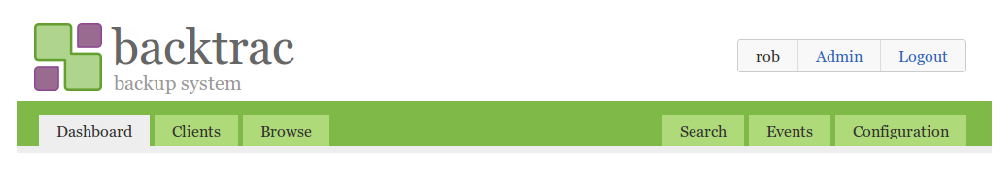
\includegraphics[width=\textwidth]{backtrac-header}
    \end{center}
    \caption{A screenshot of the header, which is shown atop every page}
    \label{fig:backtrac-header}
\end{figure}

The main navigation system is tab-based, with the current tab highlighted to
clearly show where the user is at any one point in time.

\subsubsection{Dashboard}
\label{sec:implementation-web-dashboard}

The dashboard provides a high-level system overview, giving the administrator
access to the most important information in one place. Figure
\ref{fig:backtrac-dashboard} shows a screenshot of the dashboard page.

The dashboard summarizes the following information:

\begin{itemize}
    \item The utilization of the backup filesystem (i.e. the filesystem which
        the archive is stored on)
    \item The total amount of data protected by the backup system
    \item A graph showing the total amount of protected data over time
    \item The status of the backup server itself (i.e. whether it is running)
    \item A list of recent events
\end{itemize}

Much of the information is shown in a visual format (i.e. a bar showing the
disk utilization and a graph showing historical data) so that it can be
interpreted as quickly as possible by the user. This is important to to ensure
that the web interface performs its purpose well---to provide quick and easy
access to \emph{data}.

\begin{figure}
    \begin{center}
        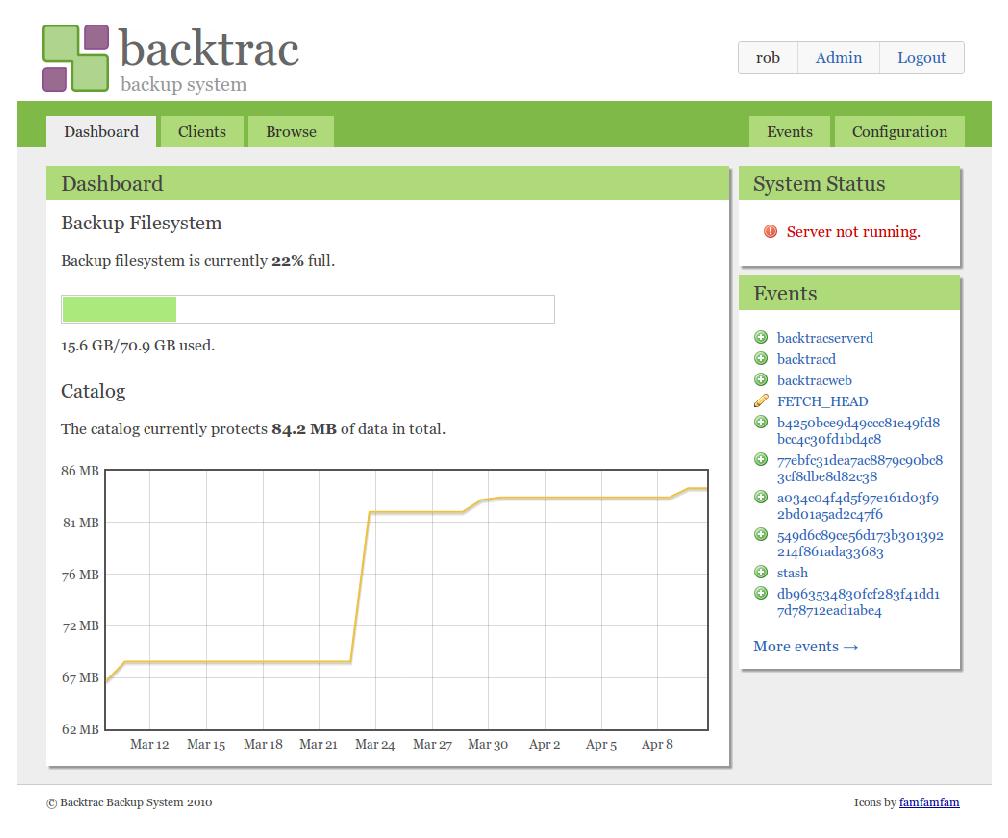
\includegraphics[width=\textwidth]{backtrac-dashboard}
    \end{center}
    \caption{A screenshot of the dashboard page}
    \label{fig:backtrac-dashboard}
\end{figure}

\subsubsection{Clients}
\label{sec:implementation-web-clients}

The clients interface allows the administrator to add, edit or delete backup
clients. When a client is added, it is configured with a secret key and a list
of paths to backup. Figure \ref{fig:backtrac-clients-add} shows a screenshot of
the form used when adding a client.

\begin{figure}[h]
    \begin{center}
        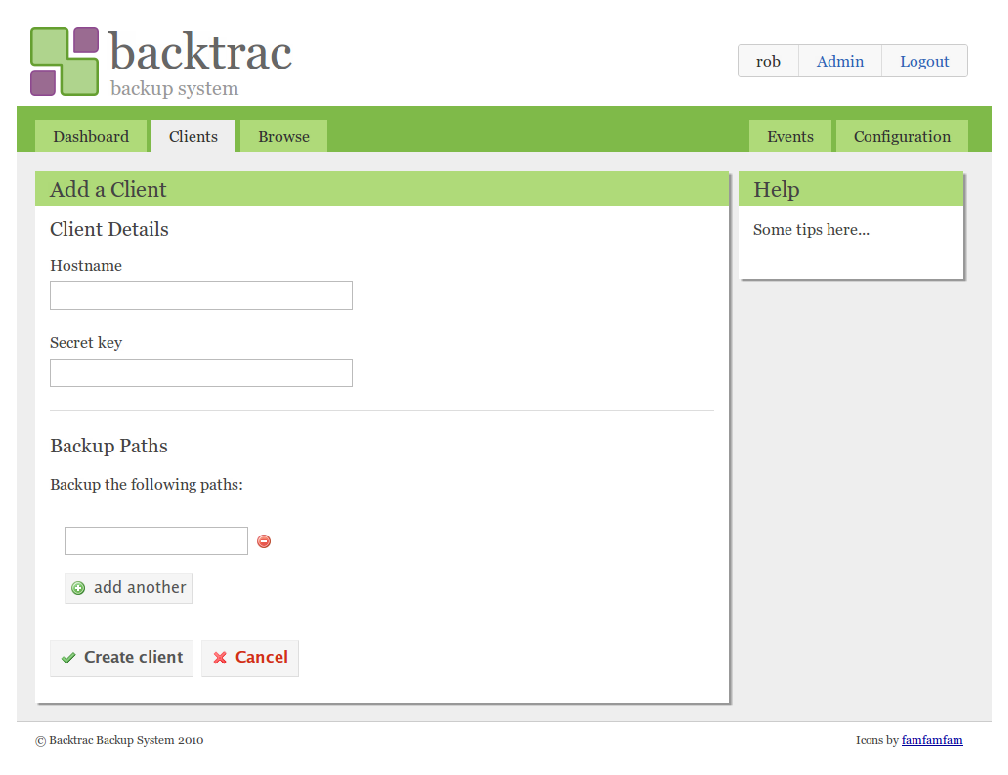
\includegraphics[width=\textwidth]{backtrac-clients-add}
    \end{center}
    \caption{A screenshot of the add client form}
    \label{fig:backtrac-clients-add}
\end{figure}

Note that backup paths can be added quickly and easily, as can exclusions.
These fields can be added or removed dynamically by clicking on the ``add
another'' button, or the remove button next to the relevant field. All
icon-only elements contain alternative text so that they can still be read if
the images are unavailable, or if a screen reader is in use (for the visually
impaired, for example).

\subsubsection{Browse}
\label{sec:implementation-web-browse}

The administrator can browse the catalog of protected items through the web
interface, using the ``browse'' tab. The ``drill-down'' method is used to
provide a familiar way of traversing the filesystem once a client has been
chosen.

When browsing the catalog, the administrator can choose to show or hide deleted
files. This preference is retained throughout the session whilst browsing the
catalog for the same client---to save clicking the same button over and over.
A screenshot of the browsing interface is shown in figure
\ref{fig:backtrac-browse}.

\begin{figure}[h]
    \begin{center}
        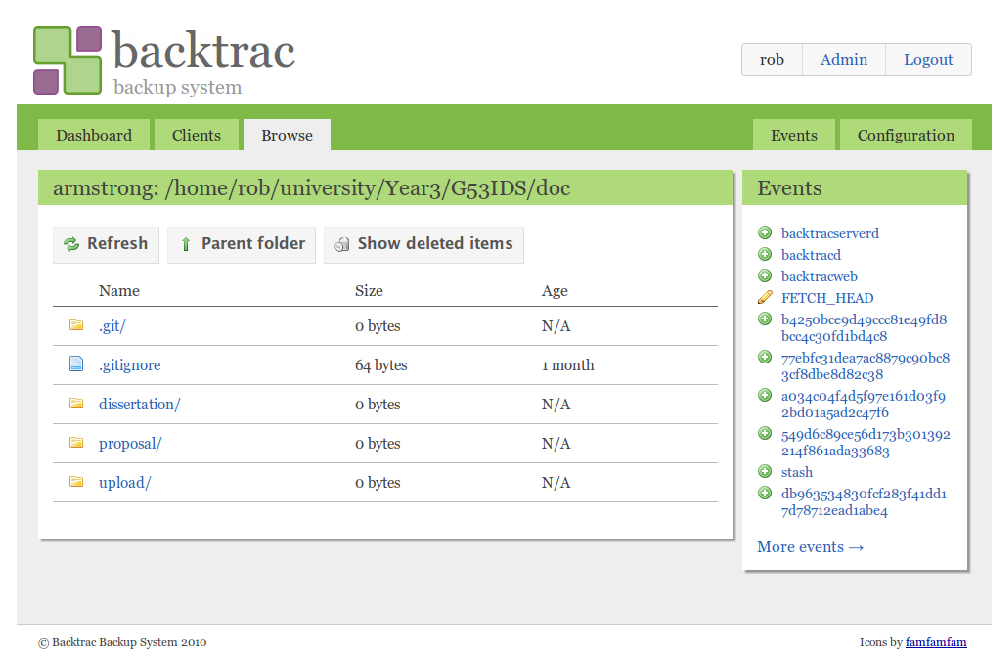
\includegraphics[width=\textwidth]{backtrac-browse}
    \end{center}
    \caption{A screenshot of the catalog browsing interface}
    \label{fig:backtrac-browse}
\end{figure}

Once a file has been selected, a detailed screen shows the different versions
of that file and their respective modification times and sizes. The
administrator can then choose to view one of the versions in the browser (in
the case of a plain text file, image or PDF document), download it, or restore
it to a chosen client. The selected version can be restored to the client from
which it originated, or any other client in the system. Also, it can either be
restored to its original location or another chosen path.

A screenshot of the detailed file view is shown in figure
\ref{fig:backtrac-file-detail}. As shown in the figure, a graph showing the
size of the file over time is also included on the file detail page---showing
how the file has evolved since it was first created.

\begin{figure}[h]
    \begin{center}
        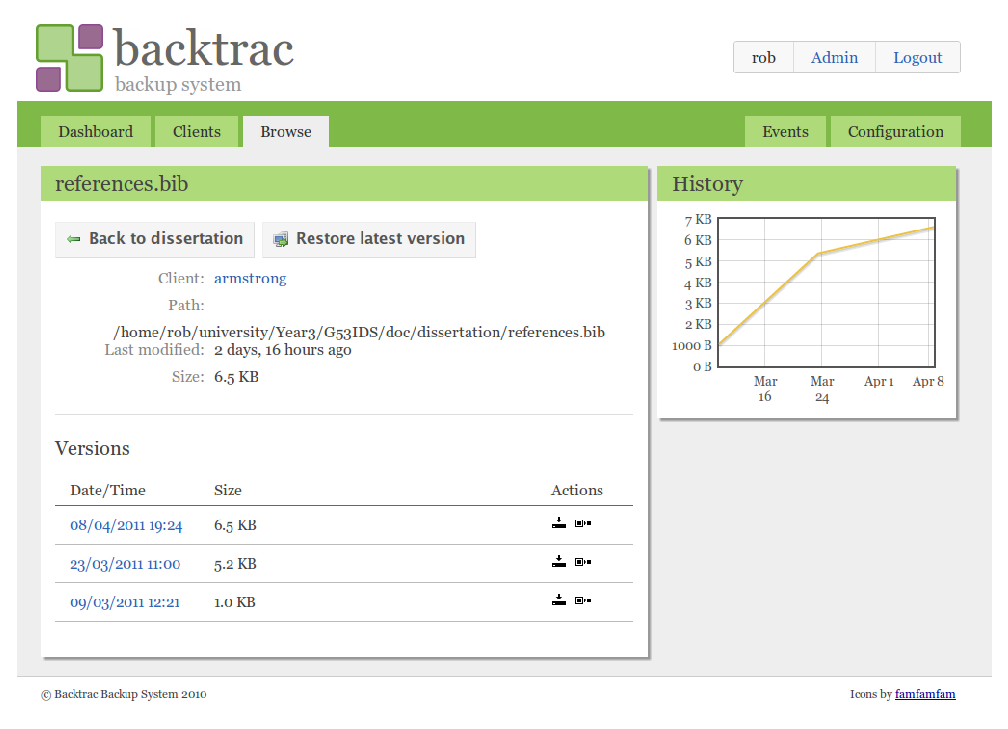
\includegraphics[width=\textwidth]{backtrac-file-detail}
    \end{center}
    \caption{A screenshot of the detailed file view}
    \label{fig:backtrac-file-detail}
\end{figure}

\section{Methodology}

The design described in this section is the result of multiple prototypes,
which eventually evolved into the final system. In the early stages of the
project, initial prototypes were also used to produce a coherent specification
containing the detail required to implement and test the final iteration of the
software itself. These prototypes were used to gather feedback from the
project's industrial sponsor, \emph{Servat, Ltd.}, and to refine the technical
design.

Initially, a fully web-based design was chosen, due to the author's experience
with web technologies. Based on this design, a prototype was developed which
provided a rich RESTful API via the web interface, through which the backup
clients would interact with the server. This essentially removes the need for
a backup server, simplifying the architecture somewhat.

This simplified architecture, however, quickly proved to be unsuitable for the
purpose in hand, due to the overhead incurred when using HTTP, and was revised.
The next prototype used the Twisted framework for communication, which proved
to be extremely powerful and much more suited to the job. The architecture of
this prototype eventually evolved into the final design described by this
document.

A detailed discussion of the methodology used in this project is included in
section \ref{sec:implementation-methodology}.
